\documentclass[book]{magnolia}

\magtex{tex_driver={pdftex},
        tex_packages={float,caption,titling,epigraph,minitoc,slashbox,tabularx,cancel,pgfplots,xypic,nicefrac},
        tex_pstricks={pstricks,pst-plot}}
\magfiche{document_nom={Cours de Sup},
          auteur_nom={François Fayard},
          auteur_mail={fayard.prof@gmail.com}}
\magcours{cours_matiere={maths},
          cours_niveau={mpsi},
          cours_chapitre_numero={11},
          cours_chapitre={Dérivation}}
% \magmisenpage{misenpage_presentation={tikzvelvia},
%           misenpage_format={presentation},
%           misenpage_nbcolonnes={1},
%           misenpage_preuve={non},
%           misenpage_sol={non}}
\magmisenpage{}
\maglieudiff{}
\magprocess

\usepackage[scale=3]{ccicons}
\title{{\Huge\bf Cours de Mathématiques}\\\vspace{1cm}
%       \textbf{\Huge 2022--2023}\\
       \textbf{\Huge Maths Sup -- Tome II}\\\vspace{1cm}
      %  \textsc{L. Bouyge-Bono, F. Fayard, V. Lambert}\\\vspace{1cm}
       \textsc{F. Fayard}\\\vspace{1cm}
       
\includegraphics[width=8cm]{../../Commun/Images/lazos-bde-2024.png}\\%\vspace{1cm}
       
\includegraphics[width=8cm]{../../Commun/Images/lazos.png}}
% \author{{\sc François Fayard}, {\sc Victor Lambert}}
% \date{3 Août 2020 -- 1a20aa}

% \pretitle{%
%   \begin{center}
%   
\includegraphics[width=12cm]{/Users/fayard/Desktop/lazos.png}\\[\bigskipamount]
% }
% \posttitle{\end{center}}

\mtcsettitle{minitoc}{}
\mtcsettitle{secttoc}{Table des matières}
\mtcsettitle{parttoc}{Table des matières}

\usetikzlibrary{positioning}
% \lstset{%
%   frame            = tb,    % draw frame at top and bottom of code block
%   tabsize          = 1,     % tab space width
%   numbers          = none,  % display line numbers on the left
%   framesep         = 3pt,   % expand outward
%   framerule        = 0.4pt, % expand outward 
%   commentstyle     = \color{green},      % comment color
%   keywordstyle     = \color{blue},       % keyword color
%   stringstyle      = \color{blue},    % string color
%   backgroundcolor  = \color{colorLazoBlue1Light}, % backgroundcolor color
%   showstringspaces = false,              % do not mark spaces in strings
%   basicstyle       = \ttfamily,
%   breaklines       = true
% }

\input{vc.tex}

\begin{document}

\maketitle

La version de ce document est la \textsc{\GITAbrHash}.\\

Merci à tous les élèves des lycées Janson de Sailly, du Parc et des Lazaristes pour leurs remarques et corrections. Je remercie
particulièrement \nom{Samuel Auroy}, \nom{Antonin Barbier}, \nom{Amin Belfkira}, \nom{Martin Bot}, \nom{Alexandre Brousse}, \nom{Élodie Brun}, \nom{Damien Callendrier}, \nom{Lauren Calvosa}, \nom{Sylvain Crosnier}, \nom{Enguerrand De Jaegere}, \nom{Thibaud De Valicourt}, \nom{Victor Déru}, \nom{Raphaël Des Boscs}, \nom{Grégoire Dhimoïla}, \nom{Léo Duhamel-Callot}, \nom{Sacha Evrard}, \nom{Axel Faou}, \nom{Titouan Francheteau}, \nom{Hélène Ghaleb}, \nom{Cédric Holocher},
\nom{Maxime Joubert}, \nom{Maxime Lombard}, \nom{Mira Maamri}, \nom{Gauthier Malandrin}, \nom{Pierre-Antoine Nguyen},
\nom{Hilaire Oudinot}, \nom{Eliott Pradeleix}, \nom{Yann-Ellie Ravon}, \nom{Sixtine Reynaud}, \nom{Vivien Thienot},
\nom{Carole Vacherand}, \nom{Camille Vialet}, \nom{Paul Vilars} et \nom{Antonin Villepontoux}.\\

Je tiens enfin à remercier mes anciens professeurs et
collègues qui ont eu une influence sur la rédaction de ce document~: \nom{Walter Appel}, \nom{Bruno Arsac}, \nom{Jean-Pierre Barani}, \nom{Vincent Bayle}, \nom{Christophe Bertault}, \nom{Laurence Bouyge}, \nom{Gilles Chaffard}, \nom{Alain Chillès}, \nom{Denis Choimet}, \nom{Vincent Clapiès}, \nom{Gérard Esposito}, \nom{Stéphane Gonnord}, \nom{Victor Lambert}, %
%\nom{Pierre-Louis Lions},
\nom{Frédéric Morlot}, \nom{Franz Ridde}, \nom{Emmanuel Roblet} et \nom{Alain Troesch}.\\
%, \nom{Cédric Villani}.\\
\vfill


\begin{center}
  \ccbysa\\
  \vspace{2ex}
  This work is licensed under a Creative Commons\\
  Attribution-ShareAlike 4.0 International License.\\
  \url{https://creativecommons.org/licenses/by-sa/4.0/legalcode.fr}\\
  \vspace{2ex}
  La dernière version de ce document ainsi que\\
  les sources \LaTeX{} sont disponibles à l'adresse\\
  \url{https://github.com/FayardProf/Maths-MPSI-MP2I}
  \end{center}
  \vspace{2ex}
  \begin{center}
  \textbf{Vous êtes autorisés à~:}
  \end{center}
  \vspace{2ex}
  \begin{itemize}
  \item \textbf{Partager}~: copier, distribuer et communiquer le matériel par tous les moyens et sous tous formats.
  \item \textbf{Adapter}~: remixer, transformer et créer à partir du matériel
  pour toute utilisation, y compris commerciale.
  \end{itemize}
  \vspace{2ex}
  \begin{center}
  \textbf{Selon les conditions suivantes~:}
  \end{center}
  \vspace{2ex}
  \begin{itemize}
    \item \textbf{Attribution}~: Vous devez créditer l'œuvre, intégrer un lien vers la licence et indiquer si des modifications ont été effectuées à l'œuvre. Vous devez indiquer ces informations par tous les moyens raisonnables, sans toutefois suggérer que l'offrant vous soutient ou soutient la façon dont vous avez utilisé son œuvre.
    \item \textbf{Partage dans les mêmes conditions}~: Dans le cas où vous effectuez un remix, que vous transformez, ou créez à partir du matériel composant l'œuvre originale, vous devez diffuser l'œuvre modifiée dans les même conditions, c'est à dire avec la même licence avec laquelle l'œuvre originale a été diffusée.
    \item \textbf{Pas de restrictions complémentaires}~: Vous n'êtes pas autorisé à appliquer des conditions légales ou des mesures techniques qui restreindraient légalement autrui à utiliser l'œuvre dans les conditions décrites par la licence.
    \end{itemize}

\setcounter{chapter}{4}

\tableofcontents

% \part{Sup}



\chapter{Fonctions usuelles}
\setcounter{numeroexercicecours}{1}
\documentclass{magnolia}

\magtex{tex_driver={pdftex},
        tex_packages={epigraph,xypic}}
\magfiche{document_nom={Fonctions usuelles},
          auteur_nom={François Fayard},
          auteur_mail={fayard.prof@gmail.com}}
\magcours{cours_matiere={maths},
          cours_niveau={mpsi},
          cours_chapitre_numero={3},
          cours_chapitre={Fonctions usuelles}}
\magmisenpage{misenpage_presentation={tikzvelvia},
          misenpage_format={a4},
          misenpage_nbcolonnes={1},
          misenpage_preuve={non},
          misenpage_sol={non}}
\maglieudiff{}
\magprocess

\begin{document}

%BEGIN_BOOK
\setlength\epigraphwidth{.6\textwidth}
\epigraph{\og En mathématiques, on ne comprend pas les choses, on s’y habitue.\fg}{--- \textsc{John Von Neumann (1903--1957)}}
\setlength\epigraphwidth{.5\textwidth}
\epigraph{\og Le logarithme de \nom{John Napier}, en réduisant leur travail, a doublé la vie des astronomes.\fg}{--- \textsc{Pierre-Simon Laplace (1749--1827)}}
\setlength\epigraphwidth{.3\textwidth}
\epigraph{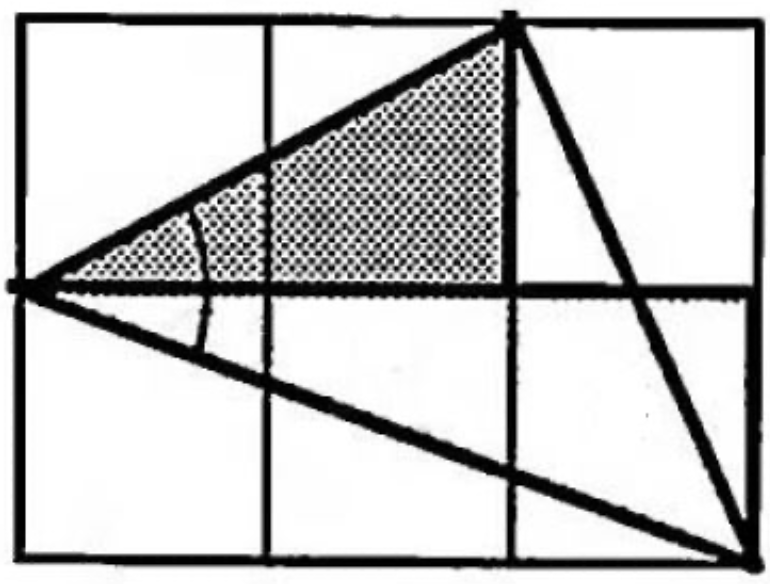
\includegraphics[width=0.9\textwidth]{../../Commun/Images/maths-cours-machin.png}\\
\og $\arctan\frac{1}{2}+\arctan\frac{1}{3}=\frac{\pi}{4}.$ \fg}{--- \textsc{Leonhard Euler (1707--1783)}}

\magtoc

\section{Logarithme, exponentielle, puissance}
\subsection{Logarithme népérien}
\begin{definition}[utile=-3]
On appelle \emph{logarithme népérien} et on note $\ln$ l'unique primitive sur $\RPs$ de la fonction $x\mapsto 1/x$ qui s'annule en~1.
\[\dspappli{\ln}{\RPs}{\R}{x}{\integinv{1}{x}{t}{t}}\]
\end{definition}

\begin{remarqueUnique}
\remarque Le nom $\ln$ est à la fois l'acronyme de logarithme naturel et de
  logarithme népérien (en hommage à \nom{John Napier}, mathématicien Écossais,
  1550--1617).
\end{remarqueUnique}

\begin{proposition}[utile=-3]
\begin{itemize}
\item $\ln$ est continue sur $\RPs$.
\item $\ln$ est dérivable sur $\RPs$ et
  \[\forall x\in\RPs \qsep \ln' x=\frac{1}{x}.\]
% \item $\ln$ est $\classec{\infty}$ sur $\RPs$.
\end{itemize}
\end{proposition}

\begin{preuve}
Tout vient de la définition précédente.
\end{preuve}

\begin{remarqueUnique}
\remarque La fonction
  \[\dspappli{f}{\Rs}{\R}{x}{\ln\abs{x}}\]
  est dérivable sur $\Rs$ et, pour tout $x\in\Rs$, $f'(x)=1/x$. Autrement dit, sur $\Rs$
  \[\priminv{x}{x}=\ln\abs{x}.\]
\end{remarqueUnique}

\begin{proposition}[utile=-3]
\begin{eqnarray*}
                   & & \ln 1=0,\\
\forall x,y\in\RPs, & & \ln\p{xy}=\ln x+\ln y,\\
\forall x\in\RPs, & & \ln\p{1/x}=-\ln x,\\
\forall x\in\RPs \qsep \forall n\in\Z, & & \ln x^n=n\ln x.
\end{eqnarray*}
\end{proposition}

\begin{preuve}
On définit $\dspappli{\varphi}{\RPs}{\R}{y}{\ln(xy)-\ln(x)-\ln(y)}$ et on montre que $\varphi$ est nulle en la dérivant.
La suite en découle.
\end{preuve}

\begin{proposition}[utile=-3]
\[\forall x\in\RPs \qsep \forall n\in\Ns \qsep
  \ln\sqrt[n]{x}=\frac{1}{n}\cdot\ln x.\]
\end{proposition}

\begin{proposition}[utile=-3]
$\ln$ est strictement croissante sur $\RPs$. De plus
\[\ln x \tendvers{x}{+\infty} +\infty \et
  \ln x \tendvers{x}{0} -\infty.\]
\end{proposition}

\begin{preuve}
$\ln$ admet une limite dans $\overline{\R}$. Il suffit alors de montrer qu'elle n'est pas majorée, ce qu'on peut faire, via $\ln(2^n)=n\ln(2)$.

$\ln(x)=-\ln(1/x)$ pour l'autre.
\end{preuve}
\begin{exoUnique}
\exemple Résoudre l'inéquation $\ln\abs{x+1}-\ln\abs{2x+1}\leq\ln 2$.
  \begin{sol}
On réunit tous les $\ln$ du même côté puis on enlève les log puis on élève au carré (par équivalence) et on obtient $x\in\interof{-\infty}{-3/5}\cup\interfo{-1/3}{+\infty}$. 
  \end{sol}
\end{exoUnique}

\begin{proposition}[utile=-3]
$\ln$ réalise une bijection de $\RPs$ dans $\R$.
\end{proposition}

\begin{preuve}
limites + stricte croissance.
\end{preuve}

\begin{definition}[utile=-3]
Il existe un unique réel, noté $\e$ et appelé \emph{nombre de \nom{Néper}}, tel que $\ln \e=1$.
\end{definition}



\begin{preuve}
$n\ln\sqrt[n]{x}=\ln\p{\p{\sqrt[n]{x}}^{n}}=\ln(x)$.
\end{preuve}


\begin{proposition}[utile=-3]
\[\forall x\in\intero{-1}{+\infty} \qsep \ln\p{1+x}\leq x.\]  
\end{proposition}

\begin{preuve}
Simple étude de fonction.
\end{preuve}


\begin{exoUnique}
\exemple Montrer que pour tout $n\in\Ns$,
  $\frac{1}{n+1}\leq\ln\p{1+\frac{1}{n}}\leq\frac{1}{n}$.
\end{exoUnique}

\begin{sol}
\nom{Victor}~: $\ln\p{1+\frac{1}{n}}=\ln(n+1)-\ln(n)$ qu'on voit comme une intégrale qu'on encadre.\\
\nom{François}~: Soit $n\in\Ns$. Alors
\[\ln\p{1+\frac{1}{n}}\leq\frac{1}{n}\]
d'après la proposition précédente. Pour la première inégalité, on a
\[\ln\p{1+\frac{1}{n}}=\ln\p{\frac{n+1}{n}}=-\ln\p{\frac{n}{n+1}}=-\ln\p{1-\frac{1}{n+1}}.\]
Or, en utilisant la proposition précédente
\[\ln\p{1-\frac{1}{n+1}}\leq -\frac{1}{n+1}\]
donc
\[\ln\p{1+\frac{1}{n}}\geq\frac{1}{n+1}.\]
\end{sol}

\begin{proposition}[utile=-3]
\[\frac{x}{\ln x}\tendvers{x}{+\infty} +\infty, \qquad
  x\ln x\tendvers{x}{0} 0,\]
\[\frac{\ln\p{1+x}}{x} \tendvers{x}{0} 1.\]  
\end{proposition}

\begin{preuve}
$\ln(u)\leq u$ appliqué en $\sqrt{x}$ donne $\frac{\ln x}{x}\tendvers{x}{+\infty} 0$ par valeur supérieure.

$x\ln(x)=-\dfrac{\ln(1/x)}{1/x}$ permet de conclure pour la deuxième limite.

Taux d'accroissement pour la dernière.

\end{preuve}

\begin{center}
\begin{pdfpic}
\readdata{\listePln}{graph/graphe_ln.txt}
\psset{xunit=2.3cm,yunit=2.3cm}
\begin{pspicture}(-1,-2.2)(4.2,1.6)
  \psaxes[labels=none]{->}(0,0)(-1,-2.2)(4.2,1.6)
  \dataplot[plotstyle=curve,linewidth=2pt]{\listePln}
  \psline[linewidth=0.5pt](-0.8,-1.8)(2.38,1.38)
  \uput[ul](2,1){$y=x-1$}
  \uput[d](1,0){1}
  \uput[d](2.718,0){${\rm e}$}
  \psline[linestyle=dashed,linewidth=0.5pt](2.718,0)(2.718,1)
  \psline[linestyle=dashed,linewidth=0.5pt](2.718,1)(0,1)
  \uput[l](0,1){1}
  \uput[r](4.2,0){$x$}
  \uput[r](0,1.6){$y$}
  \uput[dr](3.2,1.163){$y=\ln x$}
\end{pspicture}
\end{pdfpic}
\end{center}


\subsection{Exponentielle}

\begin{definition}[utile=-3]
Pour tout $y\in\R$, il existe un unique $x\in\RPs$ tel que $\ln x=y$; on le
note $\exp y$. On définit ainsi la fonction
\[\dspappli{\exp}{\R}{\RPs}{y}{\exp y.}\]
\end{definition}

\begin{remarques}
\remarque Autrement dit, $\exp$ est la bijection réciproque de $\ln$.
\remarque Par définition
  \[\forall x\in\R\qsep \exp x>0.\]
\end{remarques}

\begin{proposition}[utile=-3]
\begin{eqnarray*}
\forall x\in\R, & & \ln\p{\exp x}=x,\\
\forall x\in\RPs, & & \exp\p{\ln x}=x.    
\end{eqnarray*}
\end{proposition}

\begin{proposition}[utile=-3]
$\exp$ réalise une bijection de $\R$ dans $\RPs$.
\end{proposition}

\begin{proposition}[utile=-3]
\begin{eqnarray*}
\exp 0=1, & & \exp 1=\e,\\
\forall x,y\in\R, & & \exp\p{x+y}=\exp(x)\exp(y),\\
\forall x\in\R, & & \exp\p{-x}=\frac{1}{\exp x},\\
\forall x\in\R \qsep \forall n\in\Z, & & \exp\p{nx}=\p{\exp x}^n.
\end{eqnarray*}
\end{proposition}

\begin{preuve}
$\exp(x+y)=\exp(\ln(\exp(x))+\ln(\exp(y)))$...
\end{preuve}

\begin{proposition}[utile=-3]
$\exp$ est strictement croissante sur $\R$. De plus
\[\exp x\tendvers{x}{-\infty} 0 \et \exp x\tendvers{x}{+\infty} +\infty.\]
\end{proposition}

\begin{preuve}
Croissante par bijection réciproque d'une fonction croissante et les limites car elle est bijective.
\end{preuve}


\begin{proposition}[utile=-3]
\begin{itemize}
\item $\exp$ est continue sur $\R$.
\item $\exp$ est dérivable sur $\R$ et
  \[\forall x\in\R \qsep \exp' x=\exp x.\]
% \item $\exp$ est $\classec{\infty}$ sur $\R$.
\end{itemize}
\end{proposition}

\begin{preuve}
$f$ bijective et dérivable telle que $f'$ ne s'annule pas sur $I$, alors $f^{-1}$ est dérivable sur $I$ et $(f^{-1})'=1/(f'\circ f^{-1})$.
\end{preuve}

\begin{proposition}[utile=-3]
\[\forall x\in\R \qsep \exp x \geq 1+x.\]
\end{proposition}
\begin{preuve}
Si $x\leq -1, 1+x\leq 0 \leq \exp x$. Sinon, $\ln(1+x)\leq  x$ puis passage à l'exponentielle.
\end{preuve}

\begin{exos}
\exemple Montrer que
  \[\forall x<1 \qsep \exp x\leq\frac{1}{1-x}.\]
  \begin{sol}
  $\forall x\in\R \qsep \exp (-x) \geq 1-x.$ Si $x<1$, $1-x>0$ et par décroissance de la fonction inverse sur $\RPs$, on a le résultat.
  \end{sol}
\exemple Soit $a,b\in\R$ tels que $0<a<b$. Montrer que
  \[\forall x\in\RPs \qsep 0<b\exp(-ax)-a\exp(-bx)<b-a.\]
  \begin{sol}
  On dérive la fonction à l'intérieur. Elle est décroissante, vaut $b-a$ en $0$ et sa limite en l'infini est $0$.
  \end{sol}
\end{exos}

\begin{proposition}[utile=-3]
\[\frac{\exp x}{x} \tendvers{x}{+\infty} +\infty, \qquad
  x\exp x \tendvers{x}{-\infty} 0,\]
\[\frac{\exp(x)-1}{x} \tendvers{x}{0} 1.\]
\end{proposition}

\begin{preuve}
 On peut poser $x=\ln u$ et se ramener à la limite de $u/\ln(u)$ en $+\infty$.

$x\exp(x)=-x/\exp(-x)$ permet d'avoir la deuxième limite.

Taux d'accroissement pour la troisième.
\end{preuve}

\begin{center}
\begin{pdfpic}
\readdata{\listePln}{graph/graphe_ln.txt}
\readdata{\listePexp}{graph/graphe_exp.txt}
\psset{xunit=1.8cm,yunit=1.8cm}
\begin{pspicture}(-2.2,-2.2)(4.2,4.2)
  \psaxes[labels=none]{->}(0,0)(-2.2,-2.2)(4.2,4.2)
  \dataplot[plotstyle=curve,linestyle=dashed,linewidth=0.5pt]{\listePln}
  \dataplot[plotstyle=curve,linewidth=2pt]{\listePexp}
  \uput[d](1,0){1}
  \uput[l](0,2.718){${\rm e}$}
  \psline[linestyle=dashed,linewidth=0.5pt](0,2.718)(1,2.718)
  \psline[linestyle=dashed,linewidth=0.5pt](1,2.718)(1,0)
  \psline[linewidth=0.5pt](-2,-2)(4,4)
  \psline[linewidth=0.5pt](-2,-1)(3,4)
  \uput[l](0,1){1}
  \uput[r](4.2,0){$x$}
  \uput[r](0,4.2){$y$}
  \uput[dr](3.2,1.163){$y=\ln x$}
  \uput[r](1.2527,3.5){$y=\exp x$}
  \uput[r](1,2){$y=x+1$}
  \uput[dr](3,3){$y=x$}
\end{pspicture}
\end{pdfpic}
\end{center}

\subsection{Logarithme et exponentielle en base $a$}

\begin{definition}[utile=-3]
Soit $a\in\RPs\setminus\ens{1}$. On appelle \emph{logarithme en base $a$} et on note
$\log_a$ la fonction
\[\dspappli{\log_a}{\RPs}{\R}{x}{\frac{\ln x}{\ln a}.}\]
\end{definition}

\begin{remarqueUnique}
\remarque Le logarithme népérien est le logarithme en base
  $\e$. Si $a=10$, on obtient le logarithme décimal qui est utilisé  en
  physique (pour définir les décibels) et en chimie (pour définir le pH).% Enfin, si $a=2$, on obtient le
%  logarithme binaire, utilisé en informatique.
%\remarque En \verb+Maple+, les fonctions \verb+ln+ et \verb+log+ font toutes
%  les deux référence au logarithme népérien. Pour obtenir le logarithme de $x$
%  en base $a$, on utilisera la commande \verb+log[a](x)+. Enfin, la fonction
%  \verb+log10+ fait référence au logarithme en base 10.
\end{remarqueUnique}

\begin{exoUnique}
\exo Résoudre le système
  \[\begin{cases}
    2\log_x y+2\log_y x=-5 &\\
    xy=\e. &
    \end{cases}\]
  \begin{sol}
  On remplace $x$ ou $y$ grâce à la deuxième équation puis on pose $u=\ln(y)/(1-\ln(y))$. On obtient $u=-2$ ou $u=-1/2$ donc on trouve $x=e^2$ et $y=1/e$ et inversement.    
  \end{sol}
\end{exoUnique}

\begin{proposition}[utile=-3]
Soit $a\in\RPs\setminus\ens{1}$. Alors
\begin{eqnarray*}
\forall x,y\in\RPs, & & \log_a \p{xy}=\log_a  x+\log_a  y,\\
\forall x\in\RPs, & & \log_a \p{1/x}=-\log_a  x,\\
\forall x\in\RPs \qsep \forall n\in\Z, & & \log_a  x^n=n\log_a x.
\end{eqnarray*}
\end{proposition}

\begin{definition}[utile=-3]
Soit $a\in\RPs\setminus\ens{1}$. Alors, pour tout $y\in\R$, il existe un unique
$x\in\RPs$ tel que $\log_a x=y$; on le note $\exp_a y$ et on a
\[\exp_a y=\exp\p{y\ln a}.\]
On définit ainsi la fonction
\[\dspappli{\exp_a}{\R}{\RPs}{y}{\exp\p{y \ln a .}}\]
\end{definition}

\begin{remarqueUnique}
\remarque Lorsque $a=\e$, on retrouve la fonction exponentielle.  
\end{remarqueUnique}

% \begin{proposition}[utile=-3]
% Soit $a\in\RPs\setminus\ens{1}$. Alors
% \begin{eqnarray*}
% \exp_a  0=1 & & \exp_a  1=a\\
% \forall x,y\in\R & & \exp_a \p{x+y}=\exp_a (x)\exp_a (y)\\
% \forall x\in\R & & \exp_a \p{-x}=\frac{1}{\exp_a  x}\\
% \forall x\in\R \qsep \forall n\in\Z & & \exp_a \p{nx}=\p{\exp_a  x}^n
% \end{eqnarray*}
% \end{proposition}

\subsection{Fonction puissance}

\begin{definition}[utile=-3]
Pour $x\in\RPs$ et $y\in\R$, on définit $x^y$ par
\[x^y\defeq\exp\p{y \ln x}.\]
\end{definition}

\begin{remarques}
\remarque En particulier, pour tout $x\in\R$, $\exp x=\e^x$. Plus généralement,
   si $a\in\RPs\setminus\ens{1}$
   \[\forall x\in\R \qsep \exp_a(x)=a^x.\]
   On utilisera désormais cette notation pour désigner l'exponentielle ainsi que
   l'exponentielle en base $a$.
\remarque Afin de dériver une fonction de la forme $f(x)\defeq u(x)^{v(x)}$, il est recommandé de la mettre sous la forme
  \[f(x)=\e^{v(x)\ln\p{u(x)}}.\]
\end{remarques}

\begin{exos}
\exemple Résoudre l'équation $x^{\sqrt{x}}=\sqrt{x}^{\ x}$.
  \begin{sol}
  Les solutions de cette équation sont 1 et 4.
  \end{sol}
\exemple Calculer $\fracd{}{x}\p{x^x}$.
  \begin{sol}
  On trouve $\p{\ln x+1}x^x$.
  \end{sol}
\end{exos}

\begin{definition}[utile=-3]
Soit $a\in\R$. On appelle fonction puissance, la fonction définie sur $\RPs$
\[\dspappli{\phi_a}{\RPs}{\R}{x}{x^a .}\]
\end{definition}

\begin{proposition}[utile=-3]
\begin{eqnarray*}
\forall x\in\RPs \qsep x^0=1, & & \forall a\in\R \qsep 1^a=1,\\
\forall x\in\RPs \qsep \forall a,b\in\R, & & x^{a+b}=x^a x^b,\\
\forall x\in\RPs \qsep \forall a\in\R, & & x^{-a}=1/x^a,\\
\forall x,y\in\RPs \qsep \forall a\in\R, & & \p{xy}^a=x^a y^a,\\
\forall x\in\RPs \qsep \forall a,b\in\R, & & \p{x^a}^b=x^{ab},\\
\forall x\in\RPs \qsep \forall a\in\R, & & \ln\p{x^a}=a\ln x .
\end{eqnarray*}
\end{proposition}

\begin{proposition}[utile=-3]
Soit $a\in\R$. La fonction $\phi_a:x\mapsto x^a$ définie sur $\RPs$ est
\begin{itemize}
\item continue sur $\RPs$.
\item dérivable sur $\RPs$ et
  \[\forall x\in\RPs \qsep \phi_a'(x)=a x^{a-1}.\]
% \item $\classec{\infty}$ sur $\RPs$.
\end{itemize}
\end{proposition}

% \begin{remarques}
% \remarque Soit $f_1,\ldots,f_n$ des fonctions dérivables à valeurs
%   strictement positives sur $\mathcal{D}$ et $\alpha_1,\ldots,\alpha_n\in\R$.
%   On définit la fonction $f$ sur $\mathcal{D}$ par
%   \[\forall x\in\mathcal{D} \qsep f(x)=f_1(x)^{\alpha_1}\cdots
%     f_n(x)^{\alpha_n}\]
%   Alors $f$ est dérivable sur $\mathcal{D}$ et
%   \[\forall x\in\mathcal{D} \qsep \frac{f'(x)}{f(x)}=
%     \alpha_1\cdot\frac{f_1'(x)}{f_1(x)}+\cdots+\alpha_n\cdot
%     \frac{f_n'(x)}{f_n(x)}\]
%   Cette relation reste vraie si l'on suppose juste que les fonctions $f_k$
%   sont dérivables et ne s'annulent pas, dans le cas bien sur où l'expression
%   $f_1(x)^{\alpha_1}\cdots f_n(x)^{\alpha_n}$ conserve un sens (c'est-à-dire
%   lorsque les $\alpha_k$ associés aux fonctions $f_k$ prenant des valeurs
%   strictement négatives sont entiers). On a donc
%   \[\forall x\in\mathcal{D} \qsep f'(x)=\sum_{k=1}^n \alpha_k \cdot
%     f_1(x)^{\alpha_1}\cdots f_k'(x)f_k^{\alpha_k-1}(x)\cdots f_n(x)^{\alpha_n}\]
%   Cette relation reste d'ailleurs vraie si l'on suppose juste les fonctions
%   $f_k$ dérivables dans la mesure où l'expression $f_1(x)^{\alpha_1}\cdots
%   f_n(x)^{\alpha_n}$ conserve un sens (c'est-à-dire lorsque les $\alpha_k$
%   associés aux fonctions $f_k$ pouvant s'annuler sont entiers naturels).
% \end{remarques}

% \begin{exos}
% \exemple Calculer
%   \[\fracd{}{x}\p{\frac{e^x}{\sqrt{1+x^2}}}, \qquad \fracd{}{x}\p{
%     \frac{x+2}{\sqrt[3]{1+x^2}}}.\]
% \end{exos}

\begin{proposition}[utile=-3]
Soit $a\in\R$. Alors
\[x^a \tendvers{x}{+\infty}
  \begin{cases}
  +\infty & \text{si $a>0$}\\
  1 & \text{si $a=0$}\\
  0 & \text{si $a<0$}
  \end{cases} \et
  x^a \tendvers{x}{0}
  \begin{cases}
  0 & \text{si $a>0$}\\
  1 & \text{si $a=0$}\\
  +\infty & \text{si $a<0$.}
  \end{cases}\]
\end{proposition}


\begin{remarqueUnique}
\remarque Si $a>0$, on définit $0^a$ en posant $0^a\defeq 0$. La fonction
  \[\dspappli{\phi_a}{\RP}{\R}{x}{x^a}\]
  est continue sur $\RP$ et dérivable sur
  \begin{itemize}
  \item $\RP$ lorsque $a\geq 1$ avec
    \[\forall x\in\RP \qsep \phi_a'(x)=a x^{a-1}.\]
  \item $\RPs$ lorsque $a<1$ avec
    \[\forall x\in\RPs \qsep \phi_a'(x)=a x^{a-1}.\]
  \end{itemize}
\end{remarqueUnique}

\begin{center}
\begin{pdfpic}
\readdata{\listePpuissa}{graph/graphe_puissa.txt}
\readdata{\listePpuissb}{graph/graphe_puissb.txt}
\readdata{\listePpuissc}{graph/graphe_puissc.txt}
\readdata{\listePpuissd}{graph/graphe_puissd.txt}
\readdata{\listePpuisse}{graph/graphe_puisse.txt}
\psset{xunit=4cm,yunit=4cm}
\begin{pspicture}(-0.2,-0.2)(2.2,2.2)
  \psaxes[labels=none]{->}(0,0)(-0.2,-0.2)(2.2,2.2)
  \dataplot[plotstyle=curve,linewidth=2pt]{\listePpuissa}
  % \dataplot[plotstyle=curve,linewidth=2pt]{\listePpuissb}
  \dataplot[plotstyle=curve,linewidth=2pt]{\listePpuissc}
  \dataplot[plotstyle=curve,linewidth=2pt]{\listePpuissd}
  \dataplot[plotstyle=curve,linewidth=2pt]{\listePpuisse}
  \psline[linewidth=2pt](0,1)(2,1)
  \uput[r](2.2,0){$x$}
  \uput[r](0,2.2){$y$}
  \uput[dr](1.8,0.5){$y=x^{-1}=1/x$}
  \uput[dr](1.8,1){$y=x^0=1$}
  \uput[ur](1.8,1.25){$y=x^{\frac{1}{3}}=\sqrt[3]{x}$}
  \uput[dr](1.8,1.8){$y=x$}
  \uput[r](1.26,2){$y=x^3$}
  \uput[d](1,0){1}
  \uput[l](0,1){1}
\end{pspicture}
\end{pdfpic}
\end{center}

\begin{proposition}
  \[\forall n\in\Ns\qsep \forall x\geq 0\qsep \sqrt[n]{x}=x^{\frac{1}{n}}.\]
\end{proposition}

\subsection{Calcul de limite}
\begin{proposition}[utile=-3, nom={Croissances comparées}]
Soit $\alpha,\beta>0$ et $n\in\Ns$. Alors
\[\frac{\e^{\alpha x}}{x^\beta}\tendvers{x}{+\infty} +\infty, \qquad
  \frac{x^\alpha}{\p{\ln x}^\beta}\tendvers{x}{+\infty} +\infty,\]
\[x^\alpha \p{\ln x}^n \tendvers{x}{0} 0.\]
\end{proposition}

\begin{preuve}
$\dfrac{e^{\alpha x}}{x^\beta}=\p{\dfrac{e^{\alpha x/\beta}}{x}}^{\beta}=\p{\dfrac{\alpha}{\beta}}^{\beta}.\p{\dfrac{e^{\alpha x/\beta}}{\alpha x/\beta}}^{\beta}$.

$\dfrac{x^\alpha}{\p{\ln x}^\beta}=\p{\dfrac{x^{\alpha/\beta}}{\ln(x)}}^\beta=\p{\dfrac{\alpha}{\beta}}^\beta\p{\dfrac{x^{\alpha/\beta}}{\ln(x^{\alpha/\beta})}}^\beta$.

$x^\alpha \p{\ln x}^n=\p{x^{\alpha/n}\ln(x)}^n=\p{x^{\alpha/n}\ln(x^{\alpha/n})}^n.\p{\dfrac{n}{\alpha}}^n$.
\end{preuve}

\begin{remarques}
\remarque Mnémotechniquement, on dit qu'en 0 et en $+\infty$, l'exponentielle
  l'emporte sur la puissance qui l'emporte sur le logarithme.
\remarque La technique essentielle dans le calcul des limites est la
  \emph{factorisation par le terme principal}~: lorsqu'on fait face à une somme de termes
  qui tendent vers $\pm\infty$, il est nécessaire de factoriser par le terme qui tend
  \og le plus vite vers l'infini\fg. 
\begin{itemize}
\item Pour calculer la limite en $\pm\infty$ des polynômes, il convient de
  factoriser par le monôme de plus haut degré. Par exemple
  $$2x^3-x^2+1=x^3\p{2-\frac{1}{x}+\frac{1}{x^3}}\tendvers{x}{+\infty}+\infty.$$
\item Pour calculer la limite en $\pm\infty$ des fractions rationnelles, il
  convient de factoriser au numérateur et au dénominateur par le monôme de
  plus haut degré. Par exemple
  
 $$\frac{x^2+2x-3}{2x^2-1}=\frac{1+\frac{2}{x}-\frac{3}{x^2}}
                           {2-\frac{1}{x^2}}\tendvers{x}{+\infty}\frac{1}{2}.$$
\item Pour calculer la limite en $\pm\infty$ des fractions rationnelles en $x$
  et en $\e^x$, il convient d'utiliser les croissances comparées en se
  rappelant que l'exponentielle l'emporte sur les puissances
  en $-\infty$ et en $+\infty$. Par exemple
  \[\e^x-x^5=\e^x\p{1-\frac{x^5}{\e^x}}\tendvers{x}{+\infty} +\infty, \qquad
    \frac{\e^{2x}-2x\e^x}{x^3+3\e^{2x}}=\frac{1-2\frac{x}{\e^x}}
    {3+\frac{x^3}{\e^{2x}}}\tendvers{x}{+\infty}\frac{1}{3}.\]
\item Pour calculer la limite en $+\infty$ ou en $0$ des fractions rationnelles
  en $\ln x,x$ et $\e^x$, il convient d'utiliser les croissances comparées en se
  rappelant que l'exponentielle l'emporte sur les puissances
  qui l'emportent sur le logarithme que ce soit en $+\infty$ ou en $0$.
  % Par exemple
  % $$\frac{\e^x\ln x-x^{1000}+\e^{2x}}{\e^{2x}+\ln x+x}=
  %   \frac{1+\frac{\ln x}{\e^x}-\frac{x^{1000}}{\e^{2x}}}
  %        {1+\frac{\ln x}{\e^{2x}}+\frac{x}{\e^{2x}}}\tendvers{x}{+\infty} 1$$
  % \begin{equation*}
  % \begin{split}
  % \frac{x^3\ln x-x^2\ln^2 x}{x+x\ln x}&=-\frac{x^2\ln^2 x}{x\ln x}\cdot
  %                                \frac{1-\frac{x}{\ln x}}{1+\frac{1}{\ln x}}\\
  %                 &=-\p{x\ln x}\frac{1-\frac{x}{\ln x}}{1+\frac{1}{\ln x}}
  %                   \tendvers{x}{0} 0.
  % \end{split}
  % \end{equation*}
\end{itemize}
\remarque Une autre technique importante est la technique du \emph{changement de variable}. Elle
se base sur le théorème de composition des limites. Le principe en est le suivant.
Étant donné une fonction $f$ définie
au voisinage de $a$, on cherche deux fonctions $g$ et $\bar{u}$ telles que sur
ce voisinage
$$f(x)=g(\bar{u}(x)).$$
Si on connait la limite $l$ de $\bar{u}(x)$ lorsque $x$ tend vers $a$ et la
limite $l'$ de $g(u)$ lorsque $u$ tend vers $l$, alors le théorème de
composition des limites permet de conclure que $f(x)$ tend vers $l'$ lorsque $x$ tend vers $a$.
\end{remarques}








% Une autre technique importante est la technique du \emph{changement de variable}. Elle
% se base sur le théorème de composition des limites. Le principe en est le suivant.
% Étant donné une fonction $f$ définie
% au voisinage de $a$, on cherche deux fonctions $g$ et $\bar{u}$ telles que sur
% ce voisinage
% $$f(x)=g(\bar{u}(x)).$$
% Si on connait la limite $l$ de $\bar{u}(x)$ lorsque $x$ tend vers $a$ et la
% limite $l'$ de $g(u)$ lorsque $u$ tend vers $l$, alors le théorème de
% composition des limites permet de conclure que $f(x)$ tend vers $l'$ lorsque $x$ tend vers $a$.

\begin{exos}
% \item On cherche la limite, si elle existe, de
%   $$\frac{\e^{\e^x}}{x^2}.$$
%   lorsque $x$ tend vers $+\infty$.
%   \begin{sol}
%   On pose $u=\e^x$, donc $x=\ln u$.
%     On a alors~:
%     $$\frac{\e^{\e^x}}{x^2}=\frac{\e^u}{\ln^2 u}.$$
%     Or $u$ tend vers $+\infty$ lorsque $x$ tend vers $+\infty$ et les théorèmes
%     de croissances comparées affirment que $\ln^{-2} u\,\e^u$ tend vers
%     $+\infty$ lorsque $u$ tend vers $+\infty$. On en déduit donc que
%     $$\frac{\e^{\e^x}}{x^2}\tendvers{x}{+\infty}+\infty.$$
%     \end{sol}
% \exo Calculer les limites des expressions suivantes.
%   \[2x^3-x^2+1 \quad\text{en $-\infty$}, \qquad
%     \frac{x^2+2x-3}{2x^2-1} \quad\text{en $-\infty$}.\]
%     \begin{sol}
%     On a
%     \[2x^3-x^2+1=2x^3\left(1-\frac{1}{2x}+\frac{1}{2x^{3}} \right)\tendvers{x}{+\infty}+\infty\]
%     \[\frac{x^2+2x-3}{2x^2-1}=\frac{1+\frac{2}{x}-\frac{3}{x^{2}}}{2\left( 1-\frac{1}{2x^{2}}\right) }\tendvers{x}{+\infty}\frac{1}{2}.\]
%     \end{sol}
\exo Calculer la limite de
  % \[\e^x-x^5 \quad\text{en $+\infty$}, \qquad
  \[\frac{\e^x\ln x-x^{1000}+\e^{2x}}{\e^{2x}+\ln x+x}
    \quad\text{en $+\infty$}.\]
    \begin{sol}
    On a
\[\e^x-x^5=\e^x\left( 1-\frac{x^5}{\e^{x}}\right)\tendvers{x}{+\infty} +\infty\]
\[\frac{\e^x\ln x-x^{1000}+\e^{2x}}{\e^{2x}+\ln x+x} = \frac{\frac{\ln x}{\e^{x}}-\frac{x^{1000}}{\e^{2x}}+1}{1+\frac{\ln x}{\e^{2x}}+\frac{x}{\e^{2x}}}\tendvers{x}{+\infty} 1\]
    \end{sol}
\exo Calculer les limites suivantes
\[\frac{(\ln x)^2}{\e^x} \quad \text{en $+\infty$}, \qquad
  \frac{1}{x}\cdot \e^{-\frac{1}{x^2}} \quad \text{en 0}, \qquad
  \frac{\e^{\e^x}}{x^2} \quad\text{en $+\infty$}, \qquad
  \abs{\ln x}^x \quad \text{en 0 .}\]
  \begin{sol}
    La première tend vers zéro par croissance comparée. Pour la seconde, on a
    \[\frac{\e^{\e^x}}{x^2}=\frac{\e^{\e^x}}{\e^x}\cdot\frac{\e^x}{x^2}\]
    Or, en posant $u=\e^x\tendvers{x}{+\infty}+\infty$, puisque $(\e^u)/u\tendvers{u}{+\infty}$, on en déduit par composition que
    \[\frac{\e^{\e^x}}{\e^x}\tendvers{x}{+\infty}+\infty.\]
    Comme de plus
    \[\frac{\e^x}{x^2}\tendvers{x}{+\infty}+\infty\]
    par croissances comparées, on en déduit que
    \[\frac{\e^{\e^x}}{x^2}\tendvers{x}{+\infty}+\infty.\]
        \end{sol}
\end{exos}

\section{Fonctions trigonométriques directes et réciproques}
\subsection{Fonctions trigonométriques directes}

\begin{proposition}
  \[\frac{\sin x}{x}\tendvers{x}{0}1.\]
\end{proposition}

\begin{proposition}[utile=-3]
Les fonctions $\sin$, $\cos$ et $\tan$ sont dérivables une infinité de fois sur leur ensemble
de définition et
\begin{eqnarray*}
\forall n\in\N \qsep \forall x\in\R, & &
  \sin^{(n)} x=\sin\p{x+n\frac{\pi}{2}},\\
\forall n\in\N \qsep \forall x\in\R, & &
  \cos^{(n)} x=\cos\p{x+n\frac{\pi}{2}},\\
\forall x\in\R\setminus\p{\frac{\pi}{2}+\pi\Z}, & &
  \tan' x=1+\tan^2 x=\frac{1}{\cos^2 x}.
\end{eqnarray*}
\end{proposition}

\begin{proposition}
On a
\begin{eqnarray*}
\forall x\geq 0,& & \sin x\leq x,\\
\forall x\in\R,& & \abs{\sin x}\leq \abs{x}.
\end{eqnarray*}
\end{proposition}

\begin{exos}
\exemple Montrer que
  \[\forall x\in\interf{0}{\frac{\pi}{2}} \qsep
    \sin x \geq \frac{2}{\pi}x.\]
\exemple Calculer la dérivée $n$-ième de la fonction d'expression $\sin^3 x$.
  \begin{sol}
  Si $n\geq 1$, $f^{(n)}(x)=2^{n-1}\cos\p{2x+\frac{n\pi}{2}}$.
  \end{sol}
\end{exos}

% \begin{proposition}[utile=-3]
% On a
% \begin{eqnarray*}
% %% \forall x\in\R & & \abs{\sin x}\leq\abs{x}\\    
% \forall x\in\RP & & \sin x\leq x\\
% \forall x\in\interf{0}{\frac{\pi}{2}} & & \sin x \geq \frac{2}{\pi}x
% \end{eqnarray*}
% \end{proposition}

\begin{center}
\begin{pdfpic}
\readdata{\listePsin}{graph/graphe_sins.txt}
\psset{xunit=1.4cm,yunit=1.4cm}
\begin{pspicture}(-4.2,-1.2)(4.2,1.2)
  \psaxes[labels=none]{->}(0,0)(-4.2,-1.2)(4.2,1.2)
  \dataplot[plotstyle=curve,linewidth=2pt]{\listePsin}
  \psline[linestyle=dashed,linewidth=0.5pt](1.57,0)(1.57,1)
  \psline[linestyle=dashed,linewidth=0.5pt](-1.57,0)(-1.57,-1)
  \psline[linewidth=0.5pt](-1.2,-1.2)(1.2,1.2)
  \psline[linewidth=0.5pt](0,0)(1.57,1)
  \uput[d](1.5707,0){$\frac{\pi}{2}$}
  \uput[u](-1.5707,0){$-\frac{\pi}{2}$}
  \uput[ur](3.1415,0){$\pi$}
  \uput[dl](-3.1415,0){$-\pi$}
  \uput[r](4.2,0){$x$}
  \uput[r](0,1.2){$y$}
  \uput[r](2.6,0.59){$y=\sin x$}
  \uput[r](1.2,1.2){$y=x$}
  \uput[l](0,1){1}
\end{pspicture}
\end{pdfpic}
\end{center}

\begin{center}
\begin{pdfpic}
\readdata{\listePcos}{graph/graphe_coss.txt}
\psset{xunit=1.4cm,yunit=1.4cm}
\begin{pspicture}(-4.2,-1.2)(4.2,1.2)
  \psaxes[labels=none]{->}(0,0)(-4.2,-1.2)(4.2,1.2)
  \dataplot[plotstyle=curve,linewidth=2pt]{\listePcos}
  \psline[linestyle=dashed,linewidth=0.5pt](3.14,0)(3.14,-1)
  \psline[linestyle=dashed,linewidth=0.5pt](-3.14,0)(-3.14,-1)
  \uput[ur](1.5707,0){$\frac{\pi}{2}$}
  \uput[ul](-1.5707,0){$-\frac{\pi}{2}$}
  \uput[u](3.1415,0){$\pi$}
  \uput[u](-3.1415,0){$-\pi$}
  \uput[r](4.2,0){$x$}
  \uput[r](0,1.2){$y$}
  \uput[d](3.14,-1){$y=\cos x$}
  \uput[dl](0,1){1}
\end{pspicture}
\end{pdfpic}
\end{center}

\begin{center}
\begin{pdfpic}
\readdata{\listePtan}{graph/graphe_tan.txt}
\readdata{\listePtana}{graph/graphe_tana.txt}
\readdata{\listePtanb}{graph/graphe_tanb.txt}
\psset{xunit=1.7cm,yunit=1.7cm}
\begin{pspicture}(-3.4,-3.2)(3.4,3.2)
  \psaxes[labels=none]{->}(0,0)(-3.4,-3.2)(3.4,3.2)
  \dataplot[plotstyle=curve,linewidth=2pt]{\listePtan}
  \dataplot[plotstyle=curve,linewidth=2pt]{\listePtana}
  \dataplot[plotstyle=curve,linewidth=2pt]{\listePtanb}
  \uput[ur](1.5707,0){$\frac{\pi}{2}$}
  \uput[dl](-1.5707,0){$-\frac{\pi}{2}$}
  \uput[dr](3.1415,0){$\pi$}
  \uput[ul](-3.1415,0){$-\pi$}
  \uput[r](3.4,0){$x$}
  \uput[r](0,3.2){$y$}
  \uput[dl](1.2490,3){$y=\tan x$}
  \psline[linestyle=dashed,linewidth=0.5pt](-1.5707,-3)(-1.5707,3)
  \psline[linestyle=dashed,linewidth=0.5pt](1.5707,-3)(1.5707,3)
\end{pspicture}
\end{pdfpic}
\end{center}

% \begin{exoUnique}
% \exo Calculer les limites des expressions suivantes
%   \[\frac{\ln(2-2\sin x)}{1-2\cos(2x)} \quad\text{en $\frac{\pi}{6}$}, \qquad
%     \frac{\ln(2\cos x)}{\e^{\sin\frac{x}{2}}-\sqrt{\e}} \quad\text{en $\frac{\pi}{3}$}.\]
%     \begin{sol}
%     Pour la première limite
%     \begin{eqnarray*}
% \frac{\ln(2-2\sin x)}{1-2\cos(2x)}
% &=& \frac{\ln(1+(1-2\sin x))}{1-2(1-2\sin^2 x)}\\
% &=& \frac{\ln(1+(1-2\sin x))}{(2\sin x-1)(2\sin x+1)}\\
% &=& \frac{-1}{2\sin x+1}\cdot\frac{\ln(1+(1-2\sin x))}{1-2\sin x}
%     \end{eqnarray*}
%     Or $u=1-2\sin x\tendvers{x}{\pi/6}0$ et $\ln(1+u)/u\tendvers{u}{0} 1$ donc, par composition
%     \[\frac{\ln(1+(1-2\sin x))}{1-2\sin x}\tendvers{x}{\frac{\pi}{6}} 1\]
%     donc
%     \[\frac{\ln(2-2\sin x)}{1-2\cos(2x)}\tendvers{x}{\frac{\pi}{6}} -\frac{1}{2}\]
%     Pour la seconde limite
% \[\frac{\ln(2\cos x)}{\e^{\sin\frac{x}{2}}-\sqrt{e}}
% = \frac{\ln(1+(2\cos x-1))}{2\cos x - 1}\cdot\frac{\sin\frac{x}{2}-\frac{1}{2}}{\e^{\sin\frac{x}{2}}-\sqrt{e}}\cdot\frac{2\cos x - 1}{\sin\frac{x}{2}-\frac{1}{2}}\]
% Or $u=2\cos x - 1\tendvers{x}{\pi/3}0$ et $\ln(1+u)/u\tendvers{u}{0}1$ donc, par composition
% \[\frac{\ln(1+(2\cos x-1))}{2\cos x - 1}\tendvers{x}{\frac{\pi}{3}}1.\]
% De même $\sin(x/2)\tendvers{x}{\pi/3}1/2$ et, puisque $u\mapsto\e^u$ est dérivable en $1/2$, de dérivée $\e^{1/2}=\sqrt{e}$, on en déduit que
% \[\frac{u-\frac{1}{2}}{\e^u-\sqrt{\e}}=\frac{1}{\frac{e^u-\e^{\frac{1}{2}}}{u-\frac{1}{2}}}\tendvers{u}{\frac{1}{2}}\frac{1}{\sqrt{e}}.\]
% Donc, par composition
% \[\frac{\sin\frac{x}{2}-\frac{1}{2}}{\e^{\sin\frac{x}{2}}-\sqrt{e}}\tendvers{x}{\frac{\pi}{3}}\frac{1}{\sqrt{e}}.\]
% Enfin
% \begin{eqnarray*}
% \frac{2\cos x - 1}{\sin\frac{x}{2}-\frac{1}{2}}
% &=& \frac{2\p{1-2\sin^2\p{\frac{x}{2}}} - 1}{\sin\frac{x}{2}-\frac{1}{2}}\\
% &=& 4\cdot\frac{(\frac{1}{2}-\sin\p{\frac{x}{2}})(\frac{1}{2}+\sin\p{\frac{x}{2}})}{\sin\frac{x}{2}-\frac{1}{2}}\\
% &=& -4\p{\frac{1}{2}+\sin\p{\frac{x}{2}}}\tendvers{x}{\frac{\pi}{3}}-4.
% \end{eqnarray*}
% En conclusion
% \[\frac{\ln(2\cos x)}{\e^{\sin\frac{x}{2}}-\sqrt{e}}\tendvers{x}{\frac{\pi}{3}}-\frac{4}{\sqrt{e}}.\]
%     \end{sol}
%   \end{exoUnique}


\subsection{Fonction $\arcsin$}

\begin{definition}[utile=-3]
Pour tout $y\in\interf{-1}{1}$, il existe un unique $x\in\interf{-\pi/2}{\pi/2}$
tel que $\sin x=y$; on le note $\arcsin y$. On définit ainsi la fonction
\[\dspappli{\arcsin}{[-1,1]}{\interf{-\pi/2}{\pi/2}}{y}{\arcsin y .}\]
\end{definition}

\begin{remarqueUnique}
\remarque Autrement dit, $\sin$ réalise une bijection de $\interf{-\pi/2}{\pi/2}$ dans $\interf{-1}{1}$ et $\arcsin$ est sa bijection réciproque.
% \remarque Par définition de la fonction $\arcsin$
%   \[\forall x\in\interf{-1}{1} \qsep -\frac{\pi}{2}\leq\arcsin x
%     \leq\frac{\pi}{2}.\]
\end{remarqueUnique}

\begin{proposition}[utile=-3]
\begin{eqnarray*}
\forall x\in\interf{-1}{1}, & & \sin\p{\arcsin x}=x,\\
\forall x\in\interf{-\frac{\pi}{2}}{\frac{\pi}{2}}, & &
  \arcsin\p{\sin x}=x .    
\end{eqnarray*}
\end{proposition}

\begin{exoUnique}
\exemple Calculer
  \[\arcsin(1), \quad \arcsin\p{\sin\frac{\pi}{7}}, \quad
    \arcsin\p{\sin\frac{5\pi}{7}}, \quad \arcsin\p{\cos\frac{\pi}{5}}.\]
\end{exoUnique}

\begin{sol}
$\pi/2$, $\pi/7$.
$\sin\frac{5\pi}{7}=\sin\p{\pi-\frac{5\pi}{7}}=\sin(2\pi/7)$ donc $\arcsin\p{\sin\frac{5\pi}{7}}=2\pi/7$.
$\cos\frac{\pi}{5}=\sin(\pi/2-\pi/5)=\sin(3\pi/10)$ donc $\arcsin\p{\cos\frac{\pi}{5}}=3\pi/10$.


\end{sol}

\begin{proposition}[utile=-3]
$\arcsin$ réalise une bijection de $\interf{-1}{1}$ dans $\interf{-\pi/2}{\pi/2}$.
\end{proposition}

\begin{proposition}[utile=-3]
\begin{itemize}
\item $\arcsin$ est strictement croissante sur $\interf{-1}{1}$.
\item $\arcsin$ est impaire.
\end{itemize}
\end{proposition}

\begin{preuve}
Thm de la bijection + pour l'imparité, on compare leurs images par $\sin$.
\end{preuve}

\begin{exoUnique}
\exemple On pose
  \[x\defeq\arcsin\frac{1+\sqrt{5}}{4}.\]
  Calculer $\cos(4x)$ puis en déduire $x$.
  \begin{sol}
  On trouve $\cos(4x)=8\sin^4 x-8\sin^2 x+1$. Dans ce cas, $\cos(4x)=-\sin x=\cos(\pi/2+x)$ (ce qu'on peut obtenir grâce au propriété du nombre d'or si on veut s'éviter un calcul bourrin). Ainsi, $4x \equiv \pm(\pi/2+x)\cro{2\pi}$, donc
  \[x\equiv \frac{\pi}{6}\  \cro{\frac{2\pi}{3}} \ou
    x\equiv -\frac{\pi}{10}\ \cro{\frac{\pi}{5}}\]
  Il ne reste rapidement que $\pi/6$ et $3\pi/10$. Donc $x=3\pi/10$.
  \end{sol}
\end{exoUnique}

\begin{proposition}[utile=-3]
\begin{itemize}
\item $\arcsin$ est continue sur $\interf{-1}{1}$.
\item $\arcsin$ est dérivable sur $\intero{-1}{1}$ et
  \[\forall x\in\intero{-1}{1} \qsep \arcsin' x=\frac{1}{\sqrt{1-x^2}}.\]
% \item $\arcsin$ est $\classec{\infty}$ sur $\intero{-1}{1}$.
\end{itemize}
\end{proposition}

\begin{preuve}
$\sin'=\cos$ est nul en $\pm \pi/2$ d'où le domaine de dérivabilité et on a :
\[\forall x \in \intero{-1}{1}, \arcsin' x=\frac{1}{\cos(\arcsin(x))}.\]
Et : $\cos(\arcsin(x))=\pm \sqrt{1-\sin^2(\arcsin(x))}$ mais $\cos\geq0$ sur $\interf{-\pi/2}{\pi/2}$.
\end{preuve}
\begin{exoUnique}
\exemple Montrer que
  \[\forall x\in\interfo{0}{1} \qsep x\leq\arcsin x\leq\frac{x}{\sqrt{1-x^2}}.\]
  \begin{sol}
  On étudie les deux fonctions associés en les dérivant et ça marche.
  \end{sol}
% \exemple Calculer
%   \[\prim{\arcsin x}{x}.\]
  % \begin{sol}
  % On trouve
  % \[\arcsin\frac{2x-1}{\sqrt{5}}, \qquad x\arcsin x+\sqrt{1-x^2}\]
  % \end{sol}
\end{exoUnique}

\begin{center}
\begin{pdfpic}
\readdata{\listeParcsin}{graph/graphe_arcsin.txt}
\readdata{\listePsin}{graph/graphe_sin.txt}
\psset{xunit=2.7cm,yunit=2.7cm}
\begin{pspicture}(-1.8,-1.8)(1.8,1.8)
  \psaxes[labels=none]{->}(0,0)(-1.8,-1.8)(1.8,1.8)
  \dataplot[plotstyle=curve,linewidth=2pt]{\listeParcsin}
  \dataplot[plotstyle=curve,linestyle=dashed,linewidth=0.5pt]{\listePsin}
  \uput[d](1,0){1}
  \uput[u](-1,0){-1}
  \uput[d](1.5707,0){$\frac{\pi}{2}$}
  \uput[u](-1.5707,0){$-\frac{\pi}{2}$}
  \uput[l](0,1.5707){$\frac{\pi}{2}$}
  \uput[r](0,-1.5707){$-\frac{\pi}{2}$}
  \uput[r](1.8,0){$x$}
  \uput[r](0,1.8){$y$}
  \uput[u](1.5707,1){$y=\sin x$}
  \uput[u](1,1.5707){$y={\rm Arcsin}\,x$}
  \uput[ur](1.5707,1.5707){$y=x$}
  \psline[linestyle=dashed,linewidth=0.5pt](1,0)(1,1.5707)
  \psline[linestyle=dashed,linewidth=0.5pt](1,1.5707)(0,1.5707)
  \psline[linestyle=dashed,linewidth=0.5pt](1.5707,0)(1.5707,1)
  \psline[linestyle=dashed,linewidth=0.5pt](-1.5707,0)(-1.5707,-1)
  \psline[linestyle=dashed,linewidth=0.5pt](-1,0)(-1,-1.5707)
  \psline[linestyle=dashed,linewidth=0.5pt](-1,-1.5707)(0,-1.5707)
  \psline{->}(1,1.5707)(1,1.0707)
  \psline{->}(-1,-1.5707)(-1,-1.0707)
  \psline[linewidth=0.5pt](-1.5707,-1.5707)(1.5707,1.5707)
\end{pspicture}
\end{pdfpic}
\end{center}

\subsection{Fonction $\arccos$}

\begin{definition}[utile=-3]
Pour tout $y\in\interf{-1}{1}$, il existe un unique $x\in\interf{0}{\pi}$
tel que $\cos x=y$; on le note $\arccos y$. On définit ainsi la fonction
\[\dspappli{\arccos}{\interf{-1}{1}}{[0,\pi]}{y}{\arccos y .}\]
\end{definition}

\begin{remarqueUnique}
\remarque Autrement dit, $\cos$ réalise une bijection de $\interf{0}{\pi}$ dans $\interf{-1}{1}$ et $\arccos$ est sa bijection réciproque.
% \remarque Par définition de la fonction $\arccos$
%   \[\forall x\in\interf{-1}{1} \qsep 0\leq\arccos x\leq\pi.\]
\end{remarqueUnique}

\begin{proposition}[utile=-3]
\begin{eqnarray*}
\forall x\in\interf{-1}{1},& & \cos\p{\arccos x}=x,\\
\forall x\in\interf{0}{\pi},& & \arccos\p{\cos x}=x .   
\end{eqnarray*}
\end{proposition}

\begin{exos}
\exemple Calculer
  \[\arccos\p{-\frac{1}{2}} \et \arccos\p{\cos\frac{4\pi}{3}}.\]
  \begin{sol}
  $2\pi/3$ et $\arccos\p{\cos\frac{4\pi}{3}}=\arccos\p{\cos\p{2\pi-\frac{4\pi}{3}}}=2\pi/3$.
  \end{sol}
\exemple Simplifier $\arccos\p{\cos x}-\frac{1}{2}\arccos\p{\cos(2x)}$
  pour tout $x\in\interf{0}{2\pi}$.
  \begin{sol}
  Sur $[0,\pi/2]$, $\arccos\p{\cos x}-\frac{1}{2}\arccos\p{\cos(2x)}=x-1/2.2x=0$.
  
  Sur $]\pi/2,\pi]$, $\arccos\p{\cos x}-\frac{1}{2}\arccos\p{\cos(2x)}=\arccos\p{\cos x}-\frac{1}{2}\arccos\p{\cos(2\pi-2x)}=x-1/2.(2\pi-2x)=2x-\pi$.
  
  Sur $]\pi,3\pi/2]$, $\arccos\p{\cos x}-\frac{1}{2}\arccos\p{\cos(2x)}=\arccos\p{\cos(2\pi- x)}-\frac{1}{2}\arccos\p{\cos(2x-2\pi)}=3\pi-2x$.
  
  Sur $]3\pi/2,2\pi]$, $\arccos\p{\cos x}-\frac{1}{2}\arccos\p{\cos(2x)}=\arccos\p{\cos (2\pi-x)}-\frac{1}{2}\arccos\p{\cos(4\pi-2x)}=0$.
  
  \end{sol}
\exemple Calculer $\cos\p{3\arccos x}$.
  % Plus généralement, montrer que
  % pour tout $n\in\N$, $\cos\p{n \arccos x}$ est un polynôme en $x$.
  \begin{sol}
  \begin{eqnarray*}
  \cos\p{3\arccos x}&=&\cos\p{2\arccos x+\arccos(x)}\\
  &=&\cos\p{2\arccos x}\cos\p{\arccos x}-\sin\p{2\arccos x}\sin\p{\arccos x}\\
  &=&(2\cos^2\p{\arccos x}-1)x-2\cos\p{\arccos x}\sin^2\p{\arccos x}\\
  &=&x(2x^2-1)-2x(1-x^2)\\
  &=&4x^3-3x
  \end{eqnarray*}
  La généralisation marche par rec. en ajoutant dans le prédicat le résultat pour $\sin(...)$.\\
  \nom{François}~: On peut aussi utiliser le fait qu'on a déjà prouvé dans le cours sur les nombres complexes que $\cos(nx)$ était un polynôme en $\cos(x)$.
  \end{sol}
\end{exos}

\begin{proposition}[utile=-3]
$\arccos$ réalise une bijection de $\interf{-1}{1}$ dans $\interf{0}{\pi}$.
\end{proposition}

\begin{proposition}[utile=-3]
$\arccos$ est strictement décroissante sur $\interf{-1}{1}$.
\end{proposition}

\begin{proposition}[utile=-3]
\begin{itemize}
\item $\arccos$ est continue sur $\interf{-1}{1}$.
\item $\arccos$ est dérivable sur $\intero{-1}{1}$ et
  \[\forall x\in\intero{-1}{1} \qsep \arccos' x=\frac{-1}{\sqrt{1-x^2}}.\]
% \item $\arccos$ est $\classec{\infty}$ sur $\intero{-1}{1}$.
\end{itemize}
\end{proposition}

\begin{preuve}
$\cos'=-\sin$ est nul en $0$ et en $\pi$ d'où le domaine de dérivabilité et on a :
\[\forall x \in \intero{-1}{1}, \arccos' x=\frac{1}{-\sin(\arccos(x))}.\]
Et : $\sin(\arccos(x))=\pm \sqrt{1-\cos^2(\arcsin(x))}$ mais $\sin\geq0$ sur $\interf{0}{\pi}$.
\end{preuve}

\begin{center}
\begin{pdfpic}
\readdata{\listeParccos}{graph/graphe_arccos.txt}
\readdata{\listePcos}{graph/graphe_cos.txt}
\psset{xunit=2cm,yunit=2cm}
\begin{pspicture}(-1.2,-1.2)(3.4,3.4)
  \psaxes[labels=none]{->}(0,0)(-1.2,-1.2)(3.4,3.4)
  \dataplot[plotstyle=curve,linewidth=2pt]{\listeParccos}
  \dataplot[plotstyle=curve,linestyle=dashed,linewidth=0.5pt]{\listePcos}
  \uput[d](1,0){1}
  \uput[d](-1,0){-1}
  \uput[ur](1.5707,0){$\frac{\pi}{2}$}
  \uput[u](3.1415,0){$\pi$}
  \uput[ur](0,1.5707){$\frac{\pi}{2}$}
  \uput[r](0,3.1415){$\pi$}
  \uput[r](3.4,0){$x$}
  \uput[r](0,3.4){$y$}
  \uput[d](3.1515,-1){$y=\cos x$}
  \uput[u](-1,3.1415){$y={\rm Arccos}\,x$}
  \uput[dr](2.5,2.5){$y=x$}
  \psline[linestyle=dashed,linewidth=0.5pt](-1,0)(-1,3.1415)
  \psline[linestyle=dashed,linewidth=0.5pt](-1,3.1415)(0,3.1415)
  \psline[linestyle=dashed,linewidth=0.5pt](3.1415,-1)(3.1415,0)
  \psline{->}(-1,3.1415)(-1,2.6415)
  \psline{->}(1,0)(1,0.5)
  \psline[linewidth=0.5pt](-1.2,-1.2)(3.4,3.4)
\end{pspicture}
\end{pdfpic}
\end{center}

% \begin{exoUnique}
% \exo À l'aide d'un changement de variable judicieux, déterminer
%   la limite lorsque $x$ tend vers 0 de
%   \[\frac{\arccos(1-x)}{\sqrt{x}}.\]
% \begin{sol}
% On pose $x=1-\cos(u)$ et pour le dénominateur, on écrit $1-\cos(u)=2\sin^{2}(u/2)$ et ça tend donc vers $\sqrt{2}$.
% \end{sol}
% \end{exoUnique}

\subsection{Fonction $\arctan$}

\begin{definition}[utile=-3]
Pour tout $y\in\R$, il existe un unique $x\in\intero{-\pi/2}{\pi/2}$
tel que $\tan x=y$; on le note $\arctan y$. On définit ainsi la fonction
\[\dspappli{\arctan}{\R}{\intero{-\pi/2}{\pi/2}}{y}{\arctan y.}\]
\end{definition}

\begin{remarqueUnique}
\remarque Autrement dit, $\tan$ réalise une bijection de $\intero{-\pi/2}{\pi/2}$ dans $\R$ et $\arctan$ est sa bijection réciproque.
\end{remarqueUnique}

\begin{proposition}[utile=-3]
\begin{eqnarray*}
\forall x\in\R, & & \tan\p{\arctan x}=x,\\
\forall x\in\intero{-\frac{\pi}{2}}{\frac{\pi}{2}}, & &
  \arctan\p{\tan x}=x.  
\end{eqnarray*}
\end{proposition}

\begin{exos}
\exemple Calculer $\arctan\p{\tan\frac{1789\pi}{45}}$.
  \begin{sol}
  On trouve $-11\pi/45$.
  \end{sol}
\exemple Le langage de programmation \nom{Shadok} dispose de la fonction
  $\arctan$ mais pas de la fonction $\arcsin$. Exprimez cette
  dernière à partir de la fonction $\arctan$.
  \begin{sol}
  \begin{itemize}
  \item[$\bullet$]
  Soit $x\in ]-1;1[$, on a $\arcsin(x)=y \in ]-\pi/2;\pi/2[$ et :
  \begin{eqnarray*}
  \arcsin(x)=y &\Longleftrightarrow & x=\sin(y)=\tan(y)\cos(y) \\
&\Longleftrightarrow & \tan(y)=\dfrac{x}{\cos\p{\arcsin(x)}}\\
&\Longleftrightarrow & \tan(y)=\dfrac{x}{\sqrt{1-\sin^2\p{\arcsin(x)}}} \quad \text{ car } \cos\geq 0 \text{ sur } ]-\pi/2;\pi/2[\\
&\Longleftrightarrow & \tan(y)=\frac{x}{\sqrt{1-x^2}}\\
&\Longleftrightarrow & y=\arctan\p{\frac{x}{\sqrt{1-x^2}}} \text{ car } y\in ]-\pi/2;\pi/2[.
  \end{eqnarray*}
  On trouve alors
  \[\arcsin x=
    \begin{cases}
    -\frac{\pi}{2} & \text{si $x=-1$}\\
    \arctan\frac{x}{\sqrt{1-x^2}} & \text{si $-1<x<1$}\\
    \frac{\pi}{2} & \text{si $x=1$,}
    \end{cases}\]
    
    \item[$\bullet$]
    Pour $\arccos$, attention, c'est plus délicat à traiter. On peut aussi conclure en utilisant $arccos+arcsin=pi/2$. L'expression n'a pas la même tête mais est la bonne aussi.
    Faisons tout de même ici le raisonnement délicat :
    
    Soit $x\in ]0;1]$, on a $\arccos(x)=y \in [0;\pi/2[$ et :
  \begin{eqnarray*}
  \arccos(x)=y &\Longleftrightarrow & x=\cos(y)=\dfrac{1}{\sqrt{1+\tan^2(y)}} \text{ car } \cos\geq 0 \text{ sur } [0;\pi/2[\\
&\Longleftrightarrow & 1+\tan^2(y)=\dfrac{1}{x^2} \text{ car } x>0\\
&\Longleftrightarrow & \tan(y)=\frac{\sqrt{1-x^2}}{x} \text{ car } x>0 \text{ et } \tan(y)\geq 0\\
&\Longleftrightarrow & y=\arctan\p{\frac{\sqrt{1-x^2}}{x}} \text{ car } y\in [0;\pi/2[.
  \end{eqnarray*}
  
  Soit $x\in [-1;0[$, on a $\arccos(x)=y \in ]\pi/2;\pi]$ et :
  \begin{eqnarray*}
  \arccos(x)=y &\Longleftrightarrow & x=\cos(y)=\dfrac{-1}{\sqrt{1+\tan^2(y)}} \text{ car } \cos\leq 0 \text{ sur } ]\pi/2;\pi]\\
&\Longleftrightarrow & 1+\tan^2(y)=\dfrac{1}{x^2} \text{ car } x<0\\
&\Longleftrightarrow & -\tan(y)=\frac{\sqrt{1-x^2}}{-x} \text{ car } x<0 \text{ et } \tan(y)\leq 0\\
&\Longleftrightarrow & \tan(y-\pi)=\frac{\sqrt{1-x^2}}{x}\\
&\Longleftrightarrow & y-\pi=\arctan\p{\frac{\sqrt{1-x^2}}{x}} \text{ car } y-\pi \in ]-\pi/2;0].
  \end{eqnarray*}
    
    \[\arccos x=
    \begin{cases}
    \pi+\arctan\frac{\sqrt{1-x^2}}{x} & \text{si $x<0$}\\
    \frac{\pi}{2} & \text{si $x=0$}\\
    \arctan\frac{\sqrt{1-x^2}}{x} & \text{si $x>0$}
    \end{cases}\]
    
   \end{itemize}
  \end{sol}
\end{exos}

\begin{proposition}[utile=-3]
$\arctan$ réalise une bijection de $\R$ dans $\intero{-\pi/2}{\pi/2}$.
\end{proposition}

\begin{proposition}[utile=-3]
\begin{itemize}
\item $\arctan$ est strictement croissante sur $\R$,
  \[\arctan x\tendvers{x}{-\infty}-\frac{\pi}{2} \et
    \arctan x\tendvers{x}{+\infty} \frac{\pi}{2}.\]
\item $\arctan$ est impaire.
\end{itemize}
\end{proposition}

\begin{exoUnique}
\exemple Résoudre l'équation $\arctan(2x)+\arctan(3x)=\frac{\pi}{4}$.
  \begin{sol}
  On applique la tangente et on obtient $x=1/6$ ou $x=-1$. La solution $-1$
  est à éliminer. La solution $1/6$ convient car $\arctan(1/3)$ et
  $\arctan(1/2)$ sont entre 0 et $\pi/4$.
  \end{sol}  
\end{exoUnique}


\begin{remarqueUnique}
\remarque On a
\[\arctan\frac{1}{2}+\arctan\frac{1}{3}=\frac{\pi}{4}.\]
Cette formule est utile pour calculer des approximations de $\pi$. En effet,
nous développerons des techniques pour calculer des valeurs approchées de
$\arctan x$, qui seront d'autant plus efficaces que $x$ est proche de 0.
\end{remarqueUnique}


\begin{proposition}[utile=-3]
\begin{itemize}
\item $\arctan$ est continue sur $\R$.
\item $\arctan$ est dérivable sur $\R$ et
  \[\forall x\in\R \qsep \arctan' x=\frac{1}{1+x^2}.\]
% \item $\arctan$ est $\classec{\infty}$ sur $\R$.
\end{itemize}
\end{proposition}

\begin{exoUnique}
\exo Montrer que pour tout $x\geq 0$, $\arctan x\leq x$.
% \exo Montrer que
%   \[\arctan\frac{1}{2}+\arctan\frac{1}{3}=\frac{\pi}{4}.\]
%   \begin{sol}
%   Simple étude de fonctions + on prend la tangente du nombre et on regarde où il tombe.
  
%   \end{sol}
  % \et 4\arctan\frac{1}{5}-\arctan\frac{1}{239}=\frac{\pi}{4}.\]
% \exemple Calculer
%   \[\prim{\frac{2x+3}{x^2+x+1}}{x}, \qquad \prim{\arctan x}{x}\]
%   \begin{sol}
%   On trouve
%   \[\ln\p{1+x+x^2}+\frac{4}{\sqrt{3}}\arctan\frac{2x+1}{\sqrt{3}}, \qquad
%     x\arctan x-\frac{1}{2}\ln\p{1+x^2}\]
  % \end{sol}
% \exemple Montrer que pour tout $x\in\RP$, $\arctan x\leq x$. En déduire que
%   \[\arctan\frac{1}{2}+\arctan\frac{1}{3}=\frac{\pi}{4}\]
\end{exoUnique}

\begin{remarqueUnique}
\remarque Le calcul de primitive de la forme
\[\prim{\frac{ax+b}{x^2+\alpha x+\beta}}{x}\]
où $a,b,\alpha,\beta\in\R$ et $x^2+\alpha x+\beta$ n'a pas de racine réelle se fait de la manière suivante.
\begin{eqnarray*}
\prim{\frac{ax+b}{x^2+\alpha x+\beta}}{x}
&=& \frac{a}{2}\prim{\frac{2x+\alpha}{x^2+\alpha x+\beta}}{x} + \p{b-\frac{a\alpha}{2}}\priminv{x^2+\alpha x+\beta}{x}\\
&=& \frac{a}{2}\ln\p{x^2+\alpha x+\beta}+\frac{2b-a\alpha}{2}\priminv{x^2+\alpha x+\beta}{x}
\end{eqnarray*}
Il suffit ensuite de mettre le trinôme (qui rappelons-le n'a pas de racine réelle) sous forme canonique
\[x^2+\alpha x+\beta = \p{x+\frac{\alpha}{2}}^2+\underbrace{\frac{4\beta - \alpha^2}{4}}_{\defeq \gamma^2>0}=\gamma^2\cro{\p{\frac{2x+\alpha}{2\gamma}}^2+1}\]
puis de poser $u\defeq (2x+\alpha)/(2\gamma)$.
\begin{eqnarray*}
\priminv{x^2+\alpha x+\beta}{x}
	&=& \frac{1}{\gamma^2}\priminv{1+\p{\frac{2x+\alpha}{2\gamma}}^2}{x}\\
	&=& \frac{1}{\gamma}\priminv{1+u^2}{u} = \frac{1}{\gamma}\arctan u\\
	&=& \frac{1}{\gamma}\arctan\frac{2x+\alpha}{2\gamma}.
\end{eqnarray*}
En conclusion
\[\prim{\frac{bx+c}{x^2+\alpha x+\beta}}{x}=\frac{a}{2}\ln\p{x^2+\alpha x+\beta}+\frac{2b-a\alpha}{2\gamma}\arctan\frac{2x+\alpha}{2\gamma}.\]
\end{remarqueUnique}

\begin{exoUnique}
\exo Montrer qu'il existe $a,b,c\in\R$ tels que
\[\forall x\in\R\setminus\ens{1}\qsep \frac{1}{x^3-1}=\frac{a}{x-1}+\frac{bx+c}{x^2+x+1}.\]
Utiliser ce résultat pour calculer
\[\priminv{x^3-1}{x}.\]
\end{exoUnique}

\begin{center}
\begin{pdfpic}
\readdata{\listeParctan}{graph/graphe_arctan.txt}
\readdata{\listePtan}{graph/graphe_tan.txt}
\psset{xunit=1.7cm,yunit=1.7cm}
\begin{pspicture}(-3.2,-3.2)(3.2,3.2)
  \psaxes[labels=none]{->}(0,0)(-3.2,-3.2)(3.2,3.2)
  \dataplot[plotstyle=curve,linewidth=2pt]{\listeParctan}
  \dataplot[plotstyle=curve,linestyle=dashed,linewidth=0.5pt]{\listePtan}
  \uput[ur](1.5707,0){$\frac{\pi}{2}$}
  \uput[dl](-1.5707,0){$-\frac{\pi}{2}$}
  \uput[ur](0,1.5707){$\frac{\pi}{2}$}
  \uput[dl](0,-1.5707){$-\frac{\pi}{2}$}
  \uput[r](3.2,0){$x$}
  \uput[r](0,3.2){$y$}
  \uput[dl](1.2490,3){$y=\tan x$}
  \uput[d](3,1.2490){$y={\rm Arctan}\,x$}
  \uput[dr](2.5,2.5){$y=x$}
  \psline[linestyle=dashed,linewidth=0.5pt](-3,-1.5707)(3,-1.5707)
  \psline[linestyle=dashed,linewidth=0.5pt](-3,1.5707)(3,1.5707)
  \psline[linestyle=dashed,linewidth=0.5pt](-1.5707,-3)(-1.5707,3)
  \psline[linestyle=dashed,linewidth=0.5pt](1.5707,-3)(1.5707,3)
  \psline[linewidth=0.5pt](-3,-3)(3,3)
\end{pspicture}
\end{pdfpic}
\end{center}

\subsection{Formules de trigonométrie réciproque}

% \begin{proposition}[utile=-3]
% \[\forall x\in\interf{-1}{1} \qsep \sin\p{\arcsin x}=x, \quad
%   \cos\p{\arcsin x}=\sqrt{1-x^2},\]
% \[\forall x\in\intero{-1}{1} \qsep \tan\p{\arcsin x}=\frac{x}{\sqrt{1-x^2}},\]
% \[\forall x\in\interf{-1}{1} \qsep \cos\p{\arccos x}=x, \quad
%   \sin\p{\arccos x}=\sqrt{1-x^2},\]
% \[\forall x\in\interf{-1}{1}\setminus\ens{0} \qsep \tan\p{\arccos x}=
%   \frac{\sqrt{1-x^2}}{x},\]
% \[\forall x\in\R \qsep \tan\p{\arctan x}=x \qsep \cos\p{\arctan x}=
%   \frac{1}{\sqrt{1+x^2}},\]
% \[\forall x\in\R \qsep \sin\p{\arctan x}=\frac{x}{\sqrt{1+x^2}}.\]
% \end{proposition}

% \begin{exos}
% \exo Montrer que 
%   \[\forall x\in\R \qsep \sin\p{\arctan x}=\frac{x}{\sqrt{1+x^2}}.\]
%   \begin{sol}
%   $$\sin\p{\arctan x}=\tan\p{\arctan x}\cos\p{\arctan x}=x\sqrt{\cos^2\p{\arctan x}}=x\sqrt{\frac{1}{1+\tan^2\p{\arctan x}}}.$$
%   \end{sol}
% \exo Résoudre l'équation $\arctan x=\arcsin\frac{2x}{1+x^2}$.
%   \begin{sol}
%   \begin{eqnarray*}
%   \arctan x=\arcsin\frac{2x}{1+x^2}&\Longleftrightarrow & \sin(\arctan x)=\sin\p{\arcsin\frac{2x}{1+x^2}}\\
%   &\Longleftrightarrow & \frac{x}{\sqrt{1+x^2}}=\frac{2x}{1+x^2}
%   \end{eqnarray*}
%   On élève tout cela au carré, puis on résout et on trouve finalement $0,\pm\sqrt{3}$.
%   \end{sol}
% \end{exos}

\begin{proposition}[utile=-3]
\begin{eqnarray*}
\forall x\in\interf{-1}{1}, & & \arcsin x+\arccos x=\frac{\pi}{2},\\
\forall x\in\Rs, & & \arctan x+\arctan\frac{1}{x}=
  \begin{cases}
  \frac{\pi}{2} & \text{si $x>0$}\\
  -\frac{\pi}{2} & \text{si $x<0$.} 
  \end{cases}
\end{eqnarray*}
\end{proposition}

\begin{exoUnique}
\exemple Montrer que
  \[\forall x\geq 0 \qsep
    \frac{x}{1+x^2}\leq\arctan x\leq\frac{\pi}{2}-\frac{x}{1+x^2}.\]
  \begin{sol}
  On définit la fonction $f$ sur $\RP$ par
  \[\forall x\in\RP\qsep f(x)\defeq \arctan(x)-\frac{x}{1+x^2}.\]
  D'après les théorèmes usuels, $f$ est dérivable sur $\RP$ et
  \begin{eqnarray*}
  \forall x\in\RP\qsep f'(x)
  &=& \frac{1}{1+x^2}-\frac{(1+x^2)-2x^2}{(1+x^2)^2}\\
  &=& \frac{2x^2}{(1+x^2)^2}\geq 0
  \end{eqnarray*}
  Donc $f$ est croissante sur $\RP$. Or $f(0)=0$, donc $f$ est positive sur $\RP$. Donc
  \[\forall x\in\RP\qsep \frac{x}{1+x^2}\leq\arctan x.\]
  Si $x=0$, la seconde inégalité est triviale. Si $x>0$, on a
  \[\arctan x =\frac{\pi}{2}-\arctan\p{\frac{1}{x}}.\]
  Or, en utilisant la première inégalité avec $1/x$, on obtient
  \[\frac{\frac{1}{x}}{1+\p{\frac{1}{x}}^2}\leq\arctan\p{\frac{1}{x}}\]
  donc
  \[-\arctan\p{\frac{1}{x}}\leq -\frac{x}{1+x^2}.\]
  On en déduit que
  \[\arctan x =\frac{\pi}{2}-\frac{x}{1+x^2}.\]
  \end{sol}
\end{exoUnique}

\section{Fonctions trigonométriques hyperboliques}
% \subsection{Trigonométrie hyperbolique directe}

\begin{definition}[utile=-3]
On définit les fonctions $\sh$ et $\ch$ sur $\R$ par
\[\forall x\in\R \qsep \ch x\defeq\frac{\e^x+\e^{-x}}{2} \et
                       \sh x\defeq\frac{\e^x-\e^{-x}}{2}.\]
% \[\dspappli{\ch x}{\R}{\R}{x}{\frac{e^x+e^{-x}}{2}} \et
%   \dspappli{\sh x}{\R}{\R}{x}{\frac{e^x-e^{-x}}{2}}\]
\end{definition}

\begin{exoUnique}
\exo Résoudre l'équation $7\ch x+2\sh x=9$.
  \begin{sol}
  Il suffit de l'écrire et de voir un polynôme en $e^x$ et on trouve que les solutions sont $\ln(5/3)$ et $-\ln 3$.
  \end{sol}
\end{exoUnique}

\begin{proposition}[utile=-3]
\begin{eqnarray*}
\forall x\in\R, & & \ch x+\sh x=\e^x,\\
\forall x\in\R, & & \ch^2 x-\sh^2 x=1.  
\end{eqnarray*}
\end{proposition}

% \begin{exoUnique}
% \exemple Pour tout $x\geq 0$, on définit
%   \[y(x)\defeq\arccos\frac{1}{\ch x}.\]
%   Montrer que $y(x)\in\interfo{0}{\pi/2}$, calculer $1+\tan^2(y(x))$ puis en
%   déduire une autre expression de $y(x)$.
%   \begin{sol}
%   $\ch(x)=1/2(e^x+e^{-x})\geq 1/2(1+x+1-x)=1$ donc $0<\dfrac{1}{\ch(x)}\leq 1$.
%   On trouve $y(x)=\arctan(\sh x)$.
%   \end{sol}
% \end{exoUnique}

\begin{proposition}[utile=-3]
$\ch$ est $\sh$ sont dérivables sur $\R$ et
\[\forall x\in\R \qsep \ch'x=\sh x \et \sh'x=\ch x.\]
\end{proposition}

\begin{proposition}[utile=-3]
\begin{itemize}
\item $\ch$ est paire et $\sh$ est impaire.
\item On a
  \[\ch x \tendvers{x}{+\infty} +\infty \et
    \ch x \tendvers{x}{-\infty} +\infty,\]
  \[\sh x \tendvers{x}{+\infty} +\infty \et
    \sh x \tendvers{x}{-\infty} -\infty.\]
\end{itemize}
\end{proposition}

\begin{remarqueUnique}
\remarque Si $f$ et $g$ sont deux fonctions respectivement paires et impaires
  telles que
  \[\forall x\in\R \qsep \e^x=f(x)+g(x)\]
  alors $f=\ch$ et $g=\sh$. C'est pourquoi on dit que $\ch$ est la
  partie paire de l'exponentielle et que $\sh$ est sa partie impaire.
\end{remarqueUnique}
\begin{sol}
Faire la démo en analyse-synthèse tout en donnant aussi le résultat général et dire que ça fonctionne pareil (classique).
\end{sol}

\begin{proposition}[utile=-3]
\begin{itemize}
\item $\ch$ est strictement décroissante sur $\RM$ et strictement croissante sur
  $\RP$.
\item $\forall x\in\R \qsep \ch x\geq 1$.
\item $\sh$ est strictement croissante sur $\R$.
\item $\forall x\in\R \qsep \cro{\sh x=0 \ \ssi\  x=0} \et
  \cro{\sh x\geq 0 \ \ssi\  x\geq 0}$.
\end{itemize}
\end{proposition}

\begin{preuve}
$\ch(x)=1/2(e^x+e^{-x})\geq 1/2(1+x+1-x)=1$
\end{preuve}

\begin{proposition}[utile=-3]
\begin{itemize}
\item $\sh$ réalise une bijection de $\R$ dans $\R$.
\item $\ch$ réalise une bijection de $\RP$ sur $[1,+\infty[$.
% \item $\ch$ n'est pas injective sur $\R$, mais
%   \[\forall x,y\in\R \qsep \ch x=\ch y \implique \cro{x=y \ou x=-y}.\]
%   En particulier, $\ch$ est injective sur $\RP$.
% \item $\ch$ réalise une surjection de $\RP$ dans $\interfo{1}{+\infty}$.
%   \[\forall y\in\interfo{1}{+\infty} \qsep \exists x\in\RP \qsep \ch x=y.\]
\end{itemize}
\end{proposition}

\begin{center}
\begin{pdfpic}
\readdata{\listePcosh}{graph/graphe_cosh.txt}
\readdata{\listePsinh}{graph/graphe_sinh.txt}
\readdata{\listePexpsd}{graph/graphe_expsd.txt}
\psset{xunit=2cm,yunit=1.3cm}
\begin{pspicture}(-2.2,-4)(2.2,4)
  \psaxes[labels=none]{->}(0,0)(-2.2,-4)(2.2,4)
  \dataplot[plotstyle=curve,linewidth=2pt]{\listePcosh}
  \dataplot[plotstyle=curve,linewidth=2pt]{\listePsinh}
  \dataplot[plotstyle=curve,linestyle=dashed,linewidth=0.5pt]{\listePexpsd}
  \uput[u](-1,0.1839){$y={\rm e}^x/2$}
  \uput[r](-2,3.76){$y={\rm ch}\ x$}
  \uput[r](-2,-3.62){$y={\rm sh}\ x$}
  \uput[r](2.2,0){$x$}
  \uput[r](0,4){$y$}
  \uput[d](1,0){1}
  \uput[ur](0,1){1}
\end{pspicture}
\end{pdfpic}
\end{center}

\begin{remarqueUnique}
\remarque Le graphe de la fonction $\ch$ est obtenu en laissant pendre une
  chaine entre deux points. C'est pourquoi, le graphe de cette fonction est
  aussi appelé \og chainette \fg.
\end{remarqueUnique}

\begin{exoUnique}
\exo On appelle $\argsh$ la bijection réciproque de $\sh$. Donner une expression de $\argsh x$ à l'aide des fonctions usuelles.
\end{exoUnique}

\begin{sol}
Soit $x\in \R$. Posons $t=\argsh(x)$ ($\sh(t)=x$). On a $e^t=\ch(t)+\sh(t)=\sqrt{1+\sh^2(t)}+\sh(t)=\sqrt{1+x^2}+x$ donc $\argsh(x)=t=\ln(\sqrt{1+x^2}+x).$
\end{sol}

\begin{definition}[utile=-3]
On définit la fonction $\tanh$ sur $\R$
\[\dspappli{\tanh}{\R}{\R}{x}{\frac{\sh x}{\ch x}.}\]
\end{definition}

\begin{proposition}[utile=-3]
$\tanh$ est dérivable sur $\R$ et
\[\forall x\in\R \qsep \tanh'x=1-\tanh^2 x=\frac{1}{\ch^2 x}.\]
En particulier $\th$ est strictement croissante sur $\R$.
\end{proposition}

\begin{proposition}[utile=-3]
\begin{itemize}
\item $\tanh$ est impaire.
\item On a
  \[\tanh x \tendvers{x}{+\infty} 1 \et \tanh x \tendvers{x}{-\infty} -1.\]
\end{itemize}
\end{proposition}

\begin{proposition}[utile=-3]
$\th$ réalise une bijection de $\R$ dans $\intero{-1}{1}$.
\end{proposition}

\begin{center}
\begin{pdfpic}
\readdata{\listePtanh}{graph/graphe_tanh.txt}
\psset{xunit=2.3cm,yunit=2.3cm}
\begin{pspicture}(-2.2,-1.2)(2.2,1.2)
  \psaxes[labels=none]{->}(0,0)(-2.2,-1.2)(2.2,1.2)
  \dataplot[plotstyle=curve,linewidth=2pt]{\listePtanh}
  \uput[d](2,0.96){$y={\rm th}\ x$}
  \uput[r](2.2,0){$x$}
  \uput[r](0,1.2){$y$}
  \uput[d](1,0){1}
  \uput[ul](0,1){1}
  \psline[linestyle=dashed,linewidth=0.5pt](-2,1)(2,1)
  \psline[linestyle=dashed,linewidth=0.5pt](-2,-1)(2,-1)
\end{pspicture}
\end{pdfpic}
\end{center}

\begin{remarqueUnique}
\remarque Les substitutions
\begin{eqnarray*}
\cos x& \to & \ch x\\
\sin x& \to & \ii\sh x
\end{eqnarray*}
et donc $\tan x \to \ii\tanh x$ transforment toute formule de trigonométrie circulaire
en une formule de trigonométrie hyperbolique.
\end{remarqueUnique}

\begin{exoUnique}
\exemple Pour tout $x\in\R$ et $n\in\N$, calculer
  \[S_n\defeq\sum_{k=0}^n \sh(kx).\]
  On pourra multipler $S_n$ par $\sh(x/2)$ et utiliser des formules de trigonométrie
  hyperbolique.
  \begin{sol}
  On trouve, si $x\neq 0$
  \[\frac{\sh\frac{(n+1)x}{2}\sh\frac{nx}{2}}{\sh\frac{x}{2}}\]
  Il y a deux méthodes classiques.
  \begin{itemize}
\item La plus rapide est de calculer
  \[\sum_{k=0}^n \e^{kx}\]
  et de prendre la partie impaire de la somme.
\item La seconde est de multiplier par $\sh(x/2)$, d'utiliser la trigonométrie hyperbolique. On obtient une somme télescopique. On simplifie enfin avec une autre formule de trigonométrie hyperbolique.
  \end{itemize}
  \end{sol}
% \exemple Calculer
%   \[\prim{\ch^4 x}{x}\]
%   \begin{sol}
%   % On trouve
%   % \[\prim{\ch^3 x}{x}=\sh x+\frac{1}{3}\sh^3 x\]
%   % Puis
%   \[\ch^4 x=\frac{1}{8}\p{\ch(4x)+4\ch(2x)+3}\]
%   donc
%   \[\prim{\ch^4 x}{x}=\frac{1}{32}\p{\sh(4x)+8\sh(2x)+12x}\]
%   \end{sol}
\end{exoUnique}
%END_BOOK

%\subsection{Fonction $\argsh$}
%
%\begin{definition}[utile=-3]
%Pour tout $y\in\R$, il existe un unique $x\in\R$ tel que $sh x=y$; on le
%note $x=\argsh y$. On définit alors la fonction
%\[\dspappli{\argsh}{\R}{\R}{y}{\argsh y}\]
%\end{definition}
%
%\begin{proposition}[utile=-3]
%On a
%\begin{eqnarray*}
%\forall x\in\R & & \sh\p{\argsh x}=x\\    
%\forall x\in\R & & \argsh\p{\sh x}=x
%\end{eqnarray*}
%\end{proposition}
%
%\begin{proposition}[utile=-3]
%$\quad$
%\begin{itemize}
%\item $\argsh$ est injective $\forall x,y\in\R \qsep \argsh x=\argsh y
%  \implique x=y$
%\item $\argsh$ réalise une surjection de $\R$ dans $\R$
%  $\forall y\in\R \qsep \exists x\in\R \qsep \argsh x=y$
%\end{itemize}
%\end{proposition}
%
%\begin{proposition}[utile=-3]
%$\quad$
%\begin{itemize}
%\item $\argsh$ est strictement croissante sur $\R$.
%\item $\argsh$ est impaire.
%\item On a
%  \[\argsh x\tendvers{x}{+\infty} +\infty \et
%    \argsh x\tendvers{x}{-\infty} -\infty\]
%\end{itemize}
%\end{proposition}
%
%\begin{proposition}[utile=-3]
%$\quad$
%\begin{itemize}
%\item $\argsh$ est continue sur $\R$.
%\item $\argsh$ est dérivable sur $\R$ et
%  \[\forall x\in\R \qsep \argsh' x=\frac{1}{\sqrt{x^2+1}}\]
%\item $\argsh$ est $\classec{\infty}$ sur $\R$.
%\end{itemize}
%\end{proposition}
%
%\begin{exos}
%\exemple Simplifier $\argsh\frac{x^2-1}{2x}$.
%  \begin{sol}
%  Dériver. On trouve $\ln x$ si $x>0$ et $-\ln\abs{x}$ si $x<0$.
%  \end{sol}
%\exemple Calculer
%  \[\priminv{\sqrt{x^2+2x+3}}{x}, \qquad \prim{\frac{x+1}{\sqrt{x^2+x+1}}}{x}\]
%  \begin{sol}
%  On trouve
%  \[\argsh\frac{x+1}{\sqrt{2}}, \qquad \sqrt{x^2+x+1}+
%    \frac{1}{2}\argsh\frac{2x+1}{\sqrt{3}}\]
%  \end{sol}
%\end{exos}
%
%\begin{proposition}[utile=-3]
%On a
%\[\forall x\in\R \qsep \argsh x=\ln\p{x+\sqrt{x^2+1}}\]
%\end{proposition}
%
%\begin{center}
%\begin{pdfpic}
%\readdata{\listePsinh}{graph/graphe_sinh.txt}
%\readdata{\listePargsh}{graph/graphe_argsh.txt}
%\psset{xunit=1.2cm,yunit=1.2cm}
%\begin{pspicture}(-4,-4)(4,4)
%  \psaxes[labels=none]{->}(0,0)(-4,-4)(4,4)
%  \dataplot[plotstyle=curve,linestyle=dashed,linewidth=0.5pt]{\listePsinh}
%  \dataplot[plotstyle=curve,linewidth=2pt]{\listePargsh}
%  \psline[linewidth=0.5pt](-3.62,-3.62)(3.62,3.62)
%  \uput[r](2,3.62){$y=\sh x$}
%  \uput[d](4,2.0947){$y=\argsh x$}
%  \uput[dr](3,3){$y=x$}
%  \uput[r](4,0){$x$}
%  \uput[r](0,4){$y$}
%  \uput[d](1,0){1}
%  \uput[r](0,1){1}
%\end{pspicture}
%\end{pdfpic}
%\end{center}
%
%
%\subsection{Fonction $\argch$}
%
%\begin{definition}[utile=-3]
%Pour tout $y\in\interfo{1}{+\infty}$, il existe un unique $x\in\RP$ tel que
%$ch x=y$; on le note $x=\argch y$. On définit alors la fonction
%\[\dspappli{\argch}{\interfo{1}{+\infty}}{\R}{y}{\argch y}\]
%\end{definition}
%
%\begin{proposition}[utile=-3]
%On a
%\begin{eqnarray*}
%\forall x\in\interfo{1}{+\infty} & & \ch\p{\argch x}=x\\    
%\forall x\in\RP & & \argch\p{\ch x}=x
%\end{eqnarray*}
%\end{proposition}
%
%\begin{remarques}
%\remarque Plus généralement, pour tout $x\in\R$, $\argch\p{\ch x}=\abs{x}$.
%\end{remarques}
%
%\begin{exos}
%\exemple Résoudre l'équation $\argch x=\argsh(2-x)$.
%  \begin{sol}
%  On trouve $x=5/4$.
%  \end{sol}
%\end{exos}
%
%\begin{proposition}[utile=-3]
%$\quad$
%\begin{itemize}
%\item $\argch$ est injective $\forall x,y\in\interfo{1}{+\infty} \quad
%  \argch x=\argch y \implique x=y$
%\item $\argch$ réalise une surjection de $\interfo{1}{+\infty}$ dans $\RP$
%  \[\forall y\in\RP \qsep \exists x\in\interfo{1}{+\infty} \qsep \argch x=y\]
%\end{itemize}
%\end{proposition}
%
%\begin{proposition}[utile=-3]
%$\quad$
%\begin{itemize}
%\item $\argch$ est strictement croissante sur $\interfo{1}{+\infty}$.
%\item On a
%  \[\argch x\tendvers{x}{+\infty} +\infty\]
%\end{itemize}
%\end{proposition}
%
%\begin{proposition}[utile=-3]
%$\quad$
%\begin{itemize}
%\item $\argch$ est continue sur $\interfo{1}{+\infty}$.
%\item $\argch$ est dérivable sur $\intero{1}{+\infty}$ et
%  \[\forall x\in\intero{1}{+\infty} \qsep \argch' x=\frac{1}{\sqrt{x^2-1}}\]
%\item $\argch$ est $\classec{\infty}$ sur $\intero{1}{+\infty}$.
%\end{itemize}
%\end{proposition}
%
%\begin{exos}
%\exemple Calculer
%  \[\prim{\frac{x+3}{\sqrt{x^2-x-1}}}{x}\]
%  \begin{sol}
%  On trouve
%  \[\sqrt{x^2-x-1}+\frac{7}{2}\argch\frac{2x-1}{\sqrt{5}}\]
%  \end{sol}
%\end{exos}
%
%\begin{proposition}[utile=-3]
%On a
%\[\forall x\in\interfo{1}{+\infty} \qsep \argch x=\ln\p{x+\sqrt{x^2-1}}\]
%\end{proposition}
%
%\begin{exos}
%\exemple Calculer la limite de
%  \[\frac{\argch(1+x)}{\sqrt{x}}\]
%  en 0.
%\end{exos}
%
%\begin{center}
%\begin{pdfpic}
%\readdata{\listePcoshp}{graph/graphe_coshp.txt}
%\readdata{\listePargch}{graph/graphe_argch.txt}
%\psset{xunit=1.9cm,yunit=1.9cm}
%\begin{pspicture}(-1,-1)(4,4)
%  \psaxes[labels=none]{->}(0,0)(-1,-1)(4,4)
%  \dataplot[plotstyle=curve,linestyle=dashed,linewidth=0.5pt]{\listePcoshp}
%  \dataplot[plotstyle=curve,linewidth=2pt]{\listePargch}
%  \uput[r](2,3.76){$y=\ch x$}
%  \uput[dr](3,1.76){$y=\argch x$}
%  \uput[dr](3,3){$y=x$}
%  \psline[linewidth=0.5pt](-0.8,-0.8)(3.76,3.76)
%  \uput[r](4,0){$x$}
%  \uput[r](0,4){$y$}
%  \uput[d](1,0){1}
%  \uput[l](0,1){1}
%  \psline{->}(1,0)(1,0.5)
%\end{pspicture}
%\end{pdfpic}
%\end{center}
%
%
%\subsection{Fonction $\argth$}
%
%
%\begin{definition}[utile=-3]
%Pour tout $y\in\intero{-1}{1}$, il existe un unique $x\in\R$ tel que $tanh x=y$;
%on le note $x=\argth y$. On définit alors la fonction
%\[\dspappli{\argth}{\intero{-1}{1}}{\R}{y}{\argth y}\]
%\end{definition}
%
%\begin{proposition}[utile=-3]
%On a
%\begin{eqnarray*}
%\forall x\in\intero{-1}{1} & & \tanh\p{\argth x}=x\\    
%\forall x\in\R & & \argth\p{\tanh x}=x
%\end{eqnarray*}
%\end{proposition}
%
%\begin{exos}
%\exemple Simplifier
%  \[\cosh\p{2\argth x} \et \argth\frac{x}{\sqrt{1+x^2}}\]
%  \begin{sol}
%  On trouve $(1+x^2)/(1-x^2)$ et $\argsh x$.
%  \end{sol}
%\end{exos}
%
%\begin{proposition}[utile=-3]
%$\quad$
%\begin{itemize}
%\item $\argth$ est injective $\forall x,y\in\intero{-1}{1} \quad
%  \argth x=\argth y \implique x=y$
%\item $\argth$ réalise une surjection de $\intero{-1}{1}$ dans $\R$
%  \[\forall y\in\R \qsep \exists x\in\intero{-1}{1} \qsep \argth x=y\]
%\end{itemize}
%\end{proposition}
%
%\begin{proposition}[utile=-3]
%$\quad$
%\begin{itemize}
%\item $\argth$ est strictement croissante sur $\intero{-1}{1}$.
%\item $\argth$ est impaire.
%\item On a
%  \[\argth x\tendvers{x}{1} +\infty \et
%    \argth x\tendvers{x}{-1} -\infty\]
%\end{itemize}
%\end{proposition}
%
%\begin{proposition}[utile=-3]
%$\quad$
%\begin{itemize}
%\item $\argth$ est continue sur $\intero{-1}{1}$.
%\item $\argth$ est dérivable sur $\intero{-1}{1}$ et
%  \[\forall x\in\intero{-1}{1} \qsep \argth' x=\frac{1}{1-x^2}\]
%\item $\argth$ est $\classec{\infty}$ sur $\intero{-1}{1}$.
%\end{itemize}
%\end{proposition}
%
%\begin{proposition}[utile=-3]
%On a
%\[\forall x\in\intero{-1}{1} \qsep \argth x=\frac{1}{2}
%  \ln\p{\frac{1+x}{1-x}}\]
%\end{proposition}
%
%\begin{center}
%\begin{pdfpic}
%\readdata{\listePtanh}{graph/graphe_tanh.txt}
%\readdata{\listePargth}{graph/graphe_argth.txt}
%\psset{xunit=2.3cm,yunit=2.3cm}
%\begin{pspicture}(-2.2,-2.2)(2.2,2.2)
%  \psaxes[labels=none]{->}(0,0)(-2.2,-2.2)(2.2,2.2)
%  \dataplot[plotstyle=curve,linestyle=dashed,linewidth=0.5pt]{\listePtanh}
%  \dataplot[plotstyle=curve,linewidth=2pt]{\listePargth}
%  \psline[linewidth=0.5pt](-2,-2)(2,2)
%  \psline[linestyle=dashed,linewidth=0.5pt](-2,1)(2,1)
%  \psline[linestyle=dashed,linewidth=0.5pt](-2,-1)(2,-1)
%  \psline[linestyle=dashed,linewidth=0.5pt](-1,-2)(-1,2)
%  \psline[linestyle=dashed,linewidth=0.5pt](1,-2)(1,2)
%  \uput[dr](1.5,0.9051){$y=\tanh x$}
%  \uput[u](1,2){$y=\argth x$}
%  \uput[dr](1.5,1.5){$y=x$}
%  \uput[r](2.2,0){$x$}
%  \uput[r](0,2.2){$y$}
%  \uput[dr](1,0){1}
%  \uput[ur](0,1){1}
%\end{pspicture}
%\end{pdfpic}
%\end{center}
%
\end{document}

\section{Exercices}
\setcounter{numeroexercice}{1}
\documentclass{magnolia}

\magtex{tex_driver={pdftex}}
\magfiche{document_nom={Exercices sur les fonctions usuelles},
          auteur_nom={François Fayard},
          auteur_mail={fayard.prof@gmail.com}}
\magexos{exos_matiere={maths},
         exos_niveau={mpsi},
         exos_chapitre_numero={5},
         exos_theme={Fonctions usuelles}}
\magmisenpage{}
\maglieudiff{}
\magprocess

\begin{document}

%BEGIN_BOOK
\magsection{Logarithme, exponentielle, puissance}
\magsubsection{Logarithme népérien}

\exercice{nom={Équations, inéquations, inégalités}}
Montrer que pour tout $x\in\intero{-1}{1}\setminus\ens{0}$, on a
\[\frac{\ln\p{1+x}}{x}\leq -\frac{\ln\p{1-\abs{x}}}{\abs{x}}.\]
\begin{sol}
Pour $x<0$, l'inégalité est une égalité. Pour $x>0$, l'inégalité se
montre facilement en résolvant l'inéquation (inutile de dériver).
\end{sol}

\exercice{nom={Études de variations}}
\begin{questions}
\question Soit $a,b\in\R$ tels que $0<a<b$. On définit la fonction $f$ sur $\RPs$
  par
  \[\forall x>0 \qsep f(x)\defeq\frac{\ln\p{1+ax}}{\ln\p{1+bx}}.\]
  Étudier la monotonie de $f$.
\question
  \begin{questions}
  \question Montrer que
    \[\forall x\geq 0 \qsep x-\frac{x^2}{2}\leq\ln\p{1+x}\leq x.\]
  \question En déduire la limite de la suite de terme général
    \[\prod_{k=1}^n \p{1+\frac{k}{n^2}}.\]
  \end{questions}
\end{questions}
\begin{sol}
$\quad$
\begin{questions}
\question $f$ est croissante sur $\RPs$. Il suffit de dériver $f$ puis d'étudier
  le numérateur (on le dérive).
\question La limite est $\sqrt{e}$.
\end{questions}
\end{sol}

\magsubsection{Exponentielle}
\magsubsection{Logarithme et exponentielle en base $a$}

\exercice{nom={Équations, inéquations, inégalités}}
\begin{questions}
\question Résoudre, avec $a\in\RPs\setminus\ens{1}$
  $$\log_a x > \log_{a^3}\p{3x-2}.$$
\question Résoudre
  $$
  \begin{cases}
  \log_y x +\log_x y=\frac{50}{7} &\\
  xy=256. &
  \end{cases}
  $$
\end{questions}
\begin{sol}
$\quad$
\begin{questions}
\question Le domaine est $]2/3,+\infty[$. Si $a>1$, l'inéquation est toujours
  vérifiée, sauf si $x=1$. Si $a<1$, l'inéquation n'est jamais vérifiée.
\question On pose $u=(\ln x)/(\ln y)$ et on obtient $u+1/u=50/7$ ce qui
  donne 7 et $1/7$ comme solutions. On trouve $x=2$ et $y=128$ ou le contraire.\\
  On peut aussi multiplier tout par $\ln x\ln y$ et obtenir une équation en
  le produit et la somme de $\ln x$ et $\ln y$.
\end{questions}
\end{sol}

\magsubsection{Fonction puissance}
\magsubsection{Calcul de limite}

\exercice{nom={Calcul de limite en $\pm\infty$}}
Déterminer les limites, si elles existent, en $+\infty$ des fonctions
d'expressions
\[\textbf{a.}\ \sqrt{x+1}-\sqrt{x}, \qquad \textbf{b.}\ \sqrt{x^2+x+1}-\sqrt{x}, \qquad
\textbf{c.}\ \frac{\sqrt{2x^2+1}-\sqrt{x^2+x+1}}{x},\]
\[\textbf{d.}\ \sqrt{x+\sqrt{x+\sqrt{x}}}-\sqrt{x}, \qquad
\textbf{e.}\ \frac{\p{x^x}^x}{x^{\p{x^x}}}, \qquad \textbf{f.}\ \frac{\e^{2x} \ln^3 x}{x^4},\]
\[\textbf{g.}\ \frac{a^{\p{b^x}}}{b^{\p{a^x}}} \quad \text{où $1<a<b$}, \qquad
\textbf{h.}\ \frac{a^{\p{a^x}}}{x^{\p{x^a}}} \quad \text{où $a>1$}.\]
Déterminer la limite, si elle existe, en $-\infty$ de 
\[\textbf{i.}\ x^2 \e^{x} \ln^3(-x).\]

\begin{sol}
$$\sqrt{x+1}-\sqrt{x}=\dfrac{1}{\sqrt{x+1}+\sqrt{x}}\tendvers{x}{+\infty}{0}.$$
$$\sqrt{x^2+x+1}-\sqrt{x}=x\p{\sqrt{1+1/x+1/x^2}-1/\sqrt{x}}\tendvers{x}{+\infty}{+\infty}.$$
$$\frac{\sqrt{2x^2+1}-\sqrt{x^2+x+1}}{x}=\sqrt{2+1/x^2}-\sqrt{1+1/x+1/x^2}\tendvers{x}{+\infty}{\sqrt{2}-1}.$$
$$\sqrt{x+\sqrt{x+\sqrt{x}}}-\sqrt{x}=\dfrac{\sqrt{x+\sqrt{x}}}{\sqrt{x+\sqrt{x+\sqrt{x}}}+\sqrt{x}}=\dfrac{\sqrt{1+1/\sqrt{x}}}{\sqrt{1+\sqrt{1/x+1/x^{3/2}}}+1}\tendvers{x}{+\infty}{\frac{1}{2}}.$$
$$\frac{\sin x}{x}\tendvers{x}{+\infty}{0}.$$
$$\frac{\p{x^x}^x}{x^{\p{x^x}}}=\e^{x^x\p{\frac{1}{x^{x-2}}-1}\ln(x)}\tendvers{x}{+\infty}{0}.$$

$$\frac{\e^{2x} \ln^3 x}{x^4}\tendvers{x}{+\infty}{0} \text{ par croissances comparées}.$$
$$\frac{a^{\p{b^x}}}{b^{\p{a^x}}}=\e^{\e^{x\ln(b)}\p{\ln(a)-\e^{x\ln(a/b)}\ln(b)}}\tendvers{x}{+\infty}{+\infty}.$$ 
$$\frac{a^{\p{a^x}}}{x^{\p{x^a}}}\tendvers{x}{+\infty}{+\infty}.$$
\end{sol}

\exercice{nom={Calcul de limite en 0}}
Déterminer les limites, si elles existent, en $0$ des fonctions
d'expressions
\[\textbf{a.}\ \frac{\sqrt{1+x}-\sqrt{1-x}}{x}, \qquad
\textbf{b.}\ x^x, \qquad \textbf{c.}\ \abs{\ln x}^x,\]
\[\textbf{d.}\ x^2 \ln^3(x^3), \qquad \textbf{e.}\ \frac{\sqrt[3]{1+x}-\sqrt[3]{1-x}}{x}.\]
\begin{sol}
\begin{questions}
\question On a
\[\frac{\sqrt{1+x}-\sqrt{1-x}}{x}=\frac{(1+x)-(1-x)}{x\p{\sqrt{1+x}+\sqrt{1-x}}}=\frac{2}{\sqrt{1+x}+\sqrt{1-x}}\tendvers{x}{0}1.\]
\question On a
\[x^x=\e^{x \ln(x)}.\]
Or, par croissances comparées
\[x\ln(x)\tendvers{x}{0}0\]
donc
\[x^x\tendvers{x}{0}1.\]
\question On a
\[\abs{\ln x}^x=\e^{x\ln\abs{\ln x}}.\]
On pose $u\defeq \abs{\ln x}=-\ln x$ pour $x\in\interof{0}{1}$. Alors
\[u=-\ln(x)\tendvers{x}{0}+\infty\]
et
\[\abs{\ln x}^x=\e^{\frac{\ln u}{\e^ u}}.\]
Comme
\[\frac{\ln u}{\e^ u}\tendvers{u}{+\infty}0\]
on en déduit que
\[\abs{\ln x}^x\tendvers{x}{0}1.\]
\question On a, par croissances comparées
  \[x^2 \ln^3(x^3)=27 x^2\ln^3(x)\tendvers{x}{0}0.\]
\question En posant $a=\sqrt[3]{1+x}$ et $b=\sqrt[3]{1-x}$, on a
\begin{eqnarray*}
 \frac{\sqrt[3]{1+x}-\sqrt[3]{1-x}}{x}=\frac{a-b}{x}
 &=&\frac{a^3-b^3}{x\p{a^2+ab+b^2}}=\frac{2}{a^2+ab+b^2}\\
 &=&\frac{2}{\p{1+x}^{2/3}+\cro{(1+x)(1-x)}^{1/3}+\p{1-x}^{2/3}}\tendvers{x}{0}\frac{2}{3}
 \end{eqnarray*}
\question On a
\[\p{\sin x}^{\frac{1}{\ln x}}=\e^{\frac{\ln(\sin x)}{\ln x}}=\e^{1+\frac{\ln\p{\frac{\sin x}{x}}}{\ln x}}\tendvers{x}{0}\e.\]

\end{questions}
\end{sol}






\magsection{Fonctions trigonométriques directes et réciproques}
\magsubsection{Fonctions trigonométriques directes}

\exercice{nom={Calcul de limite en 0}}
Déterminer les limites, si elles existent, en $0$ des fonctions
d'expressions
\[\textbf{a.}\ \frac{\ln\p{1+\sin x}}{x}, \qquad \textbf{b.}\ \p{\sin x}^{\frac{1}{\ln x}},
  \qquad \textbf{c.}\ \frac{\sin x}{\sqrt{1-\cos x}}.\]
\begin{sol}
\begin{questions}
\question Au voisinage de 0
  \[\frac{\ln(1+\sin x)}{x}=\frac{\ln(1+\sin x)}{\sin x}\cdot\frac{\sin x}{x}\]
  Or
  \[\sin x\tendvers{x}{0}0 \et \frac{\ln(1+u)}{u}\tendvers{u}{0}1 \quad\donc\quad
    \frac{\ln(1+\sin x)}{\sin x}\tendvers{x}{0}1.\]
  De plus
  \[\frac{\sin x}{x}\tendvers{x}{0}1\]
  donc
  \[\frac{\ln(1+\sin x)}{x}\tendvers{x}{0}1.\]
\question L'expression étant impaire, on cherche sa limite à droite en 0. On a, puisque $\sin(x/2)>0$ au voisinage à droite de 0
  \[\frac{\sin x}{\sqrt{1-\cos x}}=\frac{\sin x}{\sqrt{2\sin^2\p{\frac{x}{2}}}}=\frac{1}{\sqrt{2}}\cdot\frac{\sin x}{\sin \frac{x}{2}}=\sqrt{2}\cdot\frac{\sin x}{x}\cdot\frac{\frac{x}{2}}{\sin\frac{x}{2}}\tendversdp{x}{0}\sqrt{2}.\]
  Par imparité
  \[\frac{\sin x}{\sqrt{1-\cos x}}\tendversgp{x}{0}-\sqrt{2}\]
  donc $(\sin x)/\sqrt{1-\cos x}$ n'admet pas de limite en 0.
\end{questions}
\end{sol}


\magsubsection{Fonction $\arcsin$}

\exercice{nom={Identité}}

Soit $f$ la fonction définie par 
  \[f(x)\defeq -\frac{x}{2}+\arcsin\sqrt{\frac{1+\sin x}{2}}.\]
\begin{questions}
\question Montrer que $f$ est définie et continue sur $\R$.
\question Exprimer $f(x+2\pi)$ à l'aide de $f(x)$. Quelle conséquence peut-on en déduire
  sur le graphe de $f$~?
\question
  \begin{questions}
  \question Calculer la dérivée de $f$ à l'aide des théorèmes usuels.
  \question Montrer que $f'$ est constante par morceaux, puis simplifier $f(x)$
  sur $\interf{-\frac{\pi}{2}}{\frac{3\pi}{2}}$.
  \end{questions}
\question Retrouver ce résultat directement, sans dériver.
\question Tracer le graphe de $f$.
\end{questions}
  \begin{sol}
  Il faut $x\not\equiv\pm\pi/2\ [2\pi]$ pour que $f$ soit dérivable en $x$. Dans
  ce cas
  \[f'(x)=\frac{1}{2}\cro{\frac{\cos x}{\abs{\cos x}}-1}\]
  Donc $f(x)=\pi/4$ pour $x\in\interf{-\pi/2}{\pi/2}$, $f(x)=3\pi/4-x$
  pour $x\in\interf{\pi/2}{3\pi/2}$ et $f(x)=-\pi/4-x$ pour
  $x\in\interf{-3\pi/2}{-\pi/2}$.
  \end{sol}

\magsubsection{Fonction $\arccos$}
\exercice{nom={Étude de fonction}}
On considère la fonction $f$ définie par
$$f(x)\defeq\arccos\sqrt{\frac{1+\sin x}{2}}-\arcsin\sqrt{\frac{1+\cos x}{2}}.$$
\begin{questions}
\question Déterminer le domaine de définition et de continuité de $f$.
\question Pour tout $x\in\R$, exprimer $f\p{\frac{\pi}{2}-x}$ en fonction de
  $f(x)$. Sur quel intervalle $I$ suffit-il de faire l'étude de $f$~?
\question Étudier la dérivabilité de $f$ sur $I$ et calculer $f'$.
\question Tracer le graphe de $f$ sur $\interf{-\pi}{\pi}$.
\end{questions}
\begin{sol}
\begin{questions}
\question On cherche le domaine de $\arccos\sqrt{(1+\sin x)/2}$. Pour tout $x\in\R$, on a
\begin{eqnarray*}
-1\leq\sin(x)\leq 1
&\donc& 0\leq 1+\sin(x)\leq 2\\
&\donc& 0\leq \frac{1+\sin(x)}{2}\leq 1\\
&\donc& 0\leq \sqrt{\frac{1+\sin(x)}{2}}\leq 1.
\end{eqnarray*}
Donc $\arccos\sqrt{(1+\sin x)/2}$ est définie sur $\R$. De même $\arcsin\sqrt{(1+\cos x)/2}$ est définie sur $\R$. Donc $f$ est définie sur $\R$. D'après les théorèmes usuels, $f$ est donc continue sur $\R$.
\question Soit $x\in\R$. Alors
\begin{eqnarray*}
f\p{\frac{\pi}{2}-x}
&=& \arccos\sqrt{\frac{1+\sin\p{\frac{\pi}{2}-x}}{2}}-\arcsin\sqrt{\frac{1+\cos\p{\frac{\pi}{2}-x}}{2}}\\
&=& \arccos\sqrt{\frac{1+\cos x}{2}}-\arcsin\sqrt{\frac{1+\sin x}{2}}\\
&=& \frac{\pi}{2}-\arcsin\sqrt{\frac{1+\cos x}{2}}-\cro{\frac{\pi}{2}-\arccos\sqrt{\frac{1+\sin x}{2}}}\\
&=& \arccos\sqrt{\frac{1+\sin x}{2}} - \arcsin\sqrt{\frac{1+\cos x}{2}}\\
&=& f(x)
\end{eqnarray*}
De plus, $f$ est $2\pi$-périodique. Il suffit donc d'étudier $f$ sur un intervalle de longueur $2\pi$. Puisque $f(\pi/2-x)=f(x)$, on choisit un un intervalle centré en $\pi/4$~: $\interf{\pi/4-\pi}{\pi/4+\pi}$. Comme $f(\pi/2-x)=f(x)$, on se limite donc à l'étude de $f$ sur $\interf{\pi/4-\pi}{\pi/4}$, c'est-à-dire $\interf{-3\pi/4}{\pi/4}$.
On obtiendra le graphe de $f$ est effectuant une symétrie par rapport à la droite d'équation $x=\pi/4$ puis des translations de vecteur $2k\pi\ve{e_x}$ où $k\in\Z$.
\question On cherche le domaine de dérivabilité de $f$. On a
\begin{eqnarray*}
\forall x\in\interf{-\frac{3\pi}{4}}{\frac{\pi}{4}}\qsep
\frac{1+\sin(x)}{2}=0
&\ssi& \sin(x)=-1\\
&\ssi& x=-\frac{\pi}{2}
\end{eqnarray*}
De plus
\begin{eqnarray*}
\forall x\in\interf{-\frac{3\pi}{4}}{\frac{\pi}{4}}\qsep
\sqrt{\frac{1+\sin(x)}{2}}=1
&\ssi& \frac{1+\sin(x)}{2}=1\\
&\ssi& \sin x=1 \quad\text{ce qui est faux.}
\end{eqnarray*}
D'autre part
\begin{eqnarray*}
\forall x\in\interf{-\frac{3\pi}{4}}{\frac{\pi}{4}}\qsep
\frac{1+\cos(x)}{2}=0
&\ssi& \cos(x)=-1 \quad\text{ce qui est faux.}
\end{eqnarray*}
et enfin
\begin{eqnarray*}
\forall x\in\interf{-\frac{3\pi}{4}}{\frac{\pi}{4}}\qsep
\sqrt{\frac{1+\cos(x)}{2}}=1
&\ssi& \cos(x)=1\\
&\ssi& x = 0.
\end{eqnarray*}
D'après les théorèmes usuels, $f$ est donc dérivable sur $\mathcal{D}\defeq\interf{-3\pi/4}{\pi/4}\setminus\ens{-\pi/2,0}$ et
\begin{eqnarray*}
\forall x\in\mathcal{D}\qsep
f'(x)&=&\frac{\cos x}{2}\cdot\frac{1}{2\sqrt{\frac{1+\sin(x)}{2}}}\cdot(-1)\cdot\frac{1}{\sqrt{1-\p{\sqrt{\frac{1+\sin(x)}{2}}}^2}}+\\
     & &\frac{\sin x}{2}\cdot\frac{1}{2\sqrt{\frac{1+\cos(x)}{2}}}\cdot\frac{1}{\sqrt{1-\p{\sqrt{\frac{1+\cos(x)}{2}}}^2}}\\
&=& \frac{1}{2}\cro{\frac{-\cos x}{\sqrt{1-\sin^2 x}}+\frac{\sin x}{\sqrt{1-\cos^2 x}}}\\
&=& \frac{1}{2}\cro{\frac{\sin x}{\abs{\sin x}}-\frac{\cos x}{\abs{\cos x}}}.
\end{eqnarray*}
\question On en déduit que
\[\forall x\in\intero{0}{\frac{\pi}{4}}\qsep f'(x)=\frac{1}{2}\cro{\frac{\sin x}{\abs{\sin x}}-\frac{\cos x}{\abs{\cos x}}}=\frac{1}{2}\p{1-1}=0\]
Il existe donc $c$ tel que $f(x)=c$ sur $]0,\pi/4[$. Puisque $f$ est continue sur $[0,\pi/4]$, on en déduit que $f(x)=c$ sur $[0,\pi/4]$. Or $f(0)=\arccos(1/\sqrt{2})-\arcsin(1)=\pi/4-\pi/2=-\pi/4$. Donc
\[\forall x\in\interf{0}{\frac{\pi}{4}}\qsep f(x)=-\frac{\pi}{4}.\]
De plus
\[\forall x\in\intero{-\frac{\pi}{2}}{0}\qsep f'(x)=\frac{1}{2}\cro{\frac{\sin x}{\abs{\sin x}}-\frac{\cos x}{\abs{\cos x}}}=\frac{1}{2}\p{(-1)-1}=-1\]
Il existe donc $c$ tel que $f(x)=-x+c$ sur $]-\pi/2,0[$. Puisque $f$ est continue sur $[-\pi/2,0]$, on en déduit que $f(x)=-x+c$ sur $[-\pi/2,0]$. Or $f(0)=-\pi/4$. Donc
\[\forall x\in\interf{-\frac{\pi}{2}}{0}\qsep f(x)=-x-\frac{\pi}{4}.\]
Enfin
\[\forall x\in\intero{-\frac{3\pi}{4}}{-\frac{\pi}{2}}\qsep f'(x)=\frac{1}{2}\cro{\frac{\sin x}{\abs{\sin x}}-\frac{\cos x}{\abs{\cos x}}}=\frac{1}{2}\p{(-1)-(-1)}=0\]
Il existe donc $c$ tel que $f(x)=c$ sur $]-3\pi/4,-\pi/2[$. Puisque $f$ est continue sur $[-3\pi/4,-\pi/2]$, on en déduit que $f(x)=c$ sur $[-3\pi/4,-\pi/2]$. Or $f(-\pi/2)=\pi/4$. Donc
\[\forall x\in\interf{-\frac{3\pi}{4}}{-\frac{\pi}{2}}\qsep f(x)=\frac{\pi}{4}.\]
Ce qui permet de tracer $f$.
% \begin{center}
% \includegraphics[width=0.7\textwidth]{graphe-f.pdf}
% \end{center}
\end{questions}
\end{sol}

\magsubsection{Fonction $\arctan$}

\exercice{nom={Simplification}}
Simplifier les expressions suivantes
$$\textbf{a.}\ \arccos\p{\cos\frac{2\pi}{3}}, \qquad \textbf{b.}\ \arccos\p{\cos\p{-\frac{2\pi}{3}}},$$
$$\textbf{c.}\ \arccos\p{\cos 4\pi}, \qquad \textbf{d.}\ \arctan\p{\tan\frac{3\pi}{4}},$$ 
$$\textbf{e.}\ \tan\p{\arcsin x}, \qquad \textbf{f.}\ \sin\p{\arccos x}, \qquad \textbf{g.}\ \cos\p{\arctan x}.$$
\begin{sol}
$$\arccos\p{\cos\frac{2\pi}{3}}=\frac{2\pi}{3}, \qquad \arccos\p{\cos\p{-\frac{2\pi}{3}}}=\frac{2\pi}{3},$$
$$\arccos\p{\cos 4\pi}=\arccos\p{0}=0, \qquad \arctan\p{\tan\frac{3\pi}{4}}=\arctan\p{\tan\frac{-\pi}{4}}=\frac{-\pi}{4},$$ 
$$\tan\p{\arcsin x}=\frac{\sin\p{\arcsin x}}{\cos\p{\arcsin x}}=\frac{x}{\sqrt{1-x^2}}, \qquad \sin\p{\arccos x}=\pm \sqrt{1-\cos^2(\arccos x)}=\sqrt{1-x^2} \quad (\sin \geq 0 \text{ sur } [0;\pi])$$
$$\cos\p{\arctan x}=\sqrt{\cos^2\p{\arctan x}}=\sqrt{\frac{1}{1+\tan^2\p{\arctan x}}}=\sqrt{\frac{1}{1+x^2}}.$$
\end{sol}

\exercice{nom={Étude de fonction}}
Étudier la fonction définie par
$$f(x)\defeq x^2 \arctan\frac{1}{1+x^2}.$$
\begin{sol}
La fonction est paire d'où une étude sur $\RP$. On dérive et on obtient
\[\forall x\in\RP \quad f'(x)=2xg(x) \quad\text{avec}\quad g(x)=
   \arctan\frac{1}{1+x^2}-\frac{x^2}{(1+x^2)^2+1}\]
On dérive $g$ et on obtient
\[\forall x\in\RP \quad g'(x)=-\frac{4x(2+x^2)}{\p{(1+x^2)^2+1}}\]
On en déduit facilement que $f$ est croissante sur $\RP$. Sa limite en $+\infty$
est 1 et la fonction s'annule en 0.
\end{sol}


\magsubsection{Formules de trigonométrie réciproque}

\exercice{nom={Identités}}
A-t-on égalité entre les expressions suivantes~?
$$\textbf{a.}\ \arcsin\sqrt{x} \et \frac{\pi}{4}+\frac{1}{2}\arcsin\p{2x-1},$$
$$\textbf{b.}\ \arctan\frac{x+y}{1-xy} \et \arctan x+\arctan y,$$
$$\textbf{c.}\ \arcsin x+\arcsin\sqrt{1-x^2} \et \frac{\pi}{2},$$
$$\textbf{d.}\ 2\arcsin x \et \arcsin\p{2x\sqrt{1-x^2}}.$$
\begin{sol}
$\quad$
\begin{questions}
\question $\forall x\in\interf{0}{1} \quad
  \arcsin\sqrt{x}=\frac{\pi}{4}+\frac{1}{2}\arcsin\p{2x-1}$
\question
\question On trouve
  \[\forall x\in\interf{-1}{1} \quad \arcsin x+\arcsin\sqrt{1-x^2}=
    \begin{cases}
    \frac{\pi}{2} & \text{si $x\geq 0$}\\
    \frac{\pi}{2}+2\arcsin x & \text{si $x\leq 0$}
    \end{cases}\]
\question On trouve
  \[\forall x\in\interf{-1}{1} \quad \arcsin\p{2x\sqrt{1-x^2}}=
    \begin{cases}
    -\pi-2\arcsin x & \text{si $-1\leq x \leq -1/\sqrt{2}$}\\
    2\arcsin x & \text{si $-1/\sqrt{2}\leq x\leq 1/\sqrt{2}$}\\
    \pi-2\arcsin x & \text{si $1/\sqrt{2}\leq x \leq 1$}
    \end{cases}\]
\end{questions}
\end{sol}



\exercice{nom={Équations}}
Résoudre les équations suivantes
$$\textbf{a.}\ \arctan x=\arcsin\frac{2x}{1+x^2}, \qquad \textbf{b.}\ \arctan x+\arctan\p{2x}=\frac{\pi}{4},$$
$$\textbf{c.}\ \arcsin\p{2x}=\arcsin{x}+\arcsin\p{\sqrt{2}x}.$$

\begin{sol}
$\quad$
\begin{questions}
\question On compose par $\tan$ et on trouve comme solutions $(-3\pm\sqrt{17})/2$.
  La première solution est à éliminer car négative. La seconde solution
  est à garder. Il faut remarquer que $(-3+\sqrt{17})/2\leq1/\sqrt{3}$.
  En conclusion l'unique solution est
  \[\frac{-3+\sqrt{17}}{2}\]
\question On compose par $\sin$ et on obtient 0 et $\pm \sqrt{\frac{7}{32}}$.
  Comme on est sur $\interf{-1/2}{1/2}$, la composition par $\sin$ ne perd pas
  l'équivalent. En conclusion, les solutions sont
  \[0,\pm\sqrt{\frac{7}{32}}\]
\end{questions}
\end{sol}

  \begin{sol}
  \begin{eqnarray*}
  \arctan x=\arcsin\frac{2x}{1+x^2}&\Longleftrightarrow & \sin(\arctan x)=\sin\p{\arcsin\frac{2x}{1+x^2}}\\
  &\Longleftrightarrow & \frac{x}{\sqrt{1+x^2}}=\frac{2x}{1+x^2}
  \end{eqnarray*}
  On élève tout cela au carré, puis on résout et on trouve finalement $0,\pm\sqrt{3}$.
  \end{sol}




\magsection{Fonctions trigonométriques hyperboliques}
\exercice{nom={Simplification}}
Simplifier les expressions suivantes
\[\textbf{a.}\ \frac{\ch\p{\ln x}+\sh\p{\ln x}}{x}, \qquad \textbf{b.}\ \sh^2x\cos^2y+\ch^2x\sin^2y,\]
\[\textbf{c.}\ \ln\sqrt{\frac{1+\tanh x}{1-\tanh x}}.\]
% \begin{sol}
% On trouve~:
% \[\frac{\ch\p{\ln x}+\sh\p{\ln x}}{x}=1\]
% \[\sh^2x\cos^2y+\ch^2x\sin^2y=\sh^2 x+\sin^2 y\]
% \[\argsh\frac{x^2-1}{2x}=
%  \begin{cases}
%  \ln x & \text{si $x>0$}\\
%  -\ln(-x) & \text{si $x<0$}
%  \end{cases} \quad \text{poser $y=\ln x$}\]
% \[\argch\p{2x^2-1}=
%   \begin{cases}
%   2\argch x & \text{si $x\geq 1$}\\
%   2\argch(-x) & \text{si $x\leq -1$}
%   \end{cases}\]
% \[\ln\sqrt{\frac{1+\tanh x}{1-\tanh x}}=2x\]
% \end{sol}

\exercice{nom={Identité}}
Montrer que
\[\arctan\p{\e^x}-\arctan\p{\tanh\frac{x}{2}}\]
est une constante à déterminer.
\begin{sol}
Soit $f$ la fonction définie sur $\R$ par
\[\forall x\in\R\qsep f(x)\defeq \arctan\p{\e^x}-\arctan\p{\tanh\frac{x}{2}}.\]
D'après les théorèmes usuels, $f$ est dérivable sur $\R$ et
\begin{eqnarray*}
\forall x\in\R\qsep f'(x)
&=& \frac{\e^x}{1+\e^{2x}}-\frac{1}{2}\p{1-\th^2\p{\frac{x}{2}}}\frac{1}{1+\th^2\p{\frac{x}{2}}}\\
&=& \frac{\e^x}{1+\e^{2x}}-\frac{1}{2}\cdot\frac{\ch^2\p{\frac{x}{2}}-\sh^2\p{\frac{x}{2}}}{\ch^2\p{\frac{x}{2}}+\sh^2\p{\frac{x}{2}}}\\
&=& \frac{1}{\e^{-x}+\e^{x}}-\frac{1}{2}\cdot\frac{1}{\p{\frac{\e^{\frac{x}{2}}+\e^{-\frac{x}{2}}}{2}}^2+\p{\frac{\e^{\frac{x}{2}}-\e^{-\frac{x}{2}}}{2}}^2}\\
&=& \frac{1}{\e^{-x}+\e^{x}} - \frac{1}{\e^{-x}+\e^{x}}\\
&=& 0.
\end{eqnarray*}
Il existe donc $c\in\R$ tel que
\[\forall x\in\R\qsep f(x)=c.\]
Or $f(0)=\arctan(1)-\arctan(\th(0))=\pi/4-\arctan(0)=\pi/4$, donc $c=\pi/4$. En conclusion 
\[\forall x\in\R\qsep \arctan\p{\e^x}-\arctan\p{\tanh\frac{x}{2}}=\frac{\pi}{4}.\]
\end{sol}

\exercice{nom={Calcul de somme}}
Soit $a$ et $b$ deux réels. Calculer
$$\sum_{k=0}^n \ch\p{a+kb}.$$


\exercice{nom={Produit}}
\begin{questions}
\question Déterminer la limite, lorsque $x$ tend vers 0, de
  \[\frac{\th x}{x}.\]
\question Montrer que
  \[\forall x\in\R\qsep \th(2x)=\frac{2\th x}{1+\th^2 x}.\]
\question En déduire que pour tout $x\in\Rs$
  \[\prod_{k=1}^n \p{1+\th^2 \frac{x}{2^k}}\tendvers{n}{+\infty}\frac{x}{\th x}.\]
\end{questions}

\exercice{nom={Équation hyperbolique}}
\begin{questions}
\question Calculer
  \[\sh\p{\ln\frac{1+\sqrt{5}}{2}} \et 
    \ch\p{\ln\frac{1+\sqrt{5}}{2}}.\]
\question
  En déduire les solutions de l'équation $\ch x-\sqrt{5}\sh x=2\sh(3x)$.
\end{questions}
%   \begin{sol}
% \nom{François}~:  On trouve
% \[\sinh\p{\ln\frac{1+\sqrt{5}}{2}}=\frac{1}{2} \et \cosh\p{\ln\frac{1+\sqrt{5}}{2}}=\frac{\sqrt{5}}{2}.\]
% Donc, en posant $\theta=\ln((1+\sqrt{5})/2)$
% \begin{eqnarray*}
% \forall x\in\R\qsep \ch x-\sqrt{5}\sh x=2\sh(3x)
% &\ssi& \frac{1}{2}\ch(x)-\frac{\sqrt{5}}{2}\sh x=\sh(3x)\\
% &\ssi& \sh(\theta)\ch(x)-\ch(\theta)\sh(x)=\sh(3x)\\
% &\ssi& \sh(\theta-x)=\sh(3x)\\
% &\ssi& \theta-x=3x\\
% &\ssi& x=\frac{\theta}{4}\\
% &\ssi& x=\frac{1}{4}\ln\p{\frac{1+\sqrt{5}}{2}}.
% \end{eqnarray*}
% L'unique solution de l'équation est donc $\frac{1}{4}\ln\frac{1+\sqrt{5}}{2}$.\\
% \nom{Victor}~: On trouve $1/2$ et $\sqrt{5}/2$. Ensuite, on écrit l'équation avec des exponentielles et en multipliant par $e^{3x}$, on se retrouve avec une équation du troisième degré dont $(1-\sqrt{5})/2$ est racine évidente. On factorise, et on trouve les trois racines : $(1-\sqrt{5})/2$, $\pm \sqrt{\p{\dfrac{1+\sqrt{5}}{2}}}$, on garde seulement celle qui est positive donc $e^x=\p{\dfrac{1+\sqrt{5}}{2}}^{1/4}$. Finalement, l'unique solution de l'équation est
%   $\frac{1}{4}\ln\frac{1+\sqrt{5}}{2}$.
%   \end{sol}
%END_BOOK

\end{document}

\chapter{Équations différentielles}
\setcounter{numeroexercicecours}{1}
\documentclass{magnolia}

\magtex{tex_driver={pdftex},
        tex_packages={xypic,slashbox,tikz,pgfplots,epigraph}}
\magfiche{document_nom={Cours sur les équations différentielles},
          auteur_nom={François Fayard},
          auteur_mail={fayard.prof@gmail.com}}
\magcours{cours_matiere={maths},
          cours_niveau={mpsi},
          cours_chapitre_numero={6},
          cours_chapitre={Équations différentielles}}
\magmisenpage{misenpage_presentation={tikzvelvia},
          misenpage_format={a4},
          misenpage_nbcolonnes={1},
          misenpage_preuve={non},
          misenpage_sol={non}}
\maglieudiff{}
\magprocess

\begin{document}

%BEGIN_BOOK
\setlength\epigraphwidth{.65\textwidth}
\epigraph{\og J'entends et j'oublie. Je vois et je me souviens. Je fais et je comprends.\fg}{--- \textsc{Confucius (551--479 AV J.C.)}}
\setlength\epigraphwidth{.35\textwidth}
\epigraph{\og Les calculs sont pas bons, Kevin~!\fg}{--- \textsc{Inès Reg (2019)}}

\magtoc

\vspace{2ex}
Dans ce chapitre, $\K$ désignera l'un des corps $\R$ ou $\C$.

\section{Équation différentielle linéaire du premier ordre}

\begin{definition}
Soit $a,b,c:I\to\K$ des fonctions définies sur un intervalle $I$. On appelle
solution sur $I$ de l'équation différentielle linéaire du premier ordre $a y'+b y=c$, toute
fonction $y:I\to\K$, dérivable sur $I$, telle que
\[\forall t\in I\qsep a(t)y'(t)+b(t)y(t)=c(t).\]
On dit que l'équation est \emph{résolue} lorsque $a$ ne s'annule pas et qu'elle est
\emph{homogène} lorsque la fonction $c$ est nulle.
\end{definition}

\begin{remarqueUnique}
\remarque Lorsque l'équation est résolue, on peut l'écrire sous la forme
  \[\forall t\in I\qsep y'(t)=F(y(t),t)\]
  où $F$ est une fonction de $\K\times I$ dans $\K$.
\end{remarqueUnique}

\subsection{Équation différentielle homogène}


\begin{sol}
\begin{victor}
\begin{eqnarray*}
y'+\lambda y=0 &\Longleftrightarrow& \forall x \in \R, y'(x)+\lambda y(x)=0 \\
&\Longleftrightarrow& \forall x \in \R, (y'(x)+\lambda y(x))e^{\lambda x}=0 \\
&\Longleftrightarrow& \forall x \in \R, \frac{d}{dx}\p{y(x)e^{\lambda x}}=0 \\
&\Longleftrightarrow& \exists C\in \R, \forall x \in \R, y(x)e^{\lambda x}=C \\
&\Longleftrightarrow& \exists C\in \R, \forall x \in \R, y(x)=Ce^{-\lambda x}.
\end{eqnarray*}
\end{victor}
\end{sol}


\begin{proposition}[utile=-3]
Soit $a:I\to\K$ une fonction continue sur un intervalle $I$. Si $A$ est
une primitive de $a$ sur $I$, les solutions de l'équation différentielle
\[\forall t\in I \qsep y'(t)+a(t)y(t)=0\]
sont les fonctions
\[\dspappli{y_\lambda}{I}{\K}{t}{\lambda \e^{-A(t)}}\]
où $\lambda\in\K$.
\end{proposition}

\begin{preuve}
\begin{francois}
Soit $I$ un intervalle et $a:I\to\R$ une fonction continue. On souhaite résoudre l'équation différentielle
\[(E)\qquad\forall t\in I\qsep y'(t)+a(t)y(t)=0.\]
Soit $y:I\to\R$ une fonction dérivable quelconque. Alors
\begin{eqnarray*}
\text{$y$ est solution de $(E)$}
&\ssi& \forall t\in I\qsep y'(t)+a(t)y(t)=0\\
&\ssi& \forall t\in I\qsep y'(t)\e^{A(t)}+a(t)y(t)\e^{A(t)}=0\\
&    & \text{où $A$ est une primitive de la fonction continue $a$}\\
&\ssi& \forall t\in I\qsep \frac{{\rm d}}{{\rm d}t}\p{y(t)\e^{A(t)}}=0\\
&\ssi& \exists \lambda\in\R\qsep\forall t\in I\qsep y(t)\e^{A(t)}=\lambda\\
&    & \text{car $I$ est un intervalle}\\
&\ssi& \exists \lambda\in\R\qsep\forall t\in I\qsep y(t)=\lambda\e^{-A(t)}
\end{eqnarray*}
Les solutions réelles de $(E)$ sont donc les fonctions $t\mapsto \lambda \e^{-A(t)}$
où $\lambda\in\R$.
\end{francois}
\begin{victor}
\begin{eqnarray*}
u \text{ solution de } (E_0) \text{ sur } I&\Longleftrightarrow & u'+au=0 \\
&\Longleftrightarrow & (u'+au)\e^A=0 \qquad\text{ car } \e^A\neq 0, \forall x \in I \\
&\Longleftrightarrow &(u\e^A)'=0\\
&\Longleftrightarrow & \exists c\in \K \text{ tel que } ue^A=c\\
&\Longleftrightarrow & \exists c\in \K \text{ tel que } u=ce^{-A}
\end{eqnarray*}
\end{victor}
\end{preuve}

\begin{remarques}
\remarque Dans cette démonstration, le terme $\e^{A(t)}$ par lequel on multiplie l'équation différentielle afin de faire apparaître la dérivée d'un produit est appelé \emph{facteur intégrant}.
\remarque Si $y$ est une solution non nulle de l'équation différentielle homogène $y'(t)+a(t) y(t)=0$, elle ne s'annule pas.
\end{remarques}

\begin{exos}
\exo Soit $a\in\R$. Résoudre l'équation différentielle
  $y'(t)+a y(t)=0$ sur $\R$.  
\exo Résoudre l'équation différentielle $(1+t^2)y'(t)+ty(t)=0$ sur $\R$.
\begin{sol}
\begin{francois}
On considère l'équation différentielle
\[(E)\qquad \forall t\in\R\qsep (1+t^2)y'(t)+ty(t)=0.\]
C'est une équation différentielle linéaire, homogène, résolue, du premier ordre. Soit $y:\R\to\R$ une fonction dérivable quelconque. Alors
\begin{eqnarray*}
\text{$y$ est solution de $(E)$}
&\ssi& \forall t\in\R\qsep (1+t^2)y'(t)+ty(t)=0\\
&\ssi& \forall t\in\R\qsep y'(t)+\frac{t}{1+t^2} y(t)=0
\end{eqnarray*}
Or $\prim{\frac{t}{1+t^2}}{t}=\frac{1}{2}\ln\p{1+t^2}$, donc
\begin{eqnarray*}
\text{$y$ est solution de $(E)$}
&\ssi& \forall t\in\R\qsep y'(t)\e^{\frac{1}{2}\ln\p{1+t^2}}+\frac{t}{1+t^2}y(t)\e^{\frac{1}{2}\ln\p{1+t^2}}=0\\
&\ssi& \forall t\in\R\qsep \frac{{\rm d}}{{\rm d}t}\p{y(t)\e^{\frac{1}{2}\ln\p{1+t^2}}}=0\\
&\ssi& \forall t\in\R\qsep \frac{{\rm d}}{{\rm d}t}\p{y(t)\sqrt{1+t^2}}=0\\
&\ssi& \exists\lambda\in\R\qsep \forall t\in\R\qsep y(t)\sqrt{1+t^2}=\lambda\\
&\ssi& \exists\lambda\in\R\qsep \forall t\in\R\qsep y(t)=\frac{\lambda}{\sqrt{1+t^2}}
\end{eqnarray*}
L'ensemble des solutions de $(E)$ est donc $\ensim{t\to\lambda/\sqrt{1+t^2}}{\lambda\in\R}$.
\end{francois}
\begin{victor}
Les solutions de l'équation différentielle
sont les fonctions
\[\dspappli{y_c}{\R}{\R}{t}{\frac{c}{\sqrt{1+t^2}}}\]
où $c\in\R$.
\end{victor}
\end{sol}
\exo Déterminer les fonctions dérivables $f:\R\to\C$ telles que
  \[\forall x,y\in\R\qsep f(x+y)=f(x)f(y).\]
  \begin{sol}
  Analyse-synthèse. $f(0)\in\ens{0,1}$. On dérive l'égalité en fixant $y$. Si $f(0)=0$, on obtient la dérivée de $f$ nulle, donc $f=0$. Sinon, en évaluant en $x=0$, on obtient $f'(y)=f'(0)f(y)$, $\forall y \in \R$...
  Il y a la fonction nulle et les fonctions $f(x)=e^{ax}$ où $a\in\C$.
  \end{sol}
% \exo Déterminer l'ensemble des solutions impaires de l'équation
%   différentielle~:
%  \[\forall t\in\R \quad y'(t)+e^{-t^2}y(t)=0\]
\end{exos}

\subsection{Équation différentielle avec second membre}

\begin{proposition}[utile=-3,nom={Théorème de superposition}]
Soit $a,b:I\to\K$ deux fonctions définies sur un intervalle $I$. Si
$y_p$ est une solution \og particulière \fg de l'équation différentielle
\[\forall t\in I\qsep y'(t)+a(t) y(t)=b(t)\]
alors, les solutions de cette équation différentielle sont les fonctions $y_p+y$
où $y$ parcourt l'ensemble des solutions de l'équation différentielle homogène
associée
\[\forall t\in I \qsep y'(t)+a(t) y(t)=0.\]
\end{proposition}

\begin{preuve}
\begin{eqnarray*}
y \text{ solution de } (E) \text{ sur } I&\Longleftrightarrow & y'+ay=b \\
&\Longleftrightarrow & y'+ay=y_p'+ay_p \\
&\Longleftrightarrow &(y-y_p)'+a(y-y_p)=0\\
&\Longleftrightarrow & y-y_p \text{ solution de } (E_0)\\
&\Longleftrightarrow & y\in y_p+\mathcal{S}(E_0)
\end{eqnarray*}

\end{preuve}

\begin{remarques}
\remarque
  Soit $a$ et $b:I\to\K$ deux fonctions continues. On souhaite trouver une solution
  particulière à l'équation différentielle
  \[(E) \qquad \forall t\in I \qsep y'(t)+a(t)y(t)=b(t).\]
  La section précédente nous a permis de trouver une solution
  $y_0$ non nulle à l'équation différentielle homogène associée $y'(t)+a(t) y(t)=0$.
  De plus, nous avons vu qu'une telle fonction ne s'annule pas. On va chercher une solution
  de $(E)$ sous la forme $y(t)\defeq \lambda(t) y_0(t)$ où $\lambda:I\to\K$ est une
  fonction dérivable. On se donne donc une fonction dérivable $\lambda:I\to\K$
  et on pose $y\defeq\lambda y_0$.  Alors $y$ est dérivable sur $I$ et
  \[\forall t\in I \qsep y'(t)=\lambda'(t)y_0(t)+\lambda(t)y_0'(t).\]
  En injectant cette expression dans $(E)$, on en déduit que $y$ est
  solution de $(E)$ si et seulement si
  \[\forall t\in I \qsep \lambda'(t)=\frac{b(t)}{y_0(t)}.\]
  En particulier, si $\lambda$ est une primitive de $b/y_0$, $y$ est
  une solution \og particulière \fg de $(E)$. Remarquons que, puisque
  $y_0$ ne s'annule pas, toute fonction dérivable $y:I\to\K$ s'écrit sous la forme $y=\lambda y_0$ où
  $\lambda:I\to\K$ est une fonction dérivable.
  Cette méthode permet donc de trouver toutes les solutions de $(E)$.
\remarque La méthode précédente, appelée \og
  \textit{méthode de la variation de la constante} \fg,
  se généralise à toute équation différentielle \textit{linéaire}. Si $y_0$ est une
  solution ne s'annulant pas de l'équation différentielle homogène associée,
  le changement de fonction
  $y=\lambda y_0$ permet de ramener la résolution de l'équation différentielle
  initiale à la résolution d'une équation différentielle linéaire en $\lambda'$
  d'ordre strictement inférieur.
\remarque Remarquons enfin que la technique consistant à multiplier l'équation différentielle par le facteur
  intégrant permet de résoudre les équations différentielles avec second membre de la même manière que
  les équations différentielles homogènes.
\end{remarques}
\vspace{2ex}
\begin{exos}
\exo Résoudre l'équation différentielle
  \[\forall t>0 \qsep y'(t)-\frac{y(t)}{t}=t\e^t\]
  \begin{sol}
  Ce sont les $ct+te^t$.
  \end{sol}
\exo Résoudre l'équation différentielle
  $(t^2\ln t)y'(t)-ty(t)=-(1+\ln t)$ sur $\intero{0}{1}$.
  \begin{victor}
  \begin{sol}
  Méthode 1 : (à faire avant le théorème qui suit)
  Comme pour les équations homogènes résolues du type $y'+ay=0$, on a besoin d'une primitive de $t\mapsto a(t)$ ici égale à $t\mapsto -\frac{1}{tln(t)}$. Une primitive est $t\mapsto -\ln(-\ln(t))$. On a alors
  \begin{eqnarray*}
\forall t \in ]0,1[ y'(t)-\frac{1}{t\ln(t)} y(t)=-\frac{1+\ln(t)}{t^2\ln(t)} &\Longleftrightarrow& \forall t \in ]0,1[ e^{-\ln(-\ln(t))}\p{y'(t)-\frac{1}{t\ln(t)} y(t)}=-\frac{1+\ln(t)}{t^2\ln(t)}e^{-\ln(-\ln(t))} \\
&\Longleftrightarrow& \forall t \in ]0,1[, \frac{d}{dt}(y(t)e^{-\ln(-\ln(t))})=-\frac{1+\ln(t)}{t^2\ln(t)}e^{-\ln(-\ln(t))} \\
&\Longleftrightarrow& \forall t \in ]0,1[, \frac{d}{dt}(\frac{-y(t)}{\ln(t)})=\frac{1+\ln(t)}{t^2\ln^2(t)} \\
&\Longleftrightarrow& \forall t \in ]0,1[, \frac{d}{dt}(\frac{-y(t)}{\ln(t)})=\frac{d}{dt}\p{\frac{-1}{t\ln(t)}} \\
&\Longleftrightarrow& \exists C\in \R, \forall t \in ]0,1[, \frac{-y(t)}{\ln(t)}=\frac{-1}{t\ln(t)}+C\\
&\Longleftrightarrow& \exists C\in \R, \forall t \in ]0,1[, y(t)=\frac{1}{t}-C\ln(t).
\end{eqnarray*}
  
  Méthode 2 : Résolution de l'équation homogène + variation de la constante pour trouver une SP (à faire après le théorème suivant)
  
  On résout d'abord $(E_0): y'(t)-\frac{1}{t\ln(t)} y(t)=0$.
  Une primitive de $t\mapsto -\frac{1}{tln(t)}$ étant $t\mapsto -\ln(-\ln(t))$, on obtient $$S_0=\set{\dspappli{y_C}{]0,1[}{\R}{t}{Ce^{\ln(-\ln(t))}=-C\ln(t)}, C\in \R}.$$
  Cherchons maintenant une solution particulière de $(E)$ par la méthode de variation de la constante. On cherche $u$ de la forme $u(t)=-c(t)\ln(t)$. On a $u'(t)=-c'(t)\ln(t)-\frac{c(t)}{t}$
  \begin{eqnarray*}
  u \text{ solution de (E)} &\Longleftrightarrow & \forall t \in ]0,1[, u'(t)-\frac{1}{t\ln(t)}u(t)=-\frac{1+\ln(t)}{t^2\ln(t)}\\
  &\Longleftrightarrow & \forall t \in ]0,1[, -c'(t)\ln(t)-\frac{c(t)}{t}+\frac{c(t)}{t}=-\frac{1+\ln(t)}{t^2\ln(t)}\\
  &\Longleftrightarrow & \forall t \in ]0,1[, -c'(t)=-\frac{1+\ln(t)}{t^2\ln^2(t)}.
  \end{eqnarray*}
  
  On peut alors choisir $c(t)=\frac{-1}{t\ln(t)}$. Ainsi, une SP est définie par $u(t)=-\frac{-1}{t\ln(t)}\ln(t)=\frac{1}{t}$.
  Finalement $$S=\set{\dspappli{y_C}{]0,1[}{\R}{t}{-C\ln(t)+\frac{1}{t}}, C\in \R}.$$
  \end{sol}
    \end{victor}
\end{exos}

\subsection{Problème de \nom{Cauchy}}

\begin{definition}[nom={Problème de \nom{Cauchy}}]
Soit $a,b,c:I\to\K$ des fonctions définies sur un intervalle $I$, $t_0\in I$ et
$y_0\in\K$. On appelle \emph{problème de \nom{Cauchy}} la recherche des solutions $y$ de
l'équation différentielle du premier ordre
\[\forall t\in I \qsep a(t)y'(t)+b(t)y(t)=c(t)\]
telles que $y\p{t_0}=y_0$.
\end{definition}

\begin{remarqueUnique}
\remarque La condition $y(t_0)=y_0$ est appelée \emph{condition initiale}.
\end{remarqueUnique}

\begin{theoreme}[nom={Théorème de \nom{Cauchy-Lipschitz}}]
Soit $a,b:I\to\K$ deux fonctions continues sur un intervalle $I$,
$t_0\in I$ et $y_0\in\K$. Alors, il existe une et une seule solution à 
l'équation différentielle résolue du premier ordre
\[\forall t\in I \qsep y'(t)+a(t)y(t)=b(t)\]
telle que $y\p{t_0}=y_0$.
\end{theoreme}

\begin{preuve}
\begin{francois}
Soit $I$ un intervalle et $a,b:I\to\R$ deux fonctions continues. Soit $t_0\in I$ et $y_0$. On considère l'équation différentielle
\[(E)\qquad\forall t\in I\qsep y'(t)+a(t)y(t)=b(t).\]
On commence par déterminer l'ensemble des solutions de $(E)$. Soit $y$ une fonction dérivable quelconque de $I$ dans $\R$. Alors
\begin{eqnarray*}
\text{$y$ est solution de $(E)$}
&\ssi& \forall t\in I\qsep y'(t)+a(t)y(t)=b(t)\\
&\ssi& \forall t\in I\qsep y'(t)\e^{A(t)}+a(t)y(t)\e^{A(t)}=b(t)\e^{A(t)}\\
&    & \text{où $A$ est une primitive de la fonction continue $a$}\\
&\ssi& \forall t\in I\qsep \frac{{\rm d}}{{\rm d}t}\p{y(t)\e^{A(t)}}=b(t)\e^{A(t)}\\
&\ssi& \exists\lambda\in\R\qsep \forall t\in I\qsep y(t)\e^{A(t)}=B(t)+\lambda\\
&    & \text{où $B$ est une primitive de la fonction continue $t\mapsto b(t)\e^{A(t)}$}\\
&\ssi& \exists\lambda\in\R\qsep \forall t\in I\qsep y(t)=B(t)\e^{-A(t)}+\lambda\e^{-A(t)}
\end{eqnarray*}
L'ensemble des solutions de $(E)$ est donc $\ensim{t\mapsto B(t)\e^{-A(t)}+\lambda\e^{-A(t)}}{\lambda\in\R}$. On cherche, parmi ces solutions, celles qui vérifient la condition initiale $y(t_0)=y_0$. Étant donné $\lambda\in\R$
\begin{eqnarray*}
y(t_0)=y_0
&\ssi& B(t_0)\e^{-A(t_0)}+\lambda\e^{-A(t_0)}=y_0\\
&\ssi& \lambda\e^{-A(t_0)}=y_0-B(t_0)\e^{-A(t_0)}\\
&\ssi& \lambda=y_0\e^{A(t_0)}-B(t_0)
\end{eqnarray*}
Cette équation admettant une unique solution, on en déduit qu'il existe une unique solution de $(E)$ qui vérifie la condition initiale $y(t_0)=y_0$. Le problème de \nom{Cauchy} admet donc une unique solution.
\end{francois}
\begin{victor}
Comme primitive de $a$, on peut choisir $A:t\mapsto \displaystyle \int_{t_0}^t a(u)\mathrm{d}u$ . Avec la méthode de la variation de la constante où l'on prend $ce^{-A}$ comme solution de $(E_0)$, on peut trouver une solution particulière de la forme $ce^{-A}$ avec $c$ vérifiant $\forall t \in I$, $c'(t)=b(t)e^{A(t)}$. Avec le $t_0$ du problème de Cauchy, on peut alors choisir $c(t)=\displaystyle \int_{t_0}^t b(u)e^{A(u)} \mathrm{d} u$. Ainsi, les solutions de $(E)$ sont les $t\mapsto \p{\lambda+\displaystyle \int_{t_0}^t b(u)e^{A(u)} \mathrm{d} u}e^{-\int_{t_0}^t a(u)\mathrm{d}u}$.

Maintenant, si $y$ est une solution vérifiant $y\p{t_0}=y_0$, nécessairement, $\lambda=y_0$, d'où le théorème.
\end{victor}
\end{preuve}

\begin{remarques}
\remarque Graphiquement, cette proposition signifie que par tout
  point $(t_0,y_0)\in I\times \R$ passe un et un seul graphe (appelé courbe
  intégrale) de solution de l'équation différentielle $y'(t)+a(t) y(t)=b(t)$. En
  particulier, les courbes intégrales ne se croisent pas. Par exemple, voici quelques
  solutions de l'équation différentielle
  \[\forall t\in\R\qsep y'(t)=ty(t)+1.\]
\begin{center}
\begin{tikzpicture}[>=latex]
\node at (0,0) {
\includegraphics[scale=0.4]{../../Commun/Images/maths-cours-cauchy-1.pdf}};
\draw[->] (-6,0) -- (6,0) node[below] {$t$};
\draw[->] (0,-3.5) -- (0,3.5) node[left] {$y$};
\end{tikzpicture}
\end{center}
\remarque Le théorème de \nom{Cauchy-Lipschitz} prouve que la connaissance à l'instant $t_0$ d'un système régi par une équation différentielle résolue du premier ordre permet de connaitre complètement son passé et son futur.
\end{remarques}

\begin{exos}
\exo Résoudre sur $]0,+\infty[$ le problème de \nom{Cauchy}
  \[y(1)=1 \et y'(t)+\frac{y(t)}{t}=t.\]
Tracer le graphe de la solution.
\begin{sol}
Avec la variation de la constante, on trouve que les solutions de $(E)$ sont les $x\to t^2/3+c/t$ avec $c\in \R$. Et on trouve $c=2/3$ avec la condition initiale.
\end{sol}
\exo Montrer que les solutions de l'équation différentielle
  \[\forall t\in\R \qsep y'(t)+t\arctan(t^4+1)y(t)=\sh t\]
  sont toutes paires.
\end{exos}
\begin{sol}
Si $y$ est une solution sur $\R$, on définit $g$ par $g(t)=y(-t)$. On montre qu'alors $g$ est solution de $(E)$ sur $\R$. Or, $g(0)=y(0)$ donc $g$ et $y$ sont solutions du même pb de Cauchy. Elles sont donc égales.
\end{sol}

\subsection{Équation différentielle non résolue}

\begin{exoUnique}
\exo Résoudre l'équation différentielle
  $(t^2\ln t)y'(t)-ty(t)=-(1+\ln t)$ sur $\RPs$.
%Étant donnés $t_0\in\RPs$ et
%$y_0\in\R$, discuter le problème de Cauchy $y(t_0)=y_0$.
  \begin{sol}
  Sur chaque intervalle, on trouve $y(t)=1/t+c\ln t$ avec $c$ une constante différente. On raisonne par analyse-synthèse pour avoir une solution sur $\RPs$. L'existence de la dérivée impose aux deux constantes d'être égales. On le voit en écrivant l'égalité des limites des taux d'accroissements à gauche et à droite. Synthèse évidente. Les solutions sur $\RPs$
  sont $y(t)=1/t+c\ln t$.
  \end{sol}
%\exo Résoudre l'équation différentielle $t(t+1)y'+y=0$ sur
%  $\intero{-1}{+\infty}$.
%Étant donnés $t_0>-1$ et $y_0\in\R$, discuter le
%  problème de Cauchy $y(t_0)=y_0$.
\end{exoUnique}

\begin{remarqueUnique}
\remarque Pour les équations différentielles non résolues du premier ordre, 
  contrairement à ce qui se passe pour les équations résolues, il est possible
  qu'un problème de \nom{Cauchy} admette plusieurs solutions ou aucune. Voici par exemple
  plusieurs solutions au problème de \nom{Cauchy}
  \[y(1)=1, \et \forall t>0\qsep (t^2\ln t)y'(t)-ty(t)=-(1+\ln t).\]
\begin{center}
\begin{tikzpicture}[>=latex]
\node at (0,0) {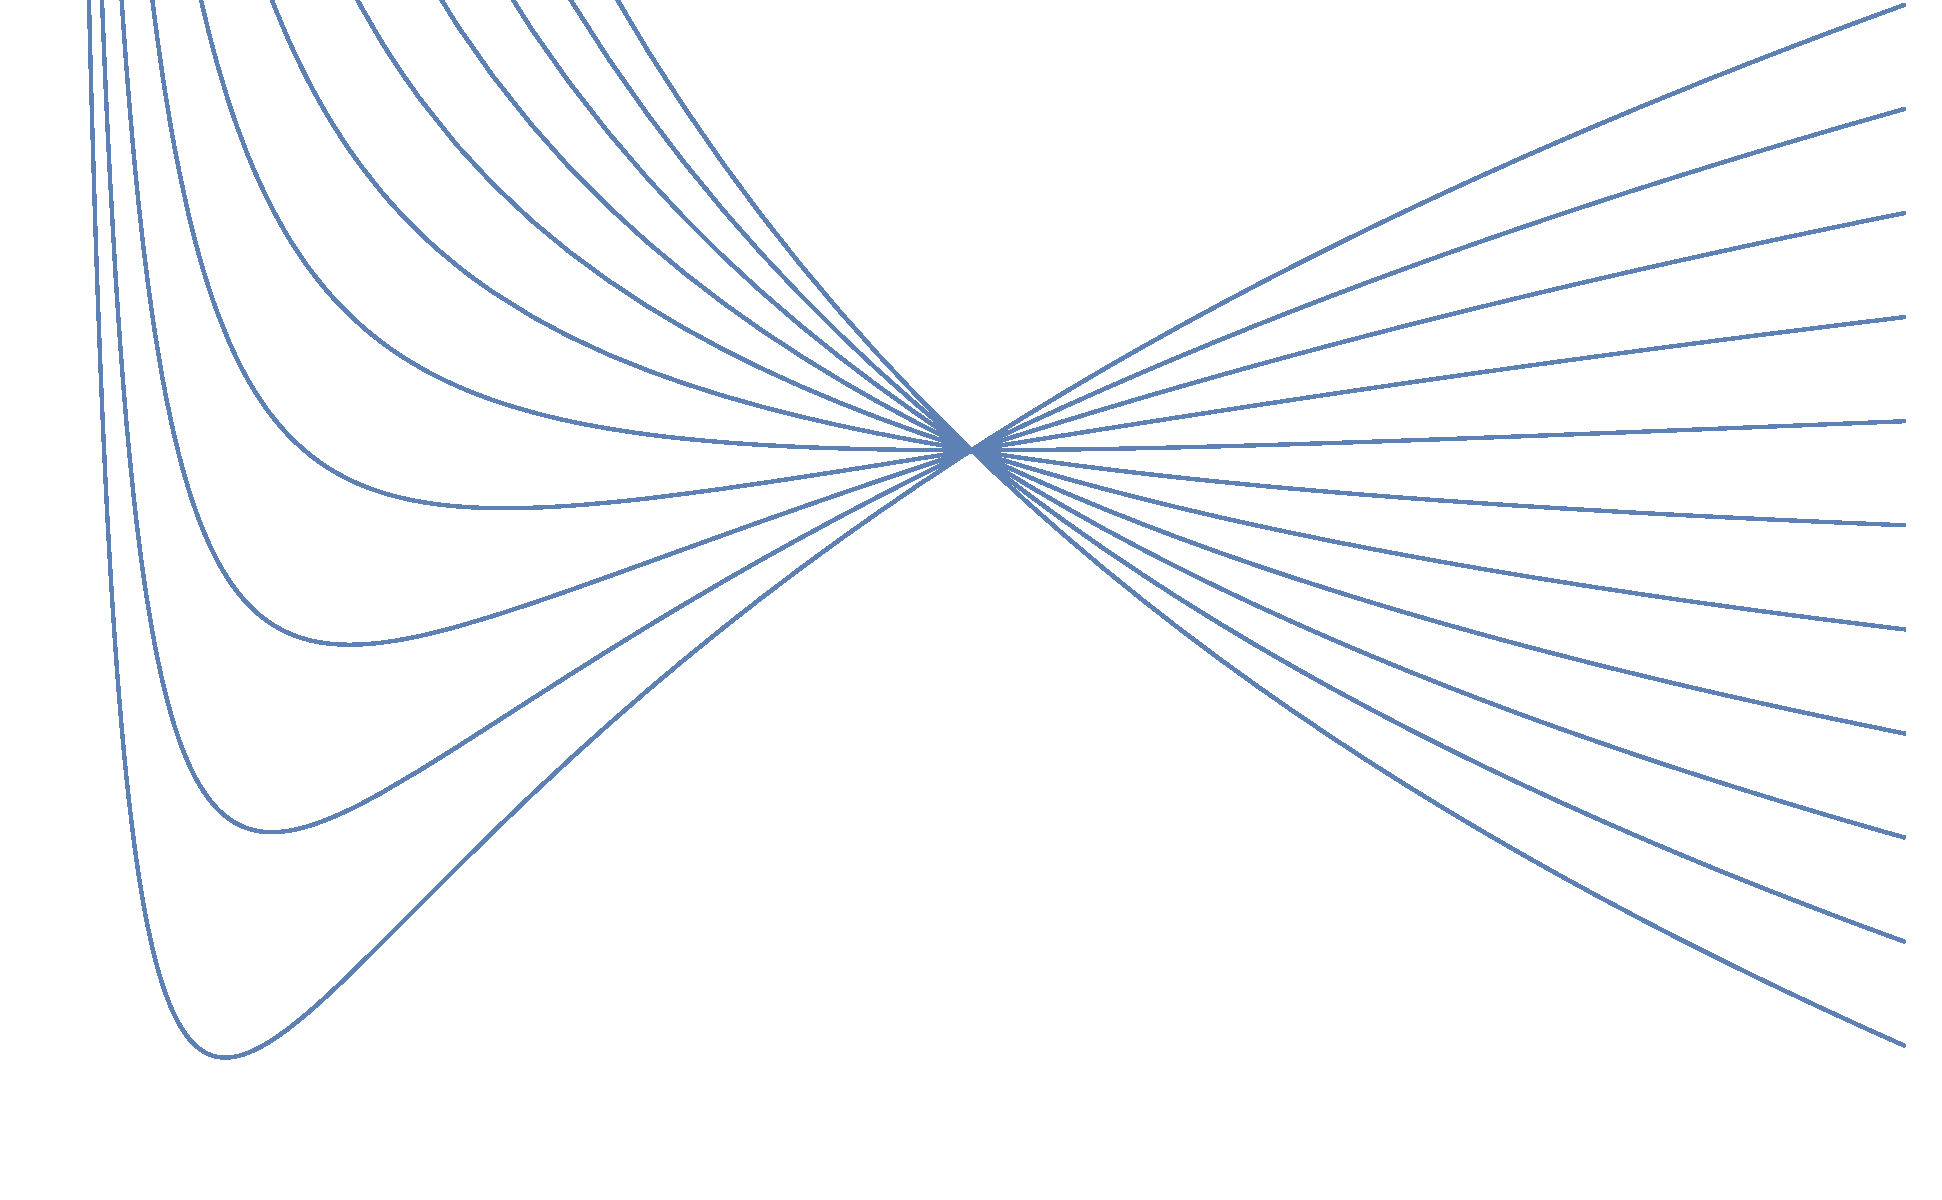
\includegraphics[scale=0.4]{../../Commun/Images/maths-cours-cauchy-3.pdf}};
\draw[->] (-6,0) -- (6.5,0) node[below] {$t$};
\draw[->] (-6,-4.2) -- (-6,4.2) node[left] {$y$};
\draw[shift={(0,0)}] (0pt,2pt) -- (0pt,-2pt) node[below] {1};
\draw[shift={(-6,1.1)}] (-2pt,0pt) -- (2pt,0pt) node[left] {1};
\end{tikzpicture}
\end{center}
  On peut aussi remarquer que pour $y_0\neq 1$, il n'existe aucune solution de cette équation différentielle
  vérifiant $y(1)=y_0$.
\end{remarqueUnique}

% \subsection{Méthode d'\nom{Euler}}

% On note $y$ la solution au problème de \nom{Cauchy}
% \[\begin{cases}
%   \forall t\in I \qsep y'(t)+a(t)y(t)=b(t)&\\
%   y(t_0)=y_0. &
%   \end{cases}\]
% Étant donnés $n\in\N$ et $\epsilon>0$ (supposé petit), la méthode d'Euler est
% une méthode permettant de calculer une valeur approchée
% de $u_n=y(t_0+n\epsilon)$. Comme $\epsilon$ est petit, l'approximation
% \[y'(t_0+n\epsilon)\approx
%   \frac{y(t_0+(n+1)\epsilon)-y(t_0+n\epsilon)}{\epsilon}=
%   \frac{u_{n+1}-u_n}{\epsilon}\]
% est raisonnable. $y$ étant solution de l'équation différentielle, on
% en déduit que
% \[y'(t_0+n\epsilon)+a(t_0+n\epsilon)y(t_0+n\epsilon)=b(t_0+n\epsilon)\]
% ce qui permet d'avoir une approximation de $u_{n+1}$ en fonction de $u_n$
% \[u_{n+1} \approx (1-\epsilon a(t_0+n\epsilon))u_n+\epsilon b(t_0+n\epsilon)\]
% Comme $u_0=y_0$, on calcule de proche en proche une valeur approchée de
% $u_n$.\\

% Par exemple, si $y$ est la solution au problème de \nom{Cauchy}
% \[\begin{cases}
%   \forall t\in \R \qsep y'(t)=y(t)&\\
%   y(0)=1 &
%   \end{cases}\]
% on sait que $y=\exp$.
% On se fixe $t>0$ et
% on souhaite calculer une valeur approchée de $y(t)$. Pour cela, on se donne
% $n\in\Ns$ et on pose $\epsilon=t/n$. On définit, pour tout $k\in\intere{0}{n}$,
% $u_k=y(k\epsilon)$. On a, d'après la méthode d'Euler
% \[u_0=1 \et \forall k\in\intere{0}{n-1} \qsep u_{k+1}\approx (1+\epsilon)u_k.\]
% Donc
% \[y(t)=u_n\approx (1+\epsilon)^n=\p{1+\frac{t}{n}}^n.\]
% On vérifie que lorsque $n$ tend vers $+\infty$, $(1+t/n)^n$ tend vers $\e^t$.
% Sur cet exemple, lorsque le pas $\epsilon$ tend vers $0$, la valeur approchée de
% $y(t)$, calculée par la méthode d'Euler, tend bien vers la valeur exacte de
% $y(t)$.

\section{Équation différentielle linéaire du second ordre}

\begin{definition}
Soit $a,b,c,d:I\to\K$ des fonctions définies sur un intervalle $I$. On appelle solution sur $I$ de l'équation différentielle linéaire du second ordre $ay''+by'+cy=d$, toute fonction $y:I\to\K$, dérivable deux fois sur $I$, telle que
\[\forall t\in I \qsep a(t)y''(t)+b(t)y'(t)+c(t)y(t)=d(t).\]
On dit que l'équation est \emph{résolue} lorsque $a$ ne s'annule pas et qu'elle est \emph{homogène} lorsque la fonction $d$ est nulle.
\end{definition}

\subsection{Équation différentielle homogène}

\begin{proposition}[utile=-3]
Soit $a,b,c\in\C$ avec $a\neq 0$ et $(E)$ l'équation différentielle
\[\forall t\in\R \qsep a y''(t)+by'(t)+cy(t)=0.\]
On résout sur $\C$ l'équation caractéristique $az^2+bz+c=0$.
\begin{itemize}
\item Si cette équation possède deux racines distinctes $r_1$ et $r_2$
  ($\Delta\neq 0$), alors les solutions complexes de $(E)$ sont les fonctions
  \[\dspappli{y_{\lambda,\mu}}{\R}{\C}{t}{\lambda \e^{r_1 t}+\mu \e^{r_2 t}}\]
  où $\lambda,\mu\in\C$.
\item Si cette équation admet une racine double $r$ ($\Delta=0$), alors les
  solutions complexes de $(E)$ sont les fonctions
  \[\dspappli{y_{\lambda,\mu}}{\R}{\C}{t}{\p{\lambda t+\mu}\e^{r t}}\]
  où $\lambda,\mu\in\C$.
\end{itemize}
\end{proposition}

\begin{preuve}
\begin{francois}
Soit $a, b, c\in\C$ avec $a\neq 0$. On considère l'équation différentielle
\[(E)\qquad \forall t\in\R \qsep a y''(t)+by'(t)+cy(t)=0.\]
On commence par chercher les solutions de $(E)$ qui sont de la forme $t\mapsto\e^{r t}$. Soit $r\in\C$ et $y$ la fonction de $\R$ dans $\C$ définie par
\[\forall t\in\R\qsep y(t)\defeq\e^{rt}.\]
D'après les théorèmes usuels, $y$ est dérivable deux fois sur $\R$ et
\begin{eqnarray*}
\forall t\in\R\qsep y'(t)&=&r\e^{rt}\\
y''(t)&=&r^2\e^{rt}.
\end{eqnarray*}
Donc
\begin{eqnarray*}
\text{$y$ est solution de $(E)$}
&\ssi& \forall t\in\R \qsep a y''(t)+by'(t)+cy(t)=0\\
&\ssi& \forall t\in \R\qsep (ar^2+br+c)\e^{rt}=0\\
&\ssi& ar^2+br+c=0.
\end{eqnarray*}
Puisqu'on est sur $\C$, cette équation $(E_c)$ admet au moins une solution $r_1\in\C$. La fonction $t\mapsto \e^{r_1 t}$ est donc une solution de $(E)$. Pour trouver l'ensemble des solutions de $(E)$, on va appliquer la méthode de la variation de la constante. Soit $y$ une fonction dérivable deux fois sur $\R$. On définit la fonction $u$ sur $\R$ par
\[\forall t\in\R\qsep u(t)\defeq y(t)\e^{-r_1 t}.\]
D'après les théorèmes usuels, $u$ est dérivable deux fois sur $\R$. De plus
\begin{eqnarray*}
\forall t\in\R\qsep y(t)&=&u(t)\e^{r_1 t}\\
y'(t)&=&\cro{u'(t)+r_1 u(t)}\e^{r_1 t}\\
y''(t)&=&\cro{u''(t)+2r_1 u'(t)+r_1^2 u(t)}\e^{r_1 t}.
\end{eqnarray*}
On en déduit que
\begin{eqnarray*}
\text{$y$ est solution de $(E)$}
&\ssi& \forall t\in\R \qsep a y''(t)+by'(t)+cy(t)=0\\
&\ssi& \forall t\in \R\qsep \cro{a u''(t)+\p{2ar_1+b}u'(t)+(ar_1^2+br_1+c)u(t)}\e^{r_1 t}=0\\
&\ssi& \forall t\in \R\qsep a u''(t)+\p{2ar_1+b}u'(t)+\underbrace{(ar_1^2+br_1+c)}_{=0}u(t)=0\\
&\ssi& \forall t\in \R\qsep a u''(t)+\p{2ar_1+b}u'(t)=0\\
&\ssi& \forall t\in \R\qsep u''(t)+\p{2r_1+\frac{b}{a}}u'(t)=0.
\end{eqnarray*}
On remarque que $y$ est une solution de $(E)$ si et seulement si $u'$ est solution d'une équation différentielle linéaire d'ordre 1 que l'on sait résoudre. La méthode de la variation de la constante nous a donc permis de faire baisser l'ordre de l'équation différentielle.
\begin{itemize}
\item Si l'équation caractéristique $(E_c)$ admet deux racines distinctes $r_1$ et $r_2$. Alors, les relations coefficients racines, donnent
\[r_1+r_2=-\frac{b}{a}\]
donc
\begin{eqnarray*}
\text{$y$ est solution de $(E)$}
&\ssi& \forall t\in \R\qsep u''(t)+\p{r_1-r_2}u'(t)=0\\
&\ssi& \forall t\in \R\qsep u''(t)\e^{(r_1-r_2)t}+\p{r_1-r_2}u'(t)\e^{(r_1-r_2)t}=0\\
&\ssi& \forall t\in\R\qsep \frac{{\rm d}}{{\rm d}t}\p{u'(t)\e^{(r_1-r_2)t}}=0\\
&\ssi& \exists\lambda\in\C\qsep \forall t\in\R\qsep u'(t)\e^{(r_1-r_2)t}=\lambda\\
&\ssi& \exists\lambda\in\C\qsep \forall t\in\R\qsep u'(t)=\lambda \e^{(r_2-r_1)t}\\
&\ssi& \exists\lambda,\mu\in\C\qsep \forall t\in\R\qsep u(t)=\frac{\lambda}{r_2-r_1} \e^{(r_2-r_1)t}+\mu\\
&\ssi& \exists\lambda,\mu\in\C\qsep \forall t\in\R\qsep u(t)=\mu+\lambda \e^{(r_2-r_1)t}\\
&\ssi& \exists\lambda,\mu\in\C\qsep \forall t\in\R\qsep y(t)\e^{-r_1 t}=\mu+\lambda \e^{(r_2-r_1)t}\\
&\ssi& \exists\lambda,\mu\in\C\qsep \forall t\in\R\qsep y(t)=\mu \e^{r_1 t}+\lambda \e^{r_2 t }.
\end{eqnarray*}
Les solutions de $(E)$ sont donc les fonctions
\[\dspappli{y_{\lambda,\mu}}{\R}{\C}{t}{\lambda \e^{r_1 t}+\mu \e^{r_2 t}}\]
où $\lambda,\mu\in\C$.
\item Si l'équation caractéristique $(E_c)$ admet une unique racine, les relations coefficients racines donnent
\[2r_1=-\frac{b}{a}\]
donc
\begin{eqnarray*}
\text{$y$ est solution de $(E)$}
&\ssi& \forall t\in \R\qsep u''(t)=0\\
&\ssi& \exists\lambda\in\C\qsep \forall t\in \R\qsep u'(t)=\lambda\\
&\ssi& \exists\lambda,\mu\in\C\qsep \forall t\in \R\qsep u(t)=\lambda t+\mu\\
&\ssi& \exists\lambda,\mu\in\C\qsep \forall t\in\R\qsep y(t)\e^{-r_1 t}=\lambda t+\mu\\
&\ssi& \exists\lambda,\mu\in\C\qsep \forall t\in\R\qsep y(t)=(\lambda t+\mu) \e^{r_1 t}
\end{eqnarray*}
Les solutions de $(E)$ sont donc les fonctions
\[\dspappli{y_{\lambda,\mu}}{\R}{\C}{t}{(\lambda t+\mu)\e^{r_1 t}}\]
où $\lambda,\mu\in\C$.
\end{itemize}
\end{francois}
\begin{victor}
\begin{itemize}
\item [$\bullet$] Cherchons d'abord des solutions exponentielles de $(E)$. Soit $r\in \C$. Définissons $\dspappli{u}{\R}{\C}{t}{\e^{rt}}$.
\begin{eqnarray*}
u \in \mathcal{S}(E) &\Longleftrightarrow& \forall t\in \R, (ar^2+br+c)\e^{rt}=0\\
&\Longleftrightarrow& \forall x\in \R, (ar^2+br+c)=0
\end{eqnarray*}
\item [$\bullet$] \underline{Méthode de l'abaissement de l'ordre :}

Supposons que l'on dispose de $r\in\C$ une racine de $(EC)$. \underline{Principe de la méthode :} chercher des solutions de $(E)$ sous la forme $x\mapsto \e^{rt}v(t)$.

Soit $u:\R\to \K$ deux fois dérivables. Définissons $\dspappli{v}{\R}{\C}{t}{\e^{-rt}u(t)}$. $v$ est deux fois dérivables sur $\R$ et $\forall x\in\R$ :
\[u'(t)=\p{rv(t)+v'(t)}\e^{rt}\]
\[u''(t)=\p{v''(t)+2rv'(t)+r^2v(t)}\e^{rt}\]

Ainsi,
\begin{eqnarray*}
u\in \mathcal{S}(E)&\Longleftrightarrow & \forall t\in \R, au''(t)+bu'(t)+cu(t)=0\\
&\Longleftrightarrow & \forall t\in \R, v''(t)\p{a\e^{rt}}+v'(t)\p{2ar\e^{rt}+b\e^{rt}}+v(t)\p{ar^2\e^{rt}+br\e^{rt}+c\e^{rt}}=0\\
&\Longleftrightarrow & \forall t\in \R, av''(t)+\p{2ar+b}v'(t)+\p{ar^2+br+c}v(t)=0\\
&\Longleftrightarrow & \forall t\in \R, av''(t)+\p{2ar+b}v'(t)=0\\
&\Longleftrightarrow & v' \text{ est solution de } (E') : y'+\p{2r+\dfrac{b}{a}}y=0
\end{eqnarray*}
La solution générale de $(E')$ est : $t\mapsto \lambda \e^{-\p{2r+\dfrac{b}{a}}t}$. On est alors amené à distinguer deux cas pour la primitive :

\item [$\bullet$] \underline{Premier cas : } $2r+\dfrac{b}{a}=0$, i.e $r=\dfrac{-b}{2a}$. \textbf{C'est le cas où le discriminant de l'EC est nul.}
\begin{eqnarray*}
u\in \mathcal{S}(E)&\Longleftrightarrow & \exists \lambda\in\K \text{ tel que } \forall t \in \R, v'(t)=\lambda\\
&\Longleftrightarrow & \exists (\lambda,\mu)\in\K^2 \text{ tel que } \forall t \in \R, v(t)=\lambda t+\mu\\
&\Longleftrightarrow & \exists (\lambda,\mu)\in\K^2 \text{ tel que } \forall t \in \R, u(t)=(\lambda t+\mu)\e^{rt}
\end{eqnarray*}

\item [$\bullet$] \underline{Deuxième cas : } Lorsque le discriminant de l'EC est non nul. Notons $r'$ la seconde racine de l'EC. Alors, par exemple, avec $\delta$ une racine du discriminant dans $\C$ :
\[r=\dfrac{-b+\delta}{2a} \quad ; \quad r'=\dfrac{-b-\delta}{2a}\]
Ainsi, $-\p{2r+\dfrac{b}{a}}=r'-r$. D'où :
\begin{eqnarray*}
u\in \mathcal{S}(E)&\Longleftrightarrow & \exists \lambda\in\K \text{ tel que } \forall t \in \R, v'(t)=\lambda\e^{(r'-r)t}\\
&\Longleftrightarrow & \exists (\lambda,\mu)\in\K^2 \text{ tel que } \forall t \in \R, v(t)=\frac{\lambda}{r'-r}\e^{(r'-r)t}+\mu\\
&\Longleftrightarrow & \exists (\lambda,\mu)\in\K^2 \text{ tel que } \forall t \in \R, u(t)=\frac{\lambda}{r'-r}\e^{r't}+\mu\e^{rt}\\
&\Longleftrightarrow & \exists (\lambda,\mu)\in\K^2 \text{ tel que } \forall t \in \R, u(t)=\lambda\e^{r't}+\mu\e^{rt} \text{ quitte à changer }\lambda.
\end{eqnarray*}
\end{itemize}
\end{victor}
\end{preuve}

% \begin{remarques}
% \remarque L'ensemble des solutions complexes de cette équation différentielle
%   est un \Cev de dimension 2.
% \end{remarques}

\begin{exoUnique}
\exo Résoudre l'équation différentielle $y''-3y'+2y=0$.
\end{exoUnique}

\begin{proposition}[utile=-3]
Soit $a,b,c\in\R$ avec $a\neq 0$ et $(E)$ l'équation différentielle
\[\forall t\in\R \qsep a y''(t)+by'(t)+cy(t)=0.\]
On résout sur $\C$ l'équation caractéristique $az^2+bz+c=0$.
\begin{itemize}
\item Si cette équation possède deux racines réelles distinctes $r_1$ et $r_2$
  ($\Delta> 0$), alors les solutions réelles de $(E)$ sont les fonctions
  \[\dspappli{y_{\lambda,\mu}}{\R}{\R}{t}{\lambda \e^{r_1 t}+\mu \e^{r_2 t}}\]
  où $\lambda,\mu\in\R$.
\item Si cette équation admet une racine double $r$ ($\Delta=0$), alors les
  solutions réelles de $(E)$ sont les fonctions
  \[\dspappli{y_{\lambda,\mu}}{\R}{\R}{t}{\p{\lambda t+\mu}\e^{r t}}\]
  où $\lambda,\mu\in\R$.
\item Si cette équation admet deux racines complexes conjuguées $r+\ii\omega$ et
  $r-\ii\omega$ ($\Delta <0$), alors les solutions réelles de $(E)$ sont les
  fonctions
  \[\dspappli{y_{\lambda,\mu}}{\R}{\R}{t}{\cro{\lambda\cos\p{\omega t}+
    \mu\sin\p{\omega t}}\e^{r t}}\]
  où $\lambda,\mu\in\R$.
\end{itemize}
\end{proposition}

\begin{preuve}
\begin{francois}
Soit $a,b,c\in\R$ avec $a\neq 0$. On considère l'équation différentielle
\[(E)\qquad\forall t\in\R \qsep a y''(t)+by'(t)+cy(t)=0\]
ainsi que son équation caractéristique associée $(E_c)$~: $az^2+bz+c=0$.
\begin{itemize}
\item Si $\Delta>0$ ou $\Delta=0$, l'équation caractéristique admet au moins une solution réelle $r_1$. La démonstration faite dans le cas de la recherche des solutions complexes s'adapte simplement et permet de trouver l'ensemble des solutions réelles de $(E)$.
\item Si $\Delta<0$, l'équation caractéristique admet deux solutions complexes conjuguées $r+\ii\omega$ et $r-\ii\omega$. Montrons que les solutions réelles de $(E)$ sont les fonctions
\[t\mapsto \cro{\lambda\cos\p{\omega t}+\mu\sin\p{\omega t}}\e^{r t}\]
où $\lambda,\mu\in\R$.
\begin{itemize}
\item Ce sont des solutions de $(E)$. En effet, soit $\lambda,\mu\in\R$ et $y$ la fonction définie sur $\R$ par
\[\forall t\in\R\qsep y(t)\defeq \cro{\lambda\cos\p{\omega t}+\mu\sin\p{\omega t}}\e^{r t}.\]
Alors
\begin{eqnarray*}
\forall t\in\R\qsep y(t)
&=& \cro{\lambda\cos\p{\omega t}+\mu\sin\p{\omega t}}\e^{r t}\\
&=& \cro{\lambda\frac{\e^{\ii\omega t}+\e^{-\ii\omega t}}{2}+\mu\frac{\e^{\ii\omega t}-\e^{-\ii\omega t}}{2\ii}}\e^{r t}\\
&=& \underbrace{\p{\frac{\lambda}{2}+\frac{\mu}{2\ii}}}_{\eqdef \alpha\in\C}\e^{(r+\ii\omega)t}+\underbrace{\p{\frac{\lambda}{2}-\frac{\mu}{2\ii}}}_{\eqdef \beta\in\C}\e^{(r-\ii\omega)t}.
\end{eqnarray*}
D'après la proposition précédente, on en déduit que $y$ est une solution de $(E)$.
\item Ce sont les seules solutions réelles de $(E)$. En effet, soit $y$ une solution réelle de $(E)$. Alors, c'est une solution complexe, donc d'après la proposition précédente, il existe $\lambda,\mu\in\C$ tels que
\[\forall t\in\R\qsep y(t)=\lambda\e^{(r+\ii\omega)t}+\mu\e^{(r-\ii\omega)t}.\]
Il existe $\alpha,\beta,\gamma,\delta\in\R$ tels que $\lambda=\alpha+\ii\beta$ et $\mu=\gamma-\ii\delta$. Alors
\begin{eqnarray*}
\forall t\in\R\qsep y(t)
&=& \Re\cro{y(t)}\quad\text{car $y$ est réelle}\\
&=& \Re\cro{\p{\alpha+\ii\beta}\e^{(r+\ii\omega)t}+\p{\gamma+\ii\delta}\e^{(r-\ii\omega)t}}\\
&=& \Re\cro{\p{\alpha+\ii\beta}\p{\cos(\omega t)+\ii\sin(\omega t)}+\p{\gamma+\ii\delta}\p{\cos(\omega t)-\ii\sin(\omega t)}}\e^{rt}\\
&=& [\underbrace{(\alpha+\gamma)}_{\eqdef \lambda'\in\R}\cos(\omega t)+\underbrace{(\gamma-\beta)}_{\eqdef \mu'\in\R}\sin(\omega t)]\e^{rt}
\end{eqnarray*}
donc $y$ est bien de la forme demandée.
\end{itemize}
\end{itemize}
\end{francois}
\begin{victor}
Les deux premiers cas sont une conséquence de la proposition précédente. Il reste donc à traiter le cas où $\Delta<0$.

L'EC admet alors deux racines $r\pm i\omega$. 

\underline{Analyse :} Soit $y:\R\to\R$ une solution de $(E)$. D'après la proposition précédente, on peut fixer $(A,B)\in \C^2$ tels que \[\forall t\in\R, y(t)=A\e^{(r+i\omega)t}+B\e^{(r-i\omega)t}=\e^{rt}\p{A\e^{i\omega t}+B\e^{-i\omega t}}.\]
Or, $\forall t\in\R, y(t)=\Re(y(t))=\e^{rt}\Re\p{A\e^{i\omega t}+B\e^{-i\omega t}}$ qui est donc de la forme $y(t)=\cro{c_1\cos\p{\omega t}+c_2\sin\p{\omega t}}\e^{r t}$.

\underline{Synthèse :} Réciproquement, soit $(c_1,c_2)\in\R^2$. Définissons $\dspappli{y}{\R}{\R}{t}{\cro{c_1\cos\p{\omega t}+c_2\sin\p{\omega t}}\e^{r t}}$.
On applique les formules d'Euler pour s'apercevoir que $y$ ainsi définie est bien solution de $(E)$ car de la forme des solutions de la proposition précédente.
\end{victor}
\end{preuve}

\begin{remarqueUnique}
% \remarque L'ensemble des solutions réelles de cette équation différentielle
%   est un \Rev de dimension 2.
\remarque Dans le cas où l'équation caractéristique admet deux racines complexes
  conjuguées, les solutions de $(E)$ peuvent s'écrire sous la forme
  \[\dspappli{y_{\lambda,\phi}}{\R}{\R}{t}{\lambda \sin\p{\omega t-\phi}\e^{r t}}\]
  où $\lambda,\phi\in\R$. Lors de la recherche effective de tels coefficients, 
  quitte à changer $\phi$ en $\phi+\pi$, on impose souvent $\lambda\in\RP$.
% \remarque Étant donnés $t_0\in\R$ et $y_0,y_1\in\R$, on appelle problème de
%   \nom{Cauchy} la recherche des solutions $y$ de l'équation différentielle
%   $ay''+by'+cy=0$ telles que $y(t_0)=y_0$ et $y'(t_0)=y_1$. On peut montrer
%   que tout problème de \nom{Cauchy} admet une et une seule solution.
\end{remarqueUnique}

\begin{exos}
\exo Résoudre l'équation différentielle $y''+2y'+2y=0$.
\exo Soit $\omega_0\in\R$. Résoudre l'équation différentielle
  $y''+\omega_0^2 y=0$.
\exo En effectuant le changement de fonction inconnue $z(t)= t^2 y(t)$,
  résoudre l'équation différentielle
  \[\forall t\in\RPs \qsep t^2 y''(t)+4ty'(t)+(2-t^2)y(t)=0.\]
  \begin{sol}
  On trouve $z''-z=0$. Donc $y(t)=(ae^t+be^{-t})/t^2$.
  \end{sol}
\exo En effectuant le changement de variable $t=\sqrt{u}$, résoudre
  l'équation différentielle
  \[\forall t\in\RPs \qsep ty''(t)-y'(t)+4t^3y(t)=0.\]
  \begin{sol}
  On définit la fonction $z$ sur $\RPs$ par $z(u)=y(\sqrt{u})$, donc
  $y(t)=z(t^2)$. L'équation devient alors $z''+z=0$. Les solutions sont donc
  les $y(t)=c_1\cos(t^2)+c_2\sin(t^2)$.
  \end{sol}
\end{exos}

\subsection{Équation différentielle avec second membre}

\begin{proposition}[utile=-3,nom={Théorème de superposition}]
Soit $a,b,c,d:I\to\K$ des fonctions définies sur un intervalle $I$.
Si $y_p$ est une solution \og particulière \fg de l'équation différentielle
\[\forall t\in\R \qsep a(t)y''(t)+b(t)y'(t)+c(t)y(t)=d(t)\]
alors les solutions de cette équation différentielle sont les fonctions $y_p+y$
où $y$ parcourt l'ensemble des solutions de l'équation différentielle homogène
associée
\[\forall t\in\R \qsep a(t)y''(t)+b(t)y'(t)+c(t)y(t)=0.\]
\end{proposition}


\begin{proposition}[utile=-3,nom={Théorème de superposition}]
\begin{itemize}
\item Soit $a,b,c,d_1,d_2:I\to\K$ des fonctions définies sur un intervalle $I$, $\lambda,\mu\in\K$ et $y_{p_1},y_{p_2}:I\to\K$ des solutions \og particulières \fg des équations
  différentielles respectives $ay''+by'+cy=d_1$ et $ay''+by'+cy=d_2$. Alors
  $\lambda y_{p_1}+\mu y_{p_2}$ est une solution \og particulière \fg de l'équation différentielle
  \[\forall t\in\R \qsep a(t)y''(t)+b(t)y'(t)+c(t)y(t)=
    \lambda d_1(t)+\mu d_2(t).\]
\item Soit $a,b,c:I\to\R$ et $d:I\to\C$ des fonctions définies sur un intervalle $I$ et $y_p:I\to\C$ une solution
  \og particulière \fg de l'équation différentielle $ay''+by'+cy=d$. Alors
  $\Re(y_p)$ est une solution \og particulière \fg de l'équation différentielle
  \[\forall t\in \R \qsep a(t)y''(t)+b(t)y'(t)+c(t)y(t)=\Re(d(t)).\]
\end{itemize}
\end{proposition}

\begin{remarqueUnique}
\remarque Bien entendu, une proposition similaire existe pour la partie imaginaire.
\end{remarqueUnique}

\begin{proposition}[utile=-3]
Soit $a,b,c\in\C$ avec $a\neq 0$. Si $P$ est un polynôme de degré $n$ et
$\alpha\in\C$, alors l'équation différentielle
\[\forall t\in \R \qsep ay''(t)+by'(t)+cy(t)=P(t)\e^{\alpha t}\]
admet comme solution une (unique) fonction du type
$t\mapsto t^m Q(t)\e^{\alpha t}$ où $Q$ est un polynôme de degré $n$ et
$m$ est l'ordre de $\alpha$ comme racine de l'équation
caractéristique (avec par convention $m=0$ si $\alpha$ n'est pas racine
de cette équation).
\end{proposition}

\begin{exos}
\exo Déterminer les solutions de l'équation différentielle
  $y''(t)+y'(t)+y(t)=t^2$.
  \begin{sol}
  Les solutions sont les
  \[y(x)=\p{c_1\sin\p{\frac{\sqrt{3}}{2}c}+c_2\cos\p{\frac{\sqrt{3}}{2}c}}
    e^{-\frac{x}{2}}+x^2-2x\]
  \end{sol}
\exo Déterminer les solutions de l'équation différentielle
  $y''(t)+y(t)=t\cos t$.
  \begin{sol}
  On trouve
  \[\frac{1}{4}(-it^2+t)e^{it}\]
  puis
  \[\frac{1}{4}\p{t\cos t+t^2\sin t}\]
  \end{sol}
\end{exos}

\subsection{Problème de \nom{Cauchy}}

\begin{definition}[nom={Problème de \nom{Cauchy}}]
Soit $a,b,c,d:I\to\K$ des fonctions définies sur un intervalle $I$, $t_0\in I$ et
$y_0,y_1\in\K$. On appelle \emph{problème de \nom{Cauchy}} la recherche des solutions $y$ de
l'équation différentielle du second ordre
\[\forall t\in I \qsep a(t)y''(t)+b(t)y'(t)+c(t)y(t)=d(t)\]
telles que $y(t_0)=y_0$ et $y'(t_0)=y_1$.
\end{definition}

\begin{theoreme}[nom={Théorème de \nom{Cauchy-Lipschitz}}]
Soit $a,b,c:I\to\K$ des fonctions continues sur un intervalle $I$,
$t_0\in I$ et $y_0,y_1\in\K$. Alors il existe une et une seule solution à
l'équation différentielle résolue du second ordre
\[\forall t\in I \qsep y''(t)+a(t)y'(t)+b(t)y(t)=c(t)\]
telle que $y(t_0)=y_0$ et $y'(t_0)=y_1$.
\end{theoreme}

\begin{remarques}
\remarque Graphiquement, cette proposition signifie que par tout
  point $(t_0,y_0)\in I\times \R$ passe un et un seul graphe de pente $y_1\in\R$,
  solution de l'équation différentielle $y''(t)+a(t)y'(t)+b(t)y(t)=c(t)$. Les courbes intégrales peuvent se croiser, mais doivent avoir des pentes différentes lorsqu'elles se croisent. Par exemple, voici quelques
  solutions de l'équation différentielle
  \[\forall t\in\R\qsep y''(t)+y(t)=\frac{1}{2}t^2+t.\]
\begin{center}
\begin{tikzpicture}[>=latex]
\node at (0,0) {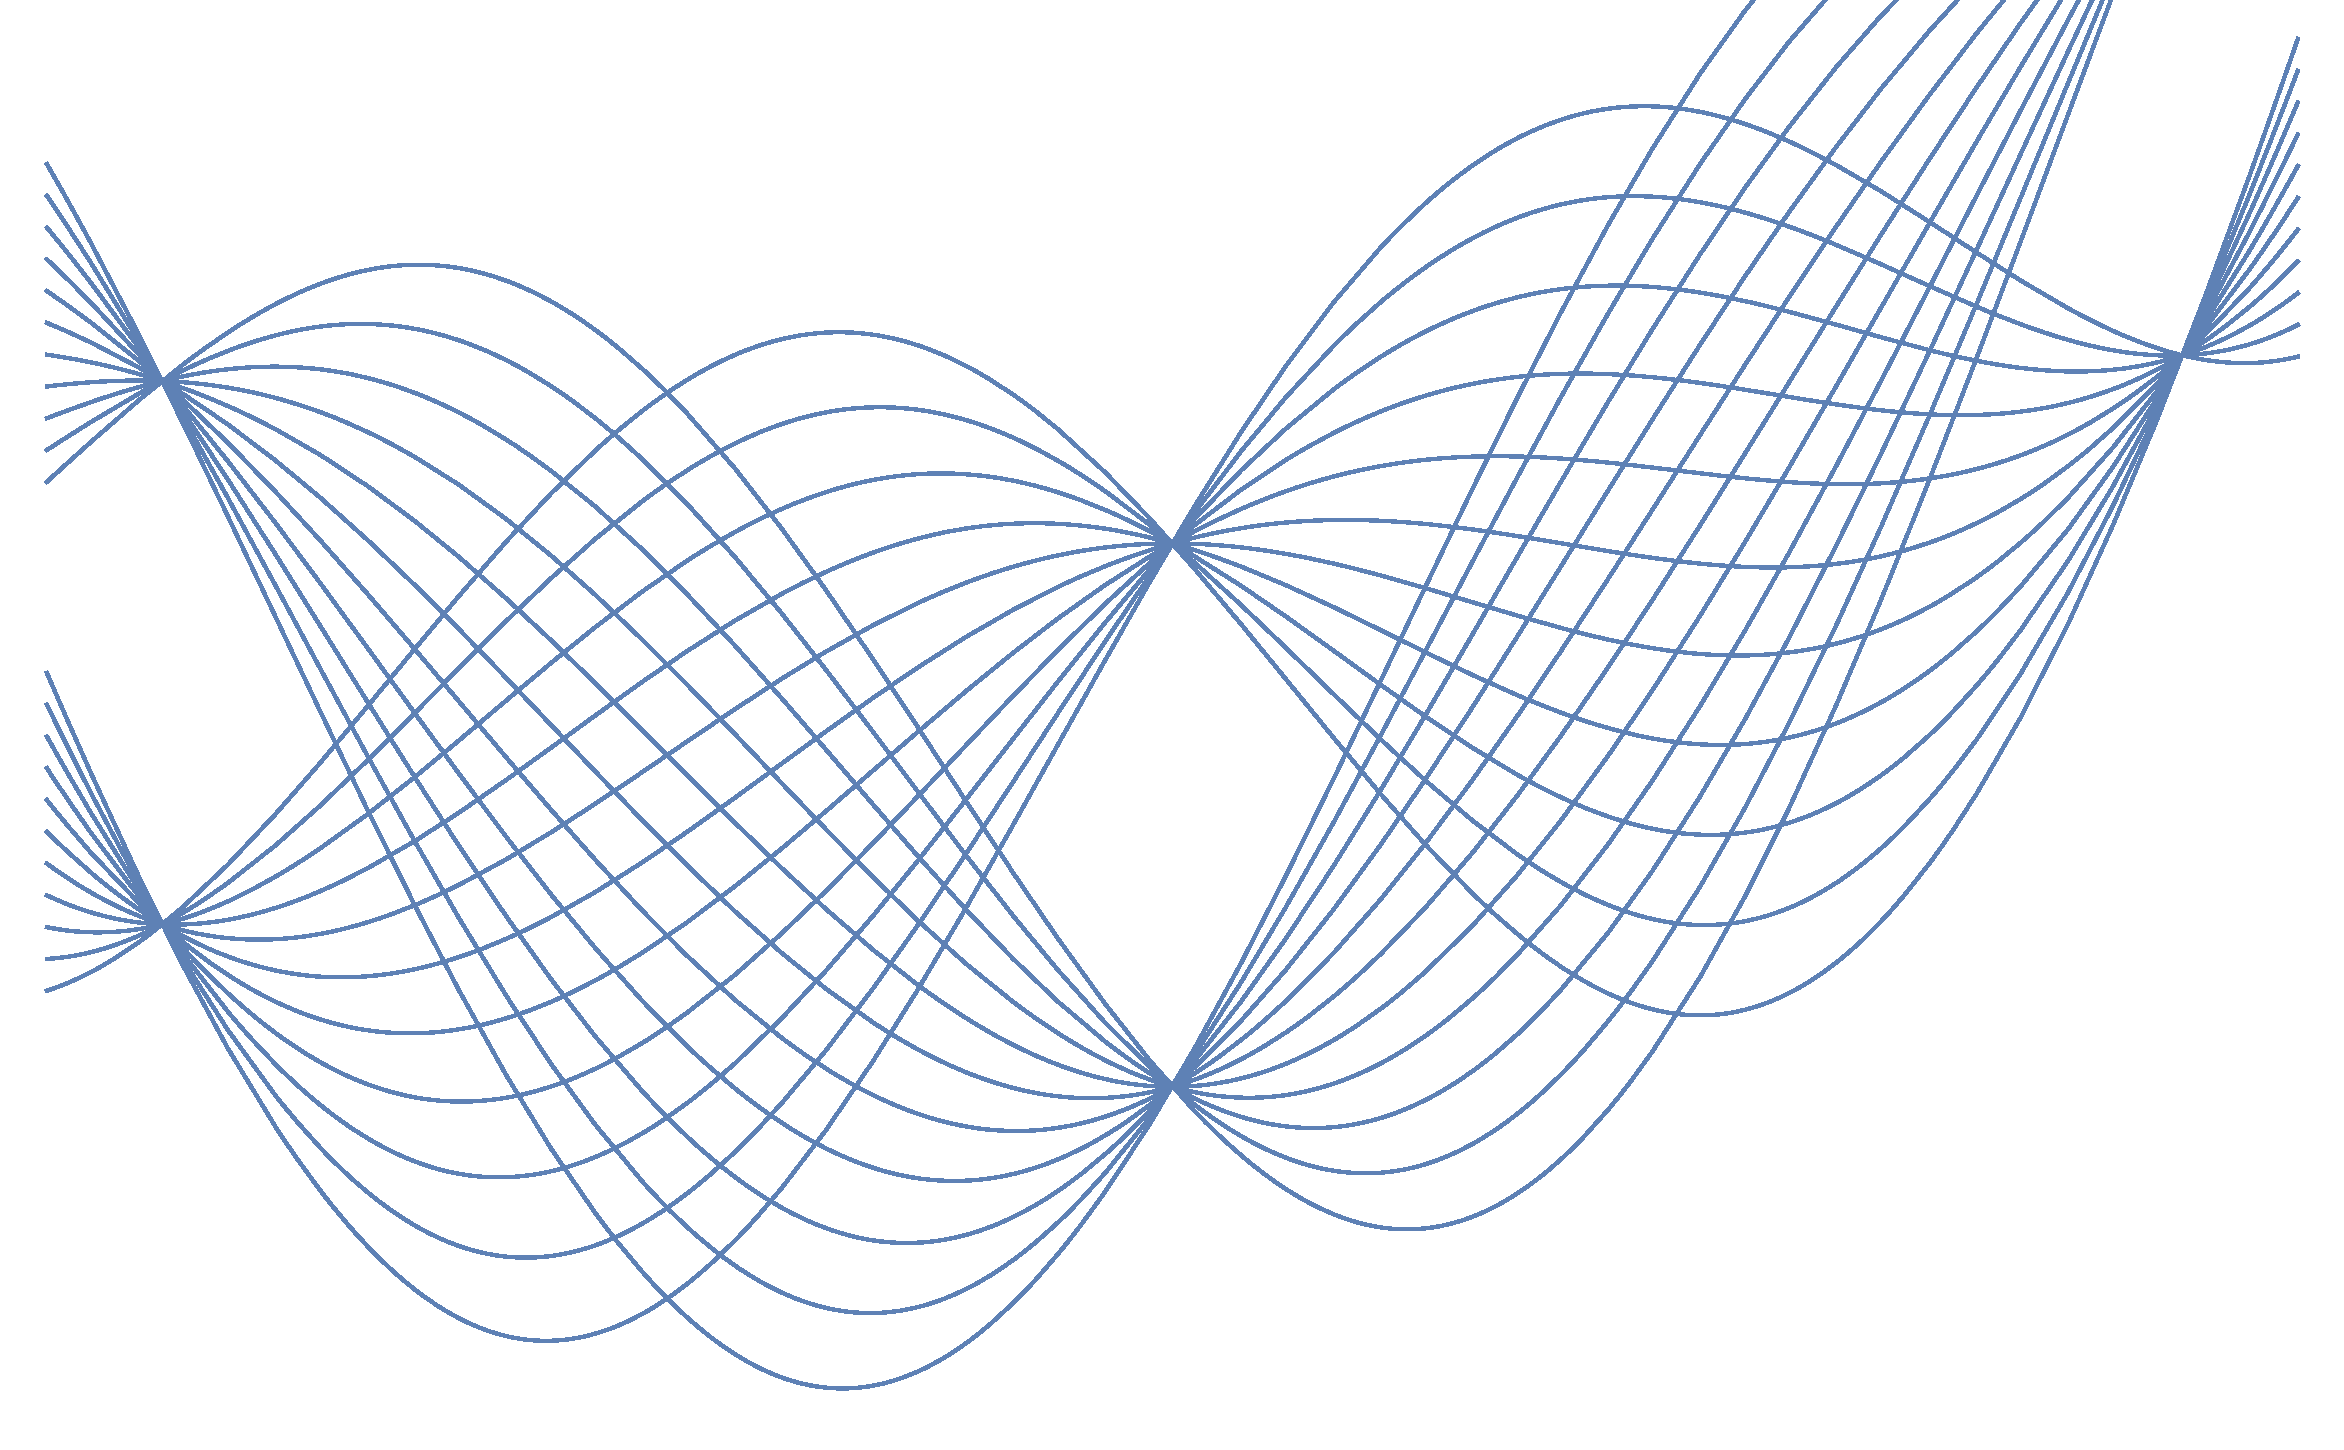
\includegraphics[scale=0.4]{../../Commun/Images/maths-cours-cauchy-2.pdf}};
\draw[->] (-7.65,0) -- (7.65,0) node[below] {$t$};
\draw[->] (0,-5) -- (0,5) node[left] {$y$};
\end{tikzpicture}
\end{center}
\remarque Le théorème de \nom{Cauchy-Lipschitz} prouve que la connaissance de la valeur de $y$ et de sa dérivée à l'instant $t_0$ d'un système régi par une équation différentielle résolue du second ordre permet de connaitre complètement son passé et son futur.
\end{remarques}
\vspace{2ex}
\begin{exoUnique}
\exo Résoudre le problème de \nom{Cauchy}
  \[y(0)=0,\quad y'(0)=1,\et \forall t\in\R\qsep y''(t)+y(t)=\frac{1}{2}t^2+t.\]
\begin{sol}
On trouve $y(t)=\frac{1}{2}t^2+t-1+\cos(t)$.
\end{sol}
\end{exoUnique}
%END_BOOK

\end{document}
\section{Exercices}
\setcounter{numeroexercice}{1}
\documentclass{magnolia}


\magtex{tex_driver={pdftex}}
\magfiche{document_nom={Exercices sur les équations différentielles},
          auteur_nom={François Fayard},
          auteur_mail={fayard.prof@gmail.com}}
\magexos{exos_matiere={maths},
         exos_niveau={mpsi},
         exos_chapitre_numero={6},
         exos_theme={Équations différentielles}}
\magmisenpage{}
\maglieudiff{}
\magprocess

\begin{document}

%BEGIN_BOOK
\magsection{Équation différentielle linéaire du premier ordre}
% \magsubsection{Équation différentielle homogène}

% \exercice{nom={Équation de \nom{Bernoulli}}}
% Soit $\alpha>0$. On considère l'équation différentielle
% \[\forall t\in\interfo{\alpha}{+\infty} \qsep t^2y'(t)+y(t)+y^2(t)=0.\]
% On admet que l'unique solution s'annulant de cette équation est la fonction nulle. En effectuant le changement de fonction $z=1/y$, déterminer l'ensemble des solutions de $(E)$.

% \begin{sol}
% Les solutions sont la fonction nulle, les fonctions
% \[\forall t\geq\alpha\qsep y(t)=\frac{-1}{c\e^{-\frac{1}{t}}+1}\]
% où $c\geq 0$, ainsi que les fonctions
% \[\forall t\geq\alpha\qsep y(t)=\frac{1}{c\e^{-\frac{1}{t}}-1}\]
% où $c> \e^{1/\alpha}$.
% On doit utiliser le Théorème de Cauchy-Lipschitz (version non donné aux élèves ?). Si $y$ s'annule alors, c'est la fonction nulle. Sinon, $y$ ne s'annule jamais et on peut alors poser $z=y^{1-n}$. On a alors $z'=(1-n)y'y^{-n}$. Et en en divisant $(E)$ par $y^n$, on a alors $(E) \Longleftrightarrow t^2\dfrac{z'}{1-n}+z+1=0$.

% Disons pour simplifier que $I$ ne contient pas $0$, en résolvant cette équation différentielle, on obtient $z(t)=\lambda e^{\frac{1-n}{t}}-1$. Ainsi, $y(t)=\p{\lambda e^{\frac{1-n}{t}}-1}^{\frac{1}{1-n}}$.

% Quand j'essaie de vérifier qu'un tel $y$ fonctionne, ça ne marche pas...
% \end{sol}


\magsubsection{Équation différentielle avec second membre}


\exercice{nom={Calcul}}
Résoudre les équations différentielles suivantes sur un intervalle à préciser
\[\textbf{a.}\ y'+2y=x^2-2x+3, \qquad
%%\question $\p{x\ln x}y'-y=-\frac{\ln x+1}{x}$
\textbf{b.}\ \p{1+x}y'+y=1+\ln (1+x),\]
\[\textbf{c.}\ y'+y=\frac{1}{1+\e^x}.\]
%, \qquad y'=\sqrt{1+y^2}.\]
%%\question $2xy'+y=x^n \quad n\in\N$
\begin{sol}
\begin{questions}
\question Soit $(E)$ l'équation différentielle
 \[(E) \quad \forall x\in\R\qsep y'(x)+2y(x)=x^2-2x+3\]
 On cherche une solution particulière de $(E)$ sous la forme $y(x)=ax^2+bx+c$. Soit $a, b, c\in\R$ et $y$ la fonction définie sur $\R$ par
 \[\forall x\in\R \qsep y(x)\defeq ax^2+bx+c\]
 D'après les théorèmes usuels, $y$ est dérivable sur $\R$ et
\[\forall x\in\R\qsep y'(x)= 2ax+b.\]
donc
\begin{eqnarray*}
\text{$y$ est solution de $(E)$}
&\ssi& \forall x\in\R\qsep y'(x)+2y(x)=x^2-2x+3\\
&\ssi& \forall x\in\R\qsep 2ax^2+(2b+2a)x+(2c+b)=x^2-2x+3\\
&\ssi& 2a = 1 \et 2a+2b=-2 \et b+2c=3\\
&    & \text{car un polynôme admettant une infinité de racines est nul}\\
&\ssi& a = \frac{1}{2} \et b=-\frac{3}{2} \et c=\frac{9}{4}.
\end{eqnarray*}
Donc
\[x\mapsto \frac{1}{2}x^2-\frac{3}{2}x+\frac{9}{4}\]
est une solution particulière de $(E)$. De plus, les solutions de l'équation différentielle homogène associée
\[(E_H) \quad \forall x\in\R\qsep y'(x)+2y(x)=0\]
sont les fonctions $x\mapsto \lambda\e^{-2x}$ où $\lambda\in\R$. Les solutions de $(E)$ sont donc les fonctions
\[x\mapsto \lambda\e^{-2x}+\frac{1}{2}x^2-\frac{3}{2}x+\frac{9}{4}\]
où $\lambda\in\R$.
\question $y(x)=\ln(1+x)+c/(1+x)$.
\question $y(x)=\cro{\ln(1+e^x)+c}e^{-x}$.
\question $y(x)=\sh(x+c)$.
\end{questions}
\end{sol}

\exercice{nom={Avec un second membre}}
Déterminer les fonctions dérivables $y:\R\to\R$ telles que
\[\forall x\in\R\qsep y'(x)+y(x)=\integ{0}{1}{y(t)}{t}.\]

\exercice{nom={Équations fonctionnelles}}
\begin{questions}
\question Déterminer les fonctions dérivables $f:\R\to\R$ telles que
\[\forall x,y\in\R\qsep f(x+y)=\e^x f(y)+f(x)\e^y.\]
\question Déterminer les fonctions dérivables $f:\R\to\R$ telles que $f(0)\neq 0$ et
\[\forall x,y\in\R\qsep f(x+y)=f(x)f'(y)+f'(x)f(y).\]
\end{questions}

\magsubsection{Problème de \nom{Cauchy}}
\magsubsection{Équation différentielle non résolue}

\exercice{nom={Une équation différentielle avec peu de solutions}}
Soit $I$ un intervalle de $\R$ et $(E)$ l'équation différentielle
$$\forall t\in I \qsep \abs{t}y'(t)+\p{t-1}y(t)=0.$$
\begin{questions}
\question Résoudre cette équation pour $I=\RPs$ puis $I=\RMs$.
\question En déduire les solutions de cette équation différentielle lorsque
  $I=\R$.
\question Soit $t_0\in\R$ et $y_0\in\R$. Le problème de \nom{Cauchy} $y(t_0)=y_0$
  a-t-il toujours au moins une solution~? Si oui, est-elle unique~?
\end{questions}
\begin{sol}
$\quad$
\begin{questions}
\question Sur $\RPs$, $y(t)=cte^{-t}$ et sur $\RMs$, $y(t)=ce^t/t$.
\question L'unique solution est la fonction nulle.
\question Aucune solution si $y_0\neq 0$. Une seule solution sinon. 
\end{questions}
\end{sol}

\exercice{nom={Une équation différentielle avec beaucoup de
  solutions}}
Soit $I$ un intervalle de $\R$ et $(E)$ l'équation différentielle
$$\forall t\in I \qsep ty'(t)-\p{t+2}y(t)=0.$$
\begin{questions}
\item Résoudre cette équation pour $I=\RPs$ puis $I=\RMs$.
\item En déduire les solutions de cette équation différentielle lorsque $I=\R$.
\item Soit $t_0\in\R$ et $y_0\in\R$. Le problème de \nom{Cauchy} $y(t_0)=y_0$ a-t-il
  toujours au moins une solution~? Si oui, est-elle unique~?
\end{questions}

\exercice{nom={Discontinuité des coefficients de l'équation}}
Soit $H$ la fonction de \nom{Heaviside} définie sur $\R$ par
$$\forall t\in\R \qsep H(t)\defeq
\begin{cases}
  0 & \text{si $t\leq 0$}\\
  1 & \text{si $t>0$}.
\end{cases}
$$
On considère l'équation différentielle
$$\forall t\in\R \qsep y'(t)+H(t)y(t)=0.$$
\begin{questions}
\question Résoudre cette équation différentielle.
\question Les problèmes de \nom{Cauchy} associés à cette équation ont-ils toujours
  une unique solution~?
\end{questions}


% \magsubsection{Méthode d'\nom{Euler}}


\magsection{Équation différentielle linéaire du second ordre}
\magsubsection{Équation différentielle homogène}




\exercice{nom={Équation d'\nom{Euler}}}
On considère l'équation différentielle
\[(E) \quad t^2y''-ty'+y=0.\]
\begin{questions}
\item Dans cette question, on souhaite résoudre $(E)$ sur $\RPs$.
  \begin{questions}
  \item  On se donne
  une fonction $y:\RPs\to\R$, dérivable deux fois et on définit la fonction $z:\R\to\R$
  par
  \[\forall u\in\R\qsep z(u)\defeq y(\e^u).\]
  Montrer que $y$ est solution de $(E)$ sur $\RPs$ si et
    seulement si $z$ est solution sur $\R$ d'une équation différentielle du second ordre
    à coefficients constants que l'on précisera.
  \item En déduire l'ensemble des solutions de $(E)$.
  \end{questions}
\item Résoudre $(E)$ sur $\RMs$.
\item Enfin, déterminer les solutions de $(E)$ sur $\R$.
\end{questions}
\emph{Plus généralement, on appelle équation d'Euler toute équation différentielle
de la forme
\[at^2 y''(t)+ bt y'(t)+ cy(t)=0.\]
Leur résolution se ramène à la résolution d'une équation différentielle linéaire à
coefficients constants après le même changement de variable que ci-dessus.}
\begin{sol}
$\quad$
\begin{questions}
\question
  \begin{questions}
  \question On pose $t=e^u$. En fait on définit $z$ sur $\R$ par $z(u)=y(e^u)$.
    On trouve $z''-2z'+z=0$.
  \question Donc $y(t)=(c_1\ln t+c_2)t$.
  \end{questions}
\question On pose $t=-e^u$. On trouve la même équation différentielle,
  donc $y(t)=(c_1\ln(-t)+c_2)t$. Sur $\R$, on trouve $y(t)=ct$.
\end{questions}
\end{sol}

\exercice{nom={Changement de variable}}
\begin{questions}
\question En posant $x\defeq \tan t$, résoudre l'équation différentielle
  \[\forall x\in\R\qsep (1+x^2)^2 y''(x)+2x(1+x^2)y'(x)+4y(x)=0.\]
\question Soit $\alpha\in\Rs$. En posant $x\defeq \sh t$, résoudre l'équation différentielle
  \[\forall x\in\R\qsep (1+x^2)y''(x)+xy'(x)-\alpha^2 y(x)=0.\]
\end{questions}

\exercice{nom={Équations fonctionnelles}}
\begin{questions}
\item Soit $\lambda\in\R$. Trouver toutes les fonctions deux fois dérivables
  sur $\R$ telles que
  $$\forall x\in\R \qsep f'(x)=f\p{\lambda-x}.$$
\item Trouver toutes les fonctions $f$ deux fois dérivables sur $\RPs$ telles
  que
  $$\forall x>0 \qsep f'(x)=f\p{\frac{1}{x}}.$$
  {\it On utilisera les résultats sur l'équation d'\nom{Euler}}
\end{questions}
\begin{sol}
$\quad$
\begin{questions}
\question On trouve
  \[y(x)=c\cos\p{x-\p{\frac{\lambda}{2}+\frac{\pi}{4}}}\]
\question On trouve
  \[y(x)=c\sqrt{x}\cos\p{\frac{\sqrt{3}}{2}\ln x-\frac{\pi}{6}}\]
\end{questions}
\end{sol}


\exercice{nom={Coefficients non constants}}
Résoudre sur $\R$ l'équation différentielle
\[(2x+1)y''+(4x-2)y'-8y=0\]
sachant qu'il existe une solution de la forme $y=\e^{\alpha x}$.

\exercice{nom={Utilisation du plan de phase}}
Le mouvement d'une particule chargée dans un champ magnétique dirigé suivant
l'axe $(Oz)$ est régi par un système différentiel de la forme
$$\left\lbrace
\begin{array}{l}
x''=\omega y'\\
y''=-\omega x'\\
z''=0
\end{array}
\right.$$
où $\omega$ dépend de la masse, de la charge de la particule et du champ
magnétique. En considérant  $u=x'+\ii y'$, résoudre ce système différentiel.

\magsubsection{Équation différentielle avec second membre}


\exercice{nom={Calcul}}
Résoudre les équations différentielles suivantes sur $\R$
\[\textbf{a.}\ y''+y'-6y=1-8x-30x^2, \qquad \textbf{b.}\ y''+3y'+2y=\e^{-x},\]
\[\textbf{c.}\ y''-4y'+4y=x\cosh\p{2x}, \qquad \textbf{d.}\ y''+y=\sin^3 x.\]
%\[y''-2y'+5y=-4e^{-x}\cos x+7e^{-x}\sin x-4e^x\sin\p{2x}\]
% \begin{enumerate}
% \item $
% \item $y''+y'=3+2x$
% \item $y''+4y=4+2x-8x^2-4x^3$
% \item $y''+3y'+2y=e^x$
% \item $y''+3y'+2y=e^{-x}$
% \item $y''+4y'+4y=\p{16x^2+16x-14}e^{2x}$
% \item $y''-3y'+2y=\p{-3x^2+10x-7}e^x$
% \item $y''+y'-2y=8\sin\p{2x}$
% \end{enumerate}
\begin{sol}
\[y(x)=c_1 e^{2x}+c_2 e^{-3x}+5x^2+3x+2\]
\end{sol}



\magsubsection{Problème de \nom{Cauchy}}
\exercice{nom={Calcul}}
Déterminer l'unique solution $y$ sur $\R$ de l'équation différentielle
\[\forall x\in\R\qsep y''(x)+y(x)=3x^2\]
telle que $y(0)=1$ et $y'(0)=2$.


%END_BOOK
\end{document}


\chapter{Espaces vectoriels}
\setcounter{numeroexercicecours}{1}
\documentclass{magnolia}

\magtex{tex_driver={pdftex},
        tex_packages={xypic,epigraph,xypic}}
\magfiche{document_nom={Cours sur les espaces vectoriels},
          auteur_nom={François Fayard},
          auteur_mail={fayard.prof@gmail.com}}
\magcours{cours_matiere={maths},
          cours_niveau={mpsi},
          cours_chapitre_numero={14},
          cours_chapitre={Espaces vectoriels}}
\magmisenpage{misenpage_presentation={tikzvelvia},
          misenpage_format={a4},
          misenpage_nbcolonnes={1},
          misenpage_preuve={non},
          misenpage_sol={oui}}
\maglieudiff{}
\magprocess

\begin{document}

%BEGIN_BOOK
\setlength\epigraphwidth{.6\textwidth}
\epigraph{\og Vector is a useless survival, or offshoot from quaternions, and has never been of the slightest use to any creature. \fg}{--- \textsc{Lord Kelvin (1824--1907)}}
\hidemesometimes{
    \bigskip
    \hfill\includegraphics[width=0.8\textwidth]{../../Commun/Images/maths-cours-calvin-religion.png}}
\magtoc

\section{Espace vectoriel, application linéaire}
\subsection{Définition, propriétés élémentaires}

\begin{definition}
Soit $E$ un ensemble. On dit qu'une \emph{loi} notée additivement
\[\dspappli{+}{E\times E}{E}{\p{x,y}}{x+y}\]
fait de $(E,+)$ un groupe commutatif lorsque~:
\begin{itemize}
\item Elle est \emph{associative}
  \[\forall x,y,z\in E\qsep (x+y)+z=x+(y+z).\]
\item Elle est \emph{commutative}
  \[\forall x,y\in E\qsep x+y=y+x.\]
\item Elle admet un \emph{élément neutre}~
  \[\exists e\in E\qsep \forall x\in E \qsep x+e=e+x=x.\]
  Un tel élément est unique; on le note $0_E$.
\item Tout élément $x\in E$ admet un \emph{opposé}~
\[\exists y\in E\qsep x+y=y+x=0_E.\]
Un tel élément est unique; on le note $-x$.
\end{itemize}
\end{definition}

\begin{remarques}
\remarque Si $x_1,x_2,x_3\in E$, l'associativité de la loi $+$ affirme que
  $(x_1+x_2)+x_3=x_1+(x_2+x_3)$; on note $x_1+x_2+x_3$ cette valeur commune. Plus
  généralement, si $x_1,x_2,\ldots,x_n\in E$, la valeur de $x_1+x_2+\cdots+x_n$ ne dépend
  pas de l'ordre dans lesquelles sont effectuées les additions. Cela justifie l'usage de
  cette notation n'utilisant pas de parenthèses.
\remarque Si $(E,+)$ est un groupe commutatif et $x,y\in E$, l'élément $x+(-y)$ est aussi
  noté $x-y$. De plus
  \[\forall x,y,z\in E\qsep x+y=z \quad\ssi\quad x = z-y.\]
\remarque Les éléments de $E$ sont \emph{réguliers}. Autrement dit
  \[\forall x,y,z\in E\qsep x+y=x+z \quad\implique\quad  y=z.\]
\end{remarques}

En première lecture, on pourra considérer que dans la suite de ce cours, $\K$ désigne le corps $\Q$, $\R$ ou
$\C$. Cependant, excepté quelques résultats sur les symétries qui ne sont pas valables dans
un corps de caractéristique 2, ce cours reste valide si $\K$ est un corps quelconque, notion
dont nous donnerons la définition plus tard dans l'année.
\vspace{2ex}

\begin{definition}[utile=-3]
Soit $\K$ un corps, $\p{E,+}$ un groupe commutatif d'élément neutre $0_E$ et
$\cdot$ une loi de composition externe.
\[\dspappli{\cdot}{\K\times E}{E}{\p{\lambda,x}}{\lambda\cdot x}\]
On dit que $\p{E,+,\cdot}$ est un \emph{\Kev} lorsque
\begin{eqnarray*}
\forall x,y\in E \qsep \forall \lambda\in\K, & &
  \lambda\cdot\p{x+y}=\lambda\cdot x+\lambda\cdot y\\
\forall x\in E \qsep \forall \lambda,\mu\in\K, & &
  \p{\lambda+\mu}\cdot x=\lambda\cdot x+\mu\cdot x\\
\forall x\in E \qsep \forall \lambda,\mu\in\K, & &
  \lambda\cdot\p{\mu\cdot x}=\p{\lambda\mu}\cdot x\\
\forall x\in E, & & 1\cdot x=x.
\end{eqnarray*}
Les éléments de $\K$ sont appelés \emph{scalaires}, ceux de $E$, \emph{vecteurs}.
\end{definition}

\begin{proposition}[utile=-3]
\begin{eqnarray*}
\forall x\in E,& & 0\cdot x=0_E\\
\forall \lambda\in\K, & & \lambda\cdot 0_E=0_E\\
\forall x\in E \qsep \forall \lambda\in\K, & &
  \p{-\lambda}\cdot x=\lambda\cdot\p{-x}=-\p{\lambda\cdot x}
\end{eqnarray*}
\end{proposition}

\begin{remarqueUnique}
\remarque[utile=-1] En particulier, si $x\in E$, $(-1)\cdot x=-x$.
\end{remarqueUnique}

\begin{proposition}[utile=1]
\[\forall x\in E \qsep \forall \lambda\in\K \qsep
  \lambda\cdot x=0_E \quad\implique\quad \cro{\lambda=0 \ou x=0_E}.\]  
\end{proposition}

\begin{definition}[utile=-3]
Soit $\K$ un corps et $n\in\Ns$. On définit sur $E\defeq\K^n$
\begin{itemize}
\item la loi de composition interne $+$ par
  \[\forall \p{x_1,\ldots,x_n},\p{y_1,\ldots,y_n}\in\K^n,\]
  \[\p{x_1,\ldots,x_n}+\p{y_1,\ldots,y_n}\defeq\p{x_1+y_1,\ldots,x_n+y_n}.\]
\item la loi de composition externe $\cdot$ par
  \[\forall \p{x_1,\ldots,x_n}\in\K^n \qsep \forall \lambda\in\K \qsep
    \lambda\cdot\p{x_1,\ldots,x_n}\defeq\p{\lambda x_1,\ldots,\lambda x_n}.\]
\end{itemize}
Alors $\p{\K^n,+,\cdot}$ est un \Kev d'élément neutre $\p{0,\ldots,0}$.
\end{definition}

\begin{remarques}
\remarque[utile=-1] En particulier, $\K$ est un $\K$-espace vectoriel.
\remarque $\C$ est un \Rev.
\end{remarques}

% \begin{definition}
% Soit $\K$ un corps et $X$ un ensemble non vide. On définit sur
% $E=\mathcal{F}\p{X,\K}$~:
% \begin{itemize}
% \item la loi de composition interne $+$ par~:
%   \[\forall f,g\in\mathcal{F}\p{X,\K} \quad \forall x\in X \quad
%     \p{f+g}(x)=f(x)+g(x)\]
% \item la loi de composition externe $\cdot$ par~:
%   \[\forall f\in\mathcal{F}\p{X,\K} \quad \forall \lambda\in\K \quad
%     \p{\lambda\cdot f}(x)=\lambda f(x)\]
% \end{itemize}
% Alors $\p{\mathcal{F}\p{X,\K},+,\cdot}$ est un \Kev dont l'élément neutre est
% la fonction nulle.
% \end{definition}

\begin{definition}[utile=-3]
Soit $E$ un \Kev et $X$ un ensemble. On définit sur
$\mathcal{F}\p{X,E}$
\begin{itemize}
\item la loi de composition interne $+$ par
  \[\forall f,g\in\mathcal{F}\p{X,E} \qsep \forall x\in X \qsep
    \p{f+g}(x)\defeq f(x)+g(x).\]
\item la loi de composition externe $\cdot$ par
  \[\forall f\in\mathcal{F}\p{X,E} \qsep \forall \lambda\in\K \qsep
    \p{\lambda\cdot f}(x)\defeq\lambda \cdot f(x).\]
\end{itemize}
Alors $\p{\mathcal{F}\p{X,E},+,\cdot}$ est un \Kev dont l'élément neutre est
l'application de $X$ dans $E$ qui à tout $x\in X$ associe $0_E$. En particulier,
$\p{\mathcal{F}\p{X,\K},+,\cdot}$ est un \Kev.
\end{definition}

\begin{remarqueUnique}
\remarque En particulier, si $X$ est un ensemble, $\mathcal{F}(X,\K)$ est un
  $\K$-espace vectoriel dont le \og zéro \fg est la fonction nulle. Ainsi,
  $\mathcal{F}(\R,\R)$ est un $\R$-espace vectoriel dont le \og zéro \fg est
  la fonction nulle. De même, l'ensemble $\R^\N$ des suites réelles est un
  $\R$-espace vectoriel dont le \og zéro \fg est la suite nulle.
\end{remarqueUnique}

\begin{definition}[utile=-2]
Soit $\p{E,+,\cdot}$ et $\p{F,+,\cdot}$ deux \Kevs. On définit sur $E\times F$
\begin{itemize}
\item la loi de composition interne $+$ par
  \[\forall \p{x_1,y_1},\p{x_2,y_2}\in E\times F \qsep
    \p{x_1,y_1}+\p{x_2,y_2}\defeq\p{x_1+x_2,y_1+y_2}.\]
\item la loi de composition externe $\cdot$ par
  \[\forall \p{x,y}\in E\times F \qsep \forall \lambda\in\K \qsep
    \lambda\cdot\p{x,y}\defeq\p{\lambda\cdot x,\lambda\cdot y}.\]
\end{itemize}
Alors $\p{E\times F,+,\cdot}$ est un \Kev d'élément neutre $\p{0_E,0_F}$.
\end{definition}

% \begin{proposition}
% Soit $\K$ un sous-corps de $\KL$. Alors $\p{\KL,+,\cdot}$ est un \Kev.  
% \end{proposition}


% \begin{proposition}
% Soit $\K$ un corps. Alors $(\polyK,+,\cdot)$ est un \Kev.
% \end{proposition}



Dans la suite du cours, l'élément $0_E$ sera désormais noté $0$. Cependant, il sera
toujours important de se demander si un $0$ est le zéro de $\K$ ou celui de $E$. Dans
le second cas, on se demandera quelle est la nature de ce zéro~:
est-ce un un scalaire, un $n$-uplet, une suite, une fonction~?

\subsection{Sous-espace vectoriel}

\begin{definition}[utile=-3]
On dit qu'une partie $F$ d'un \Kev $E$ est un \emph{sous-espace vectoriel} de $E$
lorsque
\begin{itemize}
\item $0\in F$
\item $F$ est stable par \emph{combinaisons linéaires}
  \[\forall x,y\in F \qsep \forall \lambda,\mu\in\K \qsep
    \lambda x+\mu y\in F.\]
\end{itemize}
Si tel est le cas, $\p{F,+,\cdot}$ est un \Kev.
\end{definition}

\begin{remarques}
\remarque Si $F$ est un sous-espace vectoriel de $E$, alors
  \begin{eqnarray*}
\forall x\in F\qsep \forall \lambda\in\K,& & \lambda x\in F,\\
\forall x,y\in F,& & x+y \in F.
	\end{eqnarray*}
\remarque[utile=-3] Si $E$ est un \Kev, $\ens{0}$ est un sous-espace vectoriel de $E$
  appelé sous-espace vectoriel \emph{trivial}. De même, $E$ est un sous-espace vectoriel de
	$E$.
\remarque[utile=-2] Soit $a_1,\ldots,a_n\in\K$. Alors
  \[F\defeq\enstq{(x_1,\ldots,x_n)\in\K^n}{a_1 x_1+\cdots+a_n x_n=0}\]
  est un sous-espace vectoriel de $\K^n$. Par exemple, l'ensemble des triplets $(x,y,z)\in\R^3$ tels que
  $x+2y-z=0$ est un sous-espace vectoriel de $\R^3$.
% \remarque[utile=-1] Si $F$ est une partie d'un \Kev E, alors $(F,+,\cdot)$ est un \Kev si et seulement si c'est un sous-espace vectoriel de $E$. En particulier, si $F$ ne contient pas $0$ ou n'est pas stable par combinaison linéaire, ce n'est pas un espace vectoriel.
\end{remarques}

\begin{exoUnique}
% \exo Montrer que l'ensemble d'équation $x+y+z=0$ est un sous-espace
%   vectoriel de $\R^3$.
% \exo Montrer que l'ensemble des suites réelles convergentes est un
%   sous-espace vectoriel de l'espace vectoriel des suites réelles.
% \exo Montrer que pour tout $n\in\N$, $\polyK[n]$ est un sous-espace vectoriel de $\polyK$.
\exo Montrer que l'ensemble des solutions de l'équation différentielle
  \[\forall t\in\R\qsep y'(t)+\e^{-t^2}y(t)=0\]
  est un sous-espace vectoriel de l'ensemble des fonctions de $\R$ dans $\R$.
\end{exoUnique}

%% Exemples :
%% 3) L'ensemble des fonction C\infty de \R dans \R
%% 4) L'ensemble des fonctions deux fois dérivables de \R dans \R telles
%%    que y''+3y'-y=0 est un sous-espace vectoriel de l'ensemble des
%%    applications de R dans R. 


\begin{proposition}[utile=-3]
Une intersection de sous-espaces vectoriels est un sous-espace vectoriel.
\end{proposition}

\begin{remarques}
\remarque[utile=-1] Contrairement à l'intersection, l'union de deux sous-espaces
  vectoriels n'est pas en général un sous-espace vectoriel.
\remarque[utile=-2] Soit $(a_{i,j})_{1\leq i\leq q, 1\leq j\leq p}$ une famille de
  scalaires. Alors
  \[F=\enstq{(x_1,\ldots,x_p)\in\K^p}%
    {\forall i\in\intere{1}{q} \qsep
     a_{i,1} x_1+\cdots+a_{i,p} x_p=0}\]
  est un sous-espace vectoriel de $\K^p$. Par exemple, l'ensemble des triplets $(x,y,z)\in\R^3$ tels que
  \[\syslin{x&+y&+z&=&0\hfill\cr
            x&-y&+2z&=&0\hfill}\]
  est un sous-espace vectoriel de $\R^3$.
\end{remarques}

\begin{definition}[utile=-2]
Soit $A$ une partie d'un \Kev $E$. Alors, au sens de l'inclusion, il existe un plus petit
sous-espace vectoriel de $E$ contenant $A$. On l'appelle \emph{sous-espace vectoriel
engendré} par $A$ et on le note $\vect(A)$.
\end{definition}

\begin{remarques}
\remarque Si $F$ est un sous-espace vectoriel de $E$ tel que $A\subset F$, alors
  $\vect(A)\subset F$.
\remarque Si $A\defeq\ens{x_1,\ldots,x_n}$, alors $\vect(A)$ est aussi noté
  $\vect(x_1,\ldots,x_n)$.
\end{remarques}

\begin{proposition}[utile=-2]
Soit $E$ un \Kev et $x_1,\ldots,x_n\in E$. Alors
\[\vect(x_1,\ldots,x_n)=\ensim{\lambda_1 x_1+\cdots+\lambda_n x_n}%
  {\lambda_1,\ldots,\lambda_n\in\K}.\]
Les éléments de $\vect(x_1,\ldots,x_n)$ sont appelés \emph{combinaisons linéaires}
de la famille $(x_1,\ldots,x_n)$.
\end{proposition}

\begin{remarqueUnique}
\remarque Soit $x\in E$. Alors
  \[\vect(x)=\ensim{\lambda x}{\lambda\in\K}.\]
  Cet ensemble est aussi noté $\K x$.
\end{remarqueUnique}

\begin{exoUnique}
% \exo Soit $x_1,\ldots,x_n\in E$, $i\in\intere{1}{n}$ et $\mu_1,\ldots,\mu_{i-1},
%   \mu_{i+1},\ldots,\mu_n\in\K$. Montrer que
%   \[\vect\bigg(x_1,\ldots,x_{i-1},x_i+\sum_{\substack{k=1\\k\neq i}}^n \mu_k x_k, x_{i+1},\ldots,x_n\bigg)
%     =\vect(x_1,\ldots,x_n).\]
%   En déduire que $\vect(1, X-1, (X-1)^2)=\polyK[2]$.
\exo Soit $E$ le \Rev des fonctions de $\R$ dans $\R$. On pose
  \[A\defeq\enstq{f\in\mathcal{F}(\R,\R)}{\forall x\in\R \qsep f(x)\geq 0}.\]
	Montrer que $\vect(A)=\mathcal{F}(\R,\R)$.
\end{exoUnique}

\begin{definition}
  On dit que deux éléments $x,y\in E$ sont \emph{colinéaires} lorsqu'il existe
  $\lambda\in\K$ tel que $y=\lambda x$ ou $x=\lambda y$.
\end{definition}

\begin{remarques}
\remarque Le vecteur nul est colinéaire à tout vecteur.
\remarque Il est possible que
  $x$ et $y\in E$ soient colinéaires sans qu'il existe $\lambda\in\K$ tel que $y=\lambda x$.
  Cependant, si $x$ et $y$ sont colinéaires et $x\neq 0$, alors il existe $\lambda\in\K$
  tel que $y=\lambda x$.
\end{remarques}

\begin{definition}
On dit qu'un espace vectoriel $E$ est une \emph{droite vectorielle} lorsqu'il
 existe $x\in E\setminus\ens{0}$ tel que $E=\K x$.
\end{definition}

\begin{remarqueUnique}
\remarque Si $E$ est une droite vectorielle, quel que soit $x\in E\setminus\ens{0}$,
  $E=\K x$.
\end{remarqueUnique}


\subsection{Application linéaire}

\begin{definition}[utile=-3]
Soit $E$ et $F$ deux \Kevs. On dit qu'une application $f$ de $E$ dans $F$ est
une \emph{application linéaire} lorsque
\[\forall x,y\in E \qsep \forall \lambda,\mu\in\K \qsep
  f\p{\lambda x+\mu y}=\lambda f(x)+\mu f(y).\]
Plus précisément, on dit que $f$ est un
\begin{itemize}
\item \emph{endomorphisme} lorsque $E=F$.
\item \emph{isomorphisme} lorsque $f$ est bijective.
\item \emph{automorphisme} lorsque $f$ est un endomorphisme et un isomorphisme.
\end{itemize}
On note $\lin{E}{F}$ l'ensemble des applications linéaires de $E$ dans $F$ et
$\Endo{E}$ l'ensemble des endomorphismes de $E$.
\end{definition}

\begin{remarques}
\remarque Soit $f\in\lin{E}{F}$. Alors
\begin{eqnarray*}
\forall x,y\in E,& & f(x+y)=f(x)+f(y),\\
\forall x\in E\qsep \forall \lambda\in\K,& & f(\lambda x)=\lambda f(x).
\end{eqnarray*}
De plus $f(0_E)=0_F$.
% \remarque Si $f$ est une application linéaire, alors $f(0)=0$.
% , pour tout $x,y\in E$, $f(x+y)=f(x)+f(y)$. Autrement
%   dit, une application linéaire est un morphisme de groupe pour les structures sous-jacentes. En particulier,
%   $f(0)=0$.
% \remarque[utile=-2] Soit $\lambda_1,\ldots,\lambda_n\in\K$. Alors, l'application
%   de $\K^n$ dans $\K$ qui au n-uplet $(x_1,\ldots,x_n)\in\K^n$ associe
%   $\lambda_1 x_1+\cdots+\lambda_n x_n$ est linéaire. Plus généralement,
%   si $(\lambda_{i,j})_{1\leq i\leq q, 1\leq j\leq p}$ est une famille de scalaires,
%   l'application de $\K^p$ dans $\K^q$ qui au $p$-uplet $(x_1,\ldots,x_p)$
%   associe le $q$-uplet
%   $(\lambda_{1,1}x_1+\cdots+\lambda_{1,p}x_p,\ldots,
%     \lambda_{q,1}x_1+\cdots+\lambda_{q,p}x_p)$ est linéaire. Par exemple
%   les applications
%   \[\dspappli{\phi_1}{\R^3}{\R}{(x,y,z)}{x+y-2z} \et
%     \dspappli{\phi_2}{\R^3}{\R^2}{(x,y,z)}{(x+y+z,x-2y+3z)}\]
%   sont linéaires.
\remarque Soit $f$ un endomorphisme du \Kev $E$ et $F$ un sous-espace
  vectoriel de $E$. Lorsque $F$ est stable par $f$, c'est-à-dire
  lorsque $f(F)\subset F$, la restriction de $f$ à $F$, corestreinte à $F$, est
  un endomorphisme de $F$ appelé endomorphisme \emph{induit} à $F$.
% \remarque La conjugaison est un automorphisme de $\C$ lorsqu'il est considéré
%   comme un $\R$-espace vectoriel, mais pas lorsqu'il est considéré comme un
%   $\C$-espace vectoriel.
\end{remarques}

%% Exemples :
%% 0) L'application de R dans R  f : x -> a x (avec a\in\R)
%% 1) L'application f qui au couple (x,y) associe le couple
%%    (a_11 x+a_12 y,a_21 x+a_22 y)
%% 2) L'application f qui à la suite (u_n) associe la suite (u_(n+1))
%% 3) L'application phi qui à la fonction f associe f' (de C\infty dans C\infty)
%% 4) La conjugaison est un isomorphisme linéaire du R-ev C, mais pas du C-ev C

\begin{definition}[utile=-2]
On dit qu'une application $f$ de $E$ dans $E$ est une \emph{homothétie} lorsqu'il
existe $\lambda\in\K$ tel que
\[\forall x\in E \qsep f(x)=\lambda x.\]
Les homothéties de $E$ sont des endomorphismes.
\end{definition}

\begin{remarqueUnique}
\remarque En particulier, $\id_E$ est un endomorphisme de $E$.
\end{remarqueUnique}

\begin{exoUnique}
\exo Soit $E$ une droite vectorielle. Montrer que les homothéties sont les seuls
  endomorphismes de $E$.
\end{exoUnique}

\begin{definition}[utile=1]
On appelle \emph{forme linéaire} sur $E$ toute application linéaire de $E$ dans $\K$.
L'ensemble $\lin{E}{\K}$ est noté $E^\star$ et appelé \emph{dual} de $E$.
\end{definition}

\begin{remarqueUnique}
\remarque Si $E=\K^n$ et $\phi\in\mathcal{F}(E,\K)$, alors $\phi\in E^\star$
  si et seulement si il existe $a_1,\ldots,a_n\in\K$ tels que
  \[\forall (x_1,\ldots,x_n)\in\K^n\qsep \phi(x_1,\ldots,x_n)=a_1x_1+\cdots+a_nx_n.\]
\end{remarqueUnique}

\begin{proposition}[utile=-3]
Soit $f\in\lin{E}{F}$.
\begin{itemize}
\item L'image réciproque par $f$ d'un sous-espace vectoriel de $F$ est un
  sous-espace vectoriel de $E$.
\item L'image directe par $f$ d'un sous-espace vectoriel de $E$ est un
  sous-espace vectoriel de $F$.
\end{itemize}
\end{proposition}

\begin{remarqueUnique}
\remarque Si $u\in\mathcal{L}(E, F)$ et $x_1,\ldots,x_n\in E$, alors
  \[u(\vect(x_1,\ldots,x_n))=\vect(u(x_1),\ldots,u(x_n)).\]
\end{remarqueUnique}

\begin{definition}[utile=-3]
On appelle \emph{noyau} de $f\in\lin{E}{F}$ et on note $\ker f$ l'ensemble
\[\ker f=\enstq{x\in E}{f(x)=0}.\]  
C'est un sous-espace vectoriel de $E$.
\end{definition}

% \begin{exoUnique}
% \exo Soit
%   \[\dspappli{\phi}{\polyK}{\polyK}{P}{P(X+1)-P(X)}.\]
% 	Montrer que $\phi$ est linéaire et déterminer $\ker \phi$.
% \end{exoUnique}

%% Exemple :
%% 1) L'ensemble y''+y'+y=0 est un sous-espace vectoriel de l'ensemble des
%%    fonctions dérivables deux fois

% \begin{exoUnique}
% \exo Montrer que l'ensemble des $(x,y,z)\in\R^3$ tels que
%   $x+y+z=0$ et $x-2y+3z=0$ est un sous-espace vectoriel de $\R^3$.
% \end{exoUnique}

\begin{proposition}[utile=3]
Une application linéaire $f$ est injective si et seulement si
\mbox{$\ker f=\ens{0}$}.
\end{proposition}

\begin{definition}[utile=-3]
On appelle image de $f\in\lin{E}{F}$ et on note $\im f$ l'ensemble
\[\im f=\ensim{f(x)}{x\in E}\]
C'est un sous-espace vectoriel de $F$.
\end{definition}

\begin{remarques}
\remarque[utile=-3] $f$ est surjective si et seulement si $\im f=F$.
\remarque[utile=1] Si $f\in\lin{E}{F}$ et $\lambda\in\Ks$, alors $\im\p{\lambda f}=\im f$. En particulier
  $\im(-f)=\im f$.
\end{remarques}


\begin{proposition}[utile=-3]
$\quad$
\begin{itemize}
\item La composée de deux applications linéaires est linéaire.
\item La bijection réciproque d'un isomorphisme est un isomorphisme.
\end{itemize}
\end{proposition}

\begin{remarques}
\remarque Si $f,g\in\mathcal{L}(E)$, on dit que $f$ et $g$ \emph{commutent} lorsque $f\circ g=g\circ f$.
  En général, deux endomorphismes ne commutent pas, comme le montre l'exemple des endomorphismes
  \[\dspappli{f}{\K^2}{\K^2}{(x,y)}{(x, 0)} \quad\et\quad
    \dspappli{g}{\K^2}{\K^2}{(x,y)}{(0,x)}\]
\remarque Il est possible que $f\circ g=0$ sans que $f=0$ ou $g=0$.
\end{remarques}

\begin{exos}
\exo Soit $E$ un \Kev et $f,g\in\Endo{E}$. Montrer que
  \[\ker(g\circ f)=\ker f \quad\ssi\quad \ker g\cap\im f=\ens{0}.\]
\exo Soit $f$ et $g$ deux endomorphismes de $E$ tels que
  $f\circ g=g\circ f$. Montrer que $\ker f$ et $\im f$ sont stables par $g$.
\end{exos}

\section{L'algèbre $\Endo{E}$}

\subsection{$\lin{E}{F}$}

\begin{proposition}[utile=-3]
% Soit $E$ et $F$ deux \Kevs. On définit sur $\lin{E}{F}$~:
% \begin{itemize}
% \item La loi de composition interne $+$ par~:
%   \[\forall f,g\in\lin{E}{F} \quad \forall x\in E \quad
%     \p{f+g}(x)=f(x)+g(x)\]
% \item La loi de composition externe $\cdot$ par~:
%   \[\forall f\in\lin{E}{F} \quad \forall \lambda\in\K \quad
%     \forall x\in E \quad \p{\lambda\cdot f}(x)=\lambda f(x)\]
% \end{itemize}
$\p{\lin{E}{F},+,\cdot}$ est un \Kev.
\end{proposition}

\begin{proposition}
Soit $E$, $F$ et $G$ trois \K-espaces vectoriels. Alors
\begin{eqnarray*}
\forall f\in\lin{F}{G}\qsep \forall g,h\in\lin{E}{F}\qsep \forall \lambda,\mu\in\K,& &
f\circ\p{\lambda g+\mu h}=\lambda f\circ g+\mu f\circ h\\
\forall f,g\in\lin{F}{G}\qsep \forall \lambda,\mu\in\K \qsep \forall h\in\lin{E}{F},& &
\p{\lambda f+\mu g}\circ h=\lambda f\circ h+\mu g\circ h.
\end{eqnarray*}
\end{proposition}


\begin{definition}
Soit $f\in\Endo{E}$. On définit $f^n$ pour tout $n\in\N$ par récurrence.
\begin{itemize}
\item $f^0\defeq{\rm Id}_E$
\item $\forall n\in\N\qsep f^{n+1}\defeq f^n\circ f.$
\end{itemize}
\end{definition}

\begin{remarqueUnique}
\remarque Attention, si $f\in\Endo{E}$ et $x\in E$, $f^2(x)=f(f(x))$ et non $f(x)^2$, expression qui n'a
  d'ailleurs aucun sens.
\end{remarqueUnique}

\begin{proposition}
\begin{itemize}
\item Soit $f\in\Endo{E}$. Alors
\begin{eqnarray*}
\forall m,n\in\N, & & f^{m+n}=f^m\circ f^n\\
                 & & \p{f^m}^n=f^{mn}.
\end{eqnarray*}
\item Soit $f,g\in \Endo{E}$ tels que $f\circ g=g\circ f$. Alors, pour tout $n,m\in\N$, $f^n$ et $g^m$ commutent. De plus
\[\forall n\in\N \qsep \p{f\circ g}^n=f^n \circ g^n.\]
\end{itemize}
\end{proposition}

\begin{exoUnique}
  \exo Soit $E$ un \Kev et $f\in\Endo{E}$. Pour tout $n\in\N$, on définit
    $K_n\defeq\ker f^n$ et $I_n\defeq\im f^n$. Montrer que les suites $\p{K_n}$ et
    $\p{I_n}$ sont respectivement croissantes et décroissantes au sens de
    l'inclusion.
  \end{exoUnique}

\begin{proposition}
  Soit $f,g\in\Endo{E}$ tels que $f\circ g=g\circ f$.
  Alors, pour tout $n\in\N$

    \[\p{f+g}^n = \sum_{k=0}^n \binom{n}{k} f^{n-k} \circ g^k \quad\et\quad
      f^n-g^n=\p{f-g}\circ\cro{\sum_{k=0}^{n-1} f^{\p{n-1}-k}\circ g^k}.\]
  \end{proposition}



% \begin{exoUnique}

%   \exo Soit $E$ le \Rev des fonctions de $\R$ dans $\R$. On définit
%     $\Delta,T\in\Endo{E}$ par
%     \[\forall f\in E \qsep \forall x\in\R \qsep T(f)(x)=f\p{x+1} \et
%       \Delta(f)(x)=f\p{x+1}-f(x).\]
%     Calculer $T^k$ et $\Delta^k$ pour tout $k\in\N$.
%   \end{exoUnique}


%% Exemples :
%% 1) La R-algèbre des fonctions de R dans R

% \begin{definition}[utile=-1]
% On dit qu'une partie $B$ de l'algèbre $\p{A,+,\cdot,\times}$ est une
% sous-algèbre de $A$ lorsque c'est un sous-espace vectoriel de $A$ et un
% sous-anneau de $A$, c'est-à-dire lorsque
% \begin{eqnarray*}
% \forall x,y\in B \qsep \forall \lambda,\mu\in\K, & &
%   \lambda x+\mu y\in B\\
% & & 1_A\in B\\
% \forall x,y\in B, & & x\times y\in B.
% \end{eqnarray*}
% Si tel est le cas $\p{B,+,\cdot,\times}$ est une $\K$-algèbre.
% \end{definition}

% \begin{definition}[utile=-1]
% On dit qu'une application $\phi$ d'une algèbre $\p{A,+,\cdot,\times}$ dans une
% algèbre $\p{B,+,\cdot,\times}$ est un \emph{morphisme d'algèbre} lorsque $\phi$ est
% une application linéaire et un morphisme d'anneau, c'est-à-dire lorsque
% \begin{eqnarray*}
% \forall x,y\in A \qsep \forall \lambda,\mu\in\K, & &
%   \phi\p{\lambda x+\mu y}=\lambda\phi(x)+\mu\phi(y)\\
% & & \phi\p{1_A}=1_B\\
% \forall x,y\in A, & & \phi\p{x\times y}=\phi(x)\times\phi(y).
% \end{eqnarray*}
% \end{definition}

% \begin{proposition}[utile=-3]
% $\p{\Endo{E},+,\cdot,\circ}$ est une $\K$-algèbre.
% \end{proposition}

% \begin{remarqueUnique}
% % \remarque Attention, si $f\in\Endo{E}$ et $x\in E$, $f^2(x)=f(f(x))$ et non $f(x)^2$, expression qui n'a
% %   d'ailleurs aucun sens.
% \end{remarqueUnique}

\begin{exoUnique}
\exo Soit $E$ le \Rev des fonctions de $\R$ dans $\R$. On définit
  $\Delta,T\in\Endo{E}$ par
  \[\forall f\in E \qsep \forall x\in\R \qsep T(f)(x)\defeq f\p{x+1} \et
    \Delta(f)(x)\defeq f\p{x+1}-f(x).\]
  Calculer $T^k$ et $\Delta^k$ pour tout $k\in\N$.
\end{exoUnique}

\subsection{Le groupe linéaire}

\begin{definition}
Un endomorphisme $u\in\Endo{E}$ est un automorphisme si et seulement si il existe $v\in\Endo{E}$ tel que
\[u\circ v = \id_E \quad\text{et}\quad v\circ u=\id_E.\]
Si tel est le cas, $v=u^{-1}$. On note $\gl{}{E}$ l'ensemble des automorphismes de $E$.
% Autrement dit, les automorphismes de $E$ sont les éléments inversibles de l'anneau $\Endo{E}$.
\end{definition}

\begin{proposition}
  $\gl{}{E}$ possède les propriétés suivantes.
\begin{eqnarray*}
& & \id\in\gl{}{E}\\
\forall f,g\in\gl{}{E},& & g\circ f\in\gl{}{E}\\
\forall f\in\gl{}{E},& & f^{-1}\in\gl{}{E}.
\end{eqnarray*}
Nous dirons que $(\gl{}{E},\circ)$ est un groupe, que l'on appelle \emph{groupe linéaire}.
\end{proposition}

\section{Somme, somme directe, projecteur, hyperplan}
\subsection{Somme, somme directe}

\begin{definition}[utile=-3]
On appelle \emph{somme} de deux sous-espaces vectoriels $A$ et $B$ de $E$, et on
note $A+B$, le plus petit sous-espace vectoriel contenant $A$ et $B$. On a
\[A+B=\ensim{a+b}{a\in A \quad b\in B}.\]
\end{definition}

\begin{remarqueUnique}
\remarque[utile=1] Si $f$ et $g$ sont deux applications linéaires de $E$ dans $F$ qui
  coïncident sur deux sous-espaces vectoriels $A$ et $B$ tels que $A+B=E$, alors
  $f=g$.
\end{remarqueUnique}

\begin{exos}
\exo Si $f,g\in\lin{E}{F}$, montrer que $\im\p{f+g}\subset\im f+\im g$.
  Donner un exemple où l'inclusion est stricte.
\exo Soit $A$, $B$, $C$ et $D$ des sous-espaces vectoriels de $E$ tels que
  $A\subset C$, $B\subset D$ et $A+B=C+B$. Montrer que $A+D=C+D$.
\end{exos}

\begin{definition}[utile=-3]
On dit que deux sous-espaces vectoriels $A$ et $B$ de $E$ sont en somme
directe lorsque
\[\forall a\in A\qsep \forall b\in B\qsep a+b=0 \quad\implique\quad \cro{a=0 \et b=0}.\]
Si tel est le cas, la somme $A+B$ est notée $A\oplus B$.
\end{definition}

\begin{remarqueUnique}
\remarque Deux sous-espaces vectoriels $A$ et $B$ de $E$ sont en somme directe
  si et seulement si, quel que soit $x\in A+B$, l'écriture $x=a+b$
  (avec $a\in A$ et $b\in B$) est unique.
\end{remarqueUnique}

%% Exemple
%% 1) Par exemple, dans R^3
%%    Si A={(x,y,z) : x=0} et B={(x,y,z) : y=0}
%%    Alors A+B=E 
%%
%% Remarque :
%% 1) La décomposition n'est pas toujours unique. Par exemple
%%    (0,0,0)=(0,0,0)+(0,0,0)
%%           =(0,0,-1)+(0,0,1)

\begin{proposition}[utile=3]
Deux sous-espaces vectoriels $A$ et $B$ de $E$ sont en somme directe si
et seulement si
\[A\cap B=\ens{0}.\]
\end{proposition}

\begin{definition}[utile=-3]
On dit que deux sous-espaces vectoriels $A$ et $B$ de $E$ sont \emph{supplémentaires}
lorsque $A$ et $B$ sont en somme directe et $A+B=E$, c'est-à-dire lorsque
\[A\oplus B=E.\]
\end{definition}

\begin{remarques}
\remarque Autrement dit, $A$ et $B$ sont supplémentaires lorsque pour tout $x\in E$, il existe un unique couple
  $(a,b)\in A\times B$ tel que $x=a+b$.
\remarque Il est important de ne pas confondre \og le complémentaire \fg et \og un supplémentaire \fg d'un
  sous-espace vectoriel. En particulier, contrairement à un supplémentaire, le complémentaire d'un sous-espace
  vectoriel n'est pas un sous-espace vectoriel car il ne contient pas 0. 
\remarque En général un sous-espace vectoriel admet plusieurs supplémentaires.
\remarque On peut démontrer que tout sous-espace vectoriel admet (au moins) un supplémentaire. 
  Nous démontrerons ce point dans un autre chapitre, dans le cas où $E$ est de dimension finie.
\end{remarques}

%% Exemple
%% 1) Les fonctions paires et les fonctions impaires dans l'ev des fonctions
%%    de R dans R.
%%    exp = cosh + sinh
%%    Application au calcul de la somme des cosh(kx) (k=0..n)

\begin{exoUnique}
\exo Soit $f\in\Endo{E}$ tel que $f^3=f^2+f$. Montrer que
  $E=\ker f\oplus\im f$.
\end{exoUnique}

\begin{proposition}[nom={Version géométrique du théorème du rang}]
Soit $f\in\lin{E}{F}$, et $A$ un supplémentaire de $\ker f$ dans $E$. Alors
\[\dspappli{\phi}{A}{\im f}{x}{f(x)}\]
est un isomorphisme.
\end{proposition}

\subsection{Projecteur}

\begin{definition}[utile=-3]
Soit $A$ et $B$ deux sous-espaces vectoriels supplémentaires d'un \Kev $E$.
Alors, il existe un unique endomorphisme $p\in\Endo{E}$ tel que
\[\forall a\in A \qsep \forall b\in B \qsep p\p{a+b}=a.\]
On l'appelle \emph{projecteur} sur $A$ parallèlement à $B$
\end{definition}

\begin{definition}[utile=1]
Si $p$ est le projecteur sur $A$ parallèlement à $B$, le projecteur $q$ sur
$B$ parallèlement à $A$ est appelé projecteur associé à $p$. On a
\[p+q=\id \et p\circ q=q\circ p=0.\]
De plus, pour tout $x\in E$
\[x=\underbrace{p(x)}_{\in A}+\underbrace{q(x)}_{\in B}\]  
est la décomposition de $x$ dans $E=A\oplus B$.
\end{definition}

\begin{proposition}[utile=1]
Soit $p$ le projecteur sur $A$ parallèlement à $B$. Alors
\[\ker p=B, \qquad \ker\p{p-\id}=A, \qquad \im p=A.\]
De plus $p\circ p=p$.
\end{proposition}

\begin{remarqueUnique}
\remarque[utile=1] En particulier, si $p\in\Endo{E}$ est un projecteur
  \[E=\ker p\oplus\ker\p{p-\id} \et E=\ker p\oplus\im p.\]
\end{remarqueUnique}

\begin{proposition}[utile=3]
$p\in\Endo{E}$ est un projecteur si et seulement si $p\circ p=p$.  
\end{proposition}

\begin{exos}
\exo Soit $\Re$ l'application de $\C$ dans $\C$ qui à $z$ associe
  $\Re(z)$. Montrer que $\Re$ est un projecteur de $\C$ lorsqu'il est considéré
  comme un \Rev.
\exo Soit $E$ le \Rev des fonctions de classe $\classec{1}$ de $\R$ dans
  $\R$. On définit l'application $\phi$ de $E$ dans $E$ par
  \[\forall f\in E \qsep \forall x\in\R \qsep \cro{\phi(f)}(x)\defeq f(0)+f'(0)x.\]
  Montrer que $\phi$ est un projecteur. En déduire un supplémentaire du
  sous-espace vectoriel de $E$ des fonctions affines.
\end{exos}

\begin{proposition}[utile=1]
Soit $E$ et $F$ deux \Kevs et $A,B$ deux sous-espaces supplémentaires de $E$.
Étant donnés $f_A\in\lin{A}{F}$ et $f_B\in\lin{B}{F}$, il existe une unique
application linéaire $f$ de $E$ dans $F$ telle que
\[\forall a\in A \qsep \forall b\in B \qsep f(a+b)=f_A(a)+f_B(b).\]
\end{proposition}

\subsection{Symétrie}

\begin{definition}[utile=-3]
Soit $A$ et $B$ deux sous-espaces vectoriels supplémentaires d'un \Kev $E$.
Alors, il existe un unique endomorphisme $s\in\Endo{E}$ tel que
\[\forall a\in A \qsep \forall b\in B \qsep s\p{a+b}=a-b.\]
On l'appelle \emph{symétrie} par rapport à $A$ parallèlement à $B$.
\end{definition}

\begin{proposition}[utile=1]
Soit $s$ la symétrie par rapport à $A$ parallèlement à $B$. Alors
\[\ker \p{s-\id}=A, \qquad \ker\p{s+\id}=B.\]
De plus $s\circ s=\id$. En particulier $s$ est un isomorphisme et $s^{-1}=s$.
\end{proposition}

\begin{remarqueUnique}
\remarque[utile=1] En particulier, si $s\in\Endo{E}$ est une symétrie
  \[E=\ker\p{s-\id}\oplus\ker\p{s+\id}.\]
\end{remarqueUnique}

\begin{proposition}[utile=3]
$s\in\Endo{E}$ est une symétrie si et seulement si $s\circ s=\id$.  
\end{proposition}

\begin{exoUnique}
\exo Soit $E=\mathcal{F}(\R,\R)$ et $\phi$ l'application de $E$ dans $E$
  qui à $f$ associe le fonction $\phi(f)$ définie par
	\[\forall x\in\R \qsep \cro{\phi(f)}(x)\defeq f(-x).\]
	Montrer que $\phi$ est une symétrie et en déduire
  que $E=\mathcal{I}\oplus\mathcal{P}$ où $\mathcal{I}$ désigne l'espace
  vectoriel des fonctions impaires et $\mathcal{P}$ l'espace vectoriel
  des fonctions paires.
% \exo Donner une formule de trigonométrie hyperbolique donnant $\cosh(2x)$
%   en fonction de $\cosh x$.
\end{exoUnique}

%% Exemple :
%% 1) Si E=R^2, l'application phi : (x,y) -> (y,x)
%%    est la symétrie par rapport à la droite vectorielle d'équation y=x
%%    parallèlement à la droite vectorielle d'équation y=-x
%% 2) Si E=F(R,R) et phi : f -> f(-x)
%%    Alors phi est une symétrie. On retrouve le fait que les fonctions
%%    paires et les fonctions impaires sont supplémentaires dans E.
%% 3) Dans C considéré comme R-ev, la conjugaison est une symétrie
%%    par rapport à R parallèlement à iR


% \begin{remarques}
% \remarque Soit $A$ et $B$ deux sous-espaces vectoriels supplémentaires d'un
%   \Kev $E$ et $\lambda\in\K$. Alors, il existe un unique endomorphisme
%   $f\in\Endo{E}$ tel que~:
%   \[\forall a\in A \quad \forall b\in B \quad f\p{a+b}=a+\lambda b\]
%   On l'appelle affinité de base $A$, de direction $B$ et de rapport $\lambda$.
% \end{remarques}

% \subsection{Valeurs propres}

% \begin{definition}
% Soit $E$ un \Kev et $f\in\Endo{E}$. On dit que $\lambda\in\K$ est une valeur
% propre de $f$ lorsqu'il existe un vecteur $x\in E$ non nul tel que
% $f(x)=\lambda x$. Si tel est le cas, $E_\lambda=\enstq{x\in E}{f(x)=\lambda x}$
% est un sous-espace vectoriel de $E$ appelé espace propre associé à la valeur
% propre $\lambda$ et ses éléments sont appelés vecteurs propres associés à la
% valeur propre $\lambda$.
% \end{definition}

% \begin{exos}
% \exo Déterminer les valeurs propres d'un projecteur, d'une symétrie.
% \end{exos}

\subsection{Hyperplan}

\begin{definition}
Soit $E$ un \Kev. On appelle \emph{hyperplan} de $E$ tout noyau d'une forme linéaire non
nulle.
\end{definition}

\begin{proposition}
Soit $E$ un \Kev.
\begin{itemize}
\item Si $H$ est un hyperplan de $E$ et $D$ est une droite vectorielle non contenue dans
  $H$, alors
  \[E=H\oplus D.\]
\item Si $D$ est une droite vectorielle, tout supplémentaire de $D$ est un hyperplan.
\end{itemize}
\end{proposition}

\begin{proposition}[utile=1]
Soit $H$ un hyperplan de $E$ et $\phi_0$ une forme linéaire telle que $H=\ker \phi_0$.
Alors l'ensemble des formes linéaires de $E$ dont le noyau est $H$ est
\[\Ks\phi_0=\ensim{\lambda\phi_0}{\lambda\in\K^*}.\]  
\end{proposition}

\begin{preuve}
Soit $E$ un \Kev de dimension finie, $H$ un hyperplan de $E$ et $\phi_0$
une forme linéaire telle que $H=\ker \phi_0$.

Montrons que $H=\ker\phi\Longleftrightarrow \exists \lambda\in \Ks \text{ tel que } \phi=\lambda\phi_0$.
Le sens droite-gauche est aisée. Réciproquement, soit $\phi\in E^\star$ telle que $H=\ker\phi$. Considérons $(e_1,\ldots,e_{n-1})$ une base de $H$, qu'on complète avec $e_n$ en une base de $E$. Comme $e_n\notin H$, $\phi_0(e_n)\neq 0$. On pose $\displaystyle \lambda=\frac{\phi(e_n)}{\phi_0(e_n)}$. On montre que $\phi=\lambda\phi_0$ en montrant qu'elles coïncident sur une base (la base $(e_1,\ldots,e_n)$).
\end{preuve}

%END_BOOK

\end{document}
\section{Exercices}
\setcounter{numeroexercice}{1}
\documentclass{magnolia}

\magtex{tex_driver={pdftex},
        tex_packages={xypic}}
\magfiche{document_nom={Exercices sur les espaces vectoriels},
          auteur_nom={François Fayard},
          auteur_mail={fayard.prof@gmail.com}}
\magexos{exos_matiere={maths},
         exos_niveau={mpsi},
         exos_chapitre_numero={7},
         exos_theme={Espaces vectoriels}}
\magmisenpage{}
\maglieudiff{}
\magprocess

\begin{document}
%BEGIN_BOOK
\magsection{Espace vectoriel, application linéaire}
\magsubsection{Définition, propriétés élémentaires}
\magsubsection{Sous-espace vectoriel}

\exercice{nom={Exemples d'espaces vectoriels}}
\begin{questions}
\question Les ensembles $E$ suivants sont-ils des sous-espaces vectoriels de l'espace vectoriel
	des suites réelles~? Si oui, le prouver.
\begin{questions}
\question L'ensemble des suites réelles ayant une limite finie lorsque $n$ tend vers
$+\infty$.
\question L'ensemble des suites réelles bornées, c'est-à-dire l'ensemble des suites
	réelles $(u_n)$ telles qu'il existe $M\geq 0$ tel que
	\[\forall n\in\N\qsep \abs{u_n}\leq M.\]
\end{questions}
\question Les ensembles $E$ suivants sont-ils des sous-espaces vectoriels de l'espace vectoriel $\mathcal{F}(\R,\R)$~?  Si oui, le prouver.
\begin{questions}
\question L'ensemble des fonctions 1-périodiques.
\question L'ensemble des fonctions croissantes.
\question L'ensemble des fonctions qui sont la somme d'une fonction croissante et d'une fonction
  décroissante.
\question L'ensemble des solutions de l'équation différentielle
	\[\forall t\in\R\qsep y'(t)+\e^{t \sin(t)}y(t)=0.\]
\end{questions}
\end{questions}

% \begin{questions}
% \question Montrer que $\vect (u,v)=\vect (u,w)$ si et seulement si
% \[\exists \alpha,\beta,\gamma \in \K \qsep \alpha u+\beta v+\gamma w=0 \quad
%   \text{et} \quad \beta\gamma\not=0.\]
% \question Soit $F$ un sous-espace vectoriel de $E$. Montrer que $F+\K v=F+\K w$
%   si et seulement si
%   \[\exists u \in F \qsep \exists \alpha,\beta \in \K \quad u+\alpha v+\beta
%     w=0 \quad \text{et} \quad \alpha\beta\not=0.\]
% \end{questions}

\exercice{nom={Combinaison linéaire}}
\begin{questions}
\question Dans $\R^3$, donner une condition nécessaire et suffisante sur $a\in\R$ pour
  que le vecteur $(1,-a,1)$ soit combinaison linéaire de $(1,1,1)$ et $(a,0,2)$.
\question Dans $\mathcal{F}(\R,\R)$, $x\mapsto \cos^2(x)$ est-elle combinaison linéaire
  de $x\mapsto 1$ et $x\mapsto \cos(2x)$~?
\question Dans $\mathcal{F}(\R,\R)$, $x\mapsto \sin(2x)$ est-elle combinaison linéaire
de $x\mapsto \cos(x)$ et $x\mapsto \sin(x)$~? 
\end{questions}

\exercice{nom={Fonctions trigonométriques}}
On pose $E\defeq\mathcal{F}(\R,\R)$. Pour tout $n\in\N$, on définit les fonctions
$f_n$ et $g_n$ par
\[\forall x\in\R\qsep f_n(x)\defeq\cos(nx) \quad\et\quad g_n(x)\defeq\cos^n(x).\]
\begin{questions}
\question Montrer que pour tout $n\in\N$, $g_n\in\vect\p{f_0,\ldots,f_n}$ et
  $f_n\in\vect\p{g_0,\ldots,g_n}$.
\question En déduire que pour tout $n\in\N$,
  $\vect\p{f_0,f_1,\ldots,f_n}=\vect\p{g_0,g_1,\ldots,g_n}$.
\end{questions} 

\exercice{nom={Espace vectoriel engendré}}
Soit $u$, $v$ et $w$ trois vecteurs d'un \Kev $E$. Montrer que $\vect (u,v)=\vect (u,w)$
si et seulement si
\[\exists \alpha,\beta,\gamma \in \K \qsep \alpha u+\beta v+\gamma w=0 \quad
  \text{et} \quad \beta\gamma\not=0.\]

\exercice{nom={Union de sous-espaces vectoriels}}
Soit $E$ un \Kev.
\begin{questions}
\question Soit $F$ et $G$ deux sous-espaces vectoriels de $E$. Montrer que $F\cup G$ est un sous-espace
  vectoriel de $E$ si et seulement si $F\subset G$ ou $G\subset F$.
\question Soit $(F_i)_{i\in I}$ une famille de sous-espaces vectoriels de $E$ pour laquelle
  \[\forall i,j\in I\qsep \exists k\in I\qsep F_i \cup F_j \subset F_k.\]
  Montrer que $\cup_{i\in I} F_i$ est un sous-espace vectoriel de $E$.
\end{questions}

\magsubsection{Application linéaire}

\exercice{nom={Caractérisation des homothéties}}

Soit $f\in\mathcal{L}(E)$. Le but de cet exercice est de montrer que $f$ est une homothétie
si et seulement si, quel que soit $x\in E$, $x$ et $f(x)$ sont colinéaires.
\begin{questions}
\question Montrer que si $f$ est une homothétie, quel que soit $x\in E$, $x$ et $f(x)$ sont colinéaires.
\question Réciproquement, on suppose que quel que soit $x\in E$, $x$ et $f(x)$ sont colinéaires.
  \begin{questions}
  \question Montrer que pour tout $x\in E\setminus\ens{0}$, il existe un unique $\lambda_x\in\K$ tel
    que $f(x)=\lambda_x x$.
  \question Montrer que si $x$ et $y\in E\setminus\ens{0}$ sont colinéaires, alors $\lambda_x=\lambda_y$.
  \question Montrer que si $x$ et $y\in E\setminus\ens{0}$ ne sont pas colinéaires, alors
    $\lambda_x=\lambda_y$.
  \question Conclure.
  \end{questions}
\end{questions}







% \exercice{nom={$E$ n'est pas réunion de sous-espaces vectoriels
%   stricts}}
% Soit $E$ un \Kev et $F_1,\ldots,F_n$ $n$ sous-espaces vectoriels de $E$
% strictement inclus dans $E$. Le but de cet exercice est de montrer que si $\K$
% est infini, alors :
% \[\cup_{k\in\intere{1}{n}} F_k \not= E\]
% \begin{questions}
% \question Traiter le cas $n=2$ pour un corps $\K$ fini ou infini.
% \question Pour le cas général $\K$ est supposé infini. On suppose que
%   $F_n\not\subset F_1 \cup \ldots \cup F_{n-1}$ et on choisit un élément $x$
%   de $F_n$ n'appartenant pas à $F_1 \cup \ldots \cup F_{n-1}$, ainsi qu'un
%   élément $y$ de $E$ n'appartenant pas à $F_n$.
%   \begin{questions}
%   \question Montrer que :
%     \[\forall \lambda \in \K \quad \lambda x + y \not\in F_n\]
%   \question Montrer que pour tout entier $i\in\intere{1}{n-1}$, il existe au
%     plus un $\lambda \in \K$ tel que $\lambda x + y \in F_i$.
%   \question Conclure
%   \end{questions}
% \end{questions}

\magsection{L'algèbre $\Endo{E}$}

\magsubsection{$\lin{E}{F}$}

\exercice{nom={Calcul dans $\Endo{E}$}}
\begin{questions}
\question Soit $f\in\Endo{E}$ tel que $f^3=f^2+f+\id$. Montrer que $f$ est un
  automorphisme.
\question Soit $E$ un \Kev et $f$ un endomorphisme de $E$. On suppose que $f$ est
  nilpotent, c'est-à-dire qu'il existe $n\in\N$ tel que :
  \[f^n=0\]
  Montrer que $\id_E+f$ est un automorphisme et calculer son inverse.
\end{questions}

% \exercice{nom={Commutant d'un projecteur}}
% Soit $E$ un \Kev et $f_0$ un endomorphisme de $E$. On note~:
% $$\mathcal{C}(f_0)=\left\{f \in \Endo{E} : f\circ f_0=f_0\circ f \right\}$$
% \begin{questions}
% \question Montrer que $\mathcal{C}(f)$ est une sous algèbre de $\Endo{E}$.
% \question On suppose que $f_0$ est un projecteur. Montrer que $f$ commute avec
%   $f_0$ si et seulement si $f$ laisse stable le noyau et l'image de $f_0$.
% \end{questions}

\magsubsection{Le groupe linéaire}


% \exercice{nom={Formes linéaires}}
% Soit $\phi_1$ et $\phi_2$ deux formes linéaires non nulles sur un \Kev $E$.
% Montrer que~:
% \[\ker \phi_1=\ker \phi_2 \quad\ssi\quad \cro{\exists \lambda\in\Ks \quad
%   \phi_2=\lambda \phi_1}\]

\exercice{nom={Automorphisme de $\R^3$}}
Soit
\[\dspappli{f}{\R^3}{\R^3}{(x,y,z)}{(x+z,-2x+y,x+3z)}\]
Montrer que $f\in\gl{}{\R^3}$.


\magsection{Somme, somme directe, projecteur, hyperplan}
\magsubsection{Somme, somme directe}

\exercice{nom={Exercice}}
Soit $v$ et $w$ deux vecteurs d'un \Kev $E$ et $F$ un sous-espace vectoriel de $E$.
Montrer que $F+\K v=F+\K w$ si et seulement si
\[\exists u \in F \qsep \exists \alpha,\beta \in \K \qsep u=\alpha v+\beta
  w \quad \text{et} \quad \alpha\beta\not=0.\]

\exercice{nom={Exercice}}
Soit $E$ un espace vectoriel et $F,G$ et $H$ trois sous-espaces vectoriels de $E$.
\begin{questions}
\question  Montrer que $(F\cap G)+(F\cap H)\subset F\cap (G+H)$.
  Vérifiez sur un dessin qu'il est possible que cette inclusion soit stricte.
\question Établir que l'on a $(F\cap G)+(F\cap H)=F\cap [G+(F\cap H)]$.
\end{questions}

\exercice{nom={Exercice}}
$E$, $F$   et  $G$  sont  trois \Kevs, $f\in\lin{E}{F}$  et  $g\in\lin{F}{G}$.
Montrer que
\[\ker\p{g \circ f} = \ker f \quad\ssi\quad
  \ker g \cap \im f  = \ens{0}.\]
\[\im\p{g \circ f} = \im g \quad\ssi\quad
  \ker g+\im f = F.\]


\exercice{nom={Fonctions paires et impaires}}
Dans $E=\mathcal{F}(\R,\R)$, on pose
\[\mathcal{P}\defeq\enstq{f\in E}{\forall x\in\R\qsep f(-x)=f(x)} \quad\et\quad
  \mathcal{I}\defeq\enstq{f\in E}{\forall x\in\R\qsep f(-x)=-f(x)}.\]
Montrer que $E=\mathcal{P}\oplus\mathcal{I}$.

\exercice{nom={Somme directe}}
Soit $E$ le \Rev des fonctions réelles de classe $\classec{1}$ sur $\R$. On
définit
\[A\defeq\enstq{f\in E}{\exists a,b\in\R \qsep \forall x\in\R \qsep f(x)=ax+b}\]
\[B\defeq\enstq{f\in E}{f\p{0}=0 \et f'\p{0}=0}\]
\begin{questions}
\question Montrer que $A$ et $B$ sont des sous-espaces vectoriels de $E$.
\question Montrer que $E=A\oplus B$.
\end{questions}


\exercice{nom={Rendre directe une somme}}
Soit $F$ et $G$ deux sous-espaces vectoriels d'un \Kev $E$ tels que $F+G=E$. On
note $F'$ un supplémentaire de $F\cap G$ dans $F$. Montrer que
\[E=F'\oplus G.\]

% \exercice{nom={Supplémentaire}}
% Soit $E$ le \Rev des fonctions continues de $\R$ dans $\R$. On considère :
% \[F=\left\{ f\in E : \int_0^1 f(t)\, dt=0 \right\}\]
% Montrer que $F$ est un sous-espace vectoriel de $E$ puis en donner deux
% supplémentaires.

\magsubsection{Projecteur}

\exercice{nom={Somme de deux projecteurs}}
Soit $E$ un \Kev et $p,q\in\Endo{E}$ deux projecteurs.
\begin{questions}
\question Montrer que $p+q$ est un projecteur si et seulement si
  $p\circ q=q\circ p=0$.
\question On suppose que $p+q$ est un projecteur. Montrer que
  \[\ker(p+q)=\ker p\cap\ker q \et \im(p+q)=\im p\oplus\im q.\]
\end{questions}

\begin{sol}
$p\circ q=p\circ p\circ q=p\circ(-q\circ p)=-p\circ q\circ p=q\circ p\circ p=q\circ p$.
\end{sol}


\exercice{nom={Réduction  d'une application linéaire}}
Soit $E$ un \Kev et $f\in\Endo{E}$ tel que
\[f^2-5f+6\id=0.\]
\begin{questions}
\question Montrer que $(f-2\id)\circ(f-3\id)=0$.
\question En déduire que $E=\ker (f-2\id)\oplus\ker (f-3\id)$.
\end{questions}

\exercice{nom={Projecteur}}
Soit $E$ un \Kev.
\begin{questions}
\question Soit $f\in\Endo{E}$ et $g$ un projecteur de $E$. Montrer que
  \[\ker(f\circ g)=\ker g \oplus (\ker f\cap\im g).\]
\question Soit $f$ un projecteur de $E$ et $g\in\Endo{E}$. Montrer que
  \[\im(f\circ g)=\im f \cap (\ker f + \im g).\]
\question Soit $f$ et $g$ deux projecteurs de $E$. Montrer que $f\circ g$ est
  un projecteur si et seulement si
  \[\im f \cap (\ker f + \im g)\subset \im g \oplus (\ker f \cap \ker g).\]
\end{questions}


\magsubsection{Symétrie}

\exercice{nom={Centre de $\Endo{E}$}}
Soit $E$ un \Kev. Le but de cet exercice est de montrer que les endomorphismes qui commutent avec tous les
autres sont les homothéties.
\begin{questions}
\question Montrer que si $f\in\Endo{E}$ est une homothétie, alors elle commute avec tous les
  endomorphismes de $E$.
\question Réciproquement, soit $f\in\Endo{E}$ un endomorphisme commutant avec tous les endomorphismes
  de $E$.
  \begin{questions}
  \question Soit $s$ une symétrie de $E$. Montrer que $\ker(s-\id)$ et $\ker(s+\id)$ sont stables par $f$.
  \question En admettant le fait que toute droite vectorielle admet un supplémentaire, montrer que
    quel que soit $x\in E$, $x$ et $f(x)$ sont colinéaires.
  \question Conclure.
  \end{questions}
\end{questions}

\magsubsection{Hyperplan}

\exercice{nom={Hyperplan}}
Soit $E$ un \Kev et $H_1, H_2$ deux hyperplans de $E$ tels que $H_1\subset H_2$. Montrer que $H_1=H_2$.

% \exercice{nom={Fonctions paires et impaires}}
% Soit $E$ le \Cev des fonctions de $\R$ dans $\C$. On note $\mathcal{I}$
% (respectivement $\mathcal{P}$) l'ensemble des fonctions impaires
% (respectivement paires) de $E$.
% \begin{questions}
% \question Montrer que $\mathcal{I}$ et $\mathcal{P}$ sont des sous-espaces
%   vectoriels de $E$.
% \question Montrer que $E=\mathcal{I}\oplus\mathcal{P}$.
% \end{questions}







% \exercice{nom={Définition d'une application linéaire}}
% Soit $E$ et $F$ deux \Kevs et $A$, $B$ deux sous-espaces vectoriels
% supplémentaires de $E$. On se donne $f_A\in\lin{A}{F}$ et $f_B\in\lin{B}{F}$.
% Montrer qu'il existe une unique application linéaire $f\in\lin{E}{F}$ telle
% que~:
% \[\cro{\forall a\in A \quad f(a)=f_A(a)} \et
%   \cro{\forall b\in B \quad f(b)=f_B(b)}\]







%END_BOOK
\end{document}

% \exercice{nom={Factorisation d'une application linéaire}}
% Soit $E$ et $F$ deux $\K$-espaces vectoriels, $\phi \in\Endo{E}$ et
%   $\psi \in\Endo{F}$. Soit $f$ une application linéaire de $E$ dans $F$.
% \begin{questions}
% \question Montrer qu'il existe $g \in \lin{E}{F}$ tel que $f=g\circ \phi$ si
%   et seulement si $\ker \phi \subset \ker f$. 
% \question Montrer qu'il existe $g \in \lin{E}{F}$ tel que $f=\psi\circ g$ si
%   et seulement si $\im f \subset \im \psi$. 
% \end{questions}



\chapter{Suites}
\setcounter{numeroexercicecours}{1}
\documentclass{magnolia}

\magtex{tex_driver={pdftex},
        tex_packages={epigraph,tikz,pgfplots,xypic}}
\magfiche{document_nom={Continuité, limites},
          auteur_nom={François Fayard},
          auteur_mail={fayard.prof@gmail.com}}
\magcours{cours_matiere={maths},
          cours_niveau={mpsi},
          cours_chapitre_numero={9},
          cours_chapitre={Suites}}
\magmisenpage{}
\maglieudiff{}
\magprocess

\begin{document}

%BEGIN_BOOK
\setlength\epigraphwidth{.7\textwidth}
\epigraph{\og Les mathématiciens sont comme les français : quoique vous leur dites, ils le traduisent dans leur propre langue et le transforment en quelque chose de totalement différent.\fg}{-- \textsc{Johann Wolfgang von Goethe (1749--1832)}}
\setlength\epigraphwidth{.7\textwidth}
\epigraph{\og M. \textsc{Cauchy} annonce que, pour se conformer au voeu du Conseil, il ne s'attachera plus à donner, comme il a fait jusqu'à présent, des démonstrations parfaitement rigoureuses.\fg}{--- Conseil d'instruction de l'École Polytechnique (1825)}
% \setlength\epigraphwidth{.4\textwidth}
% \epigraph{\og Le foot, ce n'est pas des maths.\fg}{--- \textsc{Luis Fernandez (1959--)}}

\magtoc



\section{Suite réelle et complexe}
\subsection{Définition}

\begin{definition}[utile=-3]
On appelle \emph{suite numérique} toute famille $\p{u_n}_{n\in\N}$ de réels,
ou de complexes, indexée par $\N$.
\end{definition}

\begin{remarqueUnique}
\remarque Dans la suite de ce chapitre, ainsi que dans tous les chapitres d'analyse,
  $\K$ désignera le corps $\R$ ou $\C$.
\end{remarqueUnique}

% \begin{remarques}
% \remarque On dit qu'une suite $\p{u_n}$ est en progression arithmétique de
%   raison $r\in\C$ lorsque $u_{n+1}=u_n+r$ pour tout $n\in\N$. Si tel est le    
%   cas, $u_n = u_0+nr$. De même, on dit qu'une suite
%   $\p{u_n}$ est en progression géométrique de raison $r\in\C$ lorsque
%   $u_{n+1}=r u_n$ pour tout $n\in\N$. Si tel est le cas, $u_n = u_0 r^n$.
% \end{remarques}

%\begin{exos}
%% Remarque
%% 1) Si u est une suite telle que u_(n+1) >= u_n + a, on a
%%    u_n >= u_0+na
%% 2) Si u est une suite réelle positive telle que u_(n+1) <= a u_n
%%    0 <= u_n <= u_0 a^n
%%    Si la propriété u_(n+1) <= a u_n n'est vérifiée qu'à partir du rang N, on a
%%    0 <= u_n <= u_N a^(n-N)  
%\end{exos}

\begin{definition}[utile=-3]
\begin{itemize}
\item On dit qu'une suite $\p{u_n}$ vérifie la propriété $\mathcal{P}$ \emph{à partir
  d'un certain rang} lorsqu'il existe $N\in\N$ tel que la suite
  $\p{u_n}_{n\geq N}$ vérifie la propriété $\mathcal{P}$.
\item On dit qu'une propriété $\mathcal{P}$ est \emph{asymptotique} lorsque, quelles que
  soient les suites $\p{u_n}$ et $\p{v_n}$ égales à partir d'un certain rang,
  $\mathcal{P}\p{\p{u_n}}$ est vrai si et seulement si $\mathcal{P}\p{\p{v_n}}$
  est vrai.
\end{itemize}
\end{definition}

\begin{remarqueUnique}
\remarque Pour montrer qu'une propriété $\mathcal{P}$ est asymptotique, il
  suffit de se donner deux suites $(u_n)$ et $(v_n)$ égales à partir d'un
  certain rang telles que $\mathcal{P}(u)$ est vrai et de montrer que
  $\mathcal{P}(v)$ est vrai.
\end{remarqueUnique}

\begin{exoUnique}
\exo La propriété \og est nulle \fg est-elle asymptotique~? Montrer que la
  propriété \og s'annule une infinité de fois \fg l'est.
\end{exoUnique}

\begin{sol}
Non. Prendre $u_n=0 \quad \forall n$ et $v_n=0 \quad \forall n\geq 1$ et $v_0=1$.\\
Soit $(u_n)$ et $(v_n)$ deux suites égales apcr $N$. On suppose que $(u_n)$ s'annule une infinité de fois et montrons qu'il en est de même pour $(v_n)$. Définissons $A:=\ens{n\in\N : u_n=0}$ et $B:=\ens{n\in\N : v_n=0}$. On sait que $A$ est infini. Montrons que $B$ l'est aussi.
On a : $A\cap \llbracket N,+\infty \llbracket=B\cap \llbracket N,+\infty \llbracket \subset B.$ Or, $A=\p{A\cap \llbracket 0,N \llbracket }\cup \p{A\cap \llbracket N,+\infty \llbracket}$, donc $A\cap \llbracket N,+\infty \llbracket$ est infini, donc $B$ aussi.

\end{sol}

% \subsection{Suites usuelles}



\subsection{Suite et relation d'ordre}

\begin{definition}[utile=-3]
On dit qu'une suite réelle $\p{u_n}$ est
\begin{itemize}
\item \emph{croissante} lorsque
  \[\forall n\in\N \qsep u_n \leq u_{n+1}.\]
\item \emph{décroissante} lorsque
  \[\forall n\in\N \qsep u_{n+1} \leq u_n.\]
\item \emph{monotone} lorsqu'elle est croissante ou décroissante.
\item \emph{strictement croissante} lorsque
  \[\forall n\in\N \qsep u_n < u_{n+1}.\]
\item \emph{strictement décroissante} lorsque
  \[\forall n\in\N \qsep u_{n+1} < u_n.\]
\item \emph{strictement monotone} lorsqu'elle est strictement croissante ou
  strictement décroissante.
\end{itemize}
\end{definition}

\begin{remarques}
\remarque Pour étudier la monotonie de la suite $(u_n)$, il est souvent utile
  de simplifier $u_{n+1}-u_n$ afin de déterminer son signe.
  Si la suite $(u_n)$ est à valeurs strictement positives, on peut comparer
  $u_{n+1}/u_n$ à 1. Par exemple, si $a>0$, la suite de terme général $a^n$ est
  croissante si $a\geq 1$ et décroissante si $a\leq 1$.
\remarque Pour étudier la monotonie d'une suite donnée par son terme général,
  on peut aussi l'écrire $u_n=f(n)$ et étudier la fonction $f$.
\remarque Les suites constantes sont à la fois croissantes et décroissantes;
  ce sont d'ailleurs les seules. Certaines suites ne sont ni croissantes
  ni décroissantes.
\end{remarques}

\begin{exoUnique}
\exo Étudier la monotonie des suites de terme général
  \[\sum_{k=1}^n \frac{1}{k^3}, \qquad \binom{2n}{n}, %\qquad \frac{n!e^n}{n^n}
    \qquad \p{1+\frac{1}{n}}^n.\]
\end{exoUnique}

\begin{sol}
\[\frac{\binom{2n}{n}}{\binom{2n+2}{n+1}}=\frac{n+1}{2(2n+1)}<1\]

$\forall x>0$, posons $f(x)=x\ln\p{1+\frac{1}{x}}$.
$f$ est dérivable sur $\RPs$ et 
\[\forall x>0, f'(x)=\ln\p{1+\frac{1}{x}}+x\p{\frac{1}{1+x}-\frac{1}{x}}=\ln\p{1+\frac{1}{x}}-\frac{1}{1+x}.\]
Ainsi,
\begin{eqnarray*}
\forall x>0, f'(x)\geq0 &\Longleftrightarrow & \ln\p{1+\frac{1}{x}}-\frac{1}{1+x}\geq 0\\
&\Longleftrightarrow & \ln\p{\frac{x+1}{x}}\geq\frac{1}{1+x}\\
&\Longleftrightarrow & -\ln\p{\frac{x}{x+1}}\geq\frac{1}{1+x}\\
&\Longleftrightarrow & \ln\p{1-\frac{1}{x+1}}\leq-\frac{1}{x+1} \text{ ce qui est vrai.}
\end{eqnarray*}
Donc $f$ est croissante.
\end{sol}

%% 3) Les théorèmes usuels de monotonie s'appliquent aux suites :
%%    - la somme de deux suites croissante est croissante
%%    - le produit de deux suites croissantes positives est croissante
%%    - l'opposé d'une suite croissante est décroissante.
%%    - l'inverse d'une suite croissante strictement positive est décroissante
%%    - ...
%%    - le produit d'une suite croissante positive et d'une suite décroissante
%%      négative est décroissante.


\begin{definition}[utile=-3]
On dit qu'une suite réelle $\p{u_n}$ est
\begin{itemize}
\item \emph{majorée} lorsque
  \[\exists M\in\R \qsep \forall n\in\N \qsep u_n \leq M.\]
\item \emph{minorée} lorsque
  \[\exists m\in\R \qsep \forall n\in\N \qsep u_n \geq m.\]
\end{itemize}
Les propriétés \og est majorée \fg et \og est minorée \fg sont asymptotiques.
\end{definition}

\begin{definition}[utile=-3]
On dit qu'une suite $\p{u_n}\in\K^\N$ est \emph{bornée} lorsque
\[\exists M\in\R \qsep \forall n\in\N \qsep \abs{u_n} \leq M\]
La propriété \og est bornée \fg est asymptotique.
\end{definition}

\begin{remarqueUnique}
\remarque Une combinaison linéaire de suites bornées est bornée. De même, le
  produit de deux suites bornées est bornée.
\end{remarqueUnique}

\begin{proposition}
Une suite réelle est bornée si et seulement si elle est majorée et minorée.
\end{proposition}

\begin{preuve}
Par $\abs{M}+\abs{m}$.
\end{preuve}



\section{Notion de limite}

\subsection{Limite finie}

\begin{definition}[utile=-3]
Soit $\p{u_n}\in\K^\N$ une suite et $l\in\K$. On dit que $\p{u_n}$ \emph{converge} vers $l$
et on note $u_n\tendvers{n}{+\infty} l$ lorsque
\[\forall \epsilon>0 \qsep \exists N\in\N \qsep \forall n\geq N \qsep
  \abs{u_n-l}\leq\epsilon.\]
La propriété \og converge vers $l$ \fg est asymptotique.
\end{definition}

\begin{preuve}
Montrons que la propriété \og converge vers $l$ \fg est asymptotique.
On suppose que $\p{u_n}$ et $\p{v_n}$ sont égales à partir d'un certain rang.
Il existe donc $N_1\in\N$ tel que~:
\[\forall n\geq N_1 \quad u_n=v_n\]
On suppose de plus que $\p{u_n}$ converge vers $l$. Montrons qu'il en est de
même pour $\p{v_n}$. Soit $\epsilon>0$. Puisque $u_n$ tend vers $l$ lorsque $n$
tend vers $+\infty$, il existe $N_2\in\N$ tel que~:
\[\forall n\geq N_2 \quad \abs{u_n-l}\leq\epsilon\]
On pose $N=\max\ens{N_1,N_2}$. Alors~:
\[\forall n\geq N \quad \abs{v_n-l}=\abs{u_n-l}\leq \epsilon\]
Donc $v_n\tendvers{n}{+\infty} l$.
\end{preuve}

\begin{remarques}
% \remarque Une suite réelle $(u_n)$ converge vers $l\in\R$ si et seulement si
%   \[\forall \epsilon>0 \qsep \exists N\in\N \qsep  \forall n\geq N \qsep
%     l-\epsilon\leq u_n\leq l+\epsilon\]
\remarque Si $l\in\K$, la suite constante égale à $l$ converge vers $l$.
  %Une conséquence de l'archimédisme de $\R$ est que
  %La suite de terme général $1/n$ converge vers 0.
\remarque Si $(u_n)$ est une suite et $l\in\K$, alors $(u_n)$ converge vers $l$
  si et seulement si
  \[\forall \epsilon>0 \qsep \exists N\in\N \qsep \forall n\geq N \qsep
    \abs{u_n-l}<\epsilon.\]
  Cependant, conformément aux bonnes manières de l'analyse, nous éviterons le plus
  possible d'utiliser cette définition, car elle fait intervenir une
  inégalité stricte là où une inégalité large suffit.
\end{remarques}

% \begin{exoUnique}
% \exo Soit $A$ un ensemble non vide et $\alpha$ un majorant de $A$. Montrer
%   que s'il existe une suite d'éléments de $A$ convergeant vers $\alpha$, alors
%   $\alpha$ est la borne supérieure de $A$.
% % \exo Soit $(u_n)$ une suite telle qu'il existe $l\in\C$ tel que
% %   \[\exists N\in\N \quad \forall \epsilon>0 \quad \forall n\geq N \quad
% %     \abs{u_n-l}\leq\epsilon\]
% %   Que dire de $(u_n)$~?
% \end{exoUnique}

\begin{sol}
\begin{itemize}
\item[$\bullet$] \underline{Méthode 1 :} Déjà, $\alpha$ est un majorant de $A$. Soit $\epsilon>0$. Il existe $N\in \N$ tel que $\forall n\geq N$, $|u_n-\alpha|\leq \epsilon$. En particulier $\alpha-\epsilon \leq u_N$. Donc $\alpha$ est bien la borne supérieure de $A$ d'après la caractérisation de la borne supérieure.
\item[$\bullet$] \underline{Méthode 2 :} Par l'absurde, il existe $\beta$ majorant de $A$ vérifiant $\beta<\alpha$. Posons $\varepsilon=\dfrac{\alpha-\beta}{2}$. $\exists N \in \N, \forall n\geq N, |u_n-\alpha|\leq \dfrac{\alpha-\beta}{2}$.

Ainsi, $\alpha=u_n+\alpha-u_n\leq u_n+|\alpha-u_n|$ d'où :
\[u_n\geq \alpha-|\alpha-u_n|\geq \alpha-\dfrac{\alpha-\beta}{2}=\dfrac{\alpha+\beta}{2}>\beta\] qui n'est donc pas un majorant.
\end{itemize}
\end{sol}

%% Exemples :
%% 2) Si k\in\Ns, La suite 1/n^k tend vers 0
%% 3) Si (u_n) converge vers l, (u_(n+1)) converge vers l 
%%    De même (u_(n-1)) converge vers l
%%
%% Remarques :
% \begin{laurence}
% \begin{proposition}
% Soit $x\in\R$ tel que
% \[\forall \epsilon>0\qsep \abs{x}\leq\epsilon.\]
% Alors $x=0$.
% \end{proposition}
% \end{laurence}

\begin{definition}[utile=-3]
\begin{itemize}
\item On dit qu'une suite $\p{u_n}$ est \emph{convergente} lorsqu'il existe $l\in\K$
  tel que
  \[u_n\tendvers{n}{+\infty} l.\]
  Si tel est le cas, $l$ est unique; on l'appelle limite de la suite $\p{u_n}$.
\item Dans le cas contraire, on dit que $\p{u_n}$ est \emph{divergente}.
\end{itemize}
\end{definition}

\begin{preuve}
On suppose qu'il existe $l_1$ et $l_2\in\C$ tels que~:
\[u_n\tendvers{n}{+\infty} l_1 \et u_n\tendvers{n}{+\infty} l_2\]
Montrons que $l_1=l_2$. On raisonne par l'absurde et on suppose que
$l_1\neq l_2$. On pose alors $\epsilon=\abs{l_1-l_2}/3>0$. Puisque
$u_n\tendvers{n}{+\infty}l_1$, il existe $N_1\in\N$ tel que~:
\[\forall n\geq N_1 \quad \abs{u_n-l_1}\leq \epsilon\]
De même, puisque $u_n\tendvers{n}{+\infty}l_2$, il existe $N_2\in\N$ tel que~:
\[\forall n\geq N_2 \quad \abs{u_n-l_2}\leq \epsilon\]
On pose alors $N=\max\ens{N_1,N_2}$. On a donc~:
\begin{eqnarray*}
\abs{l_1-l_2}
&=& \abs{l_1-u_N+u_N-l_2}\\
&\leq& \abs{l_1-u_N} + \abs{u_N-l_2}\\
&\leq& 2\epsilon\\
&\leq& \frac{2}{3}\abs{l_1-l_2}
\end{eqnarray*}
Puisque $\abs{l_1-l_2}>0$, on en déduit que $1\leq 2/3$. C'est absurde, donc
$l_1=l_2$.\\
\begin{victor}
\underline{Méthode Victor} On démontre d'abord par l'absurde le lemme $\left[\forall \epsilon>0, |x|\leq \epsilon \right] \Longrightarrow x=0$.

Ensuite, on écrit chacune des limites avec $\dfrac{\epsilon}{2}$ et on aboutit, alors $\forall \epsilon>0, \abs{l_1-l_2}\leq \epsilon$. D'où $l_1=l_2$.
\end{victor}
\end{preuve}

\begin{exoUnique}
\exo Soit $(u_n)$ une suite convergente d'entiers. Montrer qu'elle
  est constante à partir d'un certain rang. En déduire que la suite de
  terme général $(-1)^n$ diverge.
% \exo On dit qu'une suite est périodique lorsqu'il existe $T\in\Ns$ tel que
%   $u_{n+T}=u_n$ pour tout $n\in\N$. Que dire d'une suite périodique
%   convergente~?
\end{exoUnique}

\begin{sol}
Soit $(u_n)$ une telle suite et $l$ sa limite. Il existe alors un rang à partir duquel $|u_n-l|\leq \dfrac{1}{3}$. Pour $n$ et $m$ au-delà de ce rang, nous avons donc \[|u_n-u_m|=|u_n-l+l-u_m|\leq|u_n-l|+|u_m-l|\leq \dfrac{1}{3}+\dfrac{1}{3}=\dfrac{2}{3}<1\] donc $u_n=u_m$ car ce sont des entiers.

\end{sol}

%% 1) La suite (-1)^n diverge (utiliser |u_p-u_q| \leq 2/3)
%% 2) La notation lim u_n, ne peut être utilisée que lorsque l'on a démontré que
%%    (u_n) était convergente.

\begin{proposition}[utile=-3]
Toute suite convergente est bornée.  
\end{proposition}

\begin{preuve}
Soit $\p{u_n}$ une suite convergente. On note $l\in\C$ sa limite. On pose
$\epsilon=1$. Il existe donc $N\in\N$ tel que~:
\[\forall n\geq N \quad \abs{u_n-l}\leq 1\]
Alors~:
\begin{eqnarray*}
\forall n\geq N \quad \abs{u_n}  
&=& \abs{u_n-l+l}\\
&\leq& \abs{u_n-l}+\abs{l}\\
&\leq& 1+\abs{l}
\end{eqnarray*}
On pose $M=\max\ens{\abs{u_0},\abs{u_1},\ldots,\abs{u_{N-1}},1+\abs{l}}$. Alors
$\p{u_n}$ est bornée par $M$.
\end{preuve}

\begin{proposition}[utile=-3]
Soit $\p{u_n}$ une suite convergeant vers $l\in\K$. Alors
\[\conj{u_n}\tendvers{n}{+\infty}\conj{l} \et
  \abs{u_n}\tendvers{n}{+\infty} \abs{l}.\]
\end{proposition}

\begin{preuve}
$\quad$
\begin{itemize}
\item Soit $\epsilon>0$. Puisque $\p{u_n}$ converge vers $l$, il existe
  $N\in\N$ tel que~:
  \[\forall n\geq N \quad \abs{u_n-l}\leq\epsilon\]
  Soit $n\geq N$. Alors~:
  \[\abs{\conj{u_n}-\conj{l}}=\abs{u_n-l}\leq\epsilon\]
  Donc $\conj{u_n}\tendvers{n}{+\infty}\conj{l}$.
\item Soit $\epsilon>0$. Puisque $\p{u_n}$ converge vers $l$, il existe
  $N\in\N$ tel que~:
  \[\forall n\geq N \quad \abs{u_n-l}\leq\epsilon\]
  Soit $n\geq N$. Alors~:
  \[\abs{\abs{u_n}-\abs{l}}\leq\abs{u_n-l}\leq\epsilon\]
  Donc $\abs{u_n}\tendvers{n}{+\infty}\abs{l}$.
\end{itemize}
\end{preuve}

%% Remarques :
%% 1) Si une suite réelle converge, alors sa limite est réelle

\begin{proposition}[utile=-3]
Soit $\p{u_n}$ et $\p{v_n}$ des suites convergeant respectivement
vers $l_1$ et $l_2\in\K$.
\begin{itemize}
\item Si $\lambda$, $\mu\in\K$, alors
  \[\lambda u_n+\mu v_n \tendvers{n}{+\infty} \lambda l_1+\mu l_2.\]
\item De plus
  \[u_n v_n \tendvers{n}{+\infty} l_1 l_2.\]
\item Enfin, si $l_1\neq 0$, la suite $\p{u_n}$ ne s'annule pas à partir d'un
  certain rang et
  \[\frac{1}{u_n}\tendvers{n}{+\infty}\frac{1}{l_1}.\]
\end{itemize}
\end{proposition}

\begin{preuve}
$\quad$
\begin{itemize}
\item On a~:
  \begin{eqnarray*}
  \forall n\in\N \quad \abs{\p{\lambda u_n+ \mu v_n}-\p{\lambda l_1+\mu l_2}}
  &=& \abs{\lambda\p{u_n-l_1}+\mu\p{v_n-l_2}}\\
  &\leq& \abs{\lambda}\abs{u_n-l_1} + \abs{\mu}\abs{v_n-l_2}
  \end{eqnarray*}
  Soit $\epsilon>0$. Puisque $\p{u_n}$ converge vers $l_1$, il existe $N_1\in\N$
  tel que~:
  \[\forall n\geq N_1 \quad \abs{u_n-l_1}\leq
    \frac{\epsilon}{2\p{\abs{\lambda}+1}}\]
  De même, puisque $\p{v_n}$ converge vers $l_2$, il existe $N_2\in\N$ tel que~:
  \[\forall n\geq N_2 \quad \abs{v_n-l_2}\leq
    \frac{\epsilon}{2\p{\abs{\mu}+1}}\]
  On pose $N=\max\ens{N_1,N_2}$. Alors~:
  \begin{eqnarray*}
  \forall n\geq N \quad \abs{\p{\lambda u_n+ \mu v_n}-\p{\lambda l_1+\mu l_2}}
  &\leq& \abs{\lambda}\abs{u_n-l_1} + \abs{\mu}\abs{v_n-l_2}\\
  &\leq& \frac{\abs{\lambda}}{\abs{\lambda}+1}\cdot\frac{\epsilon}{2}+
         \frac{\abs{\mu}}{\abs{\mu}+1}\cdot\frac{\epsilon}{2}\\
  &\leq& \epsilon
  \end{eqnarray*}
  Donc~:
  \[\lambda u_n+\mu v_n \tendvers{n}{+\infty} \lambda l_1+\mu l_2\]
\item On a~:
  \begin{eqnarray*}
  \forall n\geq N \quad \abs{u_n v_n - l_1 l_2}
  &=& \abs{u_n v_n - l_1 v_n + l_1 v_n - l_1 l_2}\\
  &=& \abs{v_n\p{u_n-l_1}+l_1\p{v_n-l_2}}\\
  &\leq& \abs{v_n}\abs{u_n-l_1}+\abs{l_1}\abs{v_n-l_2}
  \end{eqnarray*}
  Puisque $\p{v_n}$ est convergente, elle est bornée. Il existe donc
  $M\in\RP$ tel que~:
  \[\forall n\in\N \quad \abs{v_n}\leq M\]
  Soit $\epsilon>0$. Puisque $\p{u_n}$ converge vers $l_1$, il existe $N_1\in\N$
  tel que~:
  \[\forall n\geq N_1 \quad \abs{u_n-l_1}\leq\frac{\epsilon}{2\p{M+1}}\]
  De même, puisque $\p{v_n}$ converge vers $l_2$, il existe $N_2\in\N$ tel que~:
  \[\forall n\geq N_2 \quad \abs{v_n-l_2}\leq\frac{\epsilon}{2\p{\abs{l_1}+1}}\]
  On pose $N=\max\ens{N_1,N_2}$. Alors~:
  \begin{eqnarray*}
  \forall n\geq N \quad \abs{u_n v_n - l_1 l_2}
  &\leq& \abs{v_n}\abs{u_n-l_1}+\abs{l_1}\abs{v_n-l_2}\\
  &\leq& \frac{M}{M+1}\cdot\frac{\epsilon}{2}+
      \frac{\abs{l_1}}{\abs{l_1}+1}\cdot\frac{\epsilon}{2}\\
  &\leq& \epsilon
  \end{eqnarray*}
  Donc~:
  \[u_n v_n \tendvers{n}{+\infty} l_1 l_2\]
\item Puisque $l_1\neq 0$, $\abs{l_1}/2>0$. Il existe donc $N_1\in\N$ tel que~:
  \[\forall n\geq N_1 \quad \abs{u_n-l_1}\leq\frac{\abs{l_1}}{2}\]
  Donc~:
  \begin{eqnarray*}
  \forall n\geq N_1 \quad \abs{u_n}
  &=& \abs{l_1+u_n-l_1}\\
  &\geq& \abs{l_1}-\abs{u_n-l_1}\\
  &\geq& \abs{l_1}-\frac{\abs{l_1}}{2}\\
  &\geq& \frac{\abs{l_1}}{2} > 0
  \end{eqnarray*}
  Donc, pour tout $n\geq N_1$, $u_n\neq 0$. Montrons maintenant que~:
  \[\frac{1}{u_n} \tendvers{n}{+\infty} \frac{1}{l_1}\]
  On a~:
  \begin{eqnarray*}
  \forall n \geq N_1 \quad \abs{\frac{1}{u_n}-\frac{1}{l_1}}
  &=& \abs{\frac{l_1-u_n}{u_n l_1}}\\
  &\leq& \frac{2}{\abs{l_1}^2} \abs{u_n-l_1}
  \end{eqnarray*}
  Soit $\epsilon>0$. Puisque $\p{u_n}$ converge vers $l_1$, il existe $N_2\in\N$
  tel que~:
  \[\forall n\geq N_2 \quad \abs{u_n-l_1}\leq \frac{\abs{l_1}^2}{2}\epsilon\]
  On pose $N=\max\ens{N_1,N_2}$. Alors~:
  \begin{eqnarray*}
  \forall n \geq N \quad \abs{\frac{1}{u_n}-\frac{1}{l_1}}
  &\leq& \frac{2}{\abs{l_1}^2} \abs{u_n-l_1}\\
  &\leq& \epsilon
  \end{eqnarray*}
  Donc~:
  \[\frac{1}{u_n}\tendvers{n}{+\infty}\frac{1}{l_1}\]
\end{itemize} 
\end{preuve}

\begin{exos}
\exo Montrer que l'ensemble des suites réelles convergentes est un sous-espace
  vectoriel de l'ensemble des suites réelles.
\exo Soit $(u_n)$ une suite réelle positive telle que la suite de
  terme général $u_n/(1+u_n)$ converge vers 0. Montrer que la suite $(u_n)$
  converge vers 0.
  
  \begin{sol}
  Posons $v_n=u_n/(1+u_n)$. Alors, $u_n=v_n/(1-v_n)$ (apcr où $v_n\neq 1$). D'où le résultat.
  \end{sol}
\exo On souhaite montrer que la suite de terme général $\sin n$ diverge.
  Raisonner par l'absurde en supposant qu'elle converge, montrer que
  la suite de terme général $\cos n$ converge et aboutir à une absurdité.
  \begin{sol}
  Si $(\sin n)_{n\in\N}$ converge vers $\ell_1$, alors de $\sin(n+1)=\sin(n)\cos(1)+\sin(1)\cos(n)$ on en déduit que $(\cos n)_{n\in\N}$ converge vers $\ell_2$ et :
  
    \[\ell_1 = \cos 1 \ell_1 + \sin 1 \ell_2 \quad \text{ et } \quad  \ell_2 = \cos 1 \ell_2 - \sin 1 \ell_1\]
Or $Det = (\cos 1-1)^2 + \sin^2 1 = 2(1-\cos 1)\neq 0$ donc  $\ell_1=\ell_2=0$.
    \end{sol}
\end{exos}
%% Exemple :
%% 1) les suites cos n et sin n divergent. En effet, si l'une converge, l'autre
%%    converge aussi (utiliser le fait que u_(n+1) converge vers la même limite)
%%    On note l_1 et l_2 leurs limites respectives. Alors~:
%%    l_1 = cos 1 l_1 - sin 1 l_2
%%    l_2 = sin 1 l_1 + cos 1 l_2
%%    Or Det = (cos 1-1)^2 + sin^2 1 = 2(1-cos 1) non nul
%%    Donc l_1=l_2=0
%%
%% Remarques :
%% 1) La somme d'une suite convergente et d'une suite divergente diverge
%%    Par contre le produit d'une suite convergente par une suite
%%    divergente n'est pas toujours divergent. Par exemple (-1)^n et 1/n

\begin{proposition}[utile=-3]
Soit $\p{u_n}$ une suite et $l\in\C$. Alors
\[u_n \tendvers{n}{+\infty} l \quad\ssi\quad
  \cro{\Re\p{u_n}\tendvers{n}{+\infty}\Re l \et
       \Im\p{u_n}\tendvers{n}{+\infty}\Im l}.\] 
\end{proposition}

\begin{preuve}
$\quad$
\begin{itemize}
\item On suppose que $\p{u_n}$ converge vers $l$. Alors $\p{\conj{u_n}}$ 
  converge vers $\conj{l}$. Donc~:
  \[\Re\p{u_n}=\frac{u_n+\conj{u_n}}{2}\tendvers{n}{+\infty}
    \frac{l+\conj{l}}{2}=\Re(l)\]
  De même, on montre que $\p{\Im\p{u_n}}$ converge vers $\Im(l)$.
\item On suppose que $\p{\Re\p{u_n}}$ et $\p{\Im\p{u_n}}$ convergent
  respectivement vers $\Re(l)$ et $\Im(l)$. Alors~:
  \[u_n=\Re\p{u_n}+i\Im\p{u_n}\tendvers{n}{+\infty} \Re(l)+i\Im(l)=l\]
\end{itemize}
\end{preuve}

\subsection{Limite infinie}

\begin{definition}[utile=-3]
Soit $\p{u_n}$ une suite réelle.
\begin{itemize}
\item On dit que $u_n$ \emph{tend vers} $+\infty$ lorsque $n$ tend vers $+\infty$
  lorsque
  \[\forall m\in\R \qsep \exists N\in\N \qsep \forall n\geq N \qsep
    u_n\geq m.\]
  Si tel est le cas, on note
  \[u_n \tendvers{n}{+\infty} +\infty.\]
\item On dit que $u_n$ \emph{tend vers} $-\infty$ lorsque $n$ tend vers $+\infty$
  lorsque
  \[\forall M\in\R \qsep \exists N\in\N \qsep \forall n\geq N \qsep
    u_n\leq M.\]
  Si tel est le cas, on note
  \[u_n \tendvers{n}{+\infty} -\infty.\]
\end{itemize}
Ces propriétés sont asymptotiques. De plus $u_n$ tend vers $+\infty$ lorsque
$n$ tend vers $+\infty$ si et seulement si $-u_n$ tend vers $-\infty$ lorsque
$n$ tend vers $+\infty$.
\end{definition}

\begin{preuve}
Montrons que la propriété \og tend vers $+\infty$ lorsque $n$ tend vers
$+\infty$ \fg est asymptotique. On se donne deux suites réelles $\p{u_n}$ et
$\p{v_n}$ égales à partir d'un certain rang. Il existe donc $N_1\in\N$ tel
que~:
\[\forall n\geq N_1 \quad u_n=v_n\]
On suppose de plus que $u_n$ tend vers $+\infty$ lorsque $n$ tend vers
$+\infty$. Montrons qu'il en est de même pour $v_n$. Soit $m\in\R$. Il existe
donc $N_2\in\N$ tel que~:
\[\forall n\geq N_2 \quad u_n \geq m\]
On pose $N=\max\ens{N_1,N_2}$. Alors~:
\[\forall n\geq N \quad v_n=u_n \geq m\]
Donc $v_n$ tend vers $+\infty$ lorsque $n$ tend vers $+\infty$. On montre
de même que la propriété \og tend vers $-\infty$ lorsque $n$ tend vers
$+\infty$ \fg est asymptotique.
\end{preuve}

\begin{exoUnique}
\exo Soit $\alpha\in\R$. Montrer que $n+\alpha\tendvers{n}{+\infty}+\infty$.
\end{exoUnique}

\begin{sol}
Soit $m\in \R$. Posons $N=\max(\ent{m-\alpha}+1,0)$. $\forall n\geq N$, $n+\alpha\geq n-\alpha+\alpha=m$.
\end{sol}
%% Exemple :
%% 1) Si k\in\Ns, n^k tend vers +infini
%%
%% Remarques :
%% 1) Une suite qui tend vers +infini n'est pas forcément croissante à partir
%%    d'un certain rang : Par exemple n+(-1)^n tend vers +infini mais n'est
%%    pas croissante à partir d'un certain rang.


\begin{proposition}[utile=-3]
Si $u_n$ admet une limite dans $\Rbar$, alors cette limite est unique; on
l'appelle limite de la suite $\p{u_n}$ et on la note
\[\lim_{n\to\infty} u_n.\]
\end{proposition}

\begin{preuve}
Soit $l_1,l_2\in\Rbar$ tels que~:
\[u_n \tendvers{n}{+\infty} l_1 \et
  u_n \tendvers{n}{+\infty} l_2\]
Montrons que $l_1=l_2$.
\begin{itemize}
\item Si une des limites est finie, montrons que l'autre est finie et qu'elles
  sont égales. Quitte à les échanger, on suppose que $l_1$ est finie. Montrons
  que $l_2$ est finie. On raisonne par l'absurde et on suppose que
  $l_2=+\infty$ ou $l_2=-\infty$.
  \begin{itemize}
  \item Si $l_2=+\infty$, on pose $\epsilon=1$. Puisque $\p{u_n}$ converge
    vers $l_1$, il existe $N_1\in\N$ tel que~:
    \[\forall n\geq N_1 \quad \abs{u_n-l_1}\leq 1\]
    Puisque $u_n$ tend vers $+\infty$ lorsque $n$ tend vers $+\infty$, il
    existe $N_2\in\N$ tel que~:
    \[\forall n\geq N_2 \quad u_n \geq l_1+2\]
    On pose $N=\max\ens{N_1,N_2}$. Alors~:
    \[\abs{u_N-l_1}\leq 1 \quad\donc\quad u_N \leq l_1+1\]
    Comme de plus $u_N\geq l_1+2$, on aboutit a une absurdité.
  \item Si $l_2=-\infty$, on se ramène au cas précédent en changeant $\p{u_n}$
    en $\p{-u_n}$.
  \end{itemize}
  Dans tous les cas, on aboutit à une absurdité. Donc $l_2$ est finie.
  Puisque $\p{u_n}$ converge vers $l_1$ et $l_2$, on en déduit que $l_1=l_2$.
\item Supposons désormais que les deux limites soient infinies et montrons
  qu'elles sont égales. On raisonne par l'absurde et on suppose qu'elles ne le
  sont pas. Quitte à les échanger, on suppose que $l_1=+\infty$ et
  $l_2=-\infty$. Puisque $u_n$ tend vers $+\infty$ lorsque $n$ tend vers
  $+\infty$, il existe $N_1\in\N$ tel que~:
  \[\forall n\geq N_1 \quad u_n \geq 1\]
  Puisque $u_n$ tend vers $-\infty$ lorsque $n$ tend vers $+\infty$, il existe
  $N_2\in\N$ tel que~:
  \[\forall n\geq N_2 \quad u_n \leq -1\]
  On pose $N=\max\ens{N_1,N_2}$. Alors $u_N \geq 1$ et $u_N \leq -1$. C'est
  absurde. Donc $l_1=l_2$
\end{itemize}
\end{preuve}

\begin{remarqueUnique}
\remarque Une suite qui tend vers $+\infty$ est divergente. On dit aussi
  qu'elle diverge vers $+\infty$.
\end{remarqueUnique}

\begin{exoUnique}
\exo Une suite non majorée diverge-t-elle toujours vers $+\infty$~? Une
  suite divergeant vers $+\infty$ est-elle toujours croissante à partir d'un
  certain rang~?
\end{exoUnique}

\begin{sol}
Non, $((-1)^nn)$.
Non, $u_n=\begin{cases}n &\text{ si } n \text{ pair}\\
n-2 &\text{ si } n \text{ impair}.
\end{cases}$.
\end{sol}

\begin{proposition}[utile=-3]
Soit $\p{u_n}$ et $\p{v_n}$ deux suites réelles.
\begin{itemize}
\item Si $u_n$ tend vers $+\infty$ et $\p{v_n}$ est minorée, alors
  \[u_n+v_n \tendvers{n}{+\infty} +\infty.\]
\item Si $u_n$ tend vers $+\infty$ et $\p{v_n}$ est minorée par $m>0$,
  alors
  \[u_nv_n \tendvers{n}{+\infty} +\infty.\]
\end{itemize}
\end{proposition}

\begin{preuve}
$\quad$
\begin{itemize}
\item On suppose que $\p{v_n}$ est minorée et que $\p{u_n}$ diverge vers
  $+\infty$. Montrons que $\p{u_n+v_n}$ diverge vers $+\infty$. Puisque
  $\p{v_n}$ est minorée, il existe $m_1\in\R$ tel que~:
  \[\forall n\geq N_1 \quad v_n \geq m_1\]
  Soit $m\in\R$. Puisque $\p{u_n}$ diverge vers $+\infty$, il existe $N\in\N$
  tel que~:
  \[\forall n\geq N \quad u_n \geq m-m_1\]
  Alors~:
  \[\forall n\geq N \quad u_n+v_n \geq \p{m-m_1}+m_1=m\]
  Donc $\p{u_n+v_n}$ diverge vers $+\infty$.
\item On suppose que $\p{v_n}$ est minorée par un réel strictement positif $m_1$
  et que $\p{u_n}$ diverge vers $+\infty$. Montrons que $\p{u_n v_n}$ diverge
  vers $+\infty$. Soit $m\in\R$. Puisque $\p{u_n}$ diverge vers $+\infty$,
  il existe $N\in\N$ tel que~:
  \[\forall n\geq N \quad u_n \geq \frac{\abs{m}}{m_1} \geq 0\]
  Alors, puisque $v_n \geq m_1 >0$~:
  \[\forall n\geq N \quad u_n v_n \geq \frac{\abs{m}}{m_1}\cdot m_1 =
    \abs{m} \geq m\]
  Donc $\p{u_n v_n}$ diverge vers $+\infty$.
\end{itemize}
\end{preuve}

\begin{proposition}[utile=-3]
Soit $\p{u_n}$ une suite réelle.
\begin{itemize}
\item Si $\p{u_n}$ diverge vers $+\infty$, alors il existe un rang à partir
  duquel $u_n>0$ et
  \[\frac{1}{u_n} \tendvers{n}{+\infty} 0.\]
\item Si $\p{u_n}$ converge vers 0 et est strictement positive, alors
  \[\frac{1}{u_n} \tendvers{n}{+\infty} +\infty.\]
\end{itemize}
\end{proposition}

\begin{preuve}
$\quad$
\begin{itemize}
\item On suppose que $\p{u_n}$ diverge vers $+\infty$. Montrons
  que la suite de terme général $1/u_n$ converge vers 0. Soit $\epsilon>0$.
  Puisque $\p{u_n}$ diverge vers $+\infty$, il existe $N\in\N$ tel que~:
  \[\forall n\geq N \quad u_n \geq \frac{1}{\epsilon} > 0\]
  Il vient alors~:
  \[\forall n\geq N \quad 0 < \frac{1}{u_n} \leq \epsilon\]
  En particulier~:
  \[\forall n\geq N \quad \abs{\frac{1}{u_n}} \leq \epsilon\]
  Donc la suite de terme général $\p{1/u_n}$ converge vers 0.
\item On suppose que $\p{u_n}$ converge vers 0 et est strictement positive.
  Montrons que la suite de terme général $1/u_n$ diverge vers $+\infty$.
  Soit $m\in\R$. On pose $m_1=\max\ens{1,\abs{m}}>0$. Alors, puisque
  $\p{u_n}$ converge vers 0, il existe $N\in\N$ tel que~:
  \[\forall n\geq N \quad \abs{u_n} \leq \frac{1}{m_1}\]
  Puisque la suite $\p{u_n}$ est strictement positive~:
  \[\forall n\geq N \quad 0 < u_n \leq \frac{1}{m_1}\]
  Donc~:
  \[\forall n\geq N \quad \frac{1}{u_n} \geq m_1 \geq \abs{m} \geq m\]
  Donc la suite de terme général $1/u_n$ diverge vers $+\infty$.
\end{itemize}
\end{preuve}


\subsection{Limite et relation d'ordre}

\begin{proposition}[utile=-3]
Soit $\p{u_n}$ une suite réelle admettant $l\in\Rbar$ pour limite.
\begin{itemize}
\item Si $\p{u_n}$ est majorée par $M\in\R$, alors $l\leq M$.
\item Si $\p{u_n}$ est minorée par $m\in\R$, alors $l\geq m$.
\end{itemize}
\end{proposition}

\begin{preuve}
$\quad$
\begin{itemize}
\item On suppose que $\p{u_n}$ est majorée par $M\in\R$. Montrons que
  $l\leq M$. On raisonne par l'absurde et on suppose que $l>M$.
  \begin{itemize}
  \item Si $l=+\infty$, il existe $N\in\N$ tel que~:
    \[\forall n\geq N \quad u_n \geq M+1\]
    C'est absurde car $M$ est un majorant de $\p{u_n}$.
  \item Si $l\in\R$, on pose $\epsilon=\p{l-M}/2>0$. Puisque $\p{u_n}$ converge
    vers $l$, il existe $N\in\N$ tel que~:
    \[\forall n\geq N \quad \abs{u_n-l}\leq \epsilon\]
    Donc~:
    \[\forall n\geq N \quad u_n \geq l-\epsilon=l-\frac{l-M}{2}=
      \frac{l+M}{2}>M\]
    C'est absurde car $M$ est un majorant de $\p{u_n}$.
  \end{itemize}
  En conclusion, $l \leq M$.
\item Si $\p{u_n}$ est minorée par $m$, la suite de terme général $-u_n$ est
  majorée par $-m$. Si de plus $u_n$ tend vers $l$ lorsque $n$ tend vers
  $+\infty$, $-u_n$ tend vers $-l$ lorsque $n$ tend vers $+\infty$. D'après
  le point précédent, on en déduit que $-l \leq -m$. Donc $l \geq m$.
\end{itemize}
\end{preuve}

%% Remarques :
%% 1) Cette proposition ne montre pas la convergence des suites
%% 2) Les inégalités strictes ne passent pas à la limite
%%    1/n > 0
%% 3) Si u_n <= v_n et u_n converge vers l_1, v_n converge vers l_2, alors
%%    l_1 <= l_2.

\begin{proposition}[utile=-3]
Soit $\p{u_n}$ une suite réelle admettant $l\in\Rbar$ pour limite.
\begin{itemize}
\item Si $M$ est un réel tel que $l<M$, il existe un rang $N\in\N$ tel que
  \[\forall n\geq N \qsep u_n \leq M.\]
\item Si $m$ est un réel tel que $l>m$, il existe un rang $N\in\N$ tel que
  \[\forall n\geq N \qsep u_n \geq m.\]
\end{itemize}
\end{proposition}

\begin{preuve}
$\quad$
\begin{itemize}
\item On suppose que $u_n$ tend vers $l\in\Rbar$ lorsque $n$ tend vers
  $+\infty$. Soit $M$ est un réel tel que $l < M$.
  \begin{itemize}
  \item Si $l=-\infty$, il existe $N\in\N$ tel que~:
    \[\forall n\geq N \quad u_n \leq M\]
  \item Sinon $l\in\R$. On pose alors $\epsilon=M-l>0$. Puisque $\p{u_n}$
    converge vers $l$, il existe $N\in\N$ tel que~:
    \[\forall n\geq N \quad \abs{u_n-l}\leq \epsilon\]
    Donc~:
    \[\forall n\geq N \quad u_n \leq l+\epsilon=l+\p{M-l}=M\]
  \end{itemize}
\item Pour démontrer la seconde assertion, il suffit d'appliquer la première
  à la suite de terme général $-u_n$.
\end{itemize}
\end{preuve}

%% Exemples :
%% 1) Cette proposition montre en particulier que si (u_n) a une limite
%%    strictement positive et (v_n) tend vers +infini, alors u_n v_n tend
%%    vers +\infty.
%% 2) Pour tout n>=1, on note u_n l'unique solution positive de l'équation
%%    f_n(x)=0 avec f_n(x)=x^n+nx-1.
%%    - Faire un dessin
%%    - calculer u_1=1/2, u_2=-1+sqrt(2), u_3 est difficile à calculer
%%    Alors u_n -> 0
%%    En effet, soit epsilon > 0, alors epsilon^n+n epsilon -1 -> +infty
%%    donc il existe N\in\N tel que pour n>=N, f_n(epsilon)>=0
%%    donc, pour n>=N, u_n <= epsilon.

\begin{theoreme}[utile=-3, nom={Théorème des gendarmes}]
Soit $\p{a_n}$, $\p{b_n}$ et $\p{u_n}$ des suites réelles telles que
\[\forall n\in\N \qsep a_n\leq u_n\leq b_n.\]
On suppose que $a_n$ et $b_n$ admettent la même limite finie $l\in\R$. Alors
\[u_n\tendvers{n}{+\infty} l.\]
\end{theoreme}

\begin{preuve}
Soit $\epsilon>0$. Puisque $\p{a_n}$ converge vers $l$, il existe $N_1\in\N$
tel que~:
\[\forall n\geq N_1 \quad \abs{a_n-l}\leq \epsilon\]
Donc~:
\[\forall n\geq N_1 \quad a_n\geq l-\epsilon\]
De même, puisque $\p{b_n}$ converge vers $l$, il existe $N_2\in\N$ tel que~:
\[\forall n\geq N_2 \quad \abs{b_n-l}\leq \epsilon\]
Donc~:
\[\forall n\geq N_2 \quad b_n\leq l+\epsilon\]
On pose $N=\max\ens{N_1,N_2}$. Alors~:
\[\forall n\geq N \quad l-\epsilon \leq a_n \leq u_n \leq b_n \leq
  l+\epsilon\]
Donc~:
\[\forall n\geq N \quad \abs{u_n-l}\leq\epsilon\]
En conclusion, $\p{u_n}$ converge vers $l$.
\end{preuve}

\begin{exos}
\exo Donner la limite éventuelle de la suite de terme général
  $\frac{\ent{\sqrt{n}}}{\sqrt{n}}$.
\exo Soit $(u_n)$ et $(v_n)$ deux suites à valeurs dans $\interf{0}{1}$
  telles que \setbox0=\hbox{$u_n+v_n\tendvers{n}{+\infty} 2$}\dp0=0pt\box0.
  Que dire des suites $(u_n)$ et $(v_n)$~?
  \begin{sol}
  $u_n+v_n-1\leq u_n+v_n-v_n=u_n\leq 1$ plus théorème des gendarmes.
  \end{sol}
\end{exos}

\begin{proposition}[utile=-3]
Soit $\p{u_n}$ et $\p{v_n}$ deux suites réelles telles que
\[\forall n\in\N \qsep u_n \leq v_n.\]
\begin{itemize}
\item si $u_n\tendvers{n}{+\infty}+\infty$, alors
  $v_n\tendvers{n}{+\infty}+\infty$.
\item si $v_n\tendvers{n}{+\infty}-\infty$, alors
  $u_n\tendvers{n}{+\infty}-\infty$.
\end{itemize}
\end{proposition}

\begin{preuve}
$\quad$
\begin{itemize}
\item On suppose que $\p{u_n}$ diverge vers $+\infty$. Montrons qu'il en est
  de même pour $\p{v_n}$. Soit $m\in\R$. Alors il existe $N\in\N$ tel que~:
  \[\forall n\geq N \quad u_n \geq m\]
  Donc~:
  \[\forall n\geq N \quad v_n \geq u_n \geq m\]
  En conclusion, $v_n\tendvers{n}{+\infty}+\infty$.
\item Pour démontrer la seconde assertion, il suffit d'appliquer la première
  aux suites de terme général $-u_n$ et $-v_n$.
\end{itemize}
\end{preuve}

\begin{exos}
\exo Donner la limite éventuelle de la suite de terme général
  $n+\sin n$.
  \begin{sol}
  $n+\sin n\geq n-1$.
  \end{sol}
\exo Soit $(u_n)$ une suite réelle telle que la suite de terme général
  $u_{n+1}-u_n$ converge vers $\alpha>0$. Montrer que la suite $(u_n)$ diverge
  vers $+\infty$.
  \begin{sol}
  Avec $\varepsilon=\alpha/2$, il existe $N\in \N$ tel que $\forall n\geq N$, $u_{n+1}-u_n\geq \alpha/2$. Ainsi, $\forall n> N$, $u_n=\displaystyle \sum_{k=N}^{n-1}(u_{k+1}-u_k)+u_N\geq (n-N)\dfrac{\alpha}{2}+u_N.$ qui tend vers $+\infty$. D'où le résultat d'après la proposition précédente.
  \end{sol}
\end{exos}


%% Exemples :
%% 1) sum(ln(1+1/p),p=1..n) <= sum(1/p,p=1..n)
%%    Donc ln(n+1) <= sum(1/p,p=1..n)



%% Exemple :
%% 1) La série des 1/n diverge

\begin{proposition}[utile=-3]
Soit $\p{u_n}$ une suite, $l\in\K$ et $\p{v_n}$ une suite réelle
positive telle que
\begin{itemize}
\item $\forall n\in\N \qsep \abs{u_n-l}\leq v_n,$
\item $v_n\tendvers{n}{+\infty} 0.$
\end{itemize}
Alors
\[u_n \tendvers{n}{+\infty} l.\]
\end{proposition}

\begin{preuve}
Soit $\epsilon>0$. Puisque $\p{v_n}$ converge vers 0, il existe $N\in\N$ tel
que~:
\[\forall n\geq N \quad \abs{v_n}\leq\epsilon\]
Alors~:
\[\forall n\geq N \quad \abs{u_n-l}\leq v_n=\abs{v_n}\leq\epsilon\]
Donc $u_n\tendvers{n}{+\infty} l$.
\end{preuve}

\begin{exos}
\exo Étudier la convergence de la suite de terme général
  \[\frac{\cos 1+\cos 2+\cdots+\cos n}{n}.\]
  
  \begin{sol}
  \begin{eqnarray*}
  \abs{\frac{1}{n}\sum_{k=1}^n\cos(k)}&=&\frac{1}{n}\abs{\sum_{k=1}^n\cos(k)}\\
  &=&\frac{1}{n}\abs{\Re\p{\sum_{k=1}^n\e^{ik}}}\\
  &\leq& \frac{1}{n}\abs{\sum_{k=1}^n\e^{ik}}\\
  &\leq& \frac{1}{n}\abs{\frac{e^i}{1-e^i}}\abs{1-e^{in}}\\
  &\leq& \frac{2}{n}\abs{\frac{e^i}{1-e^i}}\tendvers{n}{+\infty}{0}.
  \end{eqnarray*}
  \end{sol}
\exo Une suite réelle strictement positive convergeant vers 0 est-elle
  décroissante à partir d'un certain rang~?
  \begin{sol}
  Par exemple , on peut définir $\forall n\geq 2$, $u_n=\begin{cases}1/(n+1) &\text{ si } n \text{ pair}\\
  1/(n-1) &\text{ si } n \text{ impair}
  \end{cases}$ 
  \end{sol}
\end{exos}

%% Exemples :
%% 1) (sin n)/n -> 0 , exp(in)/n -> 0
%% 2) Soit (u_n) la suite définie par
%%    u_0=0 et u_(n+1)=sqrt(2+u_n)
%%    Alors :
%%    - Faire un dessin
%%    - (u_n) est bien définie
%%    - |u_{n+1}-2| <= (1/2)|u_n-2|
%%    - donc u_n converge vers 2

\subsection{Théorèmes usuels et limites usuelles}

\begin{proposition}[utile=-3]
Soit $\p{u_n}$ et $\p{v_n}$ deux suites réelles ayant pour limites respectives
$l_1$ et $l_2\in\Rbar$.
\begin{itemize}
\item Si $l_1+l_2$ n'est pas une forme indéterminée
  \[u_n + v_n \tendvers{n}{+\infty} l_1+l_2.\]
\item Si $l_1 l_2$ n'est pas une forme indéterminée
  \[u_n v_n \tendvers{n}{+\infty} l_1 l_2.\]
\item Si $1/l_1$ n'est pas une forme indéterminée
  \[\frac{1}{u_n} \tendvers{n}{+\infty} \frac{1}{l_1}.\]
\end{itemize}
\end{proposition}

\begin{preuve}
\begin{itemize}
\item Montrons que si $l_1+l_2$ n'est pas une forme indéterminée, $u_n+v_n$
  tend vers $l_1+l_2$ lorsque $n$ tend vers $+\infty$.
  \begin{itemize}
  \item Si $l_1$ et $l_2$ sont réels, le résultat a déjà été prouvé.
  \item On suppose que l'un est réel et que l'autre est égal à $+\infty$ ou
    à $-\infty$. Quitte à les échanger, on suppose que $l_1$ est réel.
    \begin{itemize}
    \item Si $l_2=+\infty$, puisque $\p{u_n}$ converge, on en déduit qu'elle
      est bornée donc minorée. Donc $\p{u_n+v_n}$ diverge vers $+\infty$
      comme la somme d'une suite divergeant vers $+\infty$ et d'une suite
      minorée.
    \item Si $l_2=-\infty$, on applique le point précédent à $\p{-u_n}$ et
      $\p{-v_n}$.
    \end{itemize}
  \item On suppose maintenant que les deux limites sont infinies. Puisque
    $l_1+l_2$ n'est pas une forme indéterminée, $l_1=l_2=+\infty$ ou
    $l_1=l_2=-\infty$.
    \begin{itemize}
    \item Si $l_1=l_2=+\infty$, puisque $\p{v_n}$ diverge vers $+\infty$, on en
      déduit qu'elle est minorée par 0 à partir d'un certain rang. Donc
      elle est minorée. Donc $\p{u_n+v_n}$ diverge vers $+\infty$.
    \item Sinon, on applique le point précédent à $\p{-u_n}$ et $\p{-v_n}$.
    \end{itemize}
  \end{itemize}
\item Montrons que si $l_1 l_2$ n'est pas une forme indéterminée, $u_n v_n$
  tend vers $l_1 l_2$ lorsque $n$ tend vers $+\infty$.
  \begin{itemize}
  \item Si $l_1$ et $l_2$ sont réels, le résultat a déjà été prouvé.
  \item On suppose ici qu'une des deux limites est réelle et que l'autre
    est infinie. Quitte à les échanger et à les changer en leur opposé, ont
    peut supposer que $l_1=+\infty$ et que $l_2$ est un réel positif.
    Puisque $l_1 l_2$ n'est pas une forme indéterminée, on en déduit que
    $l_2>0$. Puisque $l_2/2<l_2$, on en déduit qu'il existe $N\in\N$ tel
    que~:
    \[\forall n\geq N \quad v_n \geq \frac{l_2}{2}\]
    Donc $\p{v_n}$ est minorée par une suite réelle strictement positive,
    donc~: \[{u_n v_n \tendvers{n}{+\infty} +\infty}\]
  \end{itemize}
\item Concernant l'inverse, tout a déjà été prouvé.
\end{itemize}
\end{preuve}

\begin{proposition}[utile=-3]
Soit $k\in\Ns$. Alors
\[\frac{1}{n^k} \tendvers{n}{+\infty} 0 \et
  n^k \tendvers{n}{+\infty} +\infty.\]
\end{proposition}

\begin{preuve}
$\forall n\in \N$, on a $n^k\geq n$ car $k\geq 1$ donc $n^k\tendvers{n}{+\infty}+\infty$. On a l'autre par passage à l'inverse.
\end{preuve}

\begin{proposition}[utile=-3]
Soit $\omega$ un réel positif.
\begin{itemize}
\item Si $\omega>1$, alors $\omega^n\tendvers{n}{+\infty} +\infty$.
\item Si $\omega<1$, alors $\omega^n\tendvers{n}{+\infty} 0$.
\end{itemize}
\end{proposition}

\begin{preuve}
$\quad$
\begin{itemize}
\item Si $\omega>1$, on pose $\alpha=\omega-1>0$. Une simple récurrence
  sur $n$ montre que~:
  \[\forall n\in\N \quad  \omega^n \geq 1+n\alpha\]
  \underline{Victor :} Plutôt qu'une récurrence, on peut écrire $$(1+\alpha)^n=\sum_{k=0}^n\binom{n}{k}\alpha^k=1+n\alpha+\sum_{k=2}^n\binom{n}{k}\alpha^k \geq 1+n\alpha.$$
  Puisque $\alpha>0$, la suite de terme général $1+n\alpha$ diverge
  vers $+\infty$. Donc $\omega^n \tendvers{n}{+\infty} +\infty$
\item Si $\omega<1$, (on évacue par ailleurs le cas $\omega=0$) alors $1/\omega>1$. Donc, d'après le point précédent~:
  \[\frac{1}{\omega^n} \tendvers{n}{+\infty} +\infty\]
  On en déduit que~:
  \[\omega^n=\frac{1}{\p{\frac{1}{\omega^n}}} \tendvers{n}{+\infty} 0\]
\end{itemize}
\end{preuve}

%% Remarque :
%% 1) Si omega \in R (ou C) et u_n = \omega^n, alors u_n -> 0 si et seulement
%%    si |omega| < 1.
%% 2) Si (u_n) est une suite complexe et |u_(n+1)/u_n| converge vers 
%%    \omega \in [0,1[. alors u_n converge vers 0

\begin{proposition}[utile=-3]
Soit $\p{u_n}$ une suite de réels strictement positifs. On suppose que
\[\frac{u_{n+1}}{u_n}\tendvers{n}{+\infty}\omega\in\RP\cup\ens{+\infty}.\]
\begin{itemize}
\item Si $\omega<1$, alors $u_n\tendvers{n}{+\infty} 0$.
\item Si $\omega>1$, alors $u_n\tendvers{n}{+\infty} +\infty$.
\end{itemize}
\end{proposition}

\begin{preuve}
$\quad$
\begin{itemize}
\item On suppose que $\omega<1$. On pose $\Omega=\p{1+\omega}/2 <1$. Puisque
  $\omega < \Omega$, il existe $N\in\N$ tel que~:
  \[\forall n\geq N \quad \frac{u_{n+1}}{u_n}\leq \Omega\]
  Donc, puisque $u_n>0$~:
  \[\forall n\geq N \quad u_{n+1} \leq \Omega u_n\]
  Une simple récurrence sur $n$ nous montre que~:
  \[\forall n\geq N\quad 0\leq u_n \leq u_N \Omega^{n-N} 
    \tendvers{n}{+\infty} 0\]
    
    \underline{Victor :} Mieux qu'une récurrence, un produit télescopique !
    
    
  Donc, d'après le théorème des gendarmes~:
 \[u_n \tendvers{n}{+\infty} 0\]
\item Si $\omega>1$, on applique le point précédent à la suite de terme général
  $1/u_n$.
\end{itemize}
\end{preuve}

\begin{exoUnique}
\exo Déterminer la limite éventuelle des suites de terme général
  \[\frac{\e^n}{n!}, \qquad \frac{(1+\ii)^n}{n}.\]
\end{exoUnique}

\begin{sol}
$\dfrac{\frac{\e^{n+1}}{(n+1)!}}{\frac{\e^n}{n!}}=\dfrac{e}{n+1}\tendvers{n}{+\infty}0$ donc $\dfrac{\e^n}{n!}\tendvers{n}{+\infty}0$.
\\
$\abs{\dfrac{\frac{(1+\ii)^{n+1}}{n+1}}{\frac{(1+\ii)^n}{n}}}={\dfrac{n}{n+1}(1+\ii)}=\sqrt{2}\dfrac{n}{n+1}\tendvers{n}{+\infty}\sqrt{2}$ donc $u_n$ diverge.
\end{sol}




\begin{proposition}[utile=-3]
Soit $f:\mathcal{D}\to\K$. On suppose qu'il existe $a\in\Rbar$ et $l\in\RbarouC$ tels que
\[f(x)\tendvers{x}{a}l.\]
Si $\p{u_n}$ est une suite d'éléments de $\mathcal{D}$ admettant $a$ pour limite, alors
\[f\p{u_n}\tendvers{n}{+\infty} l.\]
\end{proposition}

\begin{preuve}
cf. prochain chapitre.
\end{preuve}

\begin{exoUnique}
\exo Déterminer la limite éventuelle de la suite de terme général
  \[\p{1+\frac{1}{n}}^n.\]
\end{exoUnique}


\subsection{Suite extraite}

\begin{definition}[utile=-3]
On appelle \emph{extractrice} toute application strictement croissante de $\N$ dans
$\N$.  
\end{definition}

\begin{remarqueUnique}
\remarque Les applications de $\N$ dans $\N$ définies par
  \[\forall n\in\N \qsep \phi_1(n)\defeq n+1, \qquad \phi_2(n)\defeq 2n, \qquad
    \phi_3(n)\defeq 2n+1\]
  sont des extractrices.
% \remarque Si $A$ est une partie infinie de $\N$, l'énumération de $A$ est une
%   extractrice. Réciproquement, si $\phi$ est une extractrice, c'est
%   l'énumération de $\phi(\N)$. En conclusion, se donner une extractrice revient
%   à se donner une partie infinie de $\N$.
\end{remarqueUnique}

%% Exemples :
%% 2) n -> E(n/2) n'est pas une extractrice car elle n'est pas strictement
%%    croissante
%%
%% Remarques :
%% 1) Donner une suite strictement croissante d'entiers revient à se donner
%%    son image, une partie infinie de \N.

\begin{proposition}[utile=-3]
Si $\phi$ est une extractrice, alors
\[\forall n\in\N \qsep \phi(n)\geq n.\]
\end{proposition}

\begin{preuve}
Soit $\phi:\N\to\N$ une extractrice. Montrons que~:
\begin{center}
$\mathcal{P}_n$ : \og $\phi(n)\geq n$ \fg
\end{center}
est vrai pour tout $n\in\N$.
\begin{itemize}
\item $\mathcal{P}_0$ est vrai. En effet $\phi\p{0}\in\N$ donc
  $\phi\p{0}\geq 0$.
\item $\mathcal{P}_n\implique\mathcal{P}_{n+1}$. Soit $n\in\N$. On suppose que
  $\mathcal{P}_n$ est vrai. Alors, par stricte croissance de $\phi$~:
  \[\phi\p{n+1}>\phi(n)\geq n \quad \text{car $\mathcal{P}_n$ est vrai}\]
  Donc $\phi\p{n+1}\geq n+1$ car $\phi\p{n+1}\in\N$. Donc
  $\mathcal{P}_{n+1}$ est vrai.
\end{itemize}
Par récurrence sur $n$~:
\[\forall n\in\N \quad \phi(n)\geq n\]
\end{preuve}

\begin{definition}[utile=-3]
Soit $\p{u_n}$ une suite. On appelle \emph{suite extraite} (ou \emph{sous-suite}) de
$\p{u_n}$ toute suite du type $\p{u_{\phi(n)}}$ où $\phi$ est une extractrice.
\end{definition}

\begin{proposition}[utile=-3]
Si $\p{u_n}$ est une suite admettant $l\in\RbarouC$
pour limite, toute sous-suite de $\p{u_n}$ tend vers $l$. 
\end{proposition}

%% Remarques :
%% 1) La réciproque de cette proposition est fausse. Par exemple (-1)^n
%%    admet une sous-suite convergente. Mais elle ne converge pas.
%%
%% Exemples :
%% 1) On retrouve le fait que (-1)^n diverge
%% 2) (5n^2+sin n)/(2(n+1)^2cos(nPi/5)) est divergente
%%    En effet, il suffit de montrer que 1/cos(nPi/5) est divergente


\begin{preuve}
Soit $\phi:\N\to\N$ une extractrice.
\begin{itemize}
\item Si $l\in\C$, montrons que la suite $\p{u_{\phi(n)}}$ converge vers $l$.
  Soit $\epsilon>0$. Puisque $\p{u_n}$ converge vers $l$, il existe $N\in\N$
  tel que~:
  \[\forall n\geq N \quad \abs{u_n-l}\leq\epsilon\]
  Soit $n\geq N$. Alors $\phi(n)\geq n\geq N$ donc~:
  \[\abs{u_{\phi(n)}-l}\leq\epsilon\]
  Donc la suite $\p{u_{\phi(n)}}$ converge vers $l$.
\item Si $\p{u_n}$ est réelle et $l=+\infty$, montrons que la suite
  $\p{u_{\phi(n)}}$ diverge vers $+\infty$. Soit $m\in\R$. Puisque $\p{u_n}$
  diverge vers $+\infty$, il existe $N\in\N$ tel que~:
  \[\forall n\geq N \quad u_n\geq m\]
  Soit $n\geq N$. Alors $\phi(n)\geq n\geq N$ donc~:
  \[u_{\phi(n)}\geq m\]
  Donc la suite $\p{u_{\phi(n)}}$ diverge vers $+\infty$.
\item Si $\p{u_n}$ est réelle et $l=-\infty$, on applique le point précédent
  à la suite $\p{-u_n}$.
\end{itemize}
\end{preuve}

\begin{remarqueUnique}
\remarque Pour montrer qu'une suite $(u_n)$ n'est pas convergente, il suffit
  de trouver deux extractrices $\phi_1$ et $\phi_2$ telles que les suites de
  terme général $u_{\phi_1(n)}$ et $u_{\phi_2(n)}$ convergent vers des limites
  différentes.
\end{remarqueUnique}

\begin{exos}
\exo Montrer que la suite de terme général $\frac{1}{n}+(-1)^n$ diverge.
\begin{sol}
Suffit de prendre la suite des termes pairs d'une part et des termes impairs d'autre part.
\end{sol}
  %\[\et \frac{5n^2+\sin n}{2(n+1)^2 \cos\frac{n\pi}{5}}\]
\exo Soit $(u_n)$ une suite réelle non majorée. Montrer qu'on peut en
  extraire une suite divergeant vers $+\infty$.
  \begin{sol}
  On va définir l'extraction par récurrence. On suppose qu'on a construit $\varphi(k)$ tel que $u_{\varphi(k)}\geq k$ et on construit le suivant en choisissant $u_{\varphi(k+1)}> \max\ens{k+1,u_0,\ldots,u_{\varphi(k)}}$ ce qui nous assure la croissance de l'extraction.
  \end{sol}
\end{exos}


 \begin{proposition}[utile=-3]
 Soit $\p{u_n}$ une suite et $l\in\RbarouC$  tels que
 \[u_{2n}\tendvers{n}{+\infty} l \et
   u_{2n+1}\tendvers{n}{+\infty} l.\]
 Alors
 \[u_n \tendvers{n}{+\infty} l.\]
 \end{proposition}

 \begin{preuve}
 $\quad$
 \begin{itemize}
 \item On suppose ici que $l\in\C$. Puisque $u_{2n}$ tend vers $l$ lorsque $n$
   tend vers $+\infty$, il existe $N_1\in\N$ tel que~:
   \[\forall n\geq N_1 \quad \abs{u_{2n}-l}\leq \epsilon\]
   Puisque $u_{2n+1}$ tend vers $l$ lorsque $n$ tend vers $+\infty$, il existe
   $N_2\in\N$ tel que~:
   \[\forall n\geq N_2 \quad \abs{u_{2n+1}-l}\leq \epsilon\]
   On pose $N=\max\p{2N_1,2N_2+1}$. Soit $n\geq N$. Alors~:
   \begin{itemize}
   \item Si $n$ est pair, il existe $p\in\N$ tel que $n=2p$. Puisque
     $n\geq 2N_1$, on en déduit que $p\geq N_1$. Alors~:
     \[\abs{u_n-l}=\abs{u_{2p}-l} \leq \epsilon\]
   \item Si $n$ est impair, il existe $p\in\N$ tel que $n=2p+1$. Puisque
     $n\geq 2N_2+1$, on en déduit que $p\geq N_2$. Alors~:
     \[\abs{u_n-l}=\abs{u_{2p+1}-l} \leq \epsilon\]
   \end{itemize}
   Donc $u_n$ tend vers $l$ lorsque $n$ tend vers $+\infty$.
 \item Si $\p{u_n}$ est réelle et $l=+\infty$ ou $l=-\infty$ la démonstration
   est similaire.
 \end{itemize}
 \end{preuve}

%% Remarques :
%% 1) On montre que si A_1 et A_2 sont deux parties de N dont la
%%    réunion est N, et \phi_1 et \phi_2 sont des énumérations respectives
%%    de A_1 et A_2, alors u_n tend vers l si et seulement si
%%    u_\phi_1(n) et u_\phi_2(n) tendent vers l.



\section{Propriétés de $\R$}

\subsection{Voisinage}

\begin{definition}[utile=-3]
\begin{itemize}
\item Soit $a\in\R$. On dit qu'une partie $\mathcal{V}$ de $\R$ est un \emph{voisinage} de $a$ lorsqu'il existe $\epsilon>0$ tel que 
  \[\mathcal{V}=\enstq{x\in\R}{\abs{x-a}\leq\epsilon} 
    =\interf{a-\epsilon}{a+\epsilon}.\]
\item On dit qu'une partie $\mathcal{V}$ de $\R$ est un \emph{voisinage} de $+\infty$
  lorsqu'il existe $m\in\R$ tel que
  \[\mathcal{V}=\interfo{m}{+\infty}.\]
\item On dit qu'une partie $\mathcal{V}$ de $\R$ est un \emph{voisinage} de $-\infty$
  lorsqu'il existe $M\in\R$ tel que
  \[\mathcal{V}=\interof{-\infty}{M}.\]
\item Soit $a\in\C$. On dit qu'une partie $\mathcal{V}$ de $\C$ est un \emph{voisinage} de $a$ lorsqu'il existe $\epsilon>0$ tel que
  \[\mathcal{V}=\enstq{z\in\C}{\abs{z-a}\leq\epsilon}.\]
\end{itemize}
\end{definition}

\begin{remarqueUnique}
\remarque La notion de voisinage permet d'unifier la notion de limite. Si $(u_n)$ est
  une suite réelle et $l\in\Rbar$, alors
  \[u_n\tendvers{n}{+\infty}l\]
  si et seulement si, quel que soit le voisinage $\mathcal{V}$ de $l$, il
  existe $N\in\N$ tel que pour tout $n\geq N$, $u_n\in\mathcal{V}$.
\end{remarqueUnique}

\begin{proposition}
L'intersection d'un nombre fini de voisinages de $a\in\RbarouC$ est un voisinage.
\end{proposition}

\subsection{Densité}


\begin{definition}[utile=-3]
On dit qu'une partie $A$  de $\R$ est \emph{dense} dans $\R$ lorsque
  \[\forall x\in\R \qsep \forall \epsilon>0 \qsep \exists a\in A \qsep
    \abs{x-a}\leq\epsilon.\]
  % c'est-à-dire lorsque quel que soit $x\in\R$, tout voisinage de $x$ admet une
  % intersection non vide avec $A$.
  \end{definition}
  
  \begin{remarques}
  \remarque Autrement dit, $A$ est dense dans $\R$ si et seulement si, quels que soient
    $x\in\R$ et le voisinage $\mathcal{V}$ de $x$,
    $\mathcal{V}\cap A\neq\emptyset$.
  \remarque Une partie $A$ est dense dans $\R$ si et seulement si pour tout
    $x,y\in\R$ tels que $x<y$, il existe $a\in A$ tel que $x\leq a\leq y$.
  \end{remarques}
  
  \begin{sol}
  \begin{itemize}
  \item[$\bullet$] Supposons que $A$ est dense dans $\R$. Soit $(x,y)\in \R^2$ tels que $x<y$. UN DESSIN. On pose $u=(x+y)/2$ et $\epsilon=(y-x)/2$. Par densité de $A$, il existe $a\in A$ tel que $\abs{u-a}\leq \epsilon$, i.e. $-\epsilon \leq a-u\leq \epsilon$ donc $-\epsilon+u \leq a \leq \epsilon+u$ d'où $$x=-(y-x)/2+(x+y)/2 \leq a \leq (y-x)/2+(x+y)/2=y.$$
  \item[$\bullet$] Réciproquement, soient $x\in \R$ et $\epsilon>0$. Par hypothèse, il existe $a\in A$ tel que $x-\epsilon\leq a \leq x+\epsilon$, i.e $\abs{x-a}\leq \epsilon$.
  \end{itemize}
  
  \end{sol}
  
  \begin{proposition}[utile=-3]
  Une partie $A$ de $\R$ est dense dans $\R$ si et seulement si pour tout $x\in\R$, il existe
  une suite d'éléments de $A$ convergeant vers $x$.
  \end{proposition}
  
  \begin{preuve}
  \begin{itemize}
  \item[$\bullet$] Supposons $A$ dense dans $\R$ et soit $x\in \R$. Pour tout $n\geq 1$, on peut fixer $u_n \in A$ tel que $x-1/n\leq u_n\leq x+1/n$. On construit ainsi une suite $u$ de $A$ qui converge vers $x$ par théorème des gendarmes.
  \item[$\bullet$] Réciproquement, soient $x\in \R$ et $\epsilon>0$.
  Par hypothèse, on peut fixer une suite $u$ de points de $A$ qui converge vers $x$. Donc il existe $N\in \N$ tel que $\forall n\geq N, \abs{u_n-x}\leq \epsilon$. En particulier, on a trouvé $u_N \in A$ qui vérifie $\abs{u_N-x}\leq \epsilon$ ce qui signifie que $A$ est dense dans $\R$.
  \end{itemize}
  \end{preuve}
  
  \begin{proposition}[utile=-3]
  $\Q$ est dense dans $\R$.
  \end{proposition}
  
  \begin{preuve}
  FAIRE UN DESSIN ! Soit $(x,y)\in \R^2 \text{ tel que } x<y$. Fixons $q\in \Ns$ tel que $\dfrac{1}{q}<y-x$. Choisissons maintenant $n\in\Z$ tel que $\dfrac{n}{q}\leq x < \dfrac{n+1}{q}$ et posons $p=n+1$.
  
  Il est clair que $x<p/q$. D'autre part, $p/q=n/q+1/q <x+(y-x)=y$. Donc $p/q\in ]x;y[$.
  \end{preuve}
  
  \begin{remarqueUnique}
  \remarque $\R\setminus\Q$ est dense dans $\R$.
  % \remarque L'ensemble $\mathcal{D}$ des nombres décimaux est dense dans $\R$.
  \begin{sol}
  Soit $a\in \R$. $\forall n \in \N$, $10^n a-1 < \ent{10^n a}\leq 10^n a$. En divisant par $10^n$, on a une suite de décimaux qui tend vers $a$ donc $\mathcal{D}$ est dense dans $\R$.
  
  Par densité de $\Q$ dans $\R$, il existe une suite $(u_n)$ de rationnels qui tend vers $a-\sqrt{2}$. Mais alors, $(u_n+\sqrt{2})$ est une suite d'irrationnels qui tend vers $a$...
  \end{sol}
  \end{remarqueUnique}
  
  \begin{exoUnique}
  \exo En remarquant que $(\sqrt{2}-1)^n$ tend vers 0 lorsque $n$ tend vers
    $+\infty$, montrer que
    \[A\defeq\ensim{a+b\sqrt{2}}{a,b\in\Z}\]
    est dense dans $\R$.
    
  \begin{sol}
  \begin{itemize}
  \item[$\bullet$] $A$ est stable par addition et multiplication. Donc $\forall n \in \N$, $\p{\sqrt{2}-1}^n \in A$.
  \item[$\bullet$] Soit $x<y$ deux réels. Comme $0\leq \sqrt{2}-1<1$, il existe $n\in \N$ tel que $0\leq \p{\sqrt{2}-1}^n < y-x$.
  \item[$\bullet$] Il existe alors $m\in \N$ tel que $x<m\p{\sqrt{2}-1}^n <y$ ce qui montre bien que $A$ est dense dans $\R$. En effet, comme dans la preuve de la proposition précédente, on peut poser $m=\displaystyle \ent{\frac{x}{\p{\sqrt{2}-1}^n}}+1$. On a alors $$\frac{x}{\p{\sqrt{2}-1}^n}<m \leq \frac{x}{\p{\sqrt{2}-1}^n}+1$$ d'où :$$x<m\p{\sqrt{2}-1}^n \leq x+\p{\sqrt{2}-1}^n <x+(y-x)=y.$$
  
  \end{itemize}
  \end{sol}
  \end{exoUnique}

\subsection{Propriété de la borne supérieure}

% \begin{exos}
% \exo Comme exercice d'introduction, on peut chercher à montrer qu'on
%   fonction de $\interf{0}{1}$ dans $\R$ telle que $f\p{0}=0$ et~:
%   \[\forall x\in\interf{0}{1} \quad \exists \epsilon>0 \quad
%     \forall y\in\interf{0}{1} \quad
%     \abs{x-y}\leq\epsilon \implique f(x)=f(y)\]
%   est nulle.\\
%   L'idée est d'avancer petit à petit : idée du type récurrence (penser à $u_0=0$
%   et $u_{n+1}=u_n$, ce qui implique $u_n=0$). Cela ne marche pas.\\
%   En suite, on peut prendre le plus petit réel $x$ tel que $f(x)\neq 0$. Cela
%   marche, mais qui nous dit que l'ensemble de ces réels admet un plus petit
%   élément. Penser par exemple à l'intervalle $\interof{1/2}{1}$ qui n'admet
%   pas de plus petit élément.\\
%   Il semble cependant que tout ensemble non vide de $\interf{0}{1}$ admet
%   un plus grand minorant. On va travailler avec ce plus grand minorant. On est
%   donc amené à se poser la question : existe-t-il des parties $A$ non vides
%   minorées de $\R$ telles que l'ensemble des minorants de $A$ n'admet pas de
%   plus grand élément~?
% \end{exos}

\begin{definition}[utile=-3]
Soit $A$ une partie de $\R$. On dit que $A$ admet une \emph{borne supérieure} lorsque
l'ensemble des majorants de $A$ admet un plus petit élément. Si tel est le cas,
on le note $\sup A$.
\end{definition}

\begin{remarques}
\remarque Soit $b\in\R$. Alors $\interof{-\infty}{b}$ et $\intero{-\infty}{b}$
  admettent $b$ pour borne supérieure.
\remarque Si une partie $A$ de $\R$ admet un plus grand élément, alors elle
  admet une borne supérieure et $\sup A = \max A$. Cependant, il est possible
  que $A$ admette une borne supérieure qui n'appartienne pas à $A$; dans ce cas,
  $A$ n'admet pas de plus grand élément.
\remarque Si une partie $A$ de $\R$ admet une borne supérieure, alors elle est
  non vide et majorée.
\end{remarques}

\begin{proposition}
  Soit $A$ une partie de $\R$ et $\alpha\in\R$. Alors $\alpha$ est la borne supérieure
  de $A$ si et seulement si
  \begin{itemize}
  \item $\alpha$ est un majorant de $A$
    \[\forall a\in A \qsep a\leq\alpha.\]
  \item $\alpha$ est le plus petit des majorants de $A$
    \[\forall \epsilon>0 \qsep \exists a\in A \qsep a\geq \alpha-\epsilon.\]
  \end{itemize}
  \end{proposition}
  
  \begin{remarques}
  \remarque Si $A$ est une partie de $\R$ et $\alpha\in\R$, dire que
    $\alpha$ est un majorant de $A$ s'écrit~: $\forall a\in A \quad a\leq \alpha$.
    Par contre, pour montrer (ou exploiter le fait) que $\alpha$ est le plus
    petit des majorants de $A$, deux phrases équivalentes s'offrent à nous.
    \[\forall \beta\in\R \qsep \cro{\forall a\in A \qsep a\leq\beta}\quad\implique\quad
           \alpha\leq\beta\]
  %  \[\forall \epsilon>0 \quad \exists a\in A \quad a> \alpha-\epsilon\]
    \[\forall \epsilon>0 \qsep \exists a\in A \qsep a\geq \alpha-\epsilon.\]
    Nous emploierons le plus souvent la seconde.
  %  La seconde
  %   n'est qu'une variante de la troisième que nous emploierons uniquement pour
  %   exploiter (et non démontrer) le fait que $\alpha$ est la borne supérieure de
  %   $A$ et lorsque l'inégalité stricte simplifie la preuve. 
    % La première phrase, bien qu'utile, est rarement employée par les élèves,
    % peut-être parce qu'elle comporte un symbole malheureusement pas toujours bien compris par ces derniers.
  \remarque Pour exploiter le fait que $\alpha$ est le plus petit des majorants de
    $A$, on peut remplacer l'inégalité $a\geq \alpha-\epsilon$ par une inégalité stricte
    \[\forall \epsilon>0 \qsep \exists a\in A \qsep a> \alpha-\epsilon.\]
    % En effet, cette assertion est équivalente à l'assertion utilisant une inégalité large.
    % Étant donné que cette phrase comporte une inégalité stricte à un endroit où elle n'est pas indispensable, j'éviterai de l'utiliser. Dans quelques
    % exercices, l'inégalité stricte est cependant bien utile, mais je m'efforcerai
    % de vous montrer que l'on peut s'en sortir de manière élégante en n'utilisant
    % que l'inégalité large.
  \end{remarques}

\begin{proposition}
Soit $A$ une partie de $\R$ et $\alpha\in\R$. Alors $\alpha$ est la borne supérieure
de $A$ si et seulement si c'est un majorant de $A$ et qu'il existe une suite
d'éléments de $A$ convergeant vers $\alpha$.
\end{proposition}  


\begin{exoUnique}
\exo Montrer que $A=\ensim{\frac{n-1}{n}}{n\in\Ns}$ admet une borne
supérieure que l'on calculera.
% \exo Soit $f$ une fonction de $\interf{0}{1}$ dans $\R$ telle que
%   $f(0)=0$ et
%   \[\forall x\in\interf{0}{1} \quad \exists \epsilon>0 \quad
%     \forall y\in\interf{0}{1} \quad
%     \abs{x-y}\leq\epsilon \implique f(x)=f(y)\]
%   Montrer que $f$ est nulle.
\end{exoUnique}



\begin{theoreme}
Une partie $A$ de $\R$ admet une borne supérieure si et seulement si elle est
non vide et majorée.
\end{theoreme}

\begin{preuve}
ADMIS (axiomatique de $\R$).
\end{preuve}

\begin{exoUnique}
\exo Soit $A$ et $B$ deux parties de $\R$ telles que $A\subset B$. On
  suppose que $A$ est non vide et que $B$ est majorée. Comparer $\sup A$ et
  $\sup B$.
\end{exoUnique}

\begin{sol}
$A$ étant non vide, $B$ est non vide et comme $B$ est majorée, $B$ admet une borne supérieure. Soit $M$ un majorant de $B$, $M$ majore également $A$ car $A\subset B$ donc $A$ admet également une borne supérieure.

$\sup B$ est le plus petit majorant de $B$ et est en particulier un majorant de $A$. Il est donc plus grand que le plus petit des majorants de $A$, d'où $\sup B \geq \sup A$.
\end{sol}


\begin{definition}[utile=-3]
Soit $A$ une partie de $\R$. On dit que $A$ admet une \emph{borne inférieure} lorsque
l'ensemble des minorants de $A$ admet un plus grand élément. Si tel est le cas,
on le note $\inf A$.
\end{definition}



\begin{proposition}
Soit $A$ une partie de $\R$ et $\alpha\in\R$. Alors $\alpha$ est la borne inférieure
de $A$ si et seulement si
\begin{itemize}
\item $\alpha$ est un minorant de $A$
  \[\forall a\in A \qsep a \geq \alpha.\]
\item $\alpha$ est le plus grand des minorants de $A$
  \[\forall \epsilon>0 \qsep \exists a\in A \qsep a\leq \alpha+\epsilon.\]
\end{itemize}
\end{proposition}


\begin{proposition}
Soit $A$ une partie de $\R$ et $\alpha\in\R$. Alors $\alpha$ est la borne inférieure
de $A$ si et seulement si c'est un minorant de $A$ et qu'il existe une suite
d'éléments de $A$ convergeant vers $\alpha$.
\end{proposition}  

\begin{exoUnique}
\exo Montrer que $A=\ensim{\frac{4}{n}+n}{n\in\Ns}$ admet une borne
  inférieure que l'on calculera.
\end{exoUnique}
\begin{sol}
On regarde les premiers termes et on voit ensuite que pour $n\geq 4$, $u_n\geq 4$ donc $4$ est le plus grand des minorants.
\end{sol}

\begin{proposition}
Une partie $A$ de $\R$ admet une borne inférieure si et seulement si elle est
non vide et minorée.
\end{proposition}

\begin{preuve}
\begin{itemize}
\item[$\bullet$]
Si $A$ admet une borne inférieure, notons $m=\inf A$. Comme $m$ est un minorant, il minore quelque chose donc $A$ est non vide et minorée.
\item [$\bullet$]
Soit $A\subset \R$ non vide et minorée. Notons $\mathcal{M}$ l'ensemble des minorants de $A$ dans $\R$. Il s'agit de montrer que $\mathcal{M}$ admet un pge.

Déjà, $\mathcal{M}$ est une partie non vide (car $A$ est minorée) de $\R$ et $\mathcal{M}$ est majorée par chaque élément de $A\neq \emptyset$. D'après l'axiome de la borne supérieure, $\mathcal{M}$ admet un sup que l'on note $s$.

Soit $a\in A$. $a$ est alors un majorant de $\mathcal{M}$ tandis que $s$ est le plus petit des majorants de $\mathcal{M}$ donc $s\leq a$, et ce peu importe $a\in A$. Ainsi, $s\in \mathcal{M}$. $s$ est donc bien le pge de $\mathcal{M}$.
\end{itemize}
\end{preuve}

\begin{definition}
On dit qu'une partie $C$ de $\R$ est \emph{convexe} lorsque
\[\forall a,b\in C \qsep a\leq b \quad\implique\quad [a,b]\subset C.\]
\end{definition}

\begin{remarqueUnique}
\remarque Une partie $C$ de $\R$ est convexe si et seulement si, quels
que soient $a,b\in C$ et $t\in\interf{0}{1}$, $ta+(1-t)b\in C$.
\end{remarqueUnique}

\begin{theoreme}
Les intervalles sont les parties convexes de $\R$.
\end{theoreme}

\begin{preuve}
Soit $I$ un intervalle de $\R$. S'il est vide, la preuve est finie. Sinon~:
\begin{itemize}
\item S'il est majoré, il admet une borne supérieure notée $b$.
  \begin{itemize}
  \item On suppose que $b\in I$.
    \begin{itemize}
    \item Si $I$ n'est pas minoré, montrons que $I=\interof{-\infty}{b}$.
      Puisque $b$ est un majorant de $I$, on sait que
      $I\subset\interof{-\infty}{b}$. Montrons l'inclusion réciproque. Soit
      $x\in\interof{-\infty}{b}$. Comme $I$ n'est pas minoré, il existe
      $m\in I$ tel que $m\leq x$, donc $x\in\interf{m}{b}$ avec $m,b\in I$.
      Comme $I$ est un intervalle, on en déduit que $x\in I$.
    \item Si $I$ est minoré, il admet une borne inférieure $a$.
      \begin{itemize}
      \item Si $a\in I$, montrons que $I=\interf{a}{b}$. En effet $a$ est un
        minorant de $I$ et $b$ est un majorant de $I$ donc
        $I\subset\interf{a}{b}$. Réciproquement, soit $x\in\interf{a}{b}$.
        Comme $a,b\in I$ et que $I$ est un intervalle, on en déduit que
        $x\in I$.
      \item Si $a\not\in I$, montrons que $I=\interof{a}{b}$. En effet $a$
        est un mionorant de $I$ n'appartenant pas à $I$ et $b$ est un majorant
        de $I$ donc $I\subset\interof{a}{b}$. Montrons l'inclusion réciproque.
        Soit $x\in\interof{a}{b}$. Puisque $a$ est la borne inférieure de $I$
        et que $a<x$, il existe $m\in I$ tel que $a<m\leq x$. Donc
        $x\in\interf{m}{b}$. Comme $m,b\in I$ et que $I$ est un intervalle
        on en déduit que $x\in I$.
      \end{itemize}
    \end{itemize}
  \item Si on suppose que $b\not\in I$, on démontre alors qu'il est de la forme
    $I=\intero{-\infty}{b}$, $I=\interfo{a}{b}$ ou $I=\intero{a}{b}$.
  \end{itemize}
\item Sinon, il n'est pas majoré.
  \begin{itemize}
  \item Si il est minoré, on montre qu'il est de la forme
    $I=\interfo{a}{+\infty}$ ou $I=\intero{a}{+\infty}$.
  \item Si il n'est pas minoré, alors $I=\R$.
  \end{itemize}
\end{itemize}
\end{preuve}


\begin{remarqueUnique}
\remarque On en déduit que l'intersection d'une famille d'intervalles est un intervalle.
\end{remarqueUnique}


\section{Suite monotone}

\subsection{Suite monotone}

\begin{theoreme}[nom={Théorème de la limite monotone}]
Toute suite croissante majorée est convergente.
\end{theoreme}

\begin{preuve}
Soit $u\in \R^{\N}$ croissante et majorée. On peut fixer $M\in\R$ tel que $\forall n\in \N$, $u_n\leq M$. Posons $B:=\ens{u_n, n\in \N}$. $B$ est une partie de $\R$ non vide et majorée par $M$ donc $B$ admet un $\sup$, $s$, dans $\R$.\\
\underline{Montrons que $u$ converge vers $s$}. Soit $\varepsilon>0$. $s-\varepsilon$ ne majore pas $B$. On peut donc fixer $N\in\N$ tel que $s-\epsilon<u_N$. Alors $\forall n\geq N, s-\epsilon<u_N\leq u_n\leq s$. A fortiori, $\forall n\geq N, |u_n-s|\leq \epsilon$.
\end{preuve}

\begin{remarqueUnique}
\remarque Si $(u_n)$ est croissante et admet une limite $l\in\R$ en $+\infty$, alors
  \[\forall n\in\N\qsep u_n\leq l.\]
  De plus, si $(u_n)$ est strictement croissante, alors
  \[\forall n\in\N\qsep u_n< l.\]
\end{remarqueUnique}

%% Remarques :
%% 1) De plus, u_n <= l
%%    Si (u_n) est strictement croissante, u_n < l
%%
%% Exemples :
%% 1) Si alpha > 1, la suite somme 1/n^alpha converge
%%    On définit alors la fonction zeta de Riemann

\begin{exos}
\exo Soit $\alpha>1$ et $(u_n)$ la suite définie par
  \[\forall n\in\N \qsep u_n\defeq\sum_{k=1}^n \frac{1}{k^\alpha}.\]
  Montrer que pour tout $k\geq 2$
  \[\frac{1}{k^\alpha}\leq\integinv{k-1}{k}{x^\alpha}{x}.\]
  En déduire la convergence de la suite $(u_n)$.
  \begin{sol}
  Ok pour l'inégalité puis on calcule l'intégrale, on somme en prenant garde à commencer la somme à $k=2$, puis Chasles et c'est borné...
  \end{sol}
\exo La limite de l'exemple précédent est notée $\zeta(\alpha)$. On
  définit ainsi une fonction $\zeta$ de $\intero{1}{+\infty}$ dans $\R$,
  appelée fonction zéta de \nom{Riemann}. Montrer que $\zeta$ est
  décroissante sur $\intero{1}{+\infty}$.
  \begin{sol}
  Suffit de prendre $\alpha\leq \beta$, d'écrire les choses et de passer à la limite.
  \end{sol}
\end{exos}

\begin{proposition}[utile=-3]
Soit $\p{u_n}$ une suite croissante.
\begin{itemize}
\item Si elle est majorée, alors elle est convergente.
\item Sinon, elle diverge vers $+\infty$.
\end{itemize}
\end{proposition}

\begin{preuve}
Ok pour la première partie. On vient de le voir.
Supposons cette fois $u$ non majorée. Soit $m\in\R$, $m$ ne majore pas $B$. On peut donc fixer $N\in\N$ tel que $u_N>m$. Alors, par croissance de $u$, $\forall n\geq N, u_n\geq u_N>m$.
\end{preuve}


\begin{exoUnique}
\exo Soit $(u_n)$ la suite définie par
  \[\forall n\in\N \qsep u_n\defeq\sum_{k=1}^n \frac{1}{k}.\]
  Montrer que $u_{2n}-u_n$ est minoré par un réel $\alpha>0$. En déduire que
  $(u_n)$ diverge vers $+\infty$.
\end{exoUnique}

\begin{sol}
$u_{2n}-u_n=\displaystyle \sum_{k=n+1}^{2n} \frac{1}{k}\geq n\dfrac{1}{2n}\geq \frac{1}{2}$.
$(u_n)$ est croissante, on procède alors par l'absurde et on suppose qu'elle converge. On passe à la limite dans l'inégalité obtenu et $0\geq 1/2$, CONTRADICTION.
\end{sol}

\begin{proposition}[utile=-3]
Toute suite décroissante minorée est convergente.
\end{proposition}

\begin{preuve}
On applique à $-u_n$.
\end{preuve}


\begin{proposition}[utile=-3]
Soit $\p{u_n}$ une suite décroissante.
\begin{itemize}
\item Si elle est minorée, alors elle est convergente.
\item Sinon, elle diverge vers $-\infty$.
\end{itemize}
\end{proposition}

\begin{preuve}
On applique à $-u_n$.
\end{preuve}



\subsection{Étude des suites définies par $u_{n+1}\defeq f(u_n)$}

% \begin{definition}
% Soit $f:\mathcal{D}\to\R$ et $\mathcal{S}$ une partie de $\mathcal{D}$. On dit que $\mathcal{S}$ est stable par $f$ lorsque
% \[\forall x\in\mathcal{S}\qsep f(x)\in\mathcal{S}.\]
% \end{definition}

% \begin{proposition}
% Soit $f:\mathcal{D}\to\R$ et $\alpha\in\mathcal{D}$. On suppose que $\mathcal{S}$ est une partie de $\mathcal{D}$ contenant $\alpha$ et stable par $f$. Alors, il existe une unique suite $(u_n)$ telle que
% \[u_0=\alpha \quad\et\quad \forall n\in\N \qsep u_{n+1}=f(u_n).\]
% De plus
% \[\forall n\in\N\qsep u_n\in\mathcal{S}.\]
% \end{proposition}

\begin{remarques}
\remarque
Lorsqu'on étudie une suite définie par une relation de récurrence du type $u_{n+1}\defeq f(u_n)$, on procède comme suit.
  \begin{itemize}
  \item \emph{Étude de $f$ et tracé de son graphe}\\
    On commencera par tracer le graphe de $f$ en prenant soin de placer correctement ce graphe par rapport à la droite d'équation $y=x$. En pratique, on étudiera les variations de $f$, ses limites aux bornes du domaine de définition, ainsi que le signe de $\phi(x)\defeq f(x)-x$.
  \item \emph{Tracé des escaliers et conjectures}\\
    Dans le cas où $f$ est croissante, un dessin de l'\emph{escalier} des premiers termes de la suite $(u_n)$ permet d'établir une conjecture concernant son comportement asymptotique en fonction de $\alpha$.
  \item \emph{Recherche d'un intervalle stable par $f$}\\
    On cherche ensuite un intervalle $I$ de $\R$, stable par $f$, tel que $u_0\in I$.
    On en déduit que la relation de récurrence définit bien une suite $(u_n)$ et que
    \[\forall n\in\N\qsep u_n\in I.\]
  \item \emph{Démonstration des résultats annoncés}\\
    Si $\phi$ est de signe constant sur $I$, alors $(u_n)$ est monotone. C'est
    le signe de $\phi$ qui donne le sens de variation de $(u_n)$. Elle admet donc une limite
    $l\in\Rbar$ qui est soit une extrémité de $I$, soit un élément de $I$. Dans le cas où
    $l\in I$ et $f$ est continue en $l$, on a $f(l)=l$.
  \end{itemize}
\remarque Remarquons que la croissance seule de $f$ permet de montrer la monotonie de
  $(u_n)$.
\end{remarques}
% \medskip
% \emph{Si $f$ est croissante sur $I$}. Dans ce cas, la suite $(u_n)$
%       sera monotone (mais pas forcément croissante) et c'est la position de
%       $u_1$ par rapport à $u_0$, c'est-à-dire le signe de $f(\alpha)-\alpha$,
%       qui déterminera son sens de variation. Étant monotone, elle admet
%       une limite que l'on déterminera en procédant par élimination parmi les
%       limites éventuelles trouvées plus haut.

\begin{exos}
\exo Soit $\alpha\geq 0$ et $(u_n)$ la suite définie par
  \[u_0\defeq\alpha \et \forall n\in\N \qsep u_{n+1}\defeq\sqrt{1+u_n}.\]
  Étudier la limite éventuelle de la suite $(u_n)$.
\begin{center}
\begin{tikzpicture}[>=latex]
\node at (0,0) {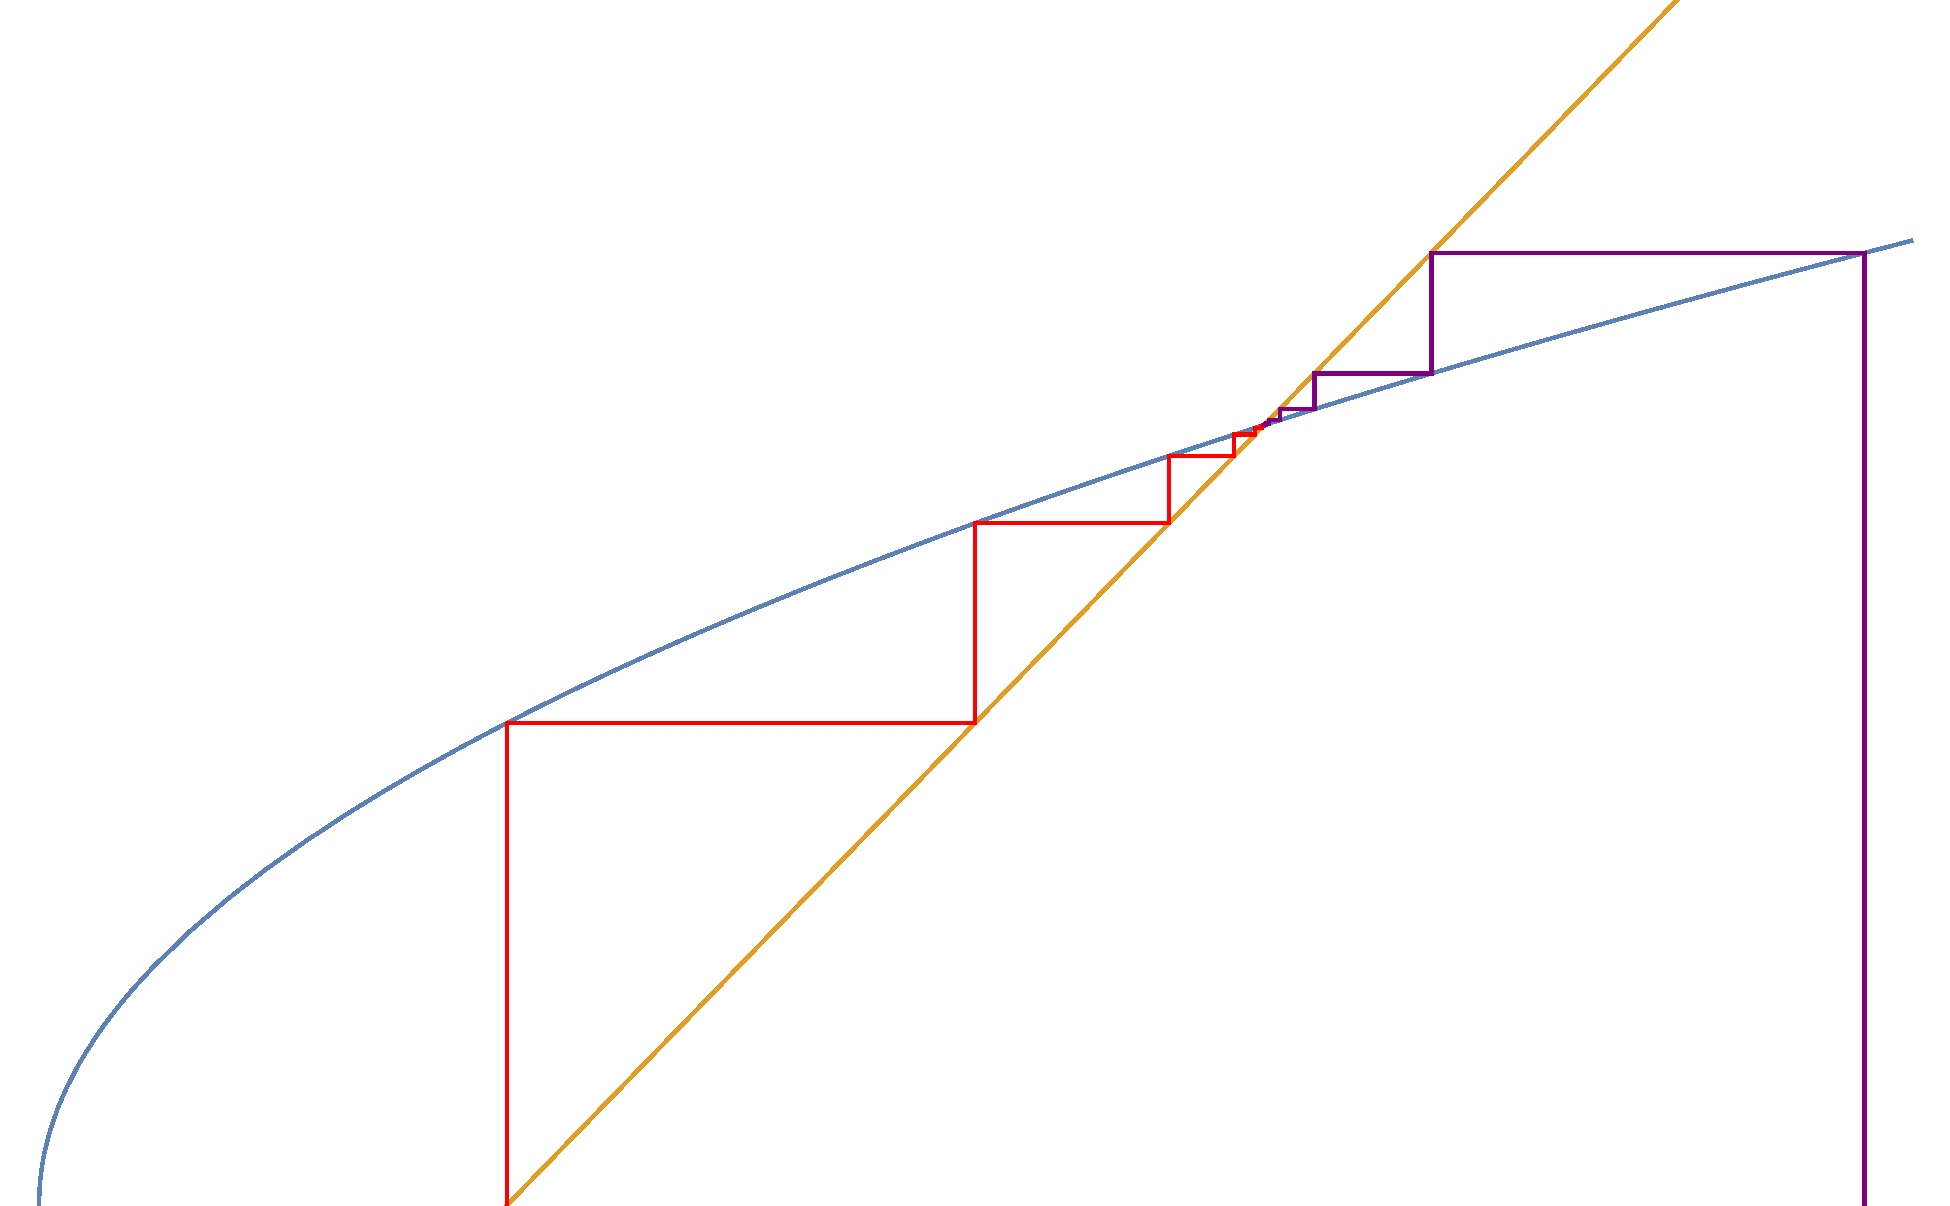
\includegraphics[scale=0.3]{../../Commun/Images/maths-cours-turtle-1.pdf}};
\draw[->] (-5,-3.06) -- (6,-3.06) node[below] {$x$};
\draw[->] (-2.38,-3.06) -- (-2.38,3.5) node[left] {$y$};
\node at (5.8,1.9) {$y=\sqrt{1+x}$};
\node at (4.15,3.05) {$y=x$};
\end{tikzpicture}
\end{center}
\begin{sol}
On commence par montrer que $(u_n)$ est bien définie en prouvant l'assertion $H_n$:"$u_n\geq 0$" par récurrence.

Recherche de points fixes : on tombe sur $(1+\sqrt{5})/2$.

On résout pour $x\geq 0$, $\sqrt{1+x}\geq x \Longleftrightarrow \ldots \Longleftrightarrow 0\leq x \leq (1+\sqrt{5})/2$.

\begin{itemize}
\item[$\bullet$] 1er cas : $\alpha> (1+\sqrt{5})/2$.

On démontre par récurrence $H_n : "(1+\sqrt{5})/2 \leq u_{n+1}\leq u_n".$
$(u_n)$ est donc décroissante minorée donc convergente et ça ne peut être que vers $(1+\sqrt{5})/2$.
\item[$\bullet$] 2ème cas : $\alpha < (1+\sqrt{5})/2$.
On démontre par récurrence $H_n : "(1+\sqrt{5})/2 \geq u_{n+1}\geq u_n".$
$(u_n)$ est donc croissante majorée donc convergente et ça ne peut être que vers $(1+\sqrt{5})/2$.
\end{itemize}
\end{sol}  
\exo Soit $\alpha\in\R$ et $(u_n)$ la suite définie par
  \[u_0\defeq\alpha \et \forall n\in\N \qsep u_{n+1}\defeq\frac{u_n^2+2}{3}.\]
 Étudier la limite éventuelle de la suite $(u_n)$.
% \begin{center}
% \begin{tikzpicture}[>=latex]
% \node at (0,0) {\includegraphics[scale=0.45]{../../Commun/Images/maths-cours-turtle-2.pdf}};
% \draw[->] (-7,-4.59) -- (5,-4.59) node[below] {$x$};
% \draw[->] (-5.435,-4.59) -- (-5.435,4.7) node[left] {$y$};
% \node at (1.8,4.6) {$y=\dfrac{x^2+2}{3}$};
% \node at (4.3,4.6) {$y=x$};
% \end{tikzpicture}
% \end{center}

\begin{sol}
$f$ est décroissante sur $\RM$ et croissante sur $\RP$.

On étudie les points fixes. On trouve $1$ et $2$.

On résout $f(x)\geq x$ : $S=[-\infty;1]\cup [2;+\infty]$.

\begin{itemize}
\item[$\bullet$] Si $\alpha \in [0;1]$. On souhaite montrer que $(u_n)$ est croissante et tend vers $1$. 
On commence par montrer par récurrence que $0\leq u_n\leq 1$. On en déduit que $(u_n)$ est croissante (de l'étude du signe de $f(x)-x$). Ainsi $(u_n)$ est croissante et majorée (par $1$) donc est convergente vers $\ell$. Puis un passage à la limite nous donne $\ell=\dfrac{\ell^2+2}{3}$ donc $\ell \in \set{1;2}$. Ainsi, $\ell=1$.


\item[$\bullet$] Si $\alpha \in [1;2[$, on montre successivement $1\leq u_n\leq 2$ par récurrence puis $u_{n+1}\leq u_n$. Ainsi $(u_n)$ est décroissante et minorée (par $1$) donc est convergente vers $\ell$. Puis un passage à la limite nous donne $\ell=\dfrac{\ell^2+2}{3}$ donc $\ell \in \set{1;2}$. Mais $u_n\leq u_0<0$ donc par passage à la limite, $\ell\leq u_0<0$  Ainsi, $\ell=1$.

\item[$\bullet$] Si $\alpha=2$, la suite est constante égale à $2$.

\item[$\bullet$] Si $\alpha \in ]2;+\infty[$. Par croissance de $f$ sur $]2;+\infty[$, on montre que $u_n>2 \forall n \in \N$. On montre ensuite que $u_{n+1}\geq u_n$. Ainsi, $u_n$ tend vers $\ell \in \R\cup\set{+\infty}$. Si $\ell$ est finie, un passage à la limite donne $\ell \in \set{1;2}$. Or $\forall n \in \N$, $2<u_0\leq u_n$ d'où $2<u_0\leq \ell$, ce qui est absurde. Donc $\ell=+\infty$.

\item[$\bullet$] Enfin si $\alpha \leq 0$, on remarque que $f(u_0)=f(|u_0|)$ par parité donc on est ramené au cas où $u_0\geq 0$. Ainsi,
\begin{itemize}
\item si $\alpha \in ]-2;2[$, $(u_n)$ tend vers $1$.
\item si $\alpha \in \set{-2;2}$, alors $(u_n)$ tend vers $2$.
\item si $\alpha \in ]-\infty;-2[\cup ]2;+\infty[$, alors $(u_n)$ tend vers $+\infty$.
\end{itemize}
\end{itemize}
\end{sol}
% \exo Soit $\alpha\in\R$ et $(u_n)$ la suite définie par $u_0\defeq\alpha$ et $\forall n\in\N \qsep u_{n+1}\defeq\cos(u_n)$. Étudier la convergence de la suite
%   $(u_n)$.
%   \begin{sol}
%   Montrer d'abord les lemmes suivants~: Si $I$ est stable par $f$ et que $f$
%   est croissante sur $I$, $(u_n)$ est monotone. Si $(u_{2n})$ et $(u_{2n+1})$
%   convergent vers la même limite alors $(u_n)$ est convergente. Les
%   points fixes de $f$ sont point fixe de $f\circ f$, mais la réciproque est
%   fausse.
%   Ensuite, on montrer que $\interf{0}{1}$ est stable par $\cos$ et que l'on
%   peut supposer que $\alpha\in\interf{0}{1}$. On montre que les suites
%   $(u_{2n})$ et $(u_{2n+1})$ sont monotones et donc convergent. Elles convergent
%   vers un point fixe de $cos\circ\cos$~: il n'y en a qu'un seul, le point fixe
%   de $\cos$.
%   \end{sol}
% \exo Soit $(u_n)$ la suite définie par
% \[u_0\defeq 1 \et \forall n\in\N\qsep u_{n+1}\defeq\frac{2u_n+2}{u_n+2}.\]
% \begin{questions}
% \question Montrer que la fonction $f$ définie sur $\RP$ par
%   \[\forall x\in\RP\qsep f(x)\defeq\frac{2x+2}{x+2}\]
%   admet un unique point fixe $\alpha$.
% \question Montrer que $f$ est contractante. En déduire que $u_n\tendvers{n}{+\infty}\alpha$.
% \end{questions}
\end{exos}

\begin{remarqueUnique}
\remarque Si $f$ est décroissante, on étudie les
      suites $(u_{2n})$ et $(u_{2n+1})$. Ces suites vérifient une relation de
      récurrence faisant intervenir $f\circ f$. On commence par étudier la suite $(u_{2n})$. Comme $f$ est décroissante, $f\circ f$ est croissante, et on est ramené au cas précédent. Puis, en remarquant que $u_{2n+1}=f(u_{2n})$, on en déduit la limite, si elle existe, de $(u_{2n+1})$. Si ces deux suites
      admettent la même limite $l\in\R$, alors $(u_n)$ converge vers $l$. Dans
      le cas contraire, la suite $(u_n)$ est divergente.
\end{remarqueUnique}


\begin{exoUnique}
\exo Étudier la suite $(u_n)$ définie par
\[u_0\defeq 0\et\forall n\in\N\qsep u_{n+1}\defeq 1-\frac{3}{4}u_n^2.\]
\begin{center}
\begin{tikzpicture}[>=latex]
\node at (0,0) {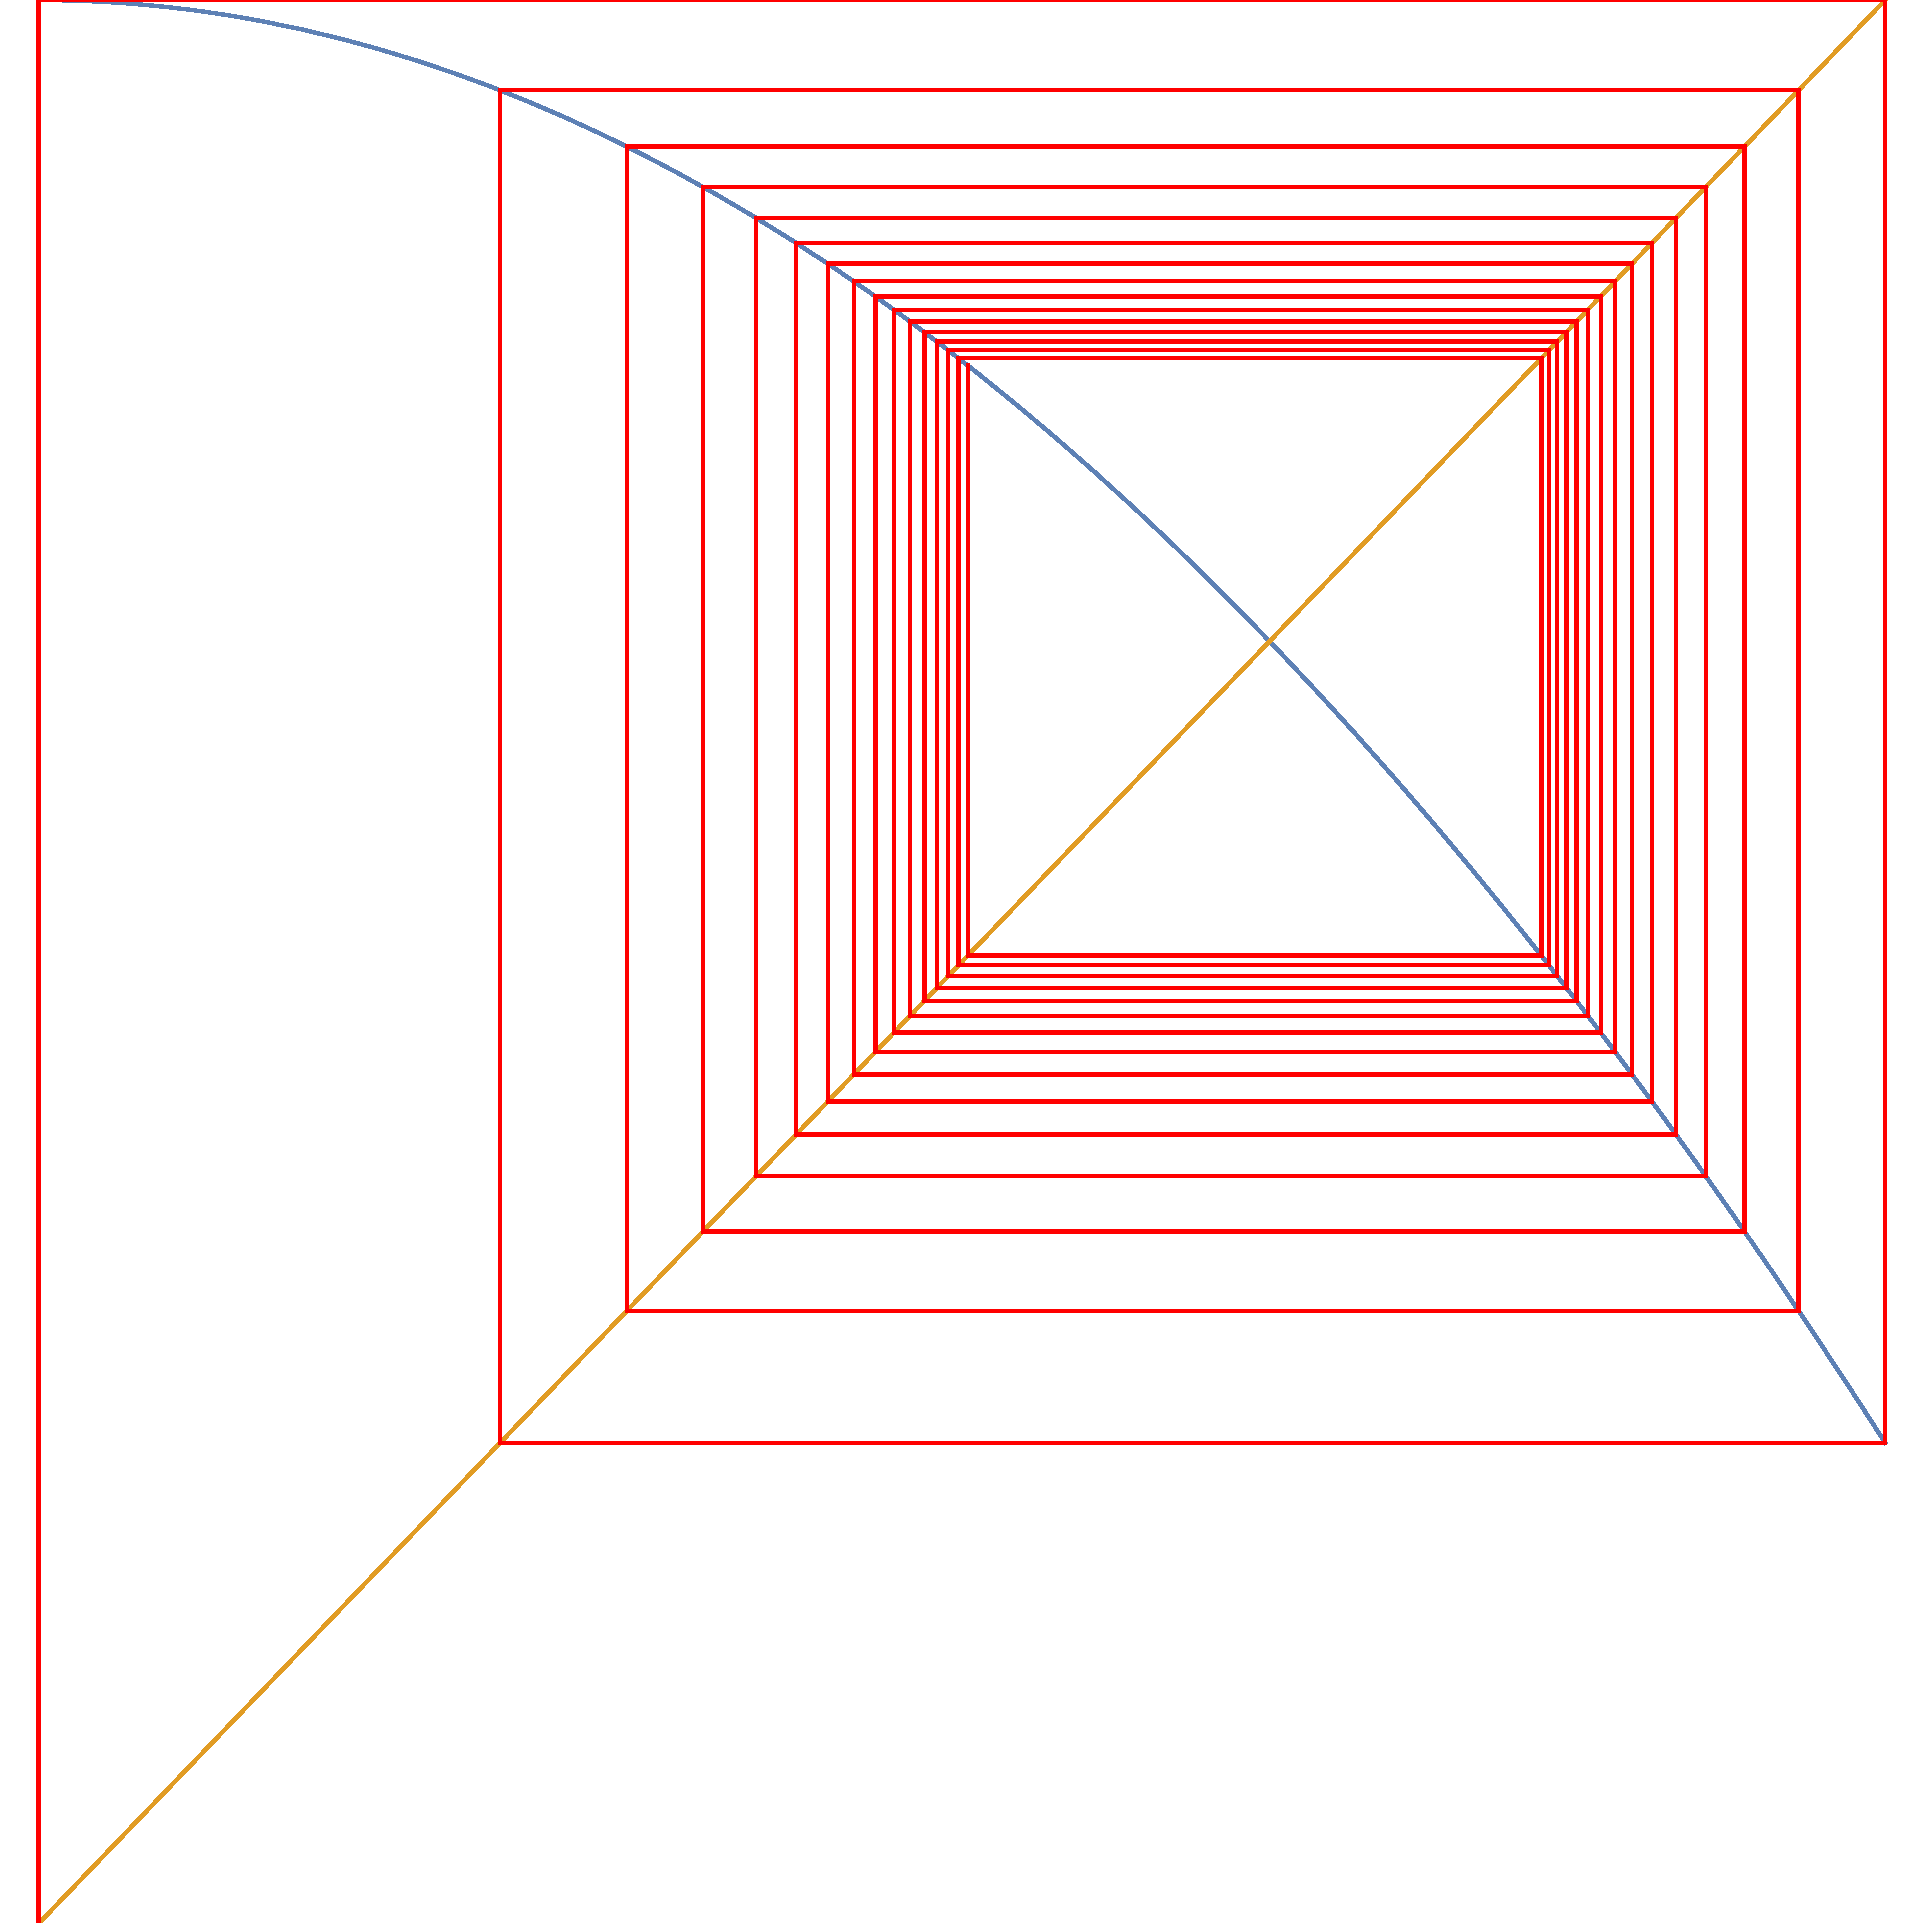
\includegraphics[scale=0.27]{../../Commun/Images/maths-cours-turtle-3.pdf}};
\draw[->] (-4.22,-4.4) -- (5.3,-4.4) node[below] {$x$};
\draw[->] (-4.22,-4.4) -- (-4.22,5.3) node[left] {$y$};
\node at (5.3,-2.15) {$y=1-\dfrac{3}{4}x^2$};
\node at (4.8,4.4) {$y=x$};
\end{tikzpicture}
\end{center}
\end{exoUnique}

\begin{sol}
Remarquons que 
\begin{itemize}
\item $f$ est décroissante sur $\RP$ et croissante sur $\RM$ donc $f\circ f$ est croissante.
\item Les points fixes de $f$ sont $-2$ et $2/3$.
\item ($f$ est paire.)
\end{itemize}
Nous allons donc étudier $(u_{2n})$ puis $(u_{2n+1})$.
\begin{itemize}
\item[$\bullet$] Déjà, $0\leq u_0\leq 2/3$ et si $0\leq u_{2n} \leq 2/3$ par croissance de $f\circ f$, on a $1/4=(f\circ f)(0)\leq (f\circ f)(u_{2n})=u_{2n+2} \leq (f\circ f)(2/3)=2/3$ donc par récurrence $0\leq u_{2n} \leq 2/3$ $\forall n \in \N$. 

De plus, $$(f\circ f)(x)-x=\frac{-1}{64}\p{27x^4-72x^2+64x-16}=\frac{-1}{64}(3x-2)(9x^3+6x^2-20x+8)$$ donc $$(f\circ f)(x)-x=\frac{-1}{64}(3x-2)(x+2)(9x^2-12x+4)=\frac{-1}{64}(3x-2)^3(x+2).$$
On peut alors dresser le tableau de signes de $(f\circ f)(x)-x$. Cela nous permet alors de dire que $(u_{2n})$ est croissante et majorée (par $2/3$) donc converge vers une limite $\ell$ qui par passage à la limite ne peut être que $2/3$.

\item[$\bullet$] $2/3\leq u_1 $ et par croissance de $f\circ f$, on déduit que $\forall n \in \N, 2/3\leq u_{2n+1}$. Avec le signe de $(f\circ f)(x)-x$ on peut voir que $(u_{2n+1})$ est décroissante et minorée (par $2/3$) donc converge vers une limite $\ell$ qui par passage à la limite ne peut être que $2/3$.

\end{itemize}

Pour conclure, $(u_{2n})$ et $(u_{2n+1})$ convergent vers une même limite donc $(u_n)$ est convergente (vers $2/3$).
\end{sol}

\subsection{Suites adjacentes}

\begin{definition}[utile=-3]
Soit $\p{u_n}$ et $\p{v_n}$ deux suites réelles. On dit que $\p{u_n}$ et
$\p{v_n}$ sont \emph{adjacentes} lorsque
\begin{itemize}
\item $\forall n\in\N \qsep u_n \leq v_n$,
\item $\p{u_n}$ est croissante et $\p{v_n}$ est décroissante,
\item $v_n-u_n \tendvers{n}{+\infty} 0$.
\end{itemize}
\end{definition}

\begin{remarqueUnique}
\remarque Si deux suites $(u_n)$ et $(v_n)$ vérifient les deux derniers points,
  alors elles vérifient le premier point. En théorie il est donc inutile de
  le vérifier, mais l'usage veut qu'on le fasse.
\end{remarqueUnique}

\begin{sol}
On va le montrer au travers de la prochaine preuve. On n'utilisera pas $(i)$ comme hypothèse, mais comme une conséquence de $(ii)$ et $(iii)$.
\end{sol}

\begin{proposition}[utile=-3]
Soit $\p{u_n}$ et $\p{v_n}$ deux suites adjacentes. Alors $\p{u_n}$ et $\p{v_n}$
convergent vers la même limite $l\in\R$. De plus
\[\forall n\in\N \qsep u_n \leq l \leq v_n.\]
\end{proposition}

\begin{preuve}
On suppose $u$ croissante et $v$ décroissante.
La suite $w=u-v$ est donc croissante et tend vers $0$. Donc $w_n\leq 0$. En effet, raisonnons par l'absurde. S'il existe un rang $N$ tel que $w_N>0$ par croissance, tous les rangs suivants sont $\geq w_N$ + passage à la limite.... Ainsi, $u_n\leq v_n\leq v_0$.
$u$ est croissante et majorée par $v_0$ donc converge vers $\ell$. $v=(v-u)+u$ converge donc vers $\ell$ aussi. 
\end{preuve}

\begin{exoUnique}
\exo Montrer que les suites $(u_n)$ et $(v_n)$ définies par
  \[\forall n\in\Ns \qsep u_n\defeq\sum_{k=1}^n \frac{1}{n+k} \et
    v_n\defeq\sum_{k=n}^{2n} \frac{1}{k}\]
  sont adjacentes. En utilisant une comparaison avec des intégrales, montrer
  qu'elles convergent vers $\ln 2$.
\end{exoUnique}

\begin{sol}
On a 
$$v_{n+1}-v_n=\frac{-3n-2}{n(2n+1)(2n+2)}\leq 0$$
donc $(v_n)$ est décroissante et $$u_{n+1}-u_n=\frac{1}{(2n+1)(2n+2)}\geq 0$$ donc $(u_n)$ est croissante. De plus, $v_n-u_n=\dfrac{1}{n}$.
Donc les suites sont adjacentes et convergent vers la même limite $\ell$.
En outre, $\forall k\geq 2$, $$\ln(k+1)-\ln(k)=\integ{k}{k+1}{\frac{1}{x}}{x}\leq \frac{1}{k} \leq \integ{k-1}{k}{\frac{1}{x}}{x}=\ln(k)-\ln(k-1)$$ donc $\forall n\geq 2$, on a en sommant de $n$ à $2n$ :
$$\ln(2n+1)-\ln(n)\leq v_n \leq \ln(2n)-\ln(n-1).$$
\end{sol}

\subsection{Théorème de \nom{Bolzano-Weierstrass}}

\begin{theoreme}[nom={Théorème de \nom{Bolzano-Weierstrass}}]
Toute suite bornée admet une sous-suite convergente.
\end{theoreme}

\begin{preuve}
\begin{itemize}
\item[$\bullet$] \underline{Cas réel (par dichotomie) :} Soit $u$ une suite réelle bornée. On peut fixer $K>0$ tel que $\forall n\in \N, u_n\in \interf{-K}{K}$. Posons $a_0=-K$, $b_0=K$ et $\varphi(0)=0$. On a bien $u_{\varphi(0)}\in \interf{a_0}{b_0}$.\\
Définissons \[E_0=\ens{n\in\N | u_n \in \interf{-K}{0}} \text{ et } E'_0=\ens{n\in\N | u_n \in \interf{0}{K}}.\] L'une au moins des deux parties est infinie, on choisit l'intervalle correspondant et on note $[a_1,b_1]$ cet intervalle. Comme l'ensemble choisi est infini, on peut en particulier fixer un élément $u_{\varphi(1)}$ dans $[a_1,b_1]$ tel que $\varphi(1)>\varphi(0)$.\\
Soit $p\in \N$. Supposons construit $\interf{a_p}{b_p} \subset\interf{a_{p-1}}{b_{p-1}}\subset\ldots\subset\interf{a_0}{b_0}$ et $\varphi(0)<\varphi(1)<\ldots<\varphi(p)$. Définissons \[E_p=\ens{n\in\N | u_n \in \interf{a_p}{\frac{a_p+b_p}{2}}} \text{ et } E'_p=\ens{n\in\N | u_n \in \interf{\frac{a_p+b_p}{2}}{b_p}}.\]
L'union des deux est infinie par construction donc l'un des deux est infini. On le choisit et on note $\interf{a_{p+1}}{b_{p+1}}$ l'intervalle correspondant. Comme l'ensemble choisi est infini, on peut en particulier fixer un élément $u_{\varphi(p+1)}$ dans $\interf{a_{p+1}}{b_{p+1}}$ tel que $\varphi(p+1)>\varphi(p)$.\\

On construit ainsi, par récurrence, une suite de segments de $\R$ décroissante au sens de l'inclusion et telle que $b_n-a_n=\dfrac{2K}{2^n}$ et telle que $\forall n\in \N$, $u_{\varphi(n)}\in \interf{a_n}{b_n}$.

D'après le théorème des segments emboités, $\displaystyle \bigcap_{n\in \N}\interf{a_n}{b_n}=\ens{\ell}$.

$\forall n\in \N$, comme $u_{\varphi(n)}$ et $\ell$ sont dans $\interf{a_n}{b_n}$, on a : $\abs{u_{\varphi(n)}-\ell}\leq \dfrac{2K}{2^n}$ d'où le résultat d'après le théorème des gendarmes.
\item[$\bullet$] \underline{Cas complexe :} Soit $u\in\C^\N$ bornée. Posons $x=\Re u$ et $y=\Im u$. Comme $u$ est bornée, $x$ l'est. D'après le cas réel, il existe une extraction $\varphi_1$ et un réel $\alpha$ tels que $x_{\varphi_1(n)}\tendvers{n}{+\infty}\alpha$.

La suite $(y_{\varphi_1(n)})_{n\in\N}$ est bornée. Il existe donc une extraction $\varphi_2$ et un réel $\beta$ tels que $y\circ \varphi_1 \circ \varphi_2=(y_{\varphi_1\circ\varphi_2(n)})_{n\in\N}$ converge vers $\beta$.
Posons $\varphi=\varphi_1\circ\varphi_2$. C'est une extraction. $x\circ\varphi$ est convergente comme suite extraite de $x\circ\varphi_1$ et $y\circ\varphi$ aussi.\\

Finalement, $u\circ \varphi$ est convergente.
\end{itemize}
\end{preuve}

\begin{exoUnique}
\exo Soit $x\in\R\setminus\Q$, $(p_n)$ une suite d'entiers relatifs et
  $(q_n)$ une suite d'entiers naturels non nuls tels que
  \[\frac{p_n}{q_n}\tendvers{n}{+\infty} x.\]
  Montrer que $q_n\tendvers{n}{+\infty}+\infty$.
\end{exoUnique}
\begin{sol}
Raisonnons par l'absurde. Cela signifie qu'il existe $m\in \R$ tel que $\forall N \in \N, \exists n\geq N$ tel que $q_n < m$.
Fixons un tel $m$ et construisons une extractrice $\phi$ telle que $\forall n \in \N$, $1\leq q_{\phi(n)}\leq m$.
\begin{itemize}
\item[$\bullet$] On pose $N=0$. Il existe $n\geq 0$ tel que $q_n<m$. On pose $n=\phi(0)$.
\item[$\bullet$] Soit $k\in \N$. On suppose construit $\phi(0)< \ldots< \phi(k)$ tels que $1\leq u_{\phi(k)}\leq m$.
On pose $N=\phi(k)+1$. Alors, il existe $n\geq N$ tel que $q_n<m$. On pose $\phi(k+1)=n$...
\end{itemize}
La suite $(q_{\phi(n)})$ est donc bien construite et bornée. Elle admet donc une sous-suite convergente, c'est-à-dire qu'il existe $\psi$ telle que $(q_{\phi(\psi(n))})$ converge vers $\ell \in \R$. Comme il s'agit d'une suite d'entiers convergentes, elle est constante apcr et donc $\ell \in \Ns$. Mais alors $\displaystyle p_{\phi(\psi(n))}=\frac{p_{\phi(\psi(n))}}{q_{\phi(\psi(n))}}q_{\phi(\psi(n))} \tendvers{n}{+\infty}{\ell x}=\ell'$ et pour les mêmes raisons $\ell' \in \Z$.
Ainsi, $\displaystyle \frac{p_{\phi(\psi(n))}}{q_{\phi(\psi(n))}} \tendvers{n}{+\infty} \frac{\ell'}{\ell} \in \Q$. Donc $x\in \Q$ par unicité de la limite, ce qui fournit une contradiction.
\end{sol}
%END_BOOK

\end{document}



\section{Exercices}
\setcounter{numeroexercice}{1}
\documentclass{magnolia}

\magtex{tex_driver={pdftex}}
\magfiche{document_nom={Exercices sur les suites},
          auteur_nom={François Fayard},
          auteur_mail={fayard.prof@gmail.com}}
\magexos{exos_matiere={maths},
         exos_niveau={mpsi},
         exos_chapitre_numero={8},
         exos_theme={Suites}}
\magmisenpage{}
\maglieudiff{}
\magprocess

\begin{document}

%BEGIN_BOOK

\magsection{Suite réelle et complexe}
\magsubsection{Définition}
\magsubsection{Suite et relation d'ordre}


\magsection{Notion de limite}
\magsubsection{Limite finie}


\exercice{nom={Minimum et Maximum}}
Soit $u$ et $v$ deux suites réelles convergeant respectivement vers $l_u$ et
$l_v$. Montrer que les suites de terme général $\max(u_n,v_n)$ et
$\min(u_n,v_n)$ sont convergentes et calculer leurs limites.
\begin{sol}
On utilise les expressions du max et du min avec les valeurs absolues et on passe à la limite !
\end{sol}

\exercice{nom={Plus grand et plus petit élément}}
Soit $(u_n)$ une suite de réels. On pose
\[A\defeq\ensim{u_n}{n\in\N}.\]
\begin{questions}
\question On suppose que $(u_n)$ diverge vers $+\infty$. Montrer que $A$ admet un plus petit
  élément.
\question On suppose que $(u_n)$ converge. Montrer que $A$ admet un plus petit ou un plus grand  élément.
\end{questions}

\exercice{nom={Quelques calculs de limite}}
Montrer que les suites suivantes, définies par leur terme général, admettent une
limite que l'on calculera.
\[\textbf{a.}\ \frac{\sin (n^3)}{n}, \qquad \textbf{b.}\ \frac{n^3+5n}{5n^3+\cos n+\frac{1}{n^2}}, \qquad
\textbf{c.}\ \frac{2n+(-1)^n}{5n+(-1)^{n+1}}, \qquad \textbf{d.}\ \sqrt[n]{3+\sin n},\]
\[\textbf{e.}\ \p{1-\frac{1}{\sqrt{n}}}^n,\qquad \textbf{f.}\ \arctan\left(\frac{n^2-n\cos n +(-1)^n}{\ln n + n^2}\right), \qquad
\textbf{g.}\ \left(5\sin\frac{1}{n^2}+\frac{1}{5}\cos n\right)^n,\]
\[\textbf{h.}\ \frac{1}{n^2} \sum_{k=1}^{n} \ent{kx},
  \qquad \textbf{i.}\ \left(a+\frac{b}{n}\right)^n \quad
  \text{o\`u $a$ et $b$ sont réels et $a\geq 0$}.\]
\begin{sol}
\begin{questions}
\question $0$
\question $1/5$
\question $2/5$
\question mise sous forme exponentielle puis l'exposant tend vers $0$ donc ça tend vers $1$.
\question tend vers $\pi/4$ par composition de limites.
\question Il existe $N\in \N$ tel que $\forall n\geq N$, $\abs{5\sin\frac{1}{n^2}+\frac{1}{5}\cos n}\leq \dfrac{2}{5}$ d'où $\abs{5\sin\frac{1}{n^2}+\frac{1}{5}\cos n}^n\leq \p{\dfrac{2}{5}}^n$.
\question $$\frac{n+1}{2n}x-\frac{1}{n}\leq \frac{1}{n^2} \sum_{k=1}^{n} (kx-1)<\frac{1}{n^2} \sum_{k=1}^{n} \ent{kx}\leq \frac{1}{n^2} \sum_{k=1}^{n} kx=\frac{n+1}{2n}x.$$
\question Si $a=0$, $\displaystyle\abs{\frac{b}{n}}\leq \p{\frac{1}{2}}^n$ apcr, d'où la limite vaut $0$. Sinon, $$\left(a+\frac{b}{n}\right)^n=a^n\underbrace{\p{1+\frac{b}{an}}^n}_{\tendvers{n}{+\infty}{\e^{b/a}}}$$ donc selon $a$, ...
\end{questions}
\end{sol}

\exercice{nom={Une manipulation fine d'$\epsilon$}}
Soit $(u_n)$ une suite réelle telle que
\[\forall k,n \geq 1 \qsep 0\leq u_n \leq  \frac{k}{n}+\frac{1}{k}.\]
Le but de cet exercice est de montrer que $(u_n)$ converge vers $0$ de deux
manières distinctes.
\begin{questions}
\question
  \begin{questions}
  \question Soit $\epsilon > 0$. Montrer qu'il existe une constante $C$
    telle que
    $$\forall n \geq 1 \qsep |u_n|\leq \frac{C}{n} + \frac{\epsilon}{2}.$$
  \question En déduire que $(u_n)$ converge vers $0$.
  \end{questions}
\question Montrer directement ce résultat en choisissant judicieusement $k$.
\end{questions}
\begin{sol}
Dernière question, il suffit de prendre $k=\ent{\sqrt{n}}$.
\end{sol}

\exercice{nom={Théorème de \nom{Césaro}}}
Étant donnée une suite complexe $(u_n)$, on définit la suite $(c_n)$ par
\[\forall n \geq 1 \qsep c_n\defeq\frac{u_1+u_2+\dots+u_n}{n}=\frac{1}{n}
  \sum_{k=1}^{n} u_k\]
appelée moyenne de \nom{Césaro} de la suite $(u_n)$. 
\begin{questions}
\question On suppose dans cette question que $(u_n)$ est convergente. Il existe donc
  $l\in\C$ tel que
  \[u_n\tendvers{n}{+\infty}l.\]
  On souhaite montrer que $(c_n)$ converge vers $l$.
  \begin{questions}
  \question Soit $\epsilon>0$. Montrer qu'il existe $N_0\in\Ns$ tel que
    \[\forall n \geq N_0 \qsep \abs{c_n-l}\leq \frac{\abs{u_1-l}+\dots+\abs{u_{N_0-1}-l}}{n} +
      \frac{\epsilon}{2}.\]
  \question En déduire qu'il existe $N\in\Ns$ tel que
    \[\forall n \geq N \qsep |c_n-l|\leq \epsilon\]
    et conclure.
  \end{questions}
\question Réciproquement, on suppose $(c_n)$ convergente. Peut-on en déduire que
  $(u_n)$ est convergente~?
\question Que dire si $(u_n)$ est une suite réelle divergeant vers $+\infty$~?
\end{questions}
\begin{sol}
Pour la dernière question, cela fonctionne aussi, il suffit de fixer $M>0$ puis $N$ à partir duquel $u_n\geq 2M$. Alors $\forall n\geq N$, on sépare les sommes et on se retrouve avec $$S_n \geq \frac{\sum_{k=0}^{N-1}u_k-2MN}{n+1}+2M$$ le premier terme tendant vers $0$, il est en particulier $\geq -M$ apcr $N_1$. Il reste à prendre $n\geq \max(N,N_1)$.
\end{sol}


\exercice{nom={Applications du théorème de \nom{Césaro}}}
Dans cet exercice, on pourra utiliser librement le théorème de \nom{Césaro}.
\begin{questions}
\question Soit $(u_n)$ une suite complexe telle que $u_{n+1}-u_n$ converge vers
    $l\in\C$. Montrer que
    \[\frac{u_n}{n} \tendvers{n}{+\infty} l.\]
\question Soit $(u_n)$ une suite de réels strictement positifs convergeant vers
    un réel $l>0$. Montrer que
    \[\sqrt[n]{\prod_{k=1}^{n} u_k}  \tendvers{n}{+\infty} l.\]
\end{questions}

\exercice{nom={Autour de \nom{Césaro}}}

Soit $(u_n)$ une suite complexe convergeant vers $l\in\C$. 
\begin{questions}
\question Montrer que la suite $(v_n)$ définie par
  \[\forall n\in\Ns \qsep v_n\defeq\frac{u_1+2u_2+\dots+nu_n}{n^2}=
    \frac{1}{n^2} \sum_{k=1}^{n} k u_k\]
  converge vers $l/2$.
\question Montrer que la suite $(w_n)$ définie par 
  \[\forall n\in\N \qsep w_n\defeq\frac{\binom{n}{0}u_0+ \binom{n}{1}u_1+
    \dots+\binom{n}{n}u_n}{2^n}=\frac{1}{2^n} \sum_{k=0}^{n}
    \binom{n}{k} u_k\]
  converge vers $l$.
% \question Soit $u$ et $v$ deux suites complexes. On définit la suite
%   $P(u,v)$ définie par~:
%   $$\forall n \geq 1 \quad P(u,v)_n=\frac{u_1 v_n+u_2 v_{n-1}+
%     \dots+u_n v_1}{n}$$
%   \begin{questions}
%   \question Montrer que si $u$ converge vers $0$ et $v$ est bornée, alors
%     $P(u,v)$  converge vers~$0$.
%   \question En déduire que si $u$ et $v$ convergent respectivement vers
%     $l_u$ et $l_v$, alors $P(u,v)$ converge vers $l_u l_v$.
%   \end{questions}
\end{questions}


\exercice{nom={Produit de \nom{Cauchy}}}
Soit $(u_n)$ et $(v_n)$ deux suites complexes convergeant vers 0. On suppose qu'il existe
$M\in\RP$ tel que
\[\forall n\in\N\qsep \sum_{k=0}^n \abs{u_k}\leq M.\]
Montrer que
\[\sum_{k=0}^n u_k v_{n-k} \tendvers{n}{+\infty}0.\]


\magsubsection{Limite infinie}
\magsubsection{Limite et relation d'ordre}

\exercice{nom={Calcul de limite}}
\begin{questions}
\question Montrer que
   \[\forall p\in\Ns \quad
     \frac{1}{p+1} \leq \ln\p{\frac{p+1}{p}} \leq \frac{1}{p}.\]
\question En déduire la limite de la suite de terme général
   \[\sum_{k=1}^n \frac{1}{n+k}.\]
\end{questions}
\begin{sol}
\begin{questions}
\question
\begin{eqnarray*}\ln\p{1+\frac{1}{x}}-\frac{1}{1+x}\geq 0 &\Longleftrightarrow & \ln\p{\frac{x+1}{x}}\geq\frac{1}{1+x}\\
&\Longleftrightarrow & -\ln\p{\frac{x}{x+1}}\geq\frac{1}{1+x}\\
&\Longleftrightarrow & \ln\p{1-\frac{1}{x+1}}\leq-\frac{1}{x+1} \text{ ce qui est vrai.}
\end{eqnarray*}
\question On en déduit
   \[\sum_{k=1}^n\ln\p{\frac{n+k+1}{n+k}} \leq \sum_{k=1}^n \frac{1}{n+k}\leq \sum_{k=1}^n\ln\p{\frac{n+k}{n+k-1}}.\]
   Puis somme télescopique et théorème des gendarmes.
\end{questions}
\end{sol}

\exercice{nom={Exercice}}
Soit $(u_n)$ et $(v_n)$ deux suites d'éléments de $[0,1]$ telles que
\[u_n v_n\tendvers{n}{+\infty} 1.\]
Montrer que $(u_n)$ et $(v_n)$ convergent toutes les deux vers 1.



\magsubsection{Théorèmes usuels et limites usuelles}
\magsubsection{Suite extraite}







% \magsection{Définition de la convergence}

% \exercice{nom={Manipulation d'$\epsilon$}}
% \begin{questions}
% \question Montrer qu'une suite complexe $u$ converge vers $l$ si et seulement
%   si~:
%   $$\forall \epsilon > 0 \quad \exists N \in \N \quad \forall n
%     \geq N \quad |u_n-l|< \epsilon$$
% \question Que dire d'une suite $u$ telle que~:
%   $$\exists N \in \N \quad \forall \epsilon > 0 \quad \forall n
%   \geq N \quad |u_n-l|\leq \epsilon$$
% \question Montrer que toute suite convergente à valeurs entières est constante
%   à partir d'un certain rang.
% \question Soit $u$ une suite réelle telle que $u_{n+1}-u_n$ converge vers
%   $l>0$. Montrer que $u$ diverge vers $+\infty$.
% \question Montrer que si deux suites réelles $u$ et $v$ respectivement
%   majorées par $a$ et $b$ sont telles que $u+v$ converge vers $a+b$, alors $u$
%   converge vers $a$ et $v$ converge vers $b$.
% \question Montrer qu'une suite complexe $u$ converge vers $l$ si et seulement
%   si quelque soit $\epsilon > 0$, l'ensemble
%   $A_{\epsilon}=\{n \in \N : |u_n-l|\geq \epsilon\}$ est fini.
%   En déduire que si $u$ converge vers $l$ et si $\phi$ est une bijection de
%   $\N$, alors la suite de terme général $u_{\phi(n)}$ converge vers
%   $l$ (La notion de limite ne dépend pas de l'ordre de la suite).
% \end{questions}

% \magsection{Suites extraites}

\exercice{nom={Suites divergentes}}
Montrer que les suites suivantes, définies par leur terme général, sont
divergentes
\[\textbf{a.}\ \cos\p{\frac{n\pi}{4}}, \qquad \textbf{b.}\ \frac{5n^2+\sin n}{2(n+1)^2 \cos\frac{n\pi}{5}},
  \qquad
  \textbf{c.}\ \frac{2+n\sin\p{\frac{n\pi}{2}}}{n\cos\p{\frac{\pi}{4}+\frac{n\pi}{2}}}.\]
  
  \begin{sol}
  \begin{questions}
  \question $u_{8n}=1$ et $u_{8n+4}=-1$.
  \question $v_{10n}\tendvers{n}{+\infty}2,5$ et $v_{10n+5}\tendvers{n}{+\infty}-2,5$
  \question $w_{4n}\tendvers{n}{+\infty}0$ et $w_{4n+1}\tendvers{n}{+\infty}-\sqrt{2}$
  \end{questions}
  \end{sol}


\exercice{nom={Autour de la notion d'extractrice}}
  \begin{questions}
  \question Soit $(u_n)$ une suite réelle prenant un nombre fini de valeurs.
    Montrer que l'on peut en extraire une suite constante.
  \question Soit $(u_n)$ une suite réelle ne divergeant pas vers $+\infty$.
    Montrer que l'on peut en extraire une suite majorée.
  \question Soit $(u_n)$ une suite complexe et $l\in \mathbb{C}$. Montrer
    l'équivalence entre les deux propositions suivantes.
  \begin{itemize}
  \item Il existe une suite extraite de $(u_n)$ convergeant vers $l$.
  \item Quel que soit $\epsilon > 0$, l'ensemble
    \[A_\epsilon=\enstq{n \in \N}{|u_n-l|\leq \epsilon}\]
    est infini.
  \end{itemize}
  Donner une exemple d'une suite non convergente vérifiant cette propriété.
\question Montrer que de toute suite réelle divergeant vers $+\infty$, on peut
  extraire une suite croissante.
\end{questions}

\exercice{nom={Convergence et suites extraites}}
\begin{questions}
\question Soit $(u_n)$ une suite réelle croissante. On suppose que $(u_n)$ admet une
  suite extraite convergente. Montrer que $(u_n)$ converge.
\question Montrer que si les suites extraites de terme général $u_{3n}$,
  $u_{3n+1}$ et $u_{3n+2}$ convergent vers le même complexe $l$, alors $(u_n)$
  converge vers $l$.
\question On suppose qu'il existe un réel $l$ tel que pour tout entier
  $k\geq 2$, la suite $(u_{kn})_{n\in\N}$ converge vers $l$.
  Peut-on en déduire la convergence de la suite $(u_n)$~?
\end{questions}



% \exercice{nom={Valeurs d'adhérence}}
% Soit $\p{u_n}$ une suite à valeurs dans $\C$. On dit que $z_0\in\C$ est une
% valeur d'adhérence de la suite $\p{u_n}$ lorsqu'il existe une extractrice
% $\phi$ telle que
% \[u_{\phi(n)}\tendvers{n}{+\infty} z_0.\]
% \begin{questions}
% \question Donner les valeurs d'adhérence des suites de terme général
%   \[\p{-1}^n, \qquad \frac{1}{n}+\sin\p{\frac{\ent{\sqrt{n}}\pi}{3}}.\]
% \question Montrer que $l\in\C$ est valeur d'adhérence de la suite $\p{u_n}$ si
%   et seulement si quelque soit $\epsilon>0$, l'ensemble
%   \[\enstq{n\in\N}{\abs{u_n-l}\leq\epsilon}\]
%   est infini.
% \question L'objet de cette question est de montrer que si une suite bornée
%   $\p{u_n}$ admet une et une seule valeur d'adhérence $l$, alors elle converge
%   vers $l$. On raisonne par l'absurde et on suppose que $\p{u_n}$ ne converge
%   pas vers $l$.
%   \begin{questions}
%   \question Montrer qu'il existe $\epsilon>0$ tel que l'ensemble
%     \[\enstq{n\in\N}{\abs{u_n-l}\geq\epsilon}\]
%     est infini.
%   \question En déduire qu'il existe une extractrice $\phi$ telle que
%     \[\forall n\in\N \qsep \abs{u_{\phi(n)}-l}\geq\epsilon.\]
%   \question Conclure.
%   \end{questions}
% \end{questions}

\magsection{Propriétés de $\R$}

\magsubsection{Voisinage}

\magsubsection{Densité}

\magsubsection{Propriété de la borne supérieure}



\exercice{nom={Comparaison de deux ensembles}}
Soit $A$ et $B$ deux parties non vides de $\R$ telles que 
\[\forall\p{a,b}\in A\times B \quad a\leq b\]
\begin{questions}
\question Montrer que $\sup(A)$ et $\inf(B)$ existent et que
  $\sup(A)\leq \inf(B)$. 
\question Si l'on suppose maintenant que quel que soit $\p{a,b}\in A\times B$ on
  a $a< b$, peut-on en conclure que $\sup(A)<\inf(B)$~?
\end{questions}

\begin{sol}
\begin{questions}
\question Fixons $b\in B$. D'après l'hypothèse,  $\forall a \in A, a\leq b$  donc est un majorant de $A$ qui est non vide donc $\sup A$ existe et on a $\sup A \leq b$. Et ceci est valable pour $b$ quelconque dans $B$. Ainsi, $B$ est minorée par $\sup A$ donc $\inf B$ existe et on a $\sup A \leq \inf B$.
\question NON. Prendre par exemple $A=\RMs$ et $B=\RPs$.
\end{questions}
\end{sol}


\exercice{nom={Borne supérieure}}
Soit $A$ une partie bornée non vide de~$\R$. Montrer que 
\[\sup_{\p{x,y}\in A^2}\abs{x-y}=\sup(A)-\inf(A).\]

\begin{sol}
Posons $B=\{|y-x|,\;(x,y)\in A^2\}$.
$A$ est une partie non vide et bornée de $\R$, et donc $m=\inf A$ et $M=\sup A$ existent dans $\R$.
Pour $(x,y)\in A^2$, on a $m\leq x\leq M$ et $m\leq y M$, et donc $y-x\leq M-m$ et $x-y\leq M-m$ ou encore $|y-x|\leq M-m$.
Par suite, $B$ est une partie non vide et majorée de $\R$. $B$ admet donc une borne supérieure.
Soit $\varepsilon>0$. Il existe $(x_0,y_0)\in A^2$ tel que $x_0<\inf A+\frac{\varepsilon}{2}$ et $y_0>\sup A-\frac{\varepsilon}{2}$.

Ces deux éléments $x_0$ et $y_0$ vérifient, 

$$|y_0-x_0|\geq y_0-x_0>\left(\sup A-\frac{\varepsilon}{2}\right)-\left(\inf A+\frac{\varepsilon}{2}\right)=\sup A-\inf A-\varepsilon.$$
En résumé, 
\begin{enumerate}
 \item  $\forall(x,y)\in A^2,\;|y-x|\leq\sup A-\inf A$ et  
 \item  $\forall\varepsilon>0,\;\exists(x,y)\in A^2/\;|y-x|>\sup A-\inf A-\varepsilon$.
\end{enumerate}
Donc, $\sup B=\sup A-\inf A$.

\end{sol}

% \exercice{nom={Borne supérieure non atteinte},
%           exercice_present={non}}
% Soit $A$ une partie non vide majorée de $\R$. On note~$a$ sa borne supérieure.
% On suppose que $a\not\in A$.
% \begin{questions}
% \question Montrer que pour tout $\epsilon>0$, il existe une infinité 
%   d'éléments de $A$ dans $\interof{a-\epsilon}{a}$.
% \question Montrer que pour tout $\epsilon>0$, il existe $x$ et $y$ distincts
%   dans $A$ tels dont la distance est plus petite que $\epsilon$.
% \end{questions}

\exercice{nom={Calcul de bornes supérieures}}
%On se place dans l'ensemble totalement ordonné $\p{\R,\leq}$.
Déterminer, si
elles ou ils existent, les bornes supérieures, bornes inférieures, plus grands
éléments, plus petits éléments des parties de $\R$ suivantes.
\begin{eqnarray*}
A&\defeq&\ensim{\frac{1}{n}+\frac{1}{p}}{\p{n,p}\in\Ns^2},\\
B&\defeq&\ensim{\frac{n-\frac{1}{n}}{n+\frac{1}{n}}}{n\in\Ns},\\
C&\defeq&\ensim{\frac{1}{n}+(-1)^p}{\p{n,p}\in\Ns\times\N}.
\end{eqnarray*}

\begin{sol}
$$\max(A)=2 \text{ et } \inf(A)=0.$$
$$\min(B)=0 \text{ et } \sup(B)=1.$$
$$\inf(C)=-1 \text{ et } \max(C)=2.$$

\end{sol}

% \exercice{nom={Borne supérieure},
%           exercice_present={non}}
% Soit~:
% \[A=\enstq{\p{\frac{m+n+1}{m+n}}^{m+n}}{\p{m,n}\in\Ns^2}\]
% Montrer que $A$ est majorée non vide. calculer $\sup(A)$.

\exercice{nom={Bornes supérieures}}
Soit $A$ et $B$ deux parties de $\R$ non vides et majorées. Soit $\lambda$
un nombre réel. On pose
\begin{eqnarray*}
C&\defeq&\ensim{a+b}{a\in A \quad b\in B},\\
D&\defeq&\ensim{\lambda\cdot a}{a\in A},\\
E&\defeq&\ensim{a\cdot b}{a\in A \quad b\in B}.
\end{eqnarray*}
\begin{questions}
\question Montrer que $\sup(C)$ existe et vaut $\sup(A)+\sup(B)$. 
\question Que peut-on dire de l'existence et de la valeur de $\sup(D)$,
  $\sup(E)$~? On pourra formuler des hypothèses supplémentaires adéquates sur $A$
  et $B$.
\end{questions}

\begin{sol}
\begin{questions}
\question$\sup A+\sup B$ majore $A+B$ donc $\sup(A+B)\leq \sup A+\sup B$.
Fixons $a\in A$. On a $\forall b\in B$ :
$$b\leq \sup(A+B)-a$$ donc $$\sup B \leq \sup(A+B)-a$$ et ce peu importe $a\in A$. Ainsi, $\sup(A+B)-\sup B$ majore $A$ d'où $\sup A\leq \sup(A+B)-\sup B$.
\question 
\end{questions}
\end{sol}

\exercice{nom={Un théorème de point fixe}}
Soit $I=[a,b]$ avec $a<b$ et soit $f:I\rightarrow I$ une application
croissante. Montrer qu'il existe $c\in I$ tel que $f(c)=c$. Considérer pour
cela la partie 
$$A=\enstq{x\in I}{f(x)>x}.$$ 
Quelle est l'interprétation géométrique de cette propriété en termes du graphe
de~$f$ ?

\begin{sol}
\begin{itemize}
\item[$\bullet$] Si $A=\emptyset$, cela signifie que $\forall x \in I, f(x)\leq x$. Or $f(a)\geq a$ (car $f(a)\in I$) donc $f(a)=a$.
\item[$\bullet$] Si $A\neq \emptyset$, $A$ étant majorée par $b$ admet un sup. $\sup(A)\in I$ car il est plus petit que $b$ et plus grand qu'un élément de $I$ ($A\neq \emptyset$). Posons $t=\sup A$.

$\forall x\in A$, $x\leq t$ donc par croissance de $f$ et puisque $x\in A$, $x<f(x)\leq f(t)$ donc $f(t)$ est un majorant de $A$. Ainsi, $f(t)\geq t$.
\begin{itemize}
\item Si $f(t)=t$, on a bien le résultat escompté.
\item Sinon, $f(t)>t=\sup A$ donc $f(t)\notin A$, c'est-dire que $f(f(t))\leq f(t)$ mais par croissance de $f$, $f(t)\leq f(f(t))$ donc $f(f(t))=f(t)$.
\end{itemize}
\end{itemize}
\end{sol}

\exercice{nom={Intervalle}}
Soit $I$ et $J$ deux intervalles de $\R$. Montrer que
\[I+J\defeq\ensim{x+y}{x\in I \et y\in J}\]
est un intervalle.

\begin{sol}
Soit $a,b \in I+J$. Soit $t\in [0,1]$. On veut montrer que $ta+(1-t)b \in I+J$.

Il existe $x_a,x_b \in I$, $y_a,y_b \in J$ tels que $a=x_a+y_a$ et $b=x_b+y_b$.
Comme $I$ est un intervalle, $tx_a+(1-t)x_b \in I$. De même, comme $J$ est un intervalle, $ty_a+(1-t)y_b \in J$. Ainsi,
$$ta+(1-t)b=\underbrace{tx_a+(1-t)x_b}_{\in I}+\underbrace{ty_a+(1-t)y_b}_{\in J} \in I+J.$$
\end{sol}

% \exercice{nom={Densité}}
% Soit $A$ une partie non majorée de $\RP$. Montrer que l'ensemble~:
% \[E=\enstq{\frac{x}{n}}{x\in A \et n\in\Ns}\]
% est dense dans $\RP$.

% \exercice{nom={Densité des nombres dyadiques}}
% Soit
% \[A=\enstq{\frac{p}{2^q}}{q\in\Ns \quad p\in\intere{1}{2^q}}\]
% Montrer que $A$ est dense dans $[0,1]$



\magsection{Suite monotone}

\magsubsection{Suite monotone}

\exercice{nom={Moyenne arithmético-géométrique}}
Soit $a$ et $b$ deux réels positifs. Soit $(u_n)$ et $(v_n)$ les suites initialisées par $u_0\defeq a$ et $v_0\defeq b$ et définies par la récurrence
$$\forall n \geq 0 \qsep u_{n+1}\defeq\sqrt{u_n v_n} \quad \text{et} \quad v_{n+1}\defeq\frac{u_n + v_n}{2}.$$
\begin{questions}
\question
  \begin{questions}
  \question Montrer que $(u_n)$ et $(v_n)$ sont bien définies, puis que
    $$\forall n \geq 1 \qsep u_n \leq v_n.$$
  \question En déduire la monotonie des suites $(u_n)$ et $(v_n)$.
  \question Montrer que $(u_n)$ et $(v_n)$ sont convergentes et ont même limite que l'on
    note $M(a,b)$.
  \end{questions}
\question
  \begin{questions}
  \question Calculer $M(0,1)$ et $M(1,1)$.
  \question Montrer que si $0\leq x\leq y$, alors $M(1,x)\leq M(1,y)$.
  \end{questions}
\end{questions}
\begin{sol}
Pour la dernière question, on démontre $H_n : u_n\leq u'_n \text{ et } v_n\leq v'_n$.
\end{sol}

\exercice{nom={Suite définie implicitement}}
Pour tout $n\geq 2$, on définit la fonction $f_n:[0,1]\to\R$ par
\[\forall x\in [0,1]\qsep f_n(x)\defeq x^n - nx + 1.\]
\begin{questions}
\question Montrer que pour tout $n\geq 2$, il existe un unique $x\in [0,1]$
  tel que $f_n(x)=0$. On note cet élément $u_n$.
\question Pour tout $n\geq 2$, déterminer le signe de $f_{n+1}(u_n) - f_n(u_n)$.
  En déduire que $(u_n)$ est monotone.
\question Montrer que $(u_n)$ converge vers 0.
\question Montrer que
  \[u_n\equi{n}{+\infty}\frac{1}{n}\]
  c'est-à-dire que $n u_n$ tend vers 1 lorsque $n$ tend vers $+\infty$.
\end{questions}

\magsubsection{Étude des suites définies par $u_{n+1}\defeq f(u_n)$}


\exercice{nom={Quelques applications directes du cours}}
Étudier les suites $\p{u_n}$ définies ci-dessous.
\begin{questions}
\question $u_0\geq 0 \et \forall n\in\N \qsep u_{n+1}\defeq 2\ln(1+u_n)$.
\question $u_0\in\R \et \forall n\in\N \qsep u_{n+1}\defeq u_n(1-u_n)$.
\question $u_0\geq 0 \et \forall n\in\N \qsep u_{n+1}\defeq \frac{3}{2+u_n}$.
\end{questions}

\begin{sol}
\begin{questions}
\question $u_0\geq 0 \et \forall n\in\N \qsep u_{n+1}\defeq 2\ln(1+u_n)$.
\question $u_{n+1}-u_n=-u_n^2\leq 0$ donc $u$ est décroissante. D'après le théorème de la limite monotone, ou bien elle diverge vers $-\infty$ ou bien elle converge vers $\ell \in \R$. Par passage à la limite, $\ell$ ne peut être que $0$.
Remarquons que si $u_n<0$ alors $u_{n+1}<0$ et que si $u_n\in [0;1]$ alors $u_{n+1}\in [0;1]$.
\begin{itemize}
\item[$\bullet$] Si $u_0<0$, alors la suite ne peut pas tendre vers $0$ et diverge vers $-\infty$. 
\item[$\bullet$] Si $u_0>1$ alors $u_1<0$ et même constat.
\item[$\bullet$] En revanche si $u_0\in[0;1]$ alors par récurrence immédiate, toute la suite reste dans $[0;1]$ et converge donc vers $0$.
\end{itemize}
\question Remarquons que :
\begin{itemize}
\item $\RP$ est stable.
\item $f$ est décroissante sur $\RP$ donc $f\circ f$  y est croissante.
\item Les points fixes de $f$ sont $1$ et $-3$.
\item $$f\circ f (x) -x=-2\dfrac{(x-1)(x+3)}{7+2x}.$$
\end{itemize}
Ainsi, différencions deux cas :
\begin{itemize}
\item[$\bullet$] Si $u_0\in [0,1]$, on montre que $0\leq 6/7 \leq u_{2n}\leq 1$ et que $u_{2n}$ y est croissante donc tend vers $1$.
On a alors $u_{1} \in [1;3/2]$ et donc en appliquant $f\circ f$, on en déduit que si $1\leq u_{2n+1}$ alors $1\leq u_{2n+3}$. On montre que $u_{2n+1}$ y est décroissante donc tend vers $1$.
$(u_n)$ tend donc vers $1$.
\item[$\bullet$] Si $u_0>1$, $u_1\in [0,1]$ donc la suite est également convergente de limite $1$.
\end{itemize}
\end{questions}
\end{sol}

\exercice{nom={Un point fixe attractif, puis répulsif}}
Soit $a>0$ et $f$ la fonction définie sur $\RP$ par
\[\forall x\geq 0 \qsep f(x)=a\cdot \frac{1+a^2}{1+x^2}.\]
Soit $\alpha\geq 0$ et $(u_n)$ la suite définie par $u_0\defeq\alpha$ et
\[\forall n\in\N \qsep u_{n+1}\defeq f(u_n).\]
Le but de cet exercice est d'étudier la convergence éventuelle de la suite $(u_n)$.
\begin{questions}
\question 
  \begin{questions}
  \question Étudier la monotonie de $f$ ainsi que la position de son graphe par
    rapport à la première bissectrice. On montrera en particulier que
    $x\in\RP$ est un point fixe de $f$ si et seulement si il est racine de
    \[P(x)\defeq (x-a)(x^2+ax+(1+a^2)).\]
  \question Tracer sur le même dessin le graphe de $f$ ainsi que la première
    bissectrice.
  \end{questions}
\question 
  \begin{questions}
  \question Étudier la monotonie de $f\circ f$.
  \question Montrer que $x\in\RP$ est un point fixe de $f\circ f$ si et
    seulement si il est racine du polynôme
    \[Q(x)\defeq (x-a)(x^2+ax+(1+a^2))(x^2-a(1+a^2)x+1).\]
  \question Étudier la position du graphe de $f\circ f$ par rapport à la
    première bissectrice en discutant selon les valeurs de $a$. Dans les
    différents cas, on tracera le graphe de $f\circ f$ ainsi que la
    première bissectrice.
  \end{questions}
\enonce Dans la suite de l'exercice, on définit la suite $(v_n)$ par
  \[\forall n\in\N \qsep v_n\defeq u_{2n}.\]
  On remarquera que, pour tout $n\in\N$, $v_{n+1}=(f\circ f)(v_n)$.
\question Montrer que la suite $(v_n)$ est monotone et bornée.
\question On suppose dans cette question que $a\leq 1$.
  \begin{questions}
  \question Montrer que $(v_n)$ converge et calculer sa limite.
  \question Qu'en déduire pour la suite $(u_n)$~?
  \end{questions}
\question Dans cette question, on suppose que $a>1$.
  \begin{questions}
  \question Si $\alpha<a$, montrer que $(v_n)$ converge vers un réel $\alpha$
    strictement inférieur à $a$. En déduire que la suite $(u_n)$ diverge.
  \question Que dire si $u_0>a$~? Si $u_0=a$~?
  \end{questions}
\end{questions}

\magsubsection{Suites adjacentes}

\exercice{nom={$\e$ est irrationnel}}
Le but de cet exercice est de montrer que $\e$ est un nombre irrationnel.
\begin{questions}
\question Soit $(u_n)$ est $(v_n)$ les suites définies par
  $$\forall n\in\Ns \qsep u_n\defeq\sum_{k=0}^{n} \frac{1}{k!}
    \quad v_n\defeq u_n+\frac{1}{n n!}.$$
  \begin{questions}
  \question Montrer que $(u_n)$ et $(v_n)$ sont adjacentes.
  \question On note $l$ leur limite commune. On suppose que $l$ est rationnel
    et on note $l=\frac{p}{q}$. Montrer que
    $$\forall n\in\Ns \qsep \sum_{k=0}^{n} \frac{1}{k!} < \frac{p}{q}
      < \sum_{k=0}^{n} \frac{1}{k!} + \frac{1}{n n!}.$$
  \question Conclure à une absurdité en choisissant $n=q$.
  \end{questions}
\question Le but de cette question est de montrer que $l=\e$.
  \begin{questions}
  \question Montrer que
    $$\forall n \in\N \qsep \e=\sum_{k=0}^n \frac{1}{k!}+\integ{0}{1}{\frac{(1-t)^n}{n!} \e^t}{t}.$$
  \question Montrer que
    $$\integ{0}{1}{\frac{(1-t)^n}{n!} \e^t}{t}
    \xrightarrow[n \rightarrow +\infty]{} 0$$
    puis conclure.
  \end{questions}
\end{questions}
\begin{sol}
Pour la question $2$, Taylor reste intégral puis majoration brutal dans l'intégrale fonctionne.
\end{sol}

\magsubsection{Théorème de \nom{Bolzano-Weierstrass}}

% \begin{questions}
% \question Soit $\alpha > 0$. Montrer que la suite $u$ définie ci-dessous
%   converge si et seulement si $\alpha > 1$.
%   $$\forall n \geq 1 \qquad u_n=\sum_{k=1}^{n} \frac{1}{k^\alpha}$$
% \question Dans cette question, on s'intéresse au cas $\alpha=1$.
%   \begin{questions}
%   \question Montrer que $u_n=\ln n + \underset{n \rightarrow
%     \infty}{o}(\ln n)$.
%   \question Montrer que la suite $v$ définie par~:
%     $$\forall n \geq 1 \qquad v_n=\ln(n)-\sum_{k=1}^{n} \frac{1}{k}$$
%     est croissante.
%   \question Montrer que~:
%     $$v_{n+1}-v_{n}=\frac{1}{2n^2} +
%     \underset{n \rightarrow \infty}{o}\p{\frac{1}{n^2}}$$
%   \question En déduire l'existence d'un réel $\gamma$ tel que~:
%     $$u_n=\ln(n)+\gamma+\underset{n\rightarrow\infty}{o}(1)$$
%   \end{questions}
% \end{questions}

% \exercice{nom={La formule de Stirling}}
% Le but de cet exercice est calculer de calculer un équivalent de $n!$.
% On considère la suite $u$ définie par :
% $$\forall n \geq 0 \quad u_n=\frac{n^{n+\frac{1}{2}}}{e^n n!}$$
% \begin{questions}
% \question Montrer que~:
%   $$\forall n \geq 1 \quad \ln\left(\frac{u_{n+1}}{u_n}\right)=
%     n\left(\ln\left(1+\frac{1}{n}\right)-\frac{1}{n}\right)+
%     \frac{1}{2}\ln\left(1+\frac{1}{n}\right)$$
% \question En déduire que~:
%   $$\ln\left(\frac{u_{n+1}}{u_n}\right)
%     \underset{n\rightarrow\infty}{\sim}\frac{1}{12n^2}$$
% \question En déduire que la suite de terme général
%   \[\sum_{k=1}^{n} \ln\left(\frac{u_{k+1}}{u_k}\right)\]
%   est monotone à partir d'un certain
%   rang. Montrer que cette suite est convergente en utilisant le fait que la
%   suite de terme général $\sum_{k=1}^{n} \frac{1}{k^2}$ est convergente.
% \question En déduire que la suite de terme général $\ln(u_n)$ est convergente.
% \question En déduire l'existence d'un réel $a>0$ tel que :
%   $$n!\underset{n\rightarrow\infty}{\sim}a\sqrt{n}\left(\frac{n}{e}\right)^n$$
% \question En utilisant les résultats de l'exercice sur les intégrales de Wallis
%   (révisions d'analyse), montrer que $a=\sqrt{2\pi}$.
% \end{questions}









%% \[u_o \in \R \et \forall n\in\N \quad u_{n+1}=u_n^2+\frac{3}{16}\]
% \exercice{nom={Vitesse de convergence lorsque $|f'(c)|=0$}}
% Soit $a$ un réel positif. On définit la suite $u$ par $u_0 > 0$ et :
% $$\forall n \geq 0 \quad u_{n+1}=\frac{1}{2}\left(u_n+\frac{a}{u_n}\right)$$
% \begin{questions}
% \question Montrer que $u$ est décroissante à partir d'un certain rang. En
%   déduire que $u$ est convergente et converge vers $c=\sqrt{a}$.
% \question Montrer que :
%   $$\forall n \geq 0 \qquad |u_{n+1}-c|\leq \frac{1}{2 u_n}|u_n - c|^2$$
% \question En déduire qu'il existe un réel $M > 0$ et un rang $N$ tel que :
%   $$\forall n \geq N \qquad |u_{n+1}-c|\leq M |u_n-c|^2$$
% \question Montrer par récurrence que :
%   $$\forall n \geq 0 \qquad |u_{N+n}-c|\leq \frac{1}{M} |M(u_N-c)|^{2^n}$$
% \question Soit $\alpha \in ]0,1[$ et $\alpha' \in ]0,\alpha[$. Montrer que
%   l'on peut choisir $N$ et $M$ tels que $|M(u_N-c)| \leq \alpha'$. En déduire
%   que~:
%   $$|u_n-c| = O(\alpha^{2^n})$$
%   On dit que $c$ est un point super-attractif. Ce comportement est
%   caractéristique des suites définies par récurrence convergeant vers un réel
%   $c$ tel que $f'(c)=0$.
% \end{questions}

% \exercice{nom={Vitesse de convergence lorsque $|f'(c)|=1$}}
% On étudie dans cet exercice la vitesse de convergence de la suite
% $u_{n+1}=f(u_n)$ lorsque $f$ admet un point fixe $c$ tel que $|f'(c)|=1$
% dans deux cas particuliers.
% \begin{questions}
%   \question Soit la suite $u$ définie par récurrence par $u_0> 0$ et :
%   $$\forall n \geq 0 \quad u_{n+1}=\ln(1+u_n)$$
%   \begin{questions}
%   \question Montrer que $u$ est bien définie. En étudiant la monotonie de
%     $u$, montrer que $u$ converge et calculer sa limite.
%   \question En effectuant un développement limité de $1/\ln(1+x)-1/x$ en $0$,
%     montrer que~:
%     $$\frac{1}{u_{n+1}}-\frac{1}{u_n} \xrightarrow[n \rightarrow +\infty]{}
%       \frac{1}{2}$$
%   \question En utilisant le théorème de Césaro, en déduire que :
%     $$\frac{1}{n u_n} \xrightarrow[n \rightarrow +\infty]{} \frac{1}{2}$$
%   \question En déduire un équivalent de $u$.
%   \end{questions} 
% \question Soit la suite $u$ définie par récurrence par
%   $u_0 \in \interof{0}{\frac{\pi}{2}}$ et :
%   $$\forall n \geq 0 \quad u_{n+1}=\sin(u_n)$$
%   \begin{questions}
%   \question En étudiant la monotonie de $u$, montrer que $u$ converge et
%     calculer sa limite.
%   \question En effectuant un développement limité de $1/\sin^2 x-1/x^2$ en $0$,
%     montrer que~:
%     $$\frac{1}{u_{n+1}^2}-\frac{1}{u_n^2}
%       \xrightarrow[n \rightarrow +\infty]{} \frac{1}{3}$$
%   \question En utilisant le théorème de Césaro, en déduire que :
%     $$\frac{1}{n u_n^2} \xrightarrow[n \rightarrow +\infty]{} \frac{1}{3}$$
%   \question En déduire un équivalent de $u$.
%   \end{questions}
% \end{questions}


%END_BOOK

% EXERCICE FAUX
% \exercice{nom={Équivalents et monotonie}}
% Soit $(u_n)$ une suite réelle.
% \begin{questions}
% \question Montrer que si
%   \[u_n\equi{n}{+\infty}\frac{\ln n}{n}\]
%   alors la suite $(u_n)$ est décroissante à partir d'un certain rang.
% \question Que dire si $u_n\equi{n}{+\infty}\frac{1}{n}$~?
% \end{questions}

\end{document}


\chapter{Matrices}
\setcounter{numeroexercicecours}{1}
\documentclass{magnolia}

\magtex{tex_driver={pdftex},
        tex_packages={xypic}}
\magfiche{document_nom={Cours sur les matrices},
          auteur_nom={François Fayard},
          auteur_mail={fayard.prof@gmail.com}}
\magcours{cours_matiere={maths},
          cours_niveau={mpsi},
          cours_chapitre_numero={9},
          cours_chapitre={Matrices}}
\magmisenpage{}
\maglieudiff{}
\magprocess

\begin{document}

%BEGIN_BOOK
\magtoc

\section{Matrice}

\subsection{Matrice}

\begin{definition}[utile=-3]
Soit $\K$ un corps et $q,p\in\N$. On appelle \emph{matrice} à $q$ lignes et $p$
colonnes à coefficients dans $\K$ toute famille
\setbox0=\hbox{$A=\p{a_{i,j}}_{\substack{1\leq i\leq q\\ 1\leq j \leq p}}$}
\dp0=0pt\box0\ d'éléments de $\K$ indexée par
$\intere{1}{q}\times\intere{1}{p}$.
\[\xymatrix @-0.7cm
  {& &                                & & j\ar[ddd] & & \\
   & &a_{1,1}\ar@{.}[dddd]\ar@{.}[rrrr]& &           & & a_{1,p}\ar@{.}[dddd]\\
   & &                                & &           & & \\
   A=&
     \setbox0=\hbox{$\left(\rule[0pt]{0pt}{1.25cm}\right.$}
     \ht0=0pt\dp0=0pt\wd0=0pt\lower4pt\box0
     &                                & & a_{i,j}   & & &
     \setbox0=\hbox{$\left.\rule[0pt]{0pt}{1.25cm}\right)$}
     \ht0=0pt\dp0=0pt\wd0=0pt\kern-20pt\lower4pt\box0 & i\ar[llll]\\
   & &                                & &           & & \\
   & &            a_{q,1}\ar@{.}[rrrr]& &           & & a_{q,p}}\]
On note $\mat{q,p}{\K}$ l'ensemble des matrices à $q$ lignes et $p$ colonnes
à coefficients dans $\K$.
\end{definition}

\begin{remarqueUnique}
\remarque   On appelle \emph{matrice nulle} à $q$ lignes et $p$ colonnes et on
note $0_{q,p}$ ou plus simplement $0$ la matrice de $\mat{q,p}{\K}$ dont tous
les coefficients sont nuls.
\end{remarqueUnique}


% \begin{remarques}
% \remarque On appelle matrice extraite de $A\in\mat{q,p}{\K}$ toute matrice
%   obtenue en \og supprimant \fg certaines lignes et certaines colonnes de $A$.
%   Lorsque les lignes et les colonnes conservées sont adjacentes, on dit
%   que la matrice ainsi obtenue est une matrice bloc extraite de $A$.
% \remarque Si $p',q'\in\Ns$ sont tels que $p'\leq p$ et $q'\leq q$, on dit
%   qu'une matrice $B\in\mat{q',p'}{\K}$ est extraite de la matrice
%   $A\in\mat{q,p}{\K}$ lorsque il existe deux applications
%   $\phi_1:\intere{1}{p'}\to\intere{1}{p}$ et
%   $\phi_2:\intere{1}{q'}\to\intere{1}{q}$ strictement croissantes telles que
%   \[\forall i\in\intere{1}{q'} \quad \forall j\in\intere{1}{p'} \quad
%     b_{i,j}=a_{\phi_1(i),\phi_2(j)}\]
%   Visuellement, on peut dire que c'est une matrice obtenue en supprimant
%   certaines lignes et certaines colonnes de $A$.
% \end{remarques}



\begin{definition}[utile=-3]
Pour toute matrice $A\in\mat{q,p}{\K}$, on définit
\begin{itemize}
\item la famille $\p{l_1,\ldots,l_q}$ des \emph{vecteurs ligne} de $A$, où pour tout
  $i\in\intere{1}{q}$, $l_i\defeq\p{a_{i,1},\ldots,a_{i,p}}\in\K^p$.
\item la famille $\p{c_1,\ldots,c_p}$ des \emph{vecteurs colonne} de $A$, où pour tout
  $j\in\intere{1}{p}$, $c_j\defeq\p{a_{1,j},\ldots,a_{q,j}}\in\K^q$.
\end{itemize}
\end{definition}

\begin{definition}[utile=-3]
On dit qu'une matrice $A$ est
\begin{itemize}
\item une \emph{matrice colonne} lorsqu'elle ne possède qu'une seule colonne.
\item une \emph{matrice ligne} lorsqu'elle ne possède qu'une seule ligne.
\end{itemize}
\end{definition}

\begin{remarqueUnique}
\remarque Si $n\in\N$, l'application $\phi$ de $\K^n$ dans $\mat{n,1}{\K}$, qui à
  $(x_1,\ldots,x_n)$ associe
  \[\begin{pmatrix}
    x_1\\
    \vdots\\
    x_n
  \end{pmatrix}\]
  est une bijection. Elle permet d'identifier $\K^n$ et $\mat{n,1}{\K}$, identification
  que nous ferons parfois dans ce cours. Cependant, on
  ne se permettra pas d'identifier $\K^n$ et $\mat{1,n}{\K}$.
\remarque Si $A\in\mat{q,p}{\K}$, cette identification permet de considérer que les vecteurs
  colonne de $A$ sont des éléments de $\mat{q,1}{\K}$ et donc des matrices colonne. 
\end{remarqueUnique}

\begin{definition}[utile=-3]
On appelle \emph{transposée} de $A\in\mat{q,p}{\K}$ et on note $\trans{A}$
la matrice de $\mat{p,q}{\K}$ dont les vecteurs colonnes sont les vecteurs
lignes de $A$. Autrement dit
\[\forall i\in\intere{1}{p} \qsep \forall j\in\intere{1}{q} \qsep
  \cro{\trans{A}}_{i,j}\defeq a_{j,i}.\]
\end{definition}

\begin{exempleUnique}
\exemple Si on pose
  \[A\defeq
    \begin{pmatrix}
    1 & 2 & 3\\
    4 & 5 & 6
    \end{pmatrix}\in\mat{2,3}{\K}, \quad\text{alors}\quad
    \trans{A}=
    \begin{pmatrix}
    1 & 4\\
    2 & 5\\
    3 & 6
    \end{pmatrix}\mat{3,2}{\K}.\]
\end{exempleUnique}

\begin{proposition}[utile=-3]
Soit $A\in\mat{q,p}{\K}$. Alors
\[\trans{\p{\trans{A}}}=A.\]
\end{proposition}

\begin{preuve}
On dit que ça vit bien au même endroit avant de montrer l'égalité coefficients à coefficients.
\end{preuve}



\subsection{Matrice carrée}

\begin{definition}[utile=-3]
  On dit qu'une matrice est \emph{carrée} lorsqu'elle possède autant de lignes que de
  colonnes. L'ensemble des matrices carrées à $n$ lignes et $n$ colonnes est noté
  $\mat{n}{\K}$.
  \end{definition}
  
  \begin{definition}[utile=-3]
  On appelle \emph{matrice identité} et on note $I_n$ la matrice de $\mat{n}{\K}$
  définie par
  \[\forall i,j\in\intere{1}{n} \qsep \cro{I_n}_{i,j}\defeq \delta_{i,j}=
    \begin{cases}
    1 & \text{si $i=j$}\\
    0 & \text{sinon.}
    \end{cases}\]
  \[\xymatrix @-0.85cm
    {& &1\ar@{.}[drdrdrdr] & & & &  \\
     & &  & & &(0)&  \\
     I_n=&
       \setbox0=\hbox{$\left(\rule[0pt]{0pt}{1.32cm}\right.$}
       \ht0=0pt\dp0=0pt\wd0=0pt\kern-10pt\lower0pt\box0
       &  & & & & &
       \setbox0=\hbox{$\left.\rule[0pt]{0pt}{1.32cm}\right)$}
       \ht0=0pt\dp0=0pt\wd0=0pt\kern-10pt\lower0pt\box0\\
     & &  &(0) & & &  \\
     & &  & & & & 1}\]
  \end{definition}
  


\begin{definition}
$\quad$
\begin{itemize}
\item On dit que $D\in\mat{n}{\K}$ est \emph{diagonale} lorsque
  \[\forall i,j\in\intere{1}{n} \qsep i\neq j \implique d_{i,j}=0.\]
  On note $\mathcal{D}_n\p{\K}$ l'ensemble des matrices diagonales à $n$ lignes
  et $n$ colonnes.
\item Si $\lambda_1,\ldots,\lambda_n\in\K$, on note
  $\diag{\lambda_1,\ldots,\lambda_n}$ la matrice
  \[\xymatrix @-0.85cm
    {& &\lambda_1\ar@{.}[drdrdrdr] & & & &  \\
     & &  & & &(0)&  \\
     \diag{\lambda_1,\ldots,\lambda_n}=&
       \setbox0=\hbox{$\left(\rule[0pt]{0pt}{1.38cm}\right.$}
       \ht0=0pt\dp0=0pt\wd0=0pt\kern-10pt\lower0pt\box0
       &  & & & & &
       \setbox0=\hbox{$\left.\rule[0pt]{0pt}{1.38cm}\right)$}
       \ht0=0pt\dp0=0pt\wd0=0pt\kern-10pt\lower0pt\box0\\
     & &  &(0) & & &  \\
     & &  & & & & \lambda_n}\]
 \item Les matrices $\diag{\lambda,\ldots,\lambda}$ où $\lambda\in\K$ sont
  appelées \emph{matrices scalaires}.
\end{itemize}
\end{definition}

\begin{definition}[utile=-3]
On dit que $T\in\mat{n}{\K}$ est \emph{triangulaire supérieure} lorsque
\[\forall i,j\in\intere{1}{n} \qsep i>j \implique t_{i,j}=0.\]
On note $\mathcal{T}_n\p{\K}$ l'ensemble des matrices triangulaires
supérieures à $n$ lignes et $n$ colonnes.
Graphiquement, une matrice triangulaire supérieure $T$ s'écrit
\[\xymatrix @-0.85cm
  {& &\lambda_1\ar@{.}[drdrdrdr] & \star\ar@{.}[drdrdr]\ar@{.}[rrr]& & &
     \star\ar@{.}[ddd] \\
   & &  & & & &  \\
   T=&
     \setbox0=\hbox{$\left(\rule[0pt]{0pt}{1.5cm}\right.$}
     \ht0=0pt\dp0=0pt\wd0=0pt\kern-10pt\lower5pt\box0
     &  & &\setbox0=\hbox{}\ht0=20pt\wd0=20pt\box0 & & &
     \setbox0=\hbox{$\left.\rule[0pt]{0pt}{1.5cm}\right)$}
     \ht0=0pt\dp0=0pt\wd0=0pt\kern-10pt\lower5pt\box0\\
   & &  &(0) & & & \star \\
   & &  & & & & \lambda_n}\]
\end{definition}

\begin{remarqueUnique}
\remarque On dit qu'une matrice $T\in\mat{n}{\K}$ est triangulaire inférieure
  lorsque
  \[\forall i,j\in\intere{1}{n} \qsep j>i \implique t_{i,j}=0.\]
  Autrement dit $T$ est triangulaire inférieure si et seulement si $\trans{T}$
  est triangulaire supérieure.
\end{remarqueUnique}

\begin{definition}[utile=-3]
Soit $A\in\mat{n}{\K}$.
\begin{itemize}
\item On dit que $A$ est \emph{symétrique} lorsque $\trans{A}=A$ c'est-à-dire
  lorsque
  \[\forall i,j\in\intere{1}{n} \qsep a_{j,i}=a_{i,j}.\]
  On note $\mathcal{S}_n\p{\K}$ l'ensemble des matrices symétriques à $n$
  lignes et $n$ colonnes.
\item On dit que $A$ est \emph{antisymétrique} lorsque $\trans{A}=-A$ c'est-à-dire
  lorsque
  \[\forall i,j\in\intere{1}{n} \qsep a_{j,i}=-a_{i,j}.\]
  On note $\mathcal{A}_n\p{\K}$ l'ensemble des matrices antisymétriques à $n$
  lignes et $n$ colonnes.
\end{itemize}
\end{definition}

\begin{remarqueUnique}
\remarque Les formes générales d'une matrice symétrique
  $A\in\mathcal{S}_n\p{\K}$ et d'une matrice antisymétrique 
  $B\in\mathcal{A}_n\p{\K}$ sont
  \[A=
  \begin{pmatrix}
  a_{1,1} & a_{1,2} &  \cdots & a_{1,n}\\
  a_{1,2} & a_{2,2} &        & \vdots\\
  \vdots  &     & \ddots & \vdots\\
  a_{1,n} & \cdots  & \cdots & a_{n,n}
  \end{pmatrix}
  \et
  B=
  \begin{pmatrix}
  0 & a_{1,2} &  \cdots & a_{1,n}\\
  -a_{1,2} & 0 &        & \vdots\\
  \vdots  &     & \ddots & \vdots\\
  -a_{1,n} & \cdots  & \cdots & 0
  \end{pmatrix}.\]
\end{remarqueUnique}

\begin{definition}[utile=-3]
  Soit $A\in\mat{n}{\K}$. On appelle \emph{trace} de $A$ et on note $\tr(A)$ la somme de
  ses coefficients diagonaux.
  \[\tr(A)\defeq\sum_{k=1}^n a_{k,k}\]
  \end{definition}

\section{Opérations sur les matrices}

\subsection{Combinaison linéaire}

\begin{definition}[utile=-3]
$\quad$
\begin{itemize}
\item Soit $A,B\in\mat{q,p}{\K}$. On définit $A+B$ comme la matrice
  de $\mat{q,p}{\K}$ définie par
  \[\forall i\in\intere{1}{q} \qsep \forall j\in\intere{1}{p} \qsep
    \cro{A+B}_{i,j}\defeq a_{i,j}+b_{i,j}.\]
\item Soit $A\in\mat{q,p}{\K}$ et $\lambda\in\K$. On définit 
  $\lambda\cdot A$  comme la matrice de $\mat{q,p}{\K}$ définie par
  \[\forall i\in\intere{1}{q} \qsep \forall j\in\intere{1}{p} \qsep
    \cro{\lambda\cdot A}_{i,j}\defeq \lambda a_{i,j}.\]
\end{itemize}
\end{definition}

\begin{remarqueUnique}
\remarque Les matrices scalaires sont les $\lambda I_n$ où $\lambda\in\K$.
\end{remarqueUnique}

\begin{proposition}[utile=-3]
$\p{\mat{q,p}{\K},+,\cdot}$ est un \Kev dont l'élément neutre est la matrice
nulle.
\end{proposition}

\begin{preuve}
Pas obligé de la faire.
Sinon, bonne façon de le voir :
$\mat{q,p}{\K}$ est l'ensemble des familles d'éléments de $\K$ indexées par $X:=\llbracket 1,q\rrbracket \times \llbracket 1,p\rrbracket$ c'est-à-dire l'ensemble $\mathcal{F}(X, \K)$. L'addition et la loi externe que l'on vient de définir correspondent à l'addition et la loi externe sur $\mathcal{F}(X, \K)$ qui est un espace vectoriel pour ces lois. De plus, l'élément neutre de $\mathcal{F}(X, \K)$ est la fonction nulle, qui correspond à la matrice nulle.
\end{preuve}

\begin{definition}[utile=-3]
Pour tout $i\in\intere{1}{q}$ et $j\in\intere{1}{p}$ on
définit $E_{i,j}$ comme la matrice de $\mat{q,p}{\K}$ définie par
\[\forall k\in\intere{1}{q} \qsep \forall l\in\intere{1}{p} \qsep
  \cro{E_{i,j}}_{k,l}\defeq \delta_{i,k}\delta_{j,l}=
  \begin{cases}
  1 & \text{si $k=i$ et $l=j$}\\
  0 & \text{sinon.}
  \end{cases}\]
Les matrices $E_{i,j}$ sont appelées \emph{matrices élémentaires}.
\end{definition}

\begin{remarqueUnique}
\remarque Pour toute matrice $A\in\mat{q,p}{\K}$, on a
  \[A=\sum_{i=1}^q \sum_{j=1}^p a_{i,j}E_{i,j}.\]
  En particulier, $\vect(E_{1,1},\ldots,E_{1,p},\ldots,E_{q,1},\ldots,E_{q,p})=\mat{q,p}{\K}$.
\end{remarqueUnique}

% \begin{proposition}[utile=-3]
% La famille \setbox0=\hbox{$\p{E_{i,j}}_{\substack{1\leq i\leq q\\ 1\leq j \leq p}}$}
% \dp0=0pt\box0\ est une base de $\mat{q,p}{\K}$. En particulier
% \[\dim \mat{q,p}{\K}=qp.\]
% \end{proposition}

% \begin{preuve}
% Libre et génératrice, à la main.
% \end{preuve}

\begin{proposition}[utile=-3]
La transposition est linéaire
\[\forall A,B\in\mat{q,p}{\K} \qsep \forall \lambda,\mu\in\K \qsep
  \trans{\p{\lambda A+\mu B}}=\lambda\trans{A}+\mu\trans{B}.\]
De plus cette application est un isomorphisme de $\mat{q,p}{\K}$ dans
$\mat{p,q}{\K}$.
\end{proposition}

\begin{preuve}
Pour montrer que c'est un isomorphisme, on exhibe sa bijection réciproque qui est la transposée dans le sens inverse au niveau des espaces.
\end{preuve}

\begin{proposition}[utile=-3]
$\quad$
\begin{itemize}
\item $\mathcal{D}_n\p{\K}$ et $\mathcal{T}_n\p{\K}$ sont des sous-espaces
  vectoriels de $\mat{n}{\K}$.
\item $\mathcal{S}_n\p{\K}$ et $\mathcal{A}_n\p{\K}$ sont des sous-espaces
  vectoriels supplémentaires de $\mat{n}{\K}$.
\end{itemize}
\end{proposition}

% \begin{preuve}
% Avec la caractérisation pour les deux premiers.
% Pour les deux autres, on peut les voir comme les noyaux de $A\mapsto \trans{A}-A$ et $A\mapsto \trans{A}+A$.
% Pour le caractère supplémentaire, on peut faire trois méthodes :
% \begin{itemize}
% \item [$\bullet$] Avec l'application $\phi$ qui est la transposée, on a $\phi\circ \phi=Id$ donc c'est une symétrie. Donc $\mat{n}{\K}=\ker(\phi-\id)\oplus\ker(\phi+\id)$.
% \item [$\bullet$] Analyse-synthèse qui permet d'avoir la décomposition.
% \item [$\bullet$] Avec les bases (cf.remarque) on a les dimensions donc somme des dimensions + intersection réduite à $\set{0}$.
% \end{itemize}
% \end{preuve}

\begin{remarqueUnique}
% \remarque La famille $(E_{1,1},\ldots,E_{n,n})$ est une base de
%   $\mathcal{D}_n\p{\K}$. En particulier $\dim(\mathcal{D}_n\p{\K})=n$. De même
%   $(E_{i,j})_{1\leq i\leq j\leq n}$ est une base de $\mathcal{T}_n\p{\K}$
%   donc $\dim(\mathcal{T}_n\p{\K})=n(n+1)/2$.
% \remarque La famille $\p{E_{i,j}+E_{j,i}}_{1\leq i\leq j\leq n}$ est une base de
%   $\mathcal{S}_n\p{\K}$ donc $\dim\p{\mathcal{S}_n\p{\K}}=n(n+1)/2$. De même,
%   si $\K$ n'est pas de caractéristique 2,
%   $\p{E_{i,j}-E_{j,i}}_{1\leq i< j\leq n}$ est une base de
%   $\mathcal{A}_n\p{\K}$ donc $\dim\p{\mathcal{A}_n\p{\K}}=n(n-1)/2$.
\remarque Si $A\in\mat{n}{\K}$
  \[A=\frac{1}{2}\p{A+\trans{A}}+\frac{1}{2}\p{A-\trans{A}}\]
  est la décomposition de $A$ dans
  $\mat{n}{\K}=\mathcal{S}_n\p{\K}\oplus\mathcal{A}_n\p{\K}$.
\end{remarqueUnique}

\begin{proposition}[utile=-3]
La trace est une forme linéaire sur $\mat{n}{\K}$.
\end{proposition}

\subsection{Produit}

\begin{definition}
Soit $A\in\mat{r,q}{\K}$ et $B\in\mat{q,p}{\K}$. On définit $AB$
comme la matrice de $\mat{r,p}{\K}$ définie par
\[\forall i\in\intere{1}{r} \qsep \forall j\in\intere{1}{p} \qsep
  \cro{AB}_{i,j}\defeq\sum_{k=1}^q a_{i,k}b_{k,j}.\]
\end{definition}


\[\shorthandoff{;:!?}
  \xymatrix @-0.85cm
  { & & & & & & & & &                               & &
      j\ar[dd]                             & &                    &\\
   & & & & & & & & &                               & &
      \setbox0=\hbox{}\ht0=10pt\box0& &                    &\\
    & & & & & & & & & b_{1,1}\ar@{.}[dd]\ar@{.}[rr] & &
      b_{1,j}\ar@{.}[dd]\ar@{.}[rr] & & b_{1,p}\ar@{.}[dd] &\\
    & & & & & & & & &         & \setbox0=\hbox{}\ht0=10pt\wd0=10pt\box0 &
      & \setbox0=\hbox{}\ht0=10pt\wd0=10pt\box0 &         &\\
    & & & & k\ar[dddddd]\ar[rrrrrrr]& & & &
     \setbox0=\hbox{$\left(\rule[0pt]{0pt}{1.4cm}\right.$}
     \ht0=0pt\dp0=0pt\wd0=4pt\kern0pt\lower5pt\box0
      & b_{k,1}\ar@{.}[dd]\ar@{.}[rr] & &
      b_{k,j}\ar@{.}[dd]\ar@{.}[rr] & & b_{k,p}\ar@{.}[dd] &
     \setbox0=\hbox{$\left.\rule[0pt]{0pt}{1.4cm}\right)$}
     \ht0=0pt\dp0=0pt\wd0=9pt\kern-5pt\lower5pt\box0\\
    & & & & & & & & &         & \setbox0=\hbox{}\ht0=10pt\wd0=10pt\box0
      &         & \setbox0=\hbox{}\ht0=10pt\wd0=10pt\box0 &         &\\
    & & & & & & & & & b_{q,1}\ar@{.}[rr] & & b_{q,j}\ar@{.}[rr]\ar[dddd]
      & & b_{q,p} &\\
    & & & & & & & & &         & &         & &         &\\
    & & a_{1,1}\ar@{.}[dd]\ar@{.}[rr] & & a_{1,k}\ar@{.}[dd]\ar@{.}[rr] & &
        a_{1,q}\ar@{.}[dd] & & & c_{1,1}\ar@{.}[dd]\ar@{.}[rr] & &
        c_{1,j}\ar@{.}[dd]\ar@{.}[rr] & & c_{1,p}\ar@{.}[dd] &\\
    & & & \setbox0=\hbox{}\ht0=10pt\wd0=10pt\box0        & &
      \setbox0=\hbox{}\ht0=10pt\wd0=10pt\box0
      &         & & &         & &         & &         &\\
    i\ar[rr]& \setbox0=\hbox{}\wd0=6pt\box0
     \setbox0=\hbox{$\left(\rule[0pt]{0pt}{1.4cm}\right.$}
     \ht0=0pt\dp0=0pt\wd0=4pt\kern0pt\lower5pt\box0
      & a_{i,1}\ar@{.}[dd]\ar@{.}[rr] & &
      a_{i,k}\ar@{.}[dd]\ar@{.}[rr] & &
      a_{i,q}\ar@{.}[dd]\ar[rrrrr] &
     \setbox0=\hbox{$\left.\rule[0pt]{0pt}{1.4cm}\right)$}
     \ht0=0pt\dp0=0pt\wd0=9pt\kern-5pt\lower5pt\box0      
      &     
     \setbox0=\hbox{$\left(\rule[0pt]{0pt}{1.4cm}\right.$}
     \ht0=0pt\dp0=0pt\wd0=4pt\kern0pt\lower5pt\box0
      & c_{i,1}\ar@{.}[dd]\ar@{.}[rr] & &
      c_{i,j}\ar@{.}[dd]\ar@{.}[rr] & & c_{i,p}\ar@{.}[dd] &
     \setbox0=\hbox{$\left.\rule[0pt]{0pt}{1.4cm}\right)$}
     \ht0=0pt\dp0=0pt\wd0=9pt\kern-5pt\lower5pt\box0      \\
    & & \setbox0=\hbox{}\ht0=10pt\wd0=10pt\box0        & &
      \setbox0=\hbox{}\ht0=10pt\wd0=10pt\box0
      & &         & & &         & &         & & &\\
    & & a_{r,1}\ar@{.}[rr] & & a_{r,k}\ar@{.}[rr] & & a_{r,q} & & &
        c_{r,1}\ar@{.}[rr] & & c_{r,j}\ar@{.}[rr] & & c_{r,p} &
    \save "3,12"."7,12"*[F-]\frm{} \restore
    \save "11,3"."11,7"*[F-]\frm{} \restore
    \save "11,12"."11,12"*[F-]\frm{} \restore}
  \]

\begin{remarques}
\remarque Il est possible que le produit $AB$ ait un sens sans que le produit $BA$ en ait un.
  Mais si ces deux produits en ont un, en général, $AB\neq BA$. Enfin, il est
  possible que $AB=0$ sans que $A=0$ ou $B=0$.
\remarque Si $A,B\in\mat{n}{\K}$, on dit que $A$ et $B$ \emph{commutent} lorsque $AB=BA$.
\remarque Si $A\in\mat{q,p}{\K}$, $X\in\mat{p,1}{\K}$ et $Y\in\mat{q,1}{\K}$
alors
\[AX=Y \quad\ssi\quad
  \syslin{a_{1,1}x_1&+a_{1,2}x_2&+\cdots&+a_{1,p}x_p&=&y_1\hfill\cr
                 &          &       &          &\hfill\vdots\hfill&\cr
        a_{q,1}x_1&+a_{q,2}x_2&+\cdots&+a_{q,p}x_p&=&y_q.\hfill}\]
\begin{sol}
Faire les calculs.
\end{sol}
\remarque Si on note $C_1,\ldots,C_p\in\mat{q,1}{\K}$ les
  vecteurs colonne de $A\in\mat{q,p}{\K}$ et si $X\defeq\trans{(x_1\ \cdots\ x_p)}\in\mat{p,1}{\K}$, alors
  \[AX=x_1 C_1+\cdots+x_p C_p.\]
% \remarque $\mat{2}{\K}$ n'est ni commutative ni intègre.
%     \begin{sol}
%     \begin{itemize}
%     \item[$\bullet$] Non commutativité : $A=\begin{pmatrix}0&0\\0&1\end{pmatrix}$ et $B=\begin{pmatrix}0&1\\0&0\end{pmatrix}$.
%     \item[$\bullet$] Non intégrité : $A=\begin{pmatrix}0&0\\0&1\end{pmatrix}$ et $B=\begin{pmatrix}1&0\\0&0\end{pmatrix}$.
%     \end{itemize}
%     On peut montrer que c'est toujours le cas si $n\geq 2$.
%     \end{sol}
\end{remarques}

\begin{preuve}
Avec $E_{i,j}\in \mat{r,q}{\K}$, $E_{k,l}\in \mat{q,p}{\K}$, le produit est licite et arrive dans $\mat{r,p}{\K}$, et on a :
$$E_{i,j}E_{k,l}=\delta_{j,k}E_{i,l}$$
\end{preuve}

\begin{exoUnique}
\exo Soit $\lambda_1,\ldots,\lambda_n\in\K$ deux à deux distincts. Montrer qu'une
matrice $A\in\mat{n}{\K}$ commute avec
$B\defeq\diag{\lambda_1,\ldots,\lambda_n}$ si et seulement si elle est diagonale.
% \remarque Multiplier une matrice $A\in\mat{q,p}{\K}$ par la droite par la
% matrice diagonale $\diag{\lambda_1,\ldots,\lambda_p}\in\mat{p}{\K}$
% revient à multiplier chacun de ses vecteurs colonne $C_k$ par $\lambda_k$.
% La multiplier par la gauche par la matrice diagonale
% $\diag{\lambda_1,\ldots,\lambda_q}\in\mat{q}{\K}$
% revient à multiplier chacun de ses vecteurs ligne $L_k$ par $\lambda_k$.
% \begin{sol}
% On vérifie que les produits sont licites et on le fait.
% \end{sol}
\end{exoUnique}

\begin{proposition}
Soit $A\in\mat{q,p}{\K}$. Alors $A=0$ si et seulement si
  \[\forall X\in\mat{p,1}{\K} \qsep AX=0.\]
% Soit $A\in\mat{q,p}{\K}$. Alors~:
% \begin{itemize}
% \item $A=0$ si et seulement si~:
%   \[\forall X\in\mat{p,1}{\K} \quad AX=0\]
% \item $A=0$ si et seulement si~:
%   \[\forall X\in\mat{q,1}{\K} \quad \trans{X}A=0\]
% \end{itemize}
\end{proposition}

\begin{preuve}
Double implication : Pour droite-gauche, c'est vrai pour $E_{j,1}$ pour tout $j\in \intere{1}{p}$ et $$AE_{j,1}=\begin{pmatrix}a_{1,j}\\ \vdots \\ a_{q_j}\end{pmatrix}.$$ donc $\forall j \in \intere{1}{q}, a_{i,j}=0$.
\end{preuve}


\begin{proposition}[utile=-3]
\begin{eqnarray*}
\forall A\in\mat{r,q}{\K} \qsep \forall B,C\in\mat{q,p}{\K} \qsep
\forall \lambda,\mu\in\K, & & A\p{\lambda B+\mu C}=\lambda AB+\mu AC\\
\forall A,B\in\mat{r,q}{\K} \qsep \forall C\in\mat{q,p}{\K} \qsep
\forall \lambda,\mu\in\K, & & \p{\lambda A+\mu B}C=\lambda AC+\mu BC
\end{eqnarray*}
\begin{eqnarray*}
\forall A\in\mat{s,r}{\K} \qsep \forall B\in\mat{r,q}{\K} \qsep
\forall C\in\mat{q,p}{\K}, & & \p{AB}C=A\p{BC}\\
\forall A\in\mat{q,p}{\K}, & & AI_p=A \et I_qA=A
\end{eqnarray*}
\end{proposition}

\begin{preuve}
On vérifie que les opérations sont licites et on calcule coefficients à coefficients.
\end{preuve}

\begin{proposition}[utile=-3]
Soit $A\in\mat{r,q}{\K}$ et $B\in\mat{q,p}{\K}$. Alors
\[\trans{\p{AB}}=\trans{B}\trans{A}.\]
\end{proposition}

\begin{preuve}
On vérifie que les opérations sont licites et on calcule coefficients à coefficients.
\end{preuve}

\begin{proposition}[utile=-3]
  Soit $r,q,p\in\N$, $i_2\in\intere{1}{r}$, $i_1,j_2\in\intere{1}{q}$ et
  $j_1\in\intere{1}{p}$. Alors
  \[E_{i_2,j_2}E_{i_1,j_1}=\delta_{j_2,i_1} E_{i_2,j_1}=
    \begin{cases}
    0 & \text{si $j_2\neq i_1$}\\
    E_{i_2,j_1} & \text{si $j_2=i_1$.}
    \end{cases}\]
  \end{proposition}


\begin{exoUnique}
\exo Montrer qu'une matrice $A\in\mat{n}{\K}$ commute avec toutes les
matrices de $\mat{n}{\K}$ si et seulement si c'est une matrice scalaire.
\begin{sol}
\begin{itemize}
\item[$\bullet$]En particulier, elle commute avec les $n^2$ matrices de la base ce qui lorsqu'on fait le calcul nous conduit au résultat. En effet :
$$\left[AE_{i,j}\right]{k,l}=a_{k,i}\delta_{j,l} \et \left[E_{i,j}A\right]{k,l}=\delta_{i,k}a_{j,l}$$ donc $$a_{k,i}\delta_{j,l}=\delta_{i,k}a_{j,l}.$$ Déjà, si $k=i$ et $l=j$, on obtient donc $a_{i,i}=a_{j,j}$ donc tous les coefficients diagonaux sont égaux. De plus, $\forall i\neq k$, avec par exemple $j=l=1$, cela donne $a_{k,i}=0$.
\item[$\bullet$] Soit $\lambda_1,\ldots,\lambda_n\in\K$ deux à deux distincts. On pose $B=\diag{\lambda_1,\ldots,\lambda_n}$. Soit $A\in \mat{n}{\K}$ :
\begin{eqnarray*}
AB=BA &\Longleftrightarrow & ...\\
&\Longleftrightarrow & \forall i,j \in \intere{1}{n}, (\lambda_i-\lambda_j)a_{i,j}=0\\
&\Longleftrightarrow & \forall i\neq j \in \intere{1}{n}, a_{i,j}=0\\
&\Longleftrightarrow & A \text{ est diagonale.}  
\end{eqnarray*}
\end{itemize}
\end{sol}
\end{exoUnique}


\begin{proposition}[utile=-3]
  $\quad$
  \begin{itemize}
  \item Si $D$ et $D'$ sont deux matrices diagonales dont les
    coefficients diagonaux sont respectivement $\lambda_1,\ldots,\lambda_n$ et
    $\mu_1,\ldots,\mu_n$, $D D'$ est diagonale et ses
    coefficients diagonaux sont $\lambda_1 \mu_1,\ldots,\lambda_n \mu_n$.
  \item Si $T$ et $T'$ sont deux matrices triangulaires supérieures dont les
    coefficients diagonaux sont respectivement $\lambda_1,\ldots,\lambda_n$ et
    $\mu_1,\ldots,\mu_n$, $T T'$ est triangulaire supérieure et ses
    coefficients diagonaux sont $\lambda_1 \mu_1,\ldots,\lambda_n \mu_n$.
  \end{itemize}
  \end{proposition}
  
  \begin{preuve}
  \begin{itemize}
  \item RAS, sinon qu'on manipule bien les symboles de Kronecker.
  \item On distingue les deux cas $i>j$ et $i=j$ et à chaque fois on sépare la somme à l'indice $i$.
  \item On va montrer un résultat plus fort qui explique comment ça se passe pour ce genre de matrices. \\
  Soit $n\in \N$. Pour tout $k\in \Z$ (et oui, $\Z$ fonctionne...), on pose
  $$\mathcal{B}_k=\set{A\in \mat{n}{\K} : \forall i,j \in \intere{1}{n}, j<i+k\Rightarrow a_{i,j}=0}.$$
  En particulier, $\mathcal{B}_0=\mathcal{T}_n(\K)$ et $\mathcal{B}_1$ est l'ensemble des matrices triangulaires supérieures à coefficients diagonaux nuls. On schématise également $\mathcal{B}_2$. Montrons que $$\forall k_1,k_2\in \Z, \forall A\in \mathcal{B}_{k_1}, \forall B \in \mathcal{B}_{k_2}, AB \in \mathcal{B}_{k_1+k_2}.$$
  On prend de telles matrices. Et soit $i,j\in \intere{1}{n}$ tels que $j<i+k_1+k_2$. On a alors $$\left[AB\right]_{i,j}=\sum_{l=1}^n\underbrace{a_{i,l}}_{=0 \text{ si } l<i+k_1}\underbrace{b_{l,j}}_{=0 \text{ si } j<l+k_2}$$
  Or, $j<i+k_1+k_2$ donc $i+k_1>j-k_2$ donc on est forcément dans une ou l'autre des situations. Ainsi, $\left[AB\right]_{i,j}=0$ et $AB\in \mathcal{B}_{k_1+k_2}$.\\
  Si maintenant $N\in \mathcal{B}_1$, par récurrence immédiate $N^n\in \mathcal{B}_n=\set{0}$ ce qui correspond au résultat souhaité.
  \end{itemize}
  \end{preuve}




  % \begin{exoUnique}
  % \exo Montrer que lorsque $n\geq 2$, $\mat{n}{\K}$ n'est ni commutative ni
  %   intègre.  
  %   \begin{sol}
  %   Suffit de prendre les exemples du cas $n=2$ en "prolongeant" la matrice avec des $0$ ailleurs.
  %   \end{sol}
  % \end{exoUnique}

% \subsection{Matrices et systèmes linéaires}



\subsection{Calcul dans l'algèbre $\mat{n}{\K}$}


\begin{definition}
  Soit $A\in\mat{n}{\K}$. On définit $A^p$ pour tout $p\in\N$ par récurrence.
  \begin{itemize}
  \item $A^0\defeq I_n$
  \item $\forall p\in\N\qsep A^{p+1}\defeq A^p A.$
  \end{itemize}
  \end{definition}
  
  \begin{proposition}
  \begin{itemize}
  \item Soit $A\in\mat{n}{\K}$. Alors
  \begin{eqnarray*}
  \forall p,q\in\N, & & A^{p+q}=A^p A^q\\
                   & & \p{A^p}^q=A^{pq}.
  \end{eqnarray*}
  \item Soit $A,B\in \mat{n}{\K}$ telles que $AB=BA$. Alors, pour tout $p,q\in\N$, $A^p$ et $B^q$ commutent. De plus
  \[\forall p\in\N \qsep \p{A B}^p=A^p B^p.\]
  \end{itemize}
  \end{proposition}


\begin{remarqueUnique}
    % \remarque Si $D=\diag{\lambda_1,\ldots,\lambda_n}$ et $P\in\polyK$, alors
    %   $P(D)=\diag{P\p{\lambda_1},\ldots,P\p{\lambda_n}}$.  
    %   \begin{sol}
    %   L'expliquer et ajouter qu'alors $P=\prod_{k=1}^n(X-\lambda_k)$ est un polynôme annulateur de $D$.
    %   \end{sol}
  \remarque Soit $\p{F_n}$ la suite définie par $F_0\defeq 0$, $F_1\defeq 1$
  et la relation $F_{n+2}\defeq F_{n+1}+F_n$. On définit les matrices $X_n$
  et $A$ par
  \[X_n\defeq
    \begin{pmatrix}
    F_n \\ F_{n+1}
    \end{pmatrix} \et
    A\defeq
    \begin{pmatrix}
    0 & 1\\
    1 & 1  
    \end{pmatrix}.\]
  Alors, $X_{n+1}=A X_n$. On en déduit que pour tout $n\in\N$, $X_n=A^n X_0$.
  Puisque l'exponentiation rapide est
  un algorithme ayant une complexité temporelle en ${\rm O}\p{\log n}$, on obtient ainsi un
  algorithme pour calculer le $n$-ième terme de la suite de Fibonacci en ${\rm O}\p{\log n}$
  opérations.
\end{remarqueUnique}




\begin{proposition}
Soit $A,B\in\mat{n}{\K}$ telles que $AB=BA$. Alors, pour tout $p\in\N$
\[\p{A+B}^p = \sum_{k=0}^p \binom{p}{k} A^{p-k} B^k \quad\et\quad
   A^p-B^p=\p{A-B}\cro{\sum_{k=0}^{p-1} A^{\p{p-1}-k} B^k}.\]
\end{proposition}

\begin{definition}
On dit qu'une matrice $N\in\mat{n}{\K}$ est \emph{nilpotente} lorsqu'il existe $p\in\N$ tel que $N^p=0$.
\end{definition}

\begin{proposition}
Si $N\in\mat{n}{\K}$ est une matrice triangulaire supérieure dont tous les
coefficients diagonaux sont nuls, alors $N^n=0$. En particulier, $N$ est nilpotente.
\end{proposition}

\begin{exos}
  \exo On pose
    \[A\defeq\begin{pmatrix}
        2 & 3 & -1\\
        0 & 2 & 1\\
        0 & 0 & 2
        \end{pmatrix}\]
    Calculer $A^n$ pour tout $n\in\N$.
    \begin{sol}
    $A=2I_3+N$, etc...
    On trouve~:
    \[A^n=2^n
    \begin{pmatrix}
      1 & \frac{3n}{2} & \frac{n\p{3n-7}}{8}\\
      0 & 1 & \frac{n}{2}\\
      0 & 0 & 1
      \end{pmatrix}\]
    \end{sol}
  \exo Montrer qu'il existe $B\in\mat{3}{\R}$ tel que $B^2=A$.
    \begin{sol}
    On tente en remplaçant $n$ par $1/2$ et on vérifie que ça fonctionne.
    On trouve~:
    \[B=\sqrt{2}
      \begin{pmatrix}
      1 & \frac{3}{4} & -\frac{11}{32}\\
      0 & 1 & \frac{1}{4}\\
      0 & 0 & 1
      \end{pmatrix}\]
    \end{sol}
  \end{exos}


  
  \begin{proposition}[utile=-3]
    Soit $A,B\in\mat{n}{\K}$. Alors
    \[\tr\p{AB}=\tr\p{BA}.\]
    \end{proposition}
    
    \begin{remarqueUnique}
    \remarque Cependant, en général, $\tr(ABC)\neq\tr(ACB)$.
      \begin{sol}
      Par exemple
      \[A=
      \begin{pmatrix}
      1 & 0\\
      0 & 0
      \end{pmatrix} \quad B=
      \begin{pmatrix}
      0 & 1\\
      0 & 0
      \end{pmatrix} \quad C=
      \begin{pmatrix}
      0 & 0\\
      1 & 0
      \end{pmatrix}\]  
      \end{sol}
    \end{remarqueUnique}
    
    \begin{exoUnique}
    \exo Montrer qu'il n'existe pas de matrices $A,B\in\mat{n}{\R}$ telles que
      $AB-BA=I_n$.
      \begin{sol}
      On raisonne par l'absurde et on prend la trace de l'égalité (PB si la caractéristique divise $n$).
      \end{sol}
    \end{exoUnique}

\subsection{Matrice inversible}

\begin{definition}[utile=-3]
  On dit qu'une matrice $A\in\mat{n}{\K}$ est \emph{inversible} lorsqu'il existe
  $B\in\mat{n}{\K}$ tel que
  \[AB=I_n \et BA=I_n.\]
  Si tel est le cas, $B$ est unique; on la note $A^{-1}$. On note $\gl{n}{\K}$
  l'ensemble des matrices inversibles.
  \end{definition}
  
\begin{remarqueUnique}
\remarque Si $A\in\mat{n}{\K}$ est inversible, $A^{-1}$ l'est aussi et
  $\p{A^{-1}}^{-1}=A$.
  %   \remarque Soit $A\in\mat{n}{\K}$.
  % \begin{itemize}
  % \item   Si $A$ est inversible et $Y\in\mat{n,1}{\K}$, alors~:
  %   \[\forall X\in\mat{n,1}{\K} \quad AX=Y \ssi X=A^{-1}Y\]
  %   Le système linéaire à $n$ équations et $n$ inconnues $AX=Y$ admet donc une
  %   unique solution.
  % \item  Réciproquement, supposons qu'il existe une
  %   matrice $B\in\mat{n}{\K}$ tel que quel que soit $X,Y\in\mat{n,1}{\K}$, on a
  %   \[AX=Y \ssi X=BY\]
  %   alors $A$ est inversible et $A^{-1}=B$.
  % %     $X=BY$ est une solution du système $AX=Y$. Alors~:
  % %     \[\forall Y\in\mat{n,1}{\K} \quad ABY=Y\]
  % %     donc $AB=I_n$. D'après le théorème précédent $A$ est inversible et
  % %     $A^{-1}=B$. En particulier $X=BY$ est l'unique solution du système $AX=Y$.
  % \end{itemize}
  % En résumé, la matrice $A$ est inversible si et seulement si quel que soit
  % $Y\in\mat{n,1}{\R}$ le système linéaire à $n$ inconnues et $n$ équations
  % $AX=Y$ admet une unique solution. Inverser $A$ revient à résoudre ce système.
  % \begin{sol}
  % Le premier point se prouve aisément. Pour le deuxième point, on montre d'abord que $AB=I_n$ car $\forall Y \in \mat{n,1}{\K}$, $(AB-I_n)Y=ABY-I_nY=Y-Y=0$ en appliquant l'hypothèse à $X=BY$. De même, on montre $BA=I_n$ car $\forall X \in \mat{n,1}{\K}$, $(BA-I_n)X=BAX-I_nX=X-X=0$ en appliquant l'hypothèse à $Y=AX$.
  % \end{sol}
\end{remarqueUnique}

  \begin{exos}
    \exo Soit $A\in\mat{n}{\K}$ telle que $A^2-5A+6I_n=0$. Montrer que $A$ est
      inversible et calculer $A^{-1}$.
    \exo Soit $N\in\mat{n}{\K}$ une matrice nilpotente. Montrer que $I_n+N$ est
    inversible.
    \begin{sol}
    Méthode heuristique : $1/(1+x)=...$
    On vérifie que $B=\displaystyle\sum_{k=0}^{m-1}(-1)^kN^k$ fonctionne à gauche et à droite.
    \end{sol}
    % \exo On pose
    %   \[A=
    %     \begin{pmatrix}
    %     3 & 1\\
    %     0 & 3
    %     \end{pmatrix}\]
    %   Montrer que $A$ est inversible et calculer $A^{-1}$.
    %   \begin{sol}
    %   Méthode 1 : On résout $AX=Y$.\\
    %   Méthode 2 : $A=3(I+1/3N)$ et comme $(1/3N)^2=0$, d'après une remarque précédente $(I+1/3N)^{-1}=I-1/3N$ donc $A$ est inversible et $A^{-1}=1/3(I-1/3N)$.
    %   On trouve
    %   \[A^{-1}=
    %   \begin{pmatrix}
    %   \frac{1}{3} & -\frac{1}{9}\\
    %   0 & \frac{1}{3}
    %   \end{pmatrix}\]
    %   \end{sol}
    % \exo Soit $a \in\R$. Donner une condition nécessaire et suffisante
    %   sur $a$ pour que
    %   \[A=
    %     \begin{pmatrix}
    %     5 & 3\\
    %     a & 2
    %     \end{pmatrix}\]
    %   soit inversible. Le cas échéant, calculer son inverse.
    %   \begin{sol}
    %   On résout le système et on étudie sa compatibilité.
    %   On trouve
    %   \[A^{-1}=\frac{1}{10-3a}
    %     \begin{pmatrix}
    %     2 & -3\\
    %     -a & 5
    %     \end{pmatrix}\]
    %   \end{sol}
    \end{exos}
  
  \begin{proposition}[utile=-3]
  Si $A,B\in\mat{n}{\K}$ sont inversibles, il en est de même pour $AB$ et
  \[\p{AB}^{-1}=B^{-1}A^{-1}.\]
  \end{proposition}
  
  \begin{preuve}
  On vérifie que ça fonctionne à gauche et à droite.
  \end{preuve}
 
\begin{proposition}
$\gl{n}{\K}$ possède les propriétés suivantes.
\begin{eqnarray*}
& & I_n\in\gl{n}{\K}\\
\forall A,B\in\gl{n}{\K},& & AB\in\gl{n}{\K}\\
\forall A\in\gl{n}{\K},& & A^{-1}\in\gl{n}{\K}.
\end{eqnarray*}
Nous dirons que $(\gl{n}{\K},\times)$ est un groupe, que l'on appelle \emph{groupe linéaire}.
\end{proposition}

  % \begin{proposition}[utile=-3]
  % $\p{\gl{n}{\K},\times}$ est un groupe.
  % \end{proposition}
  % \begin{preuve}
  % C'est le groupe des inversibles de l'anneau $(\mat{n}{\K},+,\times)$. L'élément neutre est $I_n$.
  % \end{preuve}

  
  \begin{proposition}[utile=-3]
  Si $A\in\mat{n}{\K}$, $\trans{A}$ est inversible si et seulement si $A$ l'est.
  De plus, si tel est le cas
  \[\p{\trans{A}}^{-1}=\trans{\p{A^{-1}}}.\]
  \end{proposition}
  
  \begin{preuve}
  Soit $A\in\mat{n}{\K}$. On suppose que $A$ est inversible, on transpose les égalités d'inversibilité pour $A$, cela en donne pour $\trans{A}$ qui est donc inversibles. Réciproquement, si $\trans{A}$ est inversible, alors on applique le premier sens à $\trans{A}$.
  \end{preuve}
  







% \begin{proposition}[utile=3]
% $\p{\mat{n}{\K},+,\cdot,\times}$ est une $\K$-algèbre.
% \end{proposition}

% \begin{preuve}
% Soit $n\in \Ns$.
% \begin{itemize}
% \item[$\bullet$] $\p{\mat{n}{\K},+,\cdot}$ est un $\Kev$.
% \item[$\bullet$] $\times$ est interne sur $\mat{n}{\K}$.
% \item[$\bullet$] $\times$ est associative.
% \item[$\bullet$] $\times$ admet un élément neutre.
% \item[$\bullet$] $\times$ est distributive.
% \end{itemize}


% \end{preuve}


% \begin{exos}
% \exo On pose
%   \[A=
%   \begin{pmatrix}
%   1 & 1\\
%   -1 & 0  
%   \end{pmatrix} \et \com{A}=\enstq{X\in\mat{2}{\K}}{XA=AX}\]
%   Montrer que $\com{A}$ est une sous-algèbre de $\mat{2}{\K}$.
%   En donner une base.
%   \begin{sol}
%   Pour une sous-algèbre, on doit montrer que c'est un sev, qu'il contient l'identité et que c'est stable pour le produit.
%   On trouve en partant avec une matrice $\begin{pmatrix}
%   a & b\\
%   c & d  
%   \end{pmatrix}$ quelconque que 
%   \[X_1=A \et X_2=I_2\] forme une base de $\com{A}$.
%   \end{sol}


% \end{exos}


% \begin{remarqueUnique}
% \remarque Si $D=\diag{\lambda_1,\ldots,\lambda_n}$ et $P\in\polyK$, alors
%   $P(D)=\diag{P\p{\lambda_1},\ldots,P\p{\lambda_n}}$.  
%   \begin{sol}
%   L'expliquer et ajouter qu'alors $P=\prod_{k=1}^n(X-\lambda_k)$ est un polynôme annulateur de $D$.
%   \end{sol}
% \end{remarqueUnique}



% \begin{proposition}[utile=-3]
% $\quad$
% \begin{itemize}
% \item $\mathcal{D}_n\p{\K}$ est une sous-algèbre commutative de $\mat{n}{\K}$.
% \item $\mathcal{T}_n\p{\K}$ est une sous-algèbre de $\mat{n}{\K}$.
% \end{itemize}
% \end{proposition}

% \begin{preuve}
% Pour une sous-algèbre, on doit montrer que c'est un sev, qu'il contient l'identité et que c'est stable pour le produit.
% \end{preuve}

% \begin{exoUnique}
% \exo Montrer que l'ensemble des matrices triangulaires inférieures est une
%   sous-algèbre de $\mat{n}{\K}$.
%   \begin{preuve}
%   On utilise la caractérisation des sous-algèbres et le fait que $A$ triangulaire inférieure ssi $\trans{A}$ est triangulaire supérieure.
%   \end{preuve}
% \end{exoUnique}


\begin{proposition}[utile=-3]
Une matrice diagonale $D\defeq\diag{\lambda_1,\ldots,\lambda_n}\in\mat{n}{\K}$ est
  inversible si et seulement si
  \[\forall k\in\intere{1}{n} \qsep \lambda_k\neq 0.\]
  Si tel est le cas
  \[D^{-1}=\diag{\frac{1}{\lambda_1},\ldots,\frac{1}{\lambda_n}}.\]
\end{proposition}



\subsection{Calcul par bloc}

\begin{definition}
Soit $q,p\in\N$ et $q_1,q_2,p_1,p_2\in\N$ tels que $q=q_1+q_2$ et $p=p_1+p_2$. On se donne,
pour tout $i\in\intere{1}{2}$ et tout $j\in\intere{1}{2}$, une matrice
$A_{i,j}\in\mat{q_i,p_j}{\K}$. On définit alors la matrice $A\in\mat{q,p}{\K}$ \emph{par blocs}
en posant
\[A\defeq
  \begin{pmatrix}
  A_{1,1} & A_{1,2}\\
  A_{2,1} & A_{2,2}
  \end{pmatrix}\]
\end{definition}

\begin{remarques}
\remarque Inversement, on peut décomposer une matrice par blocs. Par exemple, la matrice
\[A\defeq\begin{pmatrix}
  1 & 2 & 3\\
  4 & 5 & 6\\
  7 & 8 & 9
\end{pmatrix}\in\mat{3,3}{\K}\]
se décompose par blocs à l'aide des matrices
\[A_{1,1}\defeq\begin{pmatrix}
  1 & 2\\
  4 & 5\end{pmatrix}, \qquad
  A_{1,2}\defeq\begin{pmatrix}
  3\\
  6\end{pmatrix}, \qquad
  A_{2,1}\defeq\begin{pmatrix}
  7 & 8
  \end{pmatrix}, \qquad
  A_{2,2}\defeq\begin{pmatrix}
  9
  \end{pmatrix}.\]
  \remarque Si la matrice $A$ se décompose par blocs
  \[A\defeq
    \begin{pmatrix}
    A_{1,1} & A_{1,2}\\
    A_{2,1} & A_{2,2}
    \end{pmatrix}\]
    alors
    \[\trans{A}\defeq
    \begin{pmatrix}
    A_{1,1}^\top  
     & A_{2,1}^\top\\
    A_{1,2}^\top \setbox0=\hbox{}\ht0=12pt\dp0=0pt\wd0=0pt\lower0pt\box0 & A_{2,2}^\top
    \end{pmatrix}.\] 
  \end{remarques}

  
\begin{proposition}[utile=-3]
  Soit $A\in\mat{r,q}{\K}$ et $B\in\mat{q,p}{\K}$. On décompose $A$ et $B$ par blocs 
  \[A=
    \begin{pmatrix}
    A_{1,1} & A_{1,2}\\
    A_{2,1} & A_{2,2}
    \end{pmatrix} \et
   B=
    \begin{pmatrix}
    B_{1,1} & B_{1,2}\\
    B_{2,1} & B_{2,2}
    \end{pmatrix}\]
où $r=r_1+r_2$, $q=q_1+q_2$, $p=p_1+p_2$, $A_{i,j}\in\mat{r_i,q_j}{\K}$ et $B_{i,j}\in\mat{q_i,p_j}{\K}$. Alors
  \[AB=
    \begin{pmatrix}
    A_{1,1}B_{1,1}+A_{1,2}B_{2,1} & A_{1,1}B_{1,2}+A_{1,2}B_{2,2}\\
    A_{2,1}B_{1,1}+A_{2,2}B_{2,1} & A_{2,1}B_{1,2}+A_{2,2}B_{2,2}
    \end{pmatrix}.\]
  \end{proposition}
  
  \begin{preuve}
  On ne le fait pas. On peut parler du fait que les produits entre blocs doivent être licites. Tout se passe comme un produit matriciel normal, sauf que les opérations ne sont pas commutatives.
  \end{preuve}

\begin{remarqueUnique}
\remarque Le calcul d'un produit par bloc s'effectue donc de la même manière qu'un produit classique.
  Attention cependant au fait que le produit de deux matrices ne commute pas en général alors que le produit
  de deux scalaires est commutatif.
\end{remarqueUnique}
\vspace{2ex}
\begin{exoUnique}
  \exo Soit $n\in\N$ et $p,q\in\N$ tels que $n=p+q$. Soit $A\in\mat{n}{\K}$
    une matrice diagonale par blocs
    \[A=
      \begin{pmatrix}
      A_{1,1} & 0\\
      0 & A_{2,2}
    \end{pmatrix} \qquad \text{où $A_{1,1}\in\mat{p}{\K}$ et $A_{2,2}\in\mat{q}{\K}$}.\]
    Montrer que $A$ est inversible si et seulement si $A_{1,1}$ et $A_{2,2}$ le
    sont. Si tel est le cas, montrer que
    \[A^{-1}=
      \begin{pmatrix}
      A_{1,1}^{-1} & 0\\
      0 & A_{2,2}^{-1}
    \end{pmatrix}\]
  \end{exoUnique}



\section{Matrice et Système linéaire}


\subsection{Interprétation matricielle}

\begin{definition}
On considère le \emph{système linéaire} à $q$ équations et $p$ inconnues
\[\syslin{a_{1,1}x_1&+a_{1,2}x_2&+\cdots&+a_{1,p}x_p&=&y_1\hfill\cr
                    &          &       &          &\hfill\vdots\hfill&\cr
          a_{q,1}x_1&+a_{q,2}x_2&+\cdots&+a_{q,p}x_p&=&y_q.}\]
La matrice $A\defeq\p{a_{i,j}}\in\mat{q,p}{\K}$ est appelée matrice du système.
La matrice $Y\defeq\p{y_i}\in\mat{q,1}{\K}$ est appelée second membre. Si
$X=\p{x_i}\in\mat{p,1}{\K}$, alors $\p{x_1,\ldots,x_p}$ est solution du
système si et seulement si $AX=Y$.
\end{definition}

\begin{remarqueUnique}
\remarque Le système est homogène lorsque $Y=0$. On rappelle que dans ce cas,
  $X=0$ est une solution, appelée solution triviale du système.
\end{remarqueUnique}

% \begin{remarqueUnique}
% \remarque % Soit
% \[\syslin{a_{1,1}x_1&+a_{1,2}x_2&+\cdots&+a_{1,p}x_p&=&b_1\cr
%                    &          &       &          &\hfill\vdots\hfill&\cr
%           a_{q,1}x_1&+a_{q,2}x_2&+\cdots&+a_{q,p}x_p&=&b_q}\]
% un système linéaire à $q$ équations et $p$ inconnues.
% \begin{itemize}
% \item 
% {\bf Interprétation matricielle~:}\\
 
% \item {\bf Interprétation vectorielle~:}\\
%   Si $c_1,\ldots,c_p\in\K^q$ sont les vecteurs colonnes de la matrice $A$ et
%   $b=(b_1,\ldots,b_q)\in\K^q$ alors
%   $\p{x_1,\ldots,x_p}$ est solution du système si et seulement si
%   $x_1 c_1+\cdots+x_p c_p=b$.
% \item {\bf Interprétation linéaire~:}\\
%   Si $a$ est l'application linéaire de $\K^p$ dans $\K^q$ dont la matrice
%   relativement aux bases canoniques est $A$, et si $b=\p{b_1,\ldots,b_q}\in\K^q$,
%   alors $x=\p{x_1,\ldots,x_p}$ est solution du système si et seulement
%   si $a(x)=b$.
% \item {\bf Interprétation duale~:}\\
%   On considère les formes linéaires $\phi_1,\ldots,\phi_q$ définies sur $\K^p$
%   par~:
%   \[\forall i\in\intere{1}{q} \quad \forall \p{x_1,\ldots,x_p}\in\K^p \quad
%     \phi_i\p{x_1,\ldots,x_p}=a_{i,1}x_1+\cdots+a_{i,p}x_p\]
%   Alors $x=\p{x_1,\ldots,x_p}$ est solution du système linéaire si et
%   seulement si~:
%   \[\forall i\in\intere{1}{q} \quad \phi_i(x)=b_i\]
% \end{itemize}
% \end{remarqueUnique}

% \begin{exos}
% \exo Soit $n\geq 2$ et $a,b\in\C$. Résoudre le système~:
%   \[\syslin{x_2&=&a x_1+&b\hfill\cr
%             x_3&=&a x_2+&b\hfill\cr
%                &\hfill\vdots\hfill&\hfill\cr
%             x_n&=&a x_{n-1}+&b\hfill\cr
%             x_1&=&a x_n+&b\hfill}\]
%   \begin{sol}
%   On trouve~:
%   \begin{itemize}
%   \item Si $a\not\in\U[n]$, $x_k=b/(1-a)$.
%   \item Si $a\in\U[n]\setminus\ens{1}$, $x_k=b/(1-a)+a^k t$.
%   \item Si $a=1$ et $b=0$, $x_k=t$.
%   \item Si $a=1$ et $b\neq 0$, il n'y a pas de solution.
%   \end{itemize}
%   \end{sol}
% \end{exos}

% \begin{definition}
% On considère le système linéaire $AX=Y$.
% \begin{itemize}
% \item On dit que le système est \emph{homogène} lorsque $Y=0$.
% \item On appelle \emph{système homogène associé}, le système $AX=0$.
% \end{itemize}
% \end{definition}

\begin{definition}
Soit $A\in\mat{q,p}{\K}$.
\begin{itemize}
\item On appelle \emph{noyau} de $A$ et on note $\ker A$ l'ensemble des solutions du
  système homogène $AX=0$.
  \[\ker A\defeq\enstq{X\in\mat{p,1}{\K}}{AX=0}.\]
\item On note $C_1,\ldots,C_p\in\mat{q,1}{\K}$ les vecteurs colonne de $A$. On
  appelle \emph{image} de $A$ et on note $\im A$ l'ensemble
  \[\im A\defeq\ensim{x_1 C_1+\cdots+x_p C_p}{x_1,\ldots,x_p\in\K}.\]
\end{itemize}
\end{definition}

\begin{remarqueUnique}
\remarque Ces définitions sont motivées par le fait que
  \[\dspappli{\phi}{\mat{p,1}{\K}}{\mat{q,1}{\K}}{X}{AX}.\]
  est une application linéaire dont le noyau et l'image sont respectivement
  $\ker A$ et $\im A$.
\end{remarqueUnique}

\begin{proposition}
On considère le système linéaire $AX=Y$ où $A\in\mat{q,p}{\K}$ et $Y\in\mat{q,1}{\K}$. 
\begin{itemize}
\item Ce système admet au moins une solution si et seulement si $Y\in\Im A$.
\item Si c'est le cas, soit $X_0\in\mat{q,p}{\K}$ une solution particulière. Alors l'ensemble des solutions est 
  \[\mathcal{S}=X_0 + \ker A\defeq
  \ensim{X_0+X}{X\in\ker A}.\]
\end{itemize}
\end{proposition}


\subsection{Calcul d'inverse, système de \nom{Cramer}}

\begin{proposition}
Soit $A\in\mat{n}{\K}$. Alors $A$ est inversible si et seulement si il existe
$B\in\mat{n}{\K}$ tel que
\[\forall X,Y\in\mat{n,1}{\K}\qsep AX=Y \quad\ssi\quad X=BY.\]
De plus, si tel est le cas, $B$ est l'inverse de $A$.
\end{proposition}

\begin{remarqueUnique}
\remarque Étant donné $A\in\mat{n}{\K}$,
  cette proposition affirme que s'il existe $B\in\mat{n}{\K}$ tel que quels que soient $x_1,\ldots,x_n$, $y_1,\ldots,y_n\in\K$
\[\syslin{a_{1,1}x_1&+a_{1,2}x_2&+\cdots&+a_{1,n}x_n&=&y_1\cr
                    &          &       &          &\hfill\vdots\hfill&\cr
          a_{n,1}x_1&+a_{n,2}x_2&+\cdots&+a_{n,n}x_n&=&y_n} \quad\ssi\quad
    \syslin{x_1&=&b_{1,1}y_1&+b_{1,2}y_2&+\cdots&+b_{1,n}y_n\hfill\cr
              &\hfill\vdots\hfill&          &           &       &           \cr
            x_n&=&b_{n,1}y_1&+b_{n,2}y_2&+\cdots&+b_{n,n}y_n\hfill}\]
  alors $A$ est inversible et $A^{-1}=B$. Inverser une matrice revient donc à résoudre
  un système linéaire.
\end{remarqueUnique}
\vspace{2ex}

\begin{exoUnique}
\exo Montrer que la matrice
  \[A\defeq
  \begin{pmatrix}
  0 & 2 & 1\\
  1 & 1 & 2\\
  2 & 3 & -1
  \end{pmatrix}\]
  est inversible et calculer son inverse.
  \begin{sol}
  On trouve
  \[A^{-1}=\frac{1}{11}
    \begin{pmatrix}
    -7 & 5 & 3\\
    5 & -2 & 1\\
    1 & 4 & -2
    \end{pmatrix}\]
  \end{sol}  
\end{exoUnique}

\begin{definition}
  On dit qu'un système $AX=Y$ à $n$ équations et $n$ inconnues est de \emph{\nom{Cramer}}
  lorsque $A\in\gl{n}{\K}$.
  \end{definition}

\begin{remarqueUnique}
\remarque Le fait d'être de \nom{Cramer} est une propriété qui ne dépend pas du second
  membre.
\end{remarqueUnique}

\begin{proposition}
Un système de \nom{Cramer} admet une unique solution.
\end{proposition}

\subsection{Opérations élémentaires par produit matriciel}

\begin{definition}[nom={Matrice de dilatation}]
Soit $\mu\in\K^*$ et $k\in\intere{1}{n}$. Alors, il existe une et une seule matrice
$D\in\mat{n}{\K}$ telle que~:
\begin{itemize}
\item Quel que soit $A\in\mat{n,p}{\K}$, la matrice $DA$
  est obtenue en multipliant la $k$\up{ième} ligne de $A$ par $\mu$.
\item Quel que soit $A\in\mat{q,n}{\K}$, la matrice $AD$
est obtenue en multipliant la $k$\up{ième} colonne de $A$ par $\mu$. 
\end{itemize}
On la note $D_k(\mu)$ et on dit que c'est une \emph{matrice de dilatation}. De plus
 \[\xymatrix @-0.9cm
              {& & & &  &k\ar[dddd]& & & & \\
               & &1\ar@{.}[rrdd]&  & &  &       &  &  & \\
               & & & &  &       &  &(0)  & \\
               & & & & 1&       &  &  & \\
    D_k\p{\mu}=&
    \setbox0=\hbox{$\left(\rule[0pt]{0pt}{1.75cm}\right.$}
    \ht0=0pt\dp0=0pt\wd0=5pt\lower0pt\box0
    & & &  &\mu&  &  & &
    \setbox0=\hbox{$\left.\rule[0pt]{0pt}{1.75cm}\right)$}
    \ht0=0pt\dp0=0pt\wd0=10pt\kern-5pt\lower0pt\box0
    & k\ar[lllll]\\
               & & & &  &       & 1\ar@{.}[rrdd]&  & \\
               & & &(0) &  &       &  &  & \\
               & & & &  &       &  &  & 1}\]
\end{definition}

\begin{proposition}
  Soit $\mu\in\K^*$ et $k\in\intere{1}{n}$.
  Alors, la matrice de
  dilatation $D_k\p{\mu}$ est inversible et
  \[\cro{D_k\p{\mu}}^{-1}=D_k\p{\frac{1}{\mu}}.\]
\end{proposition}

\begin{definition}[nom={Matrice de transvection}]
Soit $\lambda\in\K$ et $i,j\in\intere{1}{n}$ tels que $i\neq j$. Alors, il existe une et
une seule matrice $T\in\mat{n}{\K}$ telle que~:
\begin{itemize}
\item Quel que soit $A\in\mat{n,p}{\K}$, la matrice $TA$
  est obtenue en ajoutant $\lambda$ fois la $j$\up{ième}
  ligne de $A$ à sa $i$\up{ième} ligne.
\item Quel que soit $A\in\mat{q,n}{\K}$, la matrice $AT$
  est obtenue en ajoutant $\lambda$ fois la $i$-ième
  colonne de $A$ à sa $j$-ième colonne.
\end{itemize}
On la note $T_{i,j}(\lambda)$ et on dit que c'est une \emph{matrice de transvection}. De plus
\[\xymatrix @-0.9cm
{& & &j\ar[dddd]\\
 & &1\ar@{.}[rrrrdddd]&       & & & \\
 & & &       & &(0) & \\
 T_{i,j}\p{\lambda}=&
 \setbox0=\hbox{$\left(\rule[0pt]{0pt}{1.65cm}\right.$}
 \ht0=0pt\dp0=0pt\wd0=5pt\lower0pt\box0
 & & & &\setbox0=\hbox{}\ht0=1cm\dp0=0cm\wd0=1cm\box0 & & &
 \setbox0=\hbox{$\left.\rule[0pt]{0pt}{1.65cm}\right)$}
 \ht0=0pt\dp0=0pt\wd0=22pt\kern-10pt\lower0pt\box0 \\
 & & &\lambda& & & & & i\ar[lllll]\\
 & & &       & & & 1\\}\]
\end{definition}

\begin{proposition}
  Soit $\lambda\in\K$ et $i,j\in\intere{1}{n}$ tels que $i\neq j$. Alors, la
  matrice de transvection $T_{i,j}\p{\lambda}$ est inversible et
  \[\cro{T_{i,j}\p{\lambda}}^{-1}=T_{i,j}\p{-\lambda}.\]
\end{proposition}

\begin{definition}[nom={Matrice de transposition}]
  Soit $k_1,k_2\in\intere{1}{n}$ tels que $k_1\neq k_2$.  Alors, il existe une et
  une seule matrice $\tau\in\mat{n}{\K}$ telle que~:
  \begin{itemize}
    \item Quel que soit $A\in\mat{n,p}{\K}$, la matrice $\tau A$
      est obtenue en échangeant les $k_1$\up{ième} et $k_2$\up{ième} lignes.
    \item Quel que soit $A\in\mat{q,n}{\K}$, la matrice $A\tau$
      est obtenue en échangeant les $k_1$\up{ième} et $k_2$\up{ième} colonnes.
    \end{itemize}
  
    On la note $\tau_{k_1,k_2}$ et on dit que c'est une \emph{matrice de transposition}. De plus 
  \[\xymatrix @-0.9cm
    {& &  & &  &k_1\ar[dddd]& & & & k_2\ar[dddd]\\
     & &1\ar@{.}[rrdd] & &  &  &  & &  &  &  & &\\
     & &  & &  &  &  & &  &  &  & & \\
     & &  & & 1&  &  & &  &  &  & & \\
     & &  & &  & 0\ar[dddd]&  & &  & 1\ar[dddd]\ar[llll]& 
       & & & & k_1\ar[lllll]\\
     & &  & &  &  & 1\ar@{.}[rrdd]& &  &  &  & &\\
     \tau_{k_1,k_2}=&
     \setbox0=\hbox{$\left(\rule[0pt]{0pt}{2.1cm}\right.$}
     \ht0=0pt\dp0=0pt\wd0=5pt\lower0pt\box0
       &  & &  &  &  &\setbox0=\hbox{}\wd0=7pt\box0 &  &  &  & & &
     \setbox0=\hbox{$\left.\rule[0pt]{0pt}{2.1cm}\right)$}
     \ht0=0pt\dp0=0pt\wd0=9pt\kern-5pt\lower0pt\box0\\
     & &  & &  &  &  & & 1&  &  & &\\
     & &  & &  & 1&  & &  & 0\ar[llll]&  & & & & k_2\ar[lllll]\\
     & &  & &  &  &  & &  &  & 1\ar@{.}[rrdd]& &\\
     & &  & &  &  &  & &  &  &  & &\\
     & &  & &  &  &  & &  &  &  & &1}\]
  \end{definition}

\begin{proposition}
  Soit $k_1,k_2\in\intere{1}{n}$ tels que $k_1\neq k_2$. Alors, la matrice de
  transposition $\tau_{k_1,k_2}$ est inversible et
  \[\tau_{k_1,k_2}^{-1}=\tau_{k_1,k_2}\]
\end{proposition}


% \begin{remarques}
% \remarque L'essentiel est de retenir la liste des opérations élémentaires et
%   le fait que multiplier une matrice par la gauche par une matrice de
%   dilatation/transvection/transposition agit sur les lignes alors que multiplier
%   par la droite agit sur les colonnes. À partir de cela, il est
%   aisé de retrouver ces matrices. Par
%   exemple, si on souhaite retrouver la matrice $T\in\mat{n}{\K}$ telle que
%   la matrice $TA\in\mat{n}{\K}$ est la matrice obtenue en ajoutant la
%   $j$-ème ligne de $A$ à sa $i$-ème ligne, il suffit d'ajouter la $j$-ème ligne de
%   $I_n$ à sa $i$-ème ligne. En effet $T=TI_n$ et $T I_n$ se calcule simplement
%   en effectuant les opérations souhaitées sur la matrice $I_n$.
% \end{remarques}

% \subsection{Rang}

\subsection{Matrice échelonnée}

\begin{definition}
On dit qu'une matrice $E\in\mat{q,p}{\K}$ est \emph{échelonnée à pivots diagonaux}
lorsqu'il existe $p_1,\ldots,p_r\in\Ks$ tels que
\[\xymatrix @-0.7cm
              {& &p_1\ar@{.}[rdrd]& \star\ar@{.}[rdrd]\ar@{.}[rrrr]& & &
                  &\star\ar@{.}[dd]\\
                & &0\ar@{.}[rdrd]\ar@{.}[ddddd]&   &   &   & & \\
                & &  &   & p_r & \star\ar@{.}[rr] & & \star &\\
                E=&
                  \setbox0=\hbox{$\left(\rule[0pt]{0pt}{1.95cm}\right.$}
                  \ht0=0pt\dp0=0pt\wd0=0pt\lower-6pt\box0
                  & & & 0\ar@{.}[ddd] & 0\ar@{.}[ddd]\ar@{.}[rr]& &
                  0\ar@{.}[ddd]&
                  \setbox0=\hbox{$\left.\rule[0pt]{0pt}{1.95cm}\right)$}
                  \ht0=0pt\dp0=0pt\wd0=0pt\kern-18pt\lower-6pt\box0 & \\
                & &  &   &   &   & & \\
                & &  &   &   &   & & \\
                & &0\ar@{.}[rr] &   & 0 & 0\ar@{.}[rr] & & 0}\]
Les coefficients $p_1,\ldots,p_r$ sont appelés \emph{pivots} de la matrice $A$.
\end{definition}

\begin{proposition}
Soit $A\in\mat{q,p}{\K}$.
\begin{itemize}
\item  Alors, il existe une succession d'opérations
élémentaires sur les lignes et les colonnes transformant $A$ en une matrice
échelonnée à pivots diagonaux.
\item
Autrement dit, il existe des familles $Q_1,\ldots,Q_n\in\gl{q}{\K}$ et $P_1,\ldots,P_m\in\gl{p}{\K}$ de
matrices d'opérations élémentaires telles que $Q_n\cdots Q_1 A P_1\cdots P_m$
est une matrice échelonnée à pivots diagonaux.
\end{itemize}
\end{proposition}

\begin{remarques}
\remarque Nous montrerons que le nombre $r$ de pivots de la matrice obtenue
  ne dépend pas des opérations effectuées; on l'appelle \emph{rang} de $A$.
\remarque En continuant les opérations sur les colonnes, il est possible
  de réduire $A$ en une matrice du type
  \[\xymatrix @-0.7cm
              {& & & & r\ar[ddd]& & &\\
               & &1\ar@{.}[rdrd]& 0\ar@{.}[rdrd]\ar@{.}[rrrr]& & &
                 &0\ar@{.}[dd]\\
               & &0\ar@{.}[rdrd]\ar@{.}[ddddd]&   &   &   & & \\
               & &  &   & 1 & 0\ar@{.}[rr] & & 0 & & r\ar[lllll]\\
               J_r\defeq&
                 \setbox0=\hbox{$\left(\rule[0pt]{0pt}{1.81cm}\right.$}
                 \ht0=0pt\dp0=0pt\wd0=0pt\lower-6pt\box0
                 & & & 0\ar@{.}[ddd] & 0\ar@{.}[ddd]\ar@{.}[rr]& &
                 0\ar@{.}[ddd]&
                 \setbox0=\hbox{$\left.\rule[0pt]{0pt}{1.81cm}\right)$}
                 \ht0=0pt\dp0=0pt\wd0=0pt\kern-18pt\lower-6pt\box0\\
               & &  &   &   &   & & \\
               & &  &   &   &   & & \\
               & &0\ar@{.}[rr] &   & 0 & 0\ar@{.}[rr] & & 0}\]
  Si $A\in\mat{n}{\K}$, on voit que $A$ est inversible si et seulement
  si $r=n$, c'est-à-dire si et seulement si la matrice réduite ainsi obtenue est la matrice
  $I_n$.
\remarque Si l'on souhaite calculer effectivement les produits
  $Q\defeq Q_n\cdots Q_1$ et $P\defeq P_1\cdots P_m$, il suffit de remarquer
  que $Q=Q_n(\cdots(Q_2(Q_1 I_q)))$ et $P=(((I_p P_1)P_2)\cdots )P_m$. La matrice
  $Q$ est donc obtenue en partant de la matrice $I_q$ que l'on transforme en effectuant les opérations
  élémentaires sur les lignes utilisées pour transformer $A$. En partant de $I_p$ que
  l'on transforme en effectuant les opérations élémentaires sur les colonnes
  utilisées pour transformer $A$, on obtient la matrice $P$.
\remarque Si l'on se restreint aux opérations élémentaires sur les lignes, on peut
  transformer toute matrice $A\in\mat{q,p}{\K}$ en une \emph{matrice échelonnée
  (par lignes)}, c'est-à-dire une matrice où chaque ligne commence par un nombre de zéros
  strictement supérieur à celui de la ligne précédente, comme dans l'exemple
  \[\begin{pmatrix}[ccccc]
            0 & p_1     & \star &   \star & \star \\
            0 &       0 &     0 &   p_2   & \star \\
            0 &       0 &     0 &     0   & p_3\\
            0 &       0 &     0 &     0   & 0
  \end{pmatrix}\]
  où les pivots $p_1, p_2$ et $p_3$ sont non nuls. Le nombre de pivots est
  égal au rang de la matrice.
 Pour toute matrice $A\in\mat{q,p}{K}$, il
  existe donc une famille $Q_1,\ldots,Q_n\in\gl{q}{\K}$ de matrices d'opérations
  élémentaires telle que $Q_n\cdots Q_1A$ est échelonnée par lignes.\\
\remarque Si l'on se restreint aux opérations élémentaires sur les colonnes,
  on peut transformer toute matrice $A\in\mat{q,p}{\K}$ en une
  \emph{matrice échelonnée par colonnes},
  c'est-à-dire une matrice où chaque colonne commence par un nombre de zéros
  strictement supérieur à celui de la colonne précédente, comme dans l'exemple
  \[\begin{pmatrix}[cccc]
            p_1   &     0 &   0   & 0\\
            \star &     0 &   0   & 0\\
            \star &   p_2 &   0   & 0\\
            \star & \star & p_3   & 0\\
            \star & \star & \star & 0
  \end{pmatrix}\]
  où les pivots $p_1, p_2$ et $p_3$ sont non nuls. Le nombre de pivots est
  égal au rang de la matrice.
  Pour toute matrice $A\in\mat{q,p}{K}$, il
  existe donc une famille $P_1,\ldots,P_m\in\gl{p}{\K}$ de matrices d'opérations
  élémentaires telle que $A P_1\cdots P_m$ est échelonnée par colonnes.
\end{remarques}

% \begin{proposition}
% Soit $A\in\mat{n}{\K}$. Alors $A$ est inversible si et seulement si $\rg(A)=n$.
% \end{proposition}

% \subsection{Système de \nom{Cramer}}

% \begin{definition}
%   Le système
%   \[\syslin{a_{1,1}x_1&+a_{1,2}x_2&+\cdots&+a_{1,p}x_p&=&b_1\hfill\cr
%     &          &       &          &\hfill\vdots\hfill&\cr
%   a_{q,1}x_1&+a_{q,2}x_2&+\cdots&+a_{q,p}x_p&=&b_q}\]
%   admet une et une seule solution si et seulement si $p=q$ et la matrice $A$
%   est inversible. Si tel est le cas, on dit que le système est de \nom{Cramer}.
% \end{definition}

% % \begin{definition}
% % On dit qu'un système $AX=B$ à $n$ équations et $n$ inconnues est de Cramer
% % lorsque $A$ est inversible.
% % \end{definition}

% % \begin{proposition}
% % Un système $AX=B$ à $n$ équations et $n$ inconnues est de Cramer si et
% % seulement si il possède une unique solution. De plus, si tel est le cas, cette
% % solution est $X=A^{-1}B$.
% % \end{proposition}

% \begin{proposition}
% Un système $AX=B$ à $n$ équations et $n$ inconnues est de Cramer si et seulement si
% \[\forall X\in\mat{n,1}{\K}\qsep AX=0 \implique X=0.\]
% \end{proposition}

% \begin{exoUnique}
 
% \exo Soit $n\in\Ns$, $\omega=e^{\ii\frac{2\pi}{n}}$ et $b_0,\ldots,b_{n-1}\in\C$.
%   Résoudre le système
%   \[\forall i\in\intere{0}{n-1} \qsep
%     \sum_{j=0}^{n-1} \omega^{ij} z_j=b_i\]
% \end{exoUnique}



%END_BOOK
\end{document}



\section{Exercices}
\setcounter{numeroexercice}{1}
\documentclass{magnolia}

\magtex{tex_driver={pdftex}}
\magfiche{document_nom={Exercices sur les matrices},
          auteur_nom={François Fayard},
          auteur_mail={fayard.prof@gmail.com}}
\magexos{exos_matiere={maths},
          exos_niveau={mpsi},
          exos_chapitre_numero={9},
          exos_theme={Matrices}}
\magmisenpage{}
\maglieudiff{}
\magprocess

\begin{document}
%BEGIN_BOOK

\magsection{Matrice}
\magsubsection{Matrice}
\magsubsection{Matrice carrée}
\magsection{Opérations sur les matrices}
\magsubsection{Combinaison linéaire}

\exercice{nom={Sous-structures de $\mat{n}{\K}$}}
Montrer que l'ensemble des matrices
\[\begin{pmatrix}
  x   & y  & z\\
  2z  & x  & y\\ 
  2y  & 2z & x
  \end{pmatrix}\]
pour $x,y,z \in \K$ est un sous-espace vectoriel de $\mat{3}{\K}$.

% \question On dit qu'une matrice $A$ est triangulaire inférieure si :
%   \[\forall i,j \in\intere{1}{n} \quad i<j \Longrightarrow a_{i,j}=0\]
%   Montrer que l'ensemble des matrices triangulaires inférieures est une
%   sous-algèbre de $\mat{n}{\K}$.

\magsubsection{Produit}


\exercice{nom={Sous-structures de $\mat{n}{\K}$}}
Soit $E$ l'ensemble des matrices de $\mat{3}{\C}$ de la forme
\[\begin{pmatrix}
    a & 0 & b\\
    0 & a & c\\
    0 & 0 & d
    \end{pmatrix}\]
où $a,b,c,d$ sont des nombres complexes.
\begin{questions}
\question Montrer que $E$ est un sous-espace vectoriel de $\mat{3}{\C}$, stable par produit.
\question Les éléments de $E$ commutent-ils entre eux~?
\question Soit $A,B\in E$. Est-il possible d'avoir $AB=0$ sans que $A=0$ ou
  $B=0$~?
% \question Donner la dimension de cette algèbre.
\end{questions}


\exercice{nom={Produit}}
Soit $A$ et $B$ deux matrices de $\mat{n}{\K}$ telles que
\[\forall X\in\mat{n}{\K} \qsep AXB=0.\]
Montrer que $A=0$ ou $B=0$.


\magsubsection{Calcul dans l'algèbre $\mat{n}{\K}$}

\exercice{nom={Calcul de puissances successives}}
Calculer la puissance n-ième des matrices
  \[\begin{pmatrix}
    2 & 2 & 4\\
    0 & 2 & 1\\
    0 & 0 & 2
    \end{pmatrix} \et
    \begin{pmatrix}
    \cos \theta & -\sin \theta & 0\\
    \sin \theta & \cos \theta & 0\\
    0 & 0 & 2
    \end{pmatrix}\]
\begin{sol}
\[\begin{pmatrix}
  2^n & n2^n & n2^{n-2}\p{n+7}\\
  0 & 2^n & n2^{n-1} \\
  0 & 0 & 2^n
  \end{pmatrix} \et
  \begin{pmatrix}
  \cos\p{n\theta} & -\sin\p{n\theta} & 0\\
  \sin\p{n\theta} & \cos\p{n\theta} & 0\\
  0 & 0 & 2^n
  \end{pmatrix}\]
\end{sol}



\magsubsection{Matrice inversible}

\exercice{nom={Déterminant}}
Soit $A$ la matrice
\[A=\begin{pmatrix}
    a_{1,1} & a_{1,2}\\
    a_{2,1} & a_{2,2}
  \end{pmatrix}\]
\begin{questions}
\question Montrer que $A^2-(a_{1,1}+a_{2,2})A+(a_{1,1}a_{2,2}-a_{1,2}a_{2,1})I=0$.
\question Montrer que $A$ est
  inversible si et seulement si $a_{1,1}a_{2,2}-a_{1,2}a_{2,1}\neq 0$. 
\end{questions}






% \question Soit $A,B,C$ les matrices définies par :
%   \[\begin{pmatrix}
%     1 & 0\\
%     0 & 0
%     \end{pmatrix}\quad
%     \begin{pmatrix}
%     0 & 1\\
%     0 & 0
%     \end{pmatrix}\quad
%     \begin{pmatrix}
%     0 & 0\\
%     1 & 0
%     \end{pmatrix}\]
%   \begin{questions}
%   \question Comparer $\tr\p{ABC}$ et $\tr\p{BAC}$.
%   \question Comparer $\tr\p{ABC}$, $\tr\p{CAB}$ et $\tr\p{BCA}$.
%   \end{questions}
% \end{questions}









% \exercice{nom={Groupe des rotations}}
% Montrer que l'ensemble des matrices~:
% \[\begin{pmatrix}
%   \cos \theta & -\sin \theta\\
%   \sin \theta & \cos \theta
%   \end{pmatrix}\]
% pour $\theta\in\R$ est un sous-groupe de $(\gl{2}{\R},\times)$.





\exercice{nom={Calcul d'inverse}}
Soit $n\in\Ns$ et $a\in\R$. On définit la matrice $A\in\mat{n}{\K}$ par
\[\forall i,j\in\intere{1}{n} \quad a_{i,j}=
  \begin{cases}
  a^{j-i} & \text{si $j\geq i$}\\
  0 & \text{sinon}
  \end{cases}\]
En introduisant la matrice $N$ définie par
\[\forall i,j\in\intere{1}{n} \quad n_{i,j}=
  \begin{cases}
  1 & \text{si $j=i+1$}\\
  0 & \text{sinon}
  \end{cases}\]
montrer que $A$ est inversible et calculer $A^{-1}$.
\begin{sol}
On remarque, en calculant $AN$ que $A=I_n+aAN$, donc $A(I_n-aN)=I_n$. Donc
$A$ est inversible et $A^{-1}=I_n-aN$.
\end{sol}

% \exercice{nom={Calcul de rang}}
% Résoudre le système linéaire dont la matrice $A$ est définie par :
% \[\forall i,j\in\intere{1}{n} \quad a_{i,j}=
%   \begin{cases}
%   1 & \text{si} \abs{i-j}\leq 1\\
%   0 & \text{sinon}
%   \end{cases}\]
% Quel est son rang ?
% \begin{sol}
% On peut voir qu le rang de la matrice est au moins $n-1$ puisque les $n-1$
% premières colonnes de la matrice forment une famille libre. On calcule ensuite
% le déterminant et on trouve une relation de récurrence $u_{n+2}=u_{n+1}-u_n$
% puis
% \[u_n=\frac{2}{\sqrt{3}}\sin\p{\frac{(n+1)\pi}{3}}\]
% Donc $A$ est inversible si et seulement si $n$ n'est pas congru à 2 modulo 3.
% Sinon, elle est de rang $n-1$.
% \end{sol}

\magsubsection{Calcul par bloc}

\exercice{nom={Inversibilité des matrices triangulaires supérieures}}
Soit $n\in\N$ et $A\in\mat{n+1}{\K}$ une matrice de la forme
\[A=\begin{pmatrix}
  \alpha & L\\
  0      & B
  \end{pmatrix}\]
où $\alpha\in\K$, $L\in\mat{1,n}{\K}$ et $B\in\mat{n}{\K}$.
\begin{questions}
\question Soit $A'\in\mat{n+1}{\K}$ une matrice que l'on décompose sous la forme
  \[A'=\begin{pmatrix}
    \alpha' & L'\\
    C'       & B'
    \end{pmatrix}\]
  où $\alpha'\in\K$, $L'\in\mat{1,n}{\K}$, $C'\in\mat{n,1}{\K}$ et $B'\in\mat{n}{\K}$.
  Montrer que $AA'=I_{n+1}$ et $A'A=I_{n+1}$ si et seulement si
  \[\alpha\alpha'=1, \qquad BB'=I_n, \qquad B'B=I_n, \qquad C'=0\quad\text{et}\quad L'=-\alpha' L B'.\]
\question En déduire que $A$ est inversible si et seulement si $\alpha\neq 0$ et $B\in\gl{n}{\K}$.
\question Montrer qu'une matrice triangulaire supérieure est inversible si et seulement si tous ses
  coefficients diagonaux sont non nuls et que si tel est le cas, son inverse est triangulaire
  supérieure et ses coefficients diagonaux sont les inverses des coefficients diagonaux de $A$.
\end{questions}

\exercice{nom={Matrices symplectiques}}
Soit $n\in\N$ un entier pair et $m\in\N$ tel que $n=2m$. On pose
\[J\defeq\begin{pmatrix}
  0   & -I_m\\
  I_m & 0 \end{pmatrix}\in\mat{n}{\R}\]
On appelle matrice symplectique toute matrice $M\in\mat{n}{\R}$ telle que
\[M^\top J M =J.\]
\begin{questions}
\question Montrer que $J^\top=-J$.
\question Montrer que $J\in\gl{n}{\R}$ et que $J^{-1}=-J$.
\question Montrer que $I_n$ et $J$ sont symplectiques.
\question Montrer que le produit de deux matrices symplectiques est symplectique.
\end{questions}

\magsection{Matrice et système linéaire}
\magsubsection{Interprétation matricielle}
\magsubsection{Calcul d'inverse, système de \nom{Cramer}}

\exercice{nom={Calcul d'inverse}}
Calculer l'inverse de la matrice
  \[\begin{pmatrix}
    1 & -1 & 2\\
    0 & 1 & 1\\
    0 & 0 & 1
    \end{pmatrix}\]
\begin{sol}
\[\begin{pmatrix}
  1 & 1 & -3\\
  0 & 1 & -1\\
  0 & 0 & 1
  \end{pmatrix}\]
\end{sol}


\magsubsection{Opérations élémentaires par produit matriciel}

% \exercice{nom={Étude d'un système affine}}
% Soit $a,b,c$ trois réels deux à deux distincts.
% \begin{questions}
% \question Montrer que le système~:
%   \[\left\lbrace
%     \begin{array}{l}
%     x+ay+a^2z=0\\
%     x+by+b^2z=0\\
%     x+cy+c^2z=0
%     \end{array}\right.\]
%   est de Cramer.
% \question Résoudre le système :
%   \[\left\lbrace
%   \begin{array}{l}
%   x+ay+a^2z=a^4\\
%   x+by+b^2z=b^4\\
%   x+cy+c^2z=c^4
%   \end{array}
%   \right.\]
% \end{questions}

\exercice{nom={Exercice}}
Résoudre le système
\[\syslin{-x_1&+x_2&+x_3&+\cdots&+x_n&=&1\hfill\cr
           x_1&-x_2&+x_3&+\cdots&+x_n&=&2\hfill\cr
           \vdots\ \,& &    &       &\vdots\ \,&=&\,\vdots\hfill\cr
           x_1&+x_2&+x_3&+\cdots&-x_n&=&n\hfill}\]
% $$\begin{cases} -x_1+x_2+\dots+x_n=1 \\ x_1-x_2+x_3+\dots+x_n=2 \\ \dots \\
% x_1+x_2+\dots+x_{n-1}-x_n=n \end{cases}$$
\begin{sol}
On trouve
\[x_i=\frac{n(n+1)}{4(n-2)}-\frac{i}{2}\]
\end{sol}

\exercice{nom={Exercice}}
Soit $m\in\R$. Résoudre le système suivant.
\[\syslin{x&+y&+z&+t&=&3\hfill\cr
          x&+my&+z&-mt&=&m+2\hfill\cr
          mx&-y&-mz&-t&=&-1.\hfill}\]

\exercice{nom={Exercice}}
Soit $a,b,c\in\C$. Résoudre le système
\[\syslin{x&+y&+z&=&a\hfill\cr
          x&+\jj y&+\jj^2 z&=&b\hfill\cr
          x&+\jj^2y&+\jj z&=&c.\hfill}\]
Donner une condition nécessaire et suffisante
sur $a,b,c$ pour que les solutions soient réelles.

% \exercice{nom={Exercice}}
% Soit $A = \begin{pmatrix}
% 2&2&0\\1&2&1\\0&2&2\\
% \end{pmatrix}$. Déterminer les $\lambda \in \R$ tels que $ \exists X \in \R^3$
% non nul tel que $AX = \lambda X$. Pour chaque $\lambda$
% déterminer $E_{\lambda} = \left\{ X \in \R^3 / AX = \lambda X\right\}$. Conclusion ?

\magsubsection{Matrice échelonnée}

%END_BOOK
\end{document}


















\chapter{Analyse asymptotique}
\setcounter{numeroexercicecours}{1}
%% (f(x+h)-f(x))/h = f'(x) à l'ordre 1
%% (f(x+h)-f(x-h))/2h = f'(x) à l'ordre 2

\documentclass{magnoliaold}

\magtex{tex_driver={pdftex},
        tex_packages={cancel,epigraph,pgfplots,caption,float,xypic}}
\magfiche{document_nom={Cours sur les développements limités},
          auteur_nom={François Fayard},
          auteur_mail={fayard.prof@gmail.com}}
\magcours{cours_matiere={maths},
          cours_niveau={mpsi},
          cours_chapitre_numero={7},
          cours_chapitre={Analyse asymptotique}}
\magmisenpage{}
\maglieudiff{}
\magprocess

\begin{document}

%BEGIN_BOOK
\setlength\epigraphwidth{.5\textwidth}
\epigraph{\og Sans technique, un don n'est rien qu'une sale manie.\fg}{--- {\sc Georges Brassens (1921--1981)}}
\setlength\epigraphwidth{.6\textwidth}
\epigraph{\og Deux intellectuels assis vont moins loin qu'une brute qui marche. \fg}{--- {\sc Michel Audiard (1920--1985)}}

\magtoc


\section{Comparaison de suites}

Dans ce chapitre, les suites sont à valeurs dans $\R$ ou $\C$.

\subsection{Suites équivalentes}

\begin{definition}[utile=-3]
Soit $\p{u_n}$ et $\p{v_n}$ deux suites. On dit que $\p{u_n}$ est \emph{équivalente} à
$\p{v_n}$ lorsqu'il existe une suite $\p{\alpha_n}$ convergeant vers 1 et un rang
$N\in\N$ tels que
\[\forall n\geq N \qsep u_n=\alpha_n v_n.\]
Si tel est le cas, on note
\[u_n \equi{n}{+\infty} v_n.\]
La propriété \og est équivalente à \fg est asymptotique.
\end{definition}

\begin{remarques}
\remarque Si $(u_n)$ est équivalente à $(v_n)$ et que cette dernière admet une
  limite dans $\Rbar$, alors $(u_n)$ admet la même limite. Cependant
  il est possible que deux suites admettent la même limite sans être
  équivalentes.
\remarque Il est possible qu'une suite $(u_n)$ soit équivalente à une suite
  $(v_n)$ sans qu'il n'existe de suite $(\alpha_n)$ convergeant vers 1 telle que~:
  $\forall n\in\N\qsep u_n=\alpha_n v_n$.
  \begin{sol}
  Prendre $u_n=0$ si $n=0$ et $u_n=1$ sinon et $v_n=1$.
  \end{sol}
\end{remarques}
\begin{sol}
Prendre $u_n=1/n$ et $v_n=1/n^2$.
\end{sol}

\begin{proposition}[utile=-3]
Soit $(u_n)$, $(v_n)$ et $(w_n)$ des suites.
\begin{itemize}
\item La relation d'équivalence est réflexive.
  \[u_n \equi{n}{+\infty} u_n.\]
\item La relation d'équivalence est transitive.
  \[\cro{u_n \equi{n}{+\infty} v_n \et v_n\equi{n}{+\infty} w_n}\quad\implique\quad
    u_n \equi{n}{+\infty} w_n.\]
\item La relation d'équivalence est symétrique.
  \[u_n\equi{n}{+\infty}v_n \quad\implique\quad v_n\equi{n}{+\infty}u_n.\]
  \end{itemize}
Autrement dit, la relation \og est équivalente à \fg est une relation d'équivalence sur
l'ensemble des suites. 
\end{proposition}

\begin{remarqueUnique}
\remarque La relation étant symétrique, on dira désormais \og les suites $(u_n)$
  et $(v_n)$ sont équivalentes \fg plutôt que \og la suite $(u_n)$ est
  équivalente à la suite $(v_n)$ \fg.
\end{remarqueUnique}

\begin{proposition}[utile=-3]
Soit $\p{u_n}$ et $\p{v_n}$ deux suites. On suppose que $\p{v_n}$ ne s'annule
pas à partir d'un certain rang. Alors
\[u_n\equi{n}{+\infty} v_n \quad\ssi\quad \frac{u_n}{v_n}
  \tendvers{n}{+\infty} 1.\]
\end{proposition}

\begin{remarques}
\remarque Si $a_0,a_1,\ldots,a_p\in\C$ avec $a_p\neq 0$, alors
  \setbox0=\hbox{$a_p n^p+\cdots+a_1n+a_0\equi{n}{+\infty} a_p n^p$}\dp0=0pt\box0.
  Si de plus $b_0,b_1,\ldots,b_q\in\C$ sont tels que $b_q\neq 0$, alors
  \[\frac{a_p n^p+\cdots+a_1 n+a_0}{b_q n^q+\cdots+b_1 n+b_0}\equi{n}{+\infty}
    \frac{a_p}{b_q}\cdot n^{p-q}\]
\remarque Contrairement à ce qu'on pourrait être tenté de dire, on n'a pas
  toujours $u_{n+1}\equi{n}{+\infty}u_n$.
\begin{sol}
Prendre $u_n=a^n$ avec $a\notin \set{0;1}$.
\end{sol}
\end{remarques}

\begin{exos}
\exo Donner des équivalents simples des suites de terme général
  \[\frac{1}{n}-\frac{1}{n+1}, \qquad \sum_{k=0}^n a^k
    \quad\text{où $a\in\RPs\setminus\ens{1}$}, \qquad \sum_{k=1}^n k!.\]
    \begin{sol}
    $$\frac{1}{n}-\frac{1}{n+1}=\frac{1}{n(n+1)}\equi{n}{+\infty}\frac{1}{n^2}.$$
    Si $a>1$, $$\sum_{k=0}^n a^k\equi{n}{+\infty}`\frac{a^{n+1}}{a-1}$$ et si $a<1$, $$\sum_{k=0}^n a^k\equi{n}{+\infty}`\frac{1}{1-a}$$
    $$1\leq \frac{\sum_{k=1}^n k!}{n!}=1+\frac{1}{n}+\sum_{k=1}^{n-2}\frac{k!}{n!}\leq 1+\frac{1}{n}+\p{n-2}\frac{1}{n(n-1)}\leq 1+\frac{2}{n}.$$
    
    
    \end{sol}
% \exo Encadrer $\ln k$ à l'aide d'expressions intégrales faisant intervenir
%   la fonction d'expression $\ln x$. En déduire un équivalent de la suite de
%   terme général
%   \[\sum_{k=1}^n \ln k\]
\exo On rappelle que la suite $(H_n)$ définie par
  \[\forall n\in\N\qsep H_n\defeq \sum_{k=1}^n \frac{1}{k}\]
  diverge vers $+\infty$. Soit $(u_n)$ une suite réelle telle que
  $u_{n+1}-u_n \equi{n}{+\infty} \frac{1}{n}$.
  Montrer que $u_n\tendvers{n}{+\infty}+\infty$.
  \begin{sol}
  Par hypothèse, $n(u_{n+1}-u_n) \tendvers{n}{+\infty}{1}$ donc il existe $N\in \N$ tel que $\forall n \geq N$, $u_{n+1}-u_n \geq \dfrac{1}{2n}$. Ainsi,
  $\forall n \geq N$, $$u_n=\sum_{k=N}^{n-1} (u_{k+1}-u_k) + u_N \geq u_N + \frac{1}{2}\sum_{k=N}^{n-1}\frac{1}{k}.$$
  Or, $\displaystyle \frac{1}{k}=\int_{k}^{k+1}\frac{1}{k}\mathrm{d}x\geq \displaystyle \int_{k}^{k+1}\frac{1}{x}\mathrm{d}x=\ln\p{\frac{k+1}{k}}$ d'où $\forall n \geq N$: $$u_n \geq u_N + \frac{1}{2}\p{\ln(n)-\ln(N)}$$ d'où $u_n\tendvers{n}{+\infty}+\infty$ par théorème de comparaison.
  \end{sol}
\end{exos}

%% 3) si x_n est la solution positive de l'équation : f_n(x)=x^n+nx-1=0
%%    Nous savons déjà que x_n converge vers 0. On souhaite savoir à quelle
%%    vitesse. Puisque x_n converge vers 0, x^n converge vers 0.
%%    Donc n x_n = 1 - x_n^n converge vers 1. Donc~:
%%    x_n ~ 1/n
%% 4) Nous avions vu que si I_n = int(cos^n x,x=0..Pi/2)
%%    I_n ~ sqrt(Pi/(2n))
%%    Voir exercice sur les intégrales de Wallis dans la feuille sur
%%    les révisions d'analyse

\begin{proposition}[utile=-3]
Soit $\p{u_n}$ une suite et $l\in\Cs$. Alors
\[u_n \equi{n}{+\infty} l \quad\ssi\quad u_n \tendvers{n}{+\infty} l.\]
De plus, $u_n$ est équivalent à 0 lorsque $n$ tend vers $+\infty$ si et
seulement si la suite $\p{u_n}$ est nulle à partir d'un certain rang.
\end{proposition}

\begin{remarqueUnique}
\remarque
% Si $l\neq 0$, dire que $u_n$ est équivalent à $l$ signifie que la
%   suite $(u_n)$ converge vers $l$. On ne conclura donc jamais un raisonnement
%   de la sorte.
  Si $l=0$, dire que $u_n$ est équivalent à 0 signifie que la
  suite $(u_n)$ est nulle à partir d'un certain rang.
% ce qui ne sera en pratique jamais le cas.
  Si vous obtenez un tel résultat, c'est sûrement que vous avez
  fait une erreur.
\end{remarqueUnique}

%% Remarques :
%% 2) En pratique, il est souvent intéressant de trouver un équivalent
%%    de (u_n) lorsque qu'elle tend vers 0 ou +/-infini pour savoir
%%    << à quelle vitesse >> elle tend vers 0 ou +/-infini.
%%    À priori, on ne finira donc jamais une question en écrivant
%%    u_n ~ l.
%% 3) Si on se demande à quelle vitesse la suite (u_n) converge vers l \neq 0,
%%    on cherchera un équivalent de u_n - l.

\begin{proposition}[utile=-3]
Soit $\p{u_n}$ et $\p{v_n}$ deux suites telles que
\[u_n \equi{n}{+\infty} v_n.\]
\begin{itemize}
\item Alors, il existe un rang à partir duquel $\p{u_n}$ et $\p{v_n}$ s'annulent
  simultanément.
\item Si de plus elles sont réelles, il existe un rang à partir duquel elles
  sont de même signe. 
\end{itemize}
\end{proposition}

\begin{proposition}[utile=-3]
$\quad$
\begin{itemize}
\item Soit $\p{a_n}$, $\p{b_n}$, $\p{c_n}$, $\p{d_n}$ des suites telles que
  \[a_n \equi{n}{+\infty} b_n \et c_n \equi{n}{+\infty} d_n.\]
  Alors
  \[a_n c_n \equi{n}{+\infty}  b_n d_n.\]
  Si de plus $\p{c_n}$ et $\p{d_n}$ ne s'annulent pas à partir d'un certain
  rang
  \[\frac{a_n}{c_n} \equi{n}{+\infty} \frac{b_n}{d_n}.\]
\item Soit $\p{u_n}$ et $\p{v_n}$ deux suites et $\alpha\in\R$. Si
  $u_n^\alpha$ et $v_n^\alpha$ ont un sens à partir d'un certain rang, alors
  \[u_n \equi{n}{+\infty} v_n \quad\implique\quad
    u_n^\alpha \equi{n}{+\infty} v_n^\alpha.\]
\end{itemize}
\end{proposition}

\begin{remarques}
\remarque Les autres opérations usuelles sur les équivalents conduisent le plus
  souvent à des résultats faux. En particulier, il est interdit de sommer, d'élever à une
  puissance dépendant de $n$ ou de composer des équivalents.
  
  \begin{sol}
  $-1+\p{1+1/n}$ n'est pas équivalent à $-1+1$.\\
  $1+1/n \equi{n}{+\infty}{1}$ mais $\p{1+1/n}^n\equi{n}{+\infty}{e}$.\\
  $n+1\equi{n}{+\infty}{n}$ mais on n'a pas $\e^{n+1}\equi{n}{+\infty}{\e^n}$.
  \end{sol}
\remarque \emph{Comparaison série-intégrale.}
  Soit $f$ une fonction monotone de $\RPs$ dans $\R$, telle que
  \[\integ{1}{x}{f(t)}{t}\tendvers{x}{+\infty} +\infty\]
  On considère la suite $(u_n)$ définie par
  \[\forall n\in\N \qsep u_n\defeq\sum_{k=1}^n f(k).\]
  Alors, un encadrement de $f(k)$ par 
  \[\integ{k-1}{k}{f(t)}{t} \et \integ{k}{k+1}{f(t)}{t}\]
  permet de trouver simplement un équivalent de $u_n$. Cette technique
  essentielle est appelée technique de \emph{comparaison série-intégrale}.
\end{remarques}

\begin{exos}
\exo Donner des équivalents simples de
  \[\sqrt{n^4+2n^2-1} \et \sqrt{n+1}-\sqrt{n-1}.\]
  
  \begin{sol}
  $n^2$ et $\dfrac{1}{\sqrt{n}}$ par multiplication en haut/en bas par la quantité conjuguée.
  \end{sol}
\exo Montrer que
  \[\sum_{k=1}^n \ln(k)\equi{n}{+\infty} n\ln n.\]

\begin{sol}
On a $\forall k\geq 2$, $$\integ{k-1}{k}{\ln(x)}{x}\leq \ln(k) \leq \integ{k}{k+1}{\ln(x)}{x}$$ donc $$\integ{1}{n}{\ln(x)}{x}\leq \sum_{k=2}^n\ln(k)=\sum_{k=1}^n\ln(k)\leq \integ{1}{n+1}{\ln(x)}{x}$$
d'où :
$$n\ln(n)\leq \sum_{k=1}^n\ln(k)\leq (n+1)\ln(n+1)$$
ce qui permet de conclure en divisant par $n\ln(n)$.

\end{sol}
\end{exos}

%% Attention :
%% 1) On ne peut pas additionner les équivalents
%%    n+1 ~ n et -n ~ -n. Pourtant 1 n'est pas équivalent à 0
%% 2) on ne peut pas élever à la puissance n un équivalent
%%    1+1/n ~ 1 mais (1+1/n)^n n'est pas équivalent à 1^n = 1
%% 3) On ne peut pas composer les équivalents
%%    n ~ n+1 mais exp(n) n'est pas équivalent à exp(n+1)
%%
%% Nous verrons que lorsqu'on cherche l'équivalent d'une suite élémentaire
%% faisant apparaître des sommes et des compositions de fonctions, on utiliser
%% les développements asymptotiques .

% \begin{proposition}[utile=-3]
% Soit $f$ et $g$ deux fonctions définies sur $\mathcal{D}$ et $a\in\Rbar$ un
% point adhérent à $\mathcal{D}$. On suppose que~:
% \[f(x)\equi{x}{a} g(x)\]
% Alors, si $\p{u_n}$ est une suite d'éléments de $\mathcal{D}$ admettant $a$ pour
% limite~:
% \[f\p{u_n}\equi{n}{+\infty} g\p{u_n}\]
% \end{proposition}

%% Exemples :
%% 1) Équivalent simple de ln(1+1/n) : 1/n
%% 2) Équivalent simple de Pi/2-arctan(n) : 1/n


% \begin{exoUnique}
% \exo Donner un équivalent de
%   \[\prod_{k=1}^{n} (2k) \et \prod_{k=0}^{n} (2k+1)\]
%   lorsque $n$ tend vers $+\infty$.
% \end{exoUnique}

\begin{proposition}[nom={{\sc Stirling}}]
\[n!\equi{n}{+\infty}\sqrt{2\pi n}\p{\frac{n}{\e}}^n.\]
\end{proposition}

\subsection{Suite négligeable devant une autre}

\begin{definition}[utile=-3]
Soit $\p{u_n}$ et $\p{v_n}$ deux suites. On dit que $\p{u_n}$ est \emph{négligeable}
devant $\p{v_n}$ lorsqu'il existe une suite $\p{\epsilon_n}$ convergent vers 0 et
un rang $N\in\N$ tels que
\[\forall n\geq N \qsep u_n=\epsilon_n v_n.\]
Si tel est le cas, on note
\[u_n=\petito{n}{+\infty}{v_n}.\]
La propriété \og est négligeable devant \fg est asymptotique.
\end{definition}

\begin{remarqueUnique}
\remarque Si $(u_n)$ est négligeable devant $(v_n)$, il existe un rang à partir
  duquel $u_n$ est nul dès que $v_n$ est nul.
\end{remarqueUnique}

\begin{proposition}[utile=-3]
Soit $\p{u_n}$, $\p{v_n}$ et $\p{w_n}$ trois suites. Alors
\[\cro{u_n=\petito{n}{+\infty}{v_n} \et v_n=\petito{n}{+\infty}{w_n}}
  \quad\implique\quad u_n=\petito{n}{+\infty}{w_n}.\]
\end{proposition}

\begin{proposition}[utile=-3]
Soit $\p{u_n}$ et $\p{v_n}$ deux suites. On suppose que $\p{v_n}$ ne s'annule pas
à partir d'un certain rang. Alors
\[u_n=\petito{n}{+\infty}{v_n} \quad\ssi\quad
  \frac{u_n}{v_n}\tendvers{n}{+\infty} 0.\]
\end{proposition}

% \begin{remarqueUnique}
% \remarque La suite $(\abs{u_n})$ est négligeable devant la suite $(\abs{v_n})$
%   si et seulement si $(u_n)$ est négligeable devant $(v_n)$.
% \end{remarqueUnique}

\begin{exoUnique}
\exo Soit $(u_n)$ une suite réelle divergeant vers $+\infty$. Démontrer
  qu'il existe une suite $(v_n)$, négligeable devant $(u_n)$ qui diverge aussi
  vers $+\infty$.
\end{exoUnique}

\begin{sol}
Il existe un rang à partir duquel $u_n\geq 1$. On prend $v_n$ nulle avant ce rang et $v_n=\sqrt{u_n}$ à partir de ce rang.
\end{sol}

\begin{proposition}[utile=-3]
$\quad$
\begin{itemize}
\item Soit $a,b\in\R$. Alors
  \[n^a = \petito{n}{+\infty}{n^b} \quad\ssi\quad a<b.\]
  Autrement dit
  \[\frac{1}{n^a} = \petito{n}{+\infty}{\frac{1}{n^b}} \quad\ssi\quad a>b.\]
\item Soit $(\omega_a,\omega_b)\in\C\times\Cs$. Alors
  \[\omega_a^n = \petito{n}{+\infty}{\omega_b^n} \quad\ssi\quad
    \abs{\omega_a} < \abs{\omega_b}.\]
\item Soit $\alpha,\beta>0$ et $\omega\in\C$ tel que $\abs{\omega}>1$. Alors
  \[\p{\ln n}^\alpha = \petito{n}{+\infty}{n^\beta}, \qquad
    n^\alpha = \petito{n}{+\infty}{\omega^n}, \qquad
    n^\alpha=\petito{n}{+\infty}{\e^{\beta n}},\]
  \[\omega^n = \petito{n}{+\infty}{n!}, \qquad
    \e^{\beta n} = \petito{n}{+\infty}{n!}.\]
\end{itemize}
\end{proposition}
% \item Soit $\alpha,beta>0$. Alors
%   \[(\ln n)^\alpha=\petito{n}{+\infty}{n^\beta} \et
%     n^\alpha=\petito{n}{+\infty}{e^{\beta n}}\]
% \end{proposition}
\begin{preuve}
On forme les rapports, parfois en valeurs absolues. On utilise si nécessaire les croissances comparées.
Seul point qui nécessite une preuve ici :
$\omega^n = \petito{n}{+\infty}{n!}$. On forme $\displaystyle u_n=\frac{\omega^n}{n!}$ puis $\forall n\in N$ :
$$\frac{\abs{u_{n+1}}}{\abs{u_n}}=\frac{\abs{\omega}}{n+1}\tendvers{n}{+\infty}{0}.$$
\end{preuve}

\begin{exoUnique}
\exo Comparer les suites suivantes, données par leur terme général.
  \[\frac{n^2}{\ln n}, \qquad \e^{n},\qquad n\sqrt{n}, \qquad n \ln^2 n, \qquad n^n.\]
\end{exoUnique}

\begin{sol}
$\forall n \in \Ns$, avec $a_n=n^n=\e^{n\ln(n)}$, $b_n=n^{\ln n}=\e^{\p{\ln(n)}^2}$, $c_n=\e^{n^2}$ et $d_n=\p{\ln n}^{n\ln n}=\e^{n\ln(n)\p{\ln(\ln(n))}}$, on a :
$$\frac{b_n}{a_n}=\e^{-n\ln(n)\p{1-\frac{\ln(n)}{n}}}\tendvers{n}{+\infty}{0}.$$
$$\frac{a_n}{d_n}=\e^{-n\ln(n)\ln(\ln(n))\p{1-\frac{1}{\ln(\ln(n))}}}\tendvers{n}{+\infty}{0}.$$
$$\frac{d_n}{c_n}=\e^{-n^2\p{1-\frac{\ln(n)\ln(\ln(n))}{n}}}\tendvers{n}{+\infty}{0}$$ car $$\frac{\ln(n)\ln(\ln(n))}{n}=\frac{\ln(\ln(n))}{\ln(n)}\cdot \frac{\ln^2(n)}{n}\tendvers{n}{+\infty}{0}.$$

\end{sol}

\begin{proposition}[utile=-3]
Soit $\p{u_n}$ une suite. Alors
\[u_n=\petito{n}{+\infty}{1} \quad\ssi\quad u_n\tendvers{n}{+\infty} 0.\]
\end{proposition}

\begin{proposition}[utile=-3]
$\quad$
\begin{itemize}
\item Soit $\p{u_n}$ une suite. Alors
  \[\forall \lambda,\mu\in\C \qsep \lambda \petito{n}{+\infty}{u_n}
    +\mu\petito{n}{+\infty}{u_n}=\petito{n}{+\infty}{u_n}.\]
\item Soit $\p{u_n}$ et $\p{v_n}$ deux suites. Alors
  \[u_n \petito{n}{+\infty}{v_n}=\petito{n}{+\infty}{u_n v_n}.\]
  % cette égalité pouvant se lire dans les deux sens.
\item Soit $\p{u_n}$ et $\p{v_n}$ deux suites. Alors
  \[\petito{n}{+\infty}{u_n}\petito{n}{+\infty}{v_n}=
    \petito{n}{+\infty}{u_n v_n}.\]
\end{itemize}
\end{proposition}

% \begin{proposition}[utile=-3]
% $\quad$
% \begin{itemize}
% \item 
% \item 
% % \item Soit $\p{u_n}$ une suite négligeable devant $\p{v_n}$. Alors toute suite
% %   négligeable devant $\p{u_n}$ l'est 
% \end{itemize}
% \end{proposition}

\begin{remarqueUnique}
% \remarque Soit $\p{u_n}$ et $\p{v_n}$ deux suites équivalentes. Une suite est
%   négligeable devant $\p{u_n}$ si et seulement si elle est négligeable
%   devant $\p{v_n}$.
% \remarque Soit $\p{u_n}$ une suite et $\lambda\in\Cs$. Une suite est négligeable
%   devant $\p{\lambda u_n}$ si et seulement si elle est négligeable devant
%   $\p{u_n}$.
\remarque La proposition précédente met en valeur le fait que la notation
  $\petito{n}{+\infty}{u_n}$ doit être manipulée avec précaution. En effet
  \[\petito{n}{+\infty}{u_n} + \petito{n}{+\infty}{u_n} = \petito{n}{+\infty}{u_n}.\]
  Cependant, on ne peut pas en déduire que
  \[\petito{n}{+\infty}{u_n}=0.\]
\end{remarqueUnique}

\begin{proposition}[utile=-3]
\begin{itemize}
\item Soit $(u_n)$ et $(v_n)$ deux suites équivalentes. Alors, une suite est négligeable
  devant $(u_n)$ si et seulement si elle est négligeable devant $(v_n)$.
\item Soit $(u_n)$ une suite et $\lambda\in\Cs$. Alors, une suite est négligeable devant
  $(u_n)$ si et seulement si elle est négligeable devant $(\lambda u_n)$.
\end{itemize}
\end{proposition}

\begin{proposition}[utile=-3]
Soit $\p{u_n}$ et $\p{v_n}$ deux suites. Alors
\[u_n \equi{n}{+\infty} v_n \quad\ssi\quad u_n=v_n+\petito{n}{+\infty}{v_n}.\]
\end{proposition}

%% Remarque :
%% 1) Si w_n est négligeable devant v_n, on en déduit que v_n + w_n est
%%    équivalent à v_n

% \begin{proposition}[utile=-3]
% Soit $f$ et $g$ deux fonctions définies sur $\mathcal{D}$ et $a\in\Rbar$ un
% point adhérent à $\mathcal{D}$. On suppose que~:
% \[f(x)=\petito{x}{a}{g(x)}\]
% Alors, si $\p{u_n}$ est une suite d'éléments de $\mathcal{D}$ admettant $a$ pour
% limite~:
% \[f\p{u_n}=\petito{n}{+\infty}{g\p{u_n}}\]
% \end{proposition}


  
\subsection{Suite dominée par une autre}

\begin{definition}[utile=-3]
Soit $\p{u_n}$ et $\p{v_n}$ deux suites. On dit que $\p{u_n}$ est \emph{dominée} par
$\p{v_n}$ lorsqu'il existe une suite bornée $\p{B_n}$ et un rang $N\in\N$ tels que
\[\forall n\geq N \qsep u_n=B_n v_n.\]
Si tel est le cas, on note
\[u_n=\grando{n}{+\infty}{v_n}.\]
La propriété \og est dominée par \fg est asymptotique.
\end{definition}

\begin{remarqueUnique}
\remarque Soit $\p{u_n}$ et $\p{v_n}$ deux suites. Si $u_n=\petito{n}{+\infty}{v_n}$ ou
 s'il existe $\lambda\in\C$ tel que $u_n\equi{n}{+\infty}\lambda v_n$, alors
 \[u_n=\grando{n}{+\infty}{v_n}.\]
 En particulier
  \[\sqrt{n} =\grando{n}{+\infty}{n} \quad\text{et}\quad
    2 n^2+3n-1 = \grando{n}{+\infty}{n^2}.\]
% \remarque En informatique, lors des calculs de complexité, on utilisera le fait que si $\p{c_n}$ une suite réelle positive et $\alpha,\beta\in\R$, alors
%   \[c_n=\grando{n}{+\infty}{n^\alpha \ln^\beta(n)} \quad\ssi\quad
%     \exists M\in\RP\qsep\forall n\geq 1\qsep 0\leq c_n\leq M n^\alpha \ln^\beta(n).\]
\end{remarqueUnique}

\begin{proposition}[utile=-3]
$\quad$
\begin{itemize}
\item Soit $\p{u_n}$ une suite. Alors
  \[u_n=\grando{n}{+\infty}{u_n}.\]
\item Soit $\p{u_n}$, $\p{v_n}$ et $\p{w_n}$ trois suites. Alors
  \[\cro{u_n=\grando{n}{+\infty}{v_n} \et v_n=\grando{n}{+\infty}{w_n}}
    \quad\implique\quad u_n=\grando{n}{+\infty}{w_n}.\]
  De plus si dans l'hypothèse, un des ${\rm O}$ est un ${\rm o}$, alors $\p{u_n}$ est
  négligeable devant $\p{w_n}$.
\end{itemize}
\end{proposition}

\begin{proposition}[utile=-3]
Soit deux suites $\p{u_n}$ et $\p{v_n}$. Alors
\[u_n=\petito{n}{+\infty}{v_n} \quad\implique\quad
  u_n=\grando{n}{+\infty}{v_n}.\]
\end{proposition}

\begin{proposition}[utile=-3]
Soit $\p{u_n}$ et $\p{v_n}$ deux suites. On suppose que $\p{v_n}$ ne s'annule pas à
partir d'un certain rang. Alors
\[u_n=\grando{n}{+\infty}{v_n} \quad\ssi\quad
  \text{$\p{\frac{u_n}{v_n}}$ est bornée}.\]
\end{proposition}

\begin{exoUnique}
\exo Parmi les suites de terme général suivantes, lesquelles sont des $\grando{n}{+\infty}{n}$~?
\[n\sin n,\qquad n\ln n, \qquad 10^9 n.\]
\end{exoUnique}

% \begin{remarques}
%   \remarque Si $(u_n)$ et $(v_n)$ sont deux suites, on dit que $u_n=\underset{n\to+\infty}{\Theta}(v_n)$
%     lorsque
%     \[u_n=\grando{n}{+\infty}{v_n} \quad\text{et}\quad
%       v_n=\grando{n}{+\infty}{u_n}.\]
%     On vérifie que \og est un grand $\Theta$ de \fg est une relation d'équivalence sur
%     l'ensemble des suites.
%   \remarque Soit $(u_n)$ et $(v_n)$ deux suites réelles positives. On suppose qu'il existe
%     $N\in\N$ tel que
%     \[\forall n\geq N\qsep v_n > 0.\]
%     \begin{itemize}
%     \item Alors, $u_n=\grando{n}{+\infty}{v_n}$ si et seulement si il existe $B>0$ tel que
%        \[\forall n\geq N\qsep u_n\leq B v_n.\]
%     \item De plus, $u_n=\underset{n\to+\infty}{\Theta}(v_n)$ si et seulement si il existe
%        $A,B>0$ tel que \[\forall n\geq N\qsep A v_n \leq u_n\leq B v_n.\]
%     \end{itemize}
%     En informatique, on utilisera souvent cela avec $v_n\defeq n^\alpha$ et $N\defeq 1$ ou
%     $v_n\defeq n^\alpha \ln^\beta n$ et $N\defeq 2$.
%   \end{remarques}

% \begin{proposition}[utile=-3]
% $\quad$
% \begin{itemize}
% \item Soit $a,b\in\R$. Alors~:
%   \[n^a = \grando{n}{+\infty}{n^b} \quad\ssi\quad a\leq b\]
%   Autrement dit~:
%   \[\frac{1}{n^a} = \grando{n}{+\infty}{\frac{1}{n^b}} \quad\ssi\quad a\geq b\]
% \item Soit $\omega_a,\omega_b\in\R$. Alors~:
%   \[\omega_a^n = \grando{n}{+\infty}{\omega_b^n} \quad\ssi\quad
%     \abs{\omega_a} \leq \abs{\omega_b}\]
% \end{itemize}
% \end{proposition}

% \begin{proposition}[utile=-3]
% Soit $\p{u_n}$ une suite. Alors~:
% \[u_n=\grando{n}{+\infty}{1} \quad\ssi\quad \text{$\p{u_n}$ est bornée}\]
% \end{proposition}

% \begin{proposition}[utile=-3]
% $\quad$
% \begin{itemize}
% \item Soit $\p{u_n}$ une suite. Alors~:
%   \[\forall \lambda,\mu\in\C \quad \lambda \grando{n}{+\infty}{u_n}
%     +\mu\grando{n}{+\infty}{u_n}=\grando{n}{+\infty}{u_n}\]
% \item Soit $\p{u_n}$ et $\p{v_n}$ deux suites. Alors~:
%   \[u_n \grando{n}{+\infty}{v_n}=\grando{n}{+\infty}{u_n v_n}\]
%   cette égalité pouvant se lire dans les deux sens.
% \item Soit $\p{u_n}$ et $\p{v_n}$ deux suites. Alors~:
%   \begin{eqnarray*}
%   \grando{n}{+\infty}{u_n}\grando{n}{+\infty}{v_n}&=&\grando{n}{+\infty}{u_n v_n}\\
%   \grando{n}{+\infty}{u_n}\petito{n}{+\infty}{v_n}&=&\petito{n}{+\infty}{u_n v_n}
%   \end{eqnarray*}
% \end{itemize}
% \end{proposition}

% \begin{proposition}[utile=-3]
% $\quad$
% \begin{itemize}
% \item Soit $\p{u_n}$ et $\p{v_n}$ deux suites équivalentes. Une suite est
%   dominée par $\p{u_n}$ si et seulement si elle est dominée par $\p{v_n}$.
% \item Soit $\p{u_n}$ une suite et $\lambda\in\Cs$. Une suite est dominée 
%   par $\p{u_n}$ si et seulement si elle est dominée par
%   $\p{\lambda u_n}$.
% \end{itemize}
% \end{proposition}

% \begin{proposition}[utile=-3]
% Soit $f$ et $g$ deux fonctions définies sur $\mathcal{D}$ et $a\in\Rbar$ un
% point adhérent à $\mathcal{D}$. On suppose que~:
% \[f(x)=\grando{x}{a}{g(x)}\]
% Alors, si $\p{u_n}$ est une suite d'éléments de $\mathcal{D}$ admettant $a$ pour
% limite~:
% \[f\p{u_n}=\grando{n}{+\infty}{g\p{u_n}}\]
% \end{proposition}

% \subsection{Développement asymptotique d'une suite}

% \begin{definition}[utile=-3]
% Soit $\p{u_n}$ une suite. On appelle développement asymptotique de $\p{u_n}$
% à la précision $\p{v_{p,n}}_{n\in\N}$ (ou développement asymptotique à $p$
% termes) toute écriture~:
% \[u_n=a_1 v_{1,n}+\cdots+a_p v_{p,n}+\petito{n}{+\infty}{v_{p,n}}\]
% où $a_1,\ldots,a_p\in\Cs$ et~:
% \[\forall k\in\intere{1}{p-1} \quad v_{k+1,n}=\petito{n}{+\infty}{v_{k,n}}\]
% \end{definition}

%% Exemple :
%% 1) Développement asymptotique à la précision 1/n de
%%    (1+1/n)^n = e-e/(2n)+o(1/n)
%ù 2) Équivalent simple de (ln(n+1)/ln(n))^n - 1
%%    On trouve 1/(ln n)
%% 2) Développement asymptotique à trois termes de u_n ou u_n est
%%    le réel compris entre -Pi/2+nPi et Pi/2+nPi solution de tan x = x
%%    On sait que u_n ~ n Pi
%%    tan(u_n-nPi)=u_n donc arctan(u_n)=u_n-nPi
%%    u_n = nPi + arctan(nPi+o(n))
%%        = nPi + Pi/2 - arctan(1/(nPi+o(n)))
%%        = nPi + Pi/2 - 1/(nPi) + o(1/n)


% \section{Systèmes dynamiques discrets}

% \subsection{Suites définies par récurrence}

% \begin{proposition}[utile=-3]
% Soit $X$ une partie de $\C$, $f$ une application de $X\times\N$ dans $X$ et
% $z\in X$. Alors il existe une et une seule suite $\p{u_n}_{n\in\N}$ telle que~:
% \[u_0=z \et \forall n\in\N \quad u_{n+1}=f\p{u_n,n}\]
% \end{proposition}

%% Remarque :
%% 1) Problème de suites mal définies
%%    - u_(n+1)=sqrt(1+u_n)
%%      (u_n) n'est définie que pour u_0 >= -1
%%    - u_(n+1)=sqrt(u_n-2)
%%      Si une telle suite existait, on aurait
%%      u_(n-1)=2+u_n^2 donc u_(n-1) >= 2
%%      u_(n-2)=2+u_(n-1)^2>=u_(n-1)^2 >= 4
%%      ...
%%      u_0 >= 2^(2^(n-1))
%%      C'est absurde. Donc le suite n'est définie pour aucun u_0

% \subsection{Étude de suites définies par $u_{n+1}=f\p{u_n}$}

% \section{Comparaison de fonctions}

% \begin{definition}
% Soit $f:\mathcal{D}\to\R$ une fonction et $a\in\Rbar$. On dit que $f$ est \emph{définie au voisinage de $a$}, lorsqu'il existe une suite d'éléments de $\mathcal{D}$ qui tend vers $a$.
% \end{definition}

% \begin{remarqueUnique}
% \remarque Si $f:\mathcal{D}\to\R$, alors $f$ est définie au voisinage de tout point de $\mathcal{D}$. De plus, si le domaine de $f$ est un intervalle, elle est définie au voisinage de chacune de ses bornes. Par exemple, $\ln$ est définie au voisinage de $0$, de $+\infty$ et de tout $a\in\RPs$.
% \end{remarqueUnique}

% \begin{definition}[utile=-3]
% \begin{itemize}
% \item Soit $a\in\R$. On dit qu'une partie $\mathcal{V}$ de $\R$ est un \emph{voisinage
%   fondamental} de $a$ lorsqu'il existe $\epsilon>0$ tel que 
%   \[\mathcal{V}=\enstq{x\in\R}{\abs{x-a}\leq\epsilon} 
%     =\interf{a-\epsilon}{a+\epsilon}.\]
% \item On dit qu'une partie $\mathcal{V}$ de $\R$ est un \emph{voisinage} de $+\infty$
%   lorsqu'il existe $m\in\R$ tel que
%   \[\mathcal{V}=\interfo{m}{+\infty}.\]
% \item On dit qu'une partie $\mathcal{V}$ de $\R$ est un \emph{voisinage} de $-\infty$
%   lorsqu'il existe $M\in\R$ tel que
%   \[\mathcal{V}=\interof{-\infty}{M}.\]
% \end{itemize}
% \end{definition}

% \begin{proposition}
% Une intersection finie de voisinages de $a\in\Rbar$ est un voisinage de $a$.
% \end{proposition}

% \begin{remarqueUnique}
% \remarque On ne peut rien dire d'une intersection d'une famille infinie de voisinages de $a$. Par exemple, $\cap_{n\in\Ns} \interf{-1/n}{1/n}=\ens{0}$ n'est pas un voisinage de 0.

% \end{remarqueUnique}


% \begin{definition}[utile=-3]
% Soit $f:\mathcal{D}\to\R$ une fonction définie au voisinage de $a\in\Rbar$.
% On dit que $f$ \emph{vérifie la propriété $\mathcal{P}$ au voisinage de $a$}
% lorsqu'il existe un voisinage $\mathcal{V}$ de $a$ tel que la restriction
% de $f$ à $\mathcal{D}\cap\mathcal{V}$ vérifie la propriété $\mathcal{P}$.
% \end{definition}

% \begin{remarqueUnique}
% \remarque La fonction $\sin$ est croissante au voisinage de $0$. La fonction $\ln$ est négative au voisinage de 0.
% \end{remarqueUnique}

\section{Comparaison de fonctions}
\subsection{Fonctions équivalentes}

% On souhaite dire que deux fonctions $f$ et $g$ sont équivalentes en $a\in\Rbar$ lorsque le quotient $f(x)/g(x)$ tend vers 1 lorsque $x$ tend vers $a$. Cette définition a le défaut de ne pas avoir de sens lorsque $g$ s'annule en $a$. C'est pourquoi, nous utiliserons la définition plus générale suivante.


\begin{definition}[utile=-3]
Soit $f,g:\mathcal{D}\to\R$ deux fonctions définies au voisinage de $a\in\Rbar$. On dit
que $f(x)$ est \emph{équivalent} à $g(x)$ en $a$ lorsqu'il existe un voisinage $\mathcal{V}$ de $a$ et une fonction $\alpha$ définie sur $\mathcal{D}\cap\mathcal{V}$ telle que
\begin{itemize}
\item $\forall x\in\mathcal{D}\cap\mathcal{V}\qsep f(x)=\alpha(x)g(x)$.
\item $\alpha(x)\tendvers{x}{a}1$.
\end{itemize}
On note alors
\[f(x)\equi{x}{a} g(x).\]
La propriété \og est équivalent à \fg est locale en $a$.
\end{definition}

\begin{remarqueUnique}
\remarque Si $f(x)$ est équivalent à $g(x)$ en $a\in\Rbar$ et que $g(x)$ tend vers
  $l\in\Rbar$ lorsque $x$ tend vers $a$, alors $f(x)$ admet la même limite. Cependant
  il est possible que deux fonctions admettent la même limite sans être
  équivalentes.
\end{remarqueUnique}

\begin{proposition}[utile=-3]
Soit $f,g,h:\mathcal{D}\to\R$ des fonctions définies au voisinage de $a\in\Rbar$.
\begin{itemize}
\item La relation d'équivalence est réflexive.
  \[f(x)\equi{x}{a} f(x).\]
\item La relation d'équivalence est transitive.
  \[\cro{f(x)\equi{x}{a}g(x) \et g(x)\equi{x}{a}h(x)}\quad\implique\quad
    f(x)\equi{x}{a}h(x).\]
\item La relation d'équivalence est symétrique.
  \[f(x)\equi{x}{a}g(x) \quad\implique\quad g(x)\equi{x}{a}f(x).\]
\end{itemize}
Autrement dit, la relation \og est équivalente à \fg est une relation d'équivalence sur
l'ensemble des fonctions définies au voisinage de $a$. 
\end{proposition}

\begin{preuve}
Il suffit d'appliquer la définition, de jouer avec les intersections de voisinage et pour la symétrie d'utiliser que $\alpha$ tendant vers $1$, il existe un voisinage sur lequel elle ne s'annule pas.
\end{preuve}


\begin{proposition}[utile=-3]
Soit $f,g:\mathcal{D}\to\R$ deux fonctions définies au voisinage de $a\in\Rbar$.
\begin{itemize}
\item Si $g$ ne s'annule pas au voisinage de $a$, alors
  \[f(x)\equi{x}{a} g(x) \quad\ssi\quad
    \frac{f(x)}{g(x)}\tendvers{x}{a} 1.\]
\item Si $a\in\mathcal{D}$ et $g$ ne s'annule pas au voisinage de $a\in\R$, sauf en $a$, alors
  \[f(x)\equi{x}{a} g(x) \quad\ssi\quad
    \cro{\frac{f(x)}{g(x)}\tendvers{x}{a} 1 \et f(a)=0}.\]
\end{itemize}
\end{proposition}

% \begin{proposition}[utile=-3]
% On a~:
% \[\ln\p{1+x}\equi{x}{0} x \qquad e^x-1\equi{x}{0} x \qquad
%   \p{1+x}^\alpha-1\equi{x}{0} \alpha x \quad \p{\alpha\in\Rs}\]
% \[\sin x\equi{x}{0}x \qquad \tan x\equi{x}{0}x \qquad \sh{x}\equi{x}{0} x \qquad
%    \tanh{x}\equi{x}{0} x\]
% \[\arcsin x\equi{x}{0}x \qquad \arctan x\equi{x}{0} x \qquad \argsh x\equi{x}{0}x
%   \qquad \argth x\equi{x}{0} x\]
% \end{proposition}

\begin{remarques}
\remarque Soit $f$ la fonction polynôme définie par $f(x)\defeq\sum_{k=m}^n a_k x^k$.
  \begin{itemize}
  \item Si $a_m \neq 0$, alors
    $f(x) \equi{x}{0} a_m x^m$.
    En particulier \[1+x^2\equi{x}{0}1 \et 3x+x^3\equi{x}{0}3x.\]
  \item Si $a_n \neq 0$, alors $f(x) \equi{x}{+\infty} a_n x^n$.
    En particulier \[1+x^2+3x^3\equi{x}{+\infty}3x^3.\]
    On a évidemment le même équivalent en $-\infty$.
  \end{itemize}
  \begin{sol}
  $\displaystyle \sum_{k=m}^n a_k x^k=a_mx^m\p{\sum_{k=m}^n \dfrac{a_k}{a_m} x^{k-m}}=a_mx^m\alpha(x)$.\\
  $\displaystyle \sum_{k=m}^n a_k x^k=a_nx^n\p{\sum_{k=m}^n \dfrac{a_k}{a_n} x^{k-n}}=a_nx^n\beta(x).$
  
  \end{sol}
\remarque Soit $f$ une fonction définie au voisinage de 0.
  \begin{itemize}
  \item Si $f$ est continue en 0 et $f\p{0}\neq 0$, alors
    $f(x)\equi{x}{0}f\p{0}$.
    En particulier \[\e^x\equi{x}{0}1 \et \cos x\equi{x}{0}1.\]
    \begin{sol}
    $f(x)/f(0)\to 1$.
    \end{sol}
  \item Si $f$ est dérivable en 0, $f\p{0}=0$ et $f'\p{0}\neq 0$, alors
    $f(x)\equi{x}{0}f'\p{0}x$. En particulier
    \[\ln\p{1+x}\equi{x}{0}x, \quad \sin x\equi{x}{0} x \et
      \arctan x \equi{x}{0}x.\]
      \begin{sol}
      On utilise le deuxième point de la proposition précédente.
      \end{sol}
  \end{itemize}
\end{remarques}

\begin{exoUnique}
\exo Montrer que $1-\cos x\equi{x}{0}\frac{x^2}{2}$.
\end{exoUnique}

\begin{sol}
On ne peut appliquer aucune des remarques précédentes, car $f(0)=0=f'(0)$.\\
$\dfrac{1-\cos(x)}{x^2}=\dfrac{1-(1-2\sin^2\p{\frac{x}{2}})}{x^2}=\dfrac{2\sin^2\p{\frac{x}{2}}}{x^2}=\dfrac{1}{2}\p{\dfrac{\sin\p{\frac{x}{2}}}{\dfrac{x}{2}}}^2\to \dfrac{1}{2}$.
\end{sol}

%\begin{remarques}
% Par exemple~:
%   \[x\tendvers{x}{0}0 \et x^2\tendvers{x}{0}0\]
%   Pourtant, $x$ et $x^2$ ne sont pas équivalents en 0. De même~:
%   \[x\tendvers{x}{+\infty}+\infty \et x^2\tendvers{x}{+\infty}+\infty\]
%   Pourtant, $x$ et $x^2$ ne sont pas équivalents en $+\infty$.
%\end{remarques}

\begin{proposition}[utile=-3]
Soit $f:\mathcal{D}\to\R$ une fonction définie au voisinage de $a\in\Rbar$ et $l\neq 0$. Alors
\[f(x)\equi{x}{a}l \quad\ssi\quad f(x)\tendvers{x}{a}l.\]
\end{proposition}

\begin{preuve}
Pour la première partie, si $\displaystyle f(x)\equi{x}{a}l$, on a sur un voisinage $f(x)=\alpha(x)l$ et comme $\alpha(x)$ tend vers $1$, $f(x)$ tend vers $l$.

Réciproquement, si $f(x)$ tend vers $l$, on écrit $f(x)=\dfrac{f(x)}{l}l$.

On a la deuxième partie en appliquant simplement la définition également.

\end{preuve}

\begin{remarqueUnique}
\remarque $f(x)$ est équivalente à 0 en $a$ si et seulement si la fonction $f$ est identiquement nulle au voisinage de $a$. En pratique, si vous obtenez 
  \setbox0=\hbox{$f(x)\equi{x}{0}0$}\dp0=0pt\box0,
  c'est surement que vous avez fait une erreur.
\end{remarqueUnique}

\begin{proposition}[utile=-3]
Soit $f,g:\mathcal{D}\to\R$ deux fonctions définies au voisinage de $a\in\Rbar$. On suppose
que
\[f(x)\equi{x}{a} g(x).\]
Alors, il existe un voisinage de $a$ sur lequel $f(x)$ et $g(x)$ sont de
même signe et s'annulent simultanément.  
\end{proposition}

\begin{preuve}
Comme $\displaystyle f(x)\equi{x}{a} g(x)$, il existe $\alpha$ telle que sur un voisinage $\mathcal{V}_1$ de $a$, $f(x)=\alpha(x)g(x)$. En outre, comme $\alpha(x)\tendvers{x}{a}1$, il existe un voisinage $\mathcal{V}_2$ de $a$ telle que $\alpha(x)\geq \dfrac{1}{2}$. Considérons $\mathcal{V}=\mathcal{V}_1\cap\mathcal{V}_2$. Sur ce voisinage, $\alpha$ ne s'annule pas et $\forall x \in \mathcal{V}, f(x)=\alpha(x)g(x)$ donc \[\forall x\in \mathcal{V}, f(x)=0\Longleftrightarrow g(x)=0\]
De plus, $\forall x\in \mathcal{V}$, si $g(x)\neq0$, $\dfrac{f(x)}{g(x)}=\alpha(x)\geq \dfrac{1}{2}>0$ donc $f$ et $g$ sont de même signe.
\end{preuve}

\begin{remarqueUnique}
\remarque Supposons que 
  \[f(x)\equi{x}{a} g(x)\]
  et que $g(x)\tendvers{x}{a} l\in\Rs$.
  \begin{itemize}
  \item Si $l\neq 0$, on en déduit que
    \[f(x)\tendvers{x}{a} l.\]
    En particulier, si $a=\pm\infty$, le graphe de $f$ admet la droite d'équation $y=l$
    pour asymptote. Cependant, l'équivalent ne nous donne pas la position du graphe
    par rapport à cette asymptote. Si l'on souhaite la connaitre, on peut chercher
    un équivalent de $f(x)-l$; le signe cet équivalent nous dira si le graphe de $f$
    est en dessous ou au dessus de l'asymptote au voisinage de $a$.
  \item Si $l=0$, on en déduit que le graphe de $f$ \og colle \fg à celui de $g$ au voisinage
    de $a$. Dans la suite, nous nous placerons dans le cas où $a=0$.
    \begin{itemize}
    \item Dans le cas où $g(x)=\alpha x$ avec $\alpha\in\Rs$, on a
      \[f(x)\equi{x}{0} \alpha x.\]
      La droite d'équation $y=\alpha x$ est alors tangente au graphe de $f$ en 0.
      Si l'on souhaite connaitre la position du graphe de $f$ par rapport à cette
      tangente, on peut chercher un équivalent de $f(x)-\alpha x$.
    \item Dans le cas où $g(x)=\alpha x^{\beta}$ avec $\alpha\in\Rs$ et $\beta\in\RPs$,
      le graphe de $f$ \og colle \fg au graphe de $\alpha x^\beta$ au voisinage de 0.
      Comme pour le cas de la tangente, si on veut connaitre la position du graphe
      de $f$ par rapport à celui de $\alpha x^\beta$, on cherche un équivalent
      $f(x)-\alpha x^\beta$ en 0.
    \end{itemize}
  \end{itemize}
\end{remarqueUnique}

\begin{proposition}[utile=-3]
\begin{itemize}
\item Soit $f_1,g_1,f_2,g_2:\mathcal{D}\to\R$ des fonctions définies au voisinage de $a\in\Rbar$.
  On suppose que
  \[f_1(x)\equi{x}{a} g_1(x) \et f_2(x)\equi{x}{a} g_2(x).\]
  Alors
  \[f_1(x)f_2(x) \equi{x}{a} g_1(x)g_2(x).\]
  Si de plus, $f_2$ et $g_2$ ne s'annulent pas au voisinage de $a$, sauf peut-être en $a$, alors
  \[\frac{f_1(x)}{f_2(x)} \equi{x}{a} \frac{g_1(x)}{g_2(x)}.\]
\item Soit $f,g:\mathcal{D}\to\R$ deux fonctions équivalentes en $a\in\Rbar$ et
  $\alpha\in\R$ tels que $f(x)^\alpha$ et $g(x)^\alpha$ aient un sens au
  voisinage de $a$. Alors
  \[f(x)^\alpha \equi{x}{a} g(x)^{\alpha}.\]
\end{itemize}
\end{proposition}

\begin{preuve}
\begin{francois}
\begin{itemize}
\item Nous allons faire la preuve de ce premier point dans le cas où $a\in\R$. Soit $f_1,g_1,f_2,g_2:\mathcal{D}\to\R$ des fonctions définies au voisinage de $a\in\R$. On suppose que
\[f_1(x)\equi{x}{a} g_1(x) \et f_2(x)\equi{x}{a} g_2(x).\]
Il existe donc $\epsilon_1,\epsilon_2>0$ et des fonctions $\alpha_1:\mathcal{D}\cap[a-\epsilon_1,a+\epsilon_1]\to\R$ et $\alpha_2:\mathcal{D}\cap[a-\epsilon_2,a+\epsilon_2]\to\R$ telles que
\[\cro{\forall x\in\mathcal{D}\cap[a-\epsilon_1,a+\epsilon_1]\qsep f_1(x)=\alpha_1(x)g_1(x)} \et
  \alpha_1(x)\tendvers{x}{a}1\]
\[\cro{\forall x\in\mathcal{D}\cap[a-\epsilon_2,a+\epsilon_2]\qsep f_2(x)=\alpha_2(x)g_2(x)} \et
  \alpha_2(x)\tendvers{x}{a}1\]
On pose $\epsilon_3\defeq \min(\epsilon_1,\epsilon_2)> 0$. Alors
\[\forall x\in\mathcal{D}\cap[a-\epsilon_3,a+\epsilon_3]\qsep f_1(x)f_2(x)=\alpha_1(x)\alpha_2(x)g_1(x)g_2(x)\]
et
\[\alpha_1(x)\alpha_2(x)\tendvers{x}{a}1.\]
Donc
\[f_1(x)f_2(x) \equi{x}{a} g_1(x)g_2(x).\]
Si de plus $f_2$ et $g_2$ ne s'annulent pas au voisinage de $a$, il existe $\epsilon_4>0$ tel que
\[\forall x\in\mathcal{D}\cap[a-\epsilon_4,a+\epsilon_4]\qsep f_2(x)\neq 0 \et g_2(x)\neq 0\]
On pose alors $\epsilon_5\defeq\min(\epsilon_3,\epsilon_4)>0$. Alors
\[\forall x\in\mathcal{D}\cap[a-\epsilon_5,a+\epsilon_5]\qsep \frac{f_1(x)}{f_2(x)}=\frac{\alpha_1(x)}{\alpha_2(x)}\cdot\frac{g_1(x)}{g_2(x)}\]
et 
\[\frac{\alpha_1(x)}{\alpha_2(x)}\tendvers{x}{a}1.\]
Donc
\[\frac{f_1(x)}{f_2(x)} \equi{x}{a} \frac{g_1(x)}{g_2(x)}.\]
\item 
\end{itemize}
\end{francois}
\begin{victor}
Il existe $\mathcal{V}_1$ voisinage de $a$ tel que $f_1(x)=\alpha_1(x)g_1(x)$ sur $\mathcal{V}_1$ et $\alpha_1(x)\tendvers{x}{a}1$.

De même, il existe $\mathcal{V}_2$ voisinage de $a$ tel que $f_2(x)=\alpha_2(x)g_2(x)$ sur $\mathcal{V}_2$ et $\alpha_2(x)\tendvers{x}{a}1$.

Ainsi, sur $\mathcal{V}=\mathcal{V}_1\cap \mathcal{V}_2$, on a $f_1(x)f_2(x)=\alpha_1(x)\alpha_2(x)g_1(x)g_2(x)$ et $(\alpha_1\alpha_2)(x)\tendvers{x}{a}1$, d'où le premier résultat.

Ensuite, j'ai envie de différencier les cas où $f_2$ s'annulent en $a$ (donc $g_2$ aussi) et où $f_2$ ne s'annulent pas en $a$. Dans le deuxième cas, j'aimerais dire que je peux trouver un voisinage autour de $a$ tel que $f_2$ et $g_2$ ne s'annulent pas, mais comment faire sans continuité ?
\end{victor}
\end{preuve}


\begin{remarques}
\item Attention, il n'est pas possible d'ajouter des équivalents. Par exemple
  \[1+x\equi{x}{0}1 \et -1\equi{x}{0}-1.\]
  Pourtant $\p{1+x}-1=x$ n'est pas équivalent à $1-1=0$ en 0.
\item De même, il n'est pas possible de composer des équivalents. Par exemple
  \[1+x\equi{x}{+\infty}x.\]
  Pourtant $\e^{1+x}$ n'est pas équivalent à $\e^x$ en $+\infty$. En effet,
  $\e^{x+1}/\e^x=\e\tendvers{x}{+\infty} \e\neq 1$.
% \item De même, il est possible que $f(x)$ et $g(x)$ soient équivalents en
%   $+\infty$ sans que $f(x)^x$ et $g(x)^x$ le soient. Par exemple~:
%   \[1+\frac{1}{x}\equi{x}{+\infty}1\]
%   Pourtant $\p{1+\frac{1}{x}}^x$ et $1^x=1$ ne sont pas équivalents en
%   $+\infty$. En effet~:
%   \[\p{1+\frac{1}{x}}^x=e^{x\ln\p{1+\frac{1}{x}}}=
%     e^{\frac{\ln\p{1+\frac{1}{x}}}{\frac{1}{x}}}\tendvers{x}{+\infty} e\neq 1\]
%   car $\ln\p{1+u}/u \tendvers{u}{0} 1$.
% \remarque Soit $f$ et $g$ sont deux fonctions strictement positives,
%   équivalentes au voisinage de $a\in\Rbar$. Si ces fonctions tendent vers
%   $+\infty$ ou 0 lorsque $x$ tend vers $a$, alors $\ln(f(x))$ et $\ln(g(x))$ sont
%   équivalents en $a$. En particulier
%   \[\ln(x^2+1)\equi{x}{+\infty}2\ln x \et \ln(\sin x)\equi{x}{0} \ln x.\]
%   On veillera à redémontrer au cas par cas ces équivalents.
\end{remarques}

\begin{exos}
\item Donner un équivalent en 0 de $\ln\p{1+x}\sin x$.
\begin{sol} Puisque $\sin x\equi{x}{0}x$ et $\ln\p{1+x}\equi{x}{0}x$, on en déduit
   que~:
   \[\ln\p{1+x}\sin x\equi{x}{0}x^2\]
   \end{sol}
\item Chercher la limite à droite en 0 de
  \[\frac{\ln\p{1+x}}{\sqrt{1-\cos x}}.\]
  \begin{sol}
   Comme $\ln\p{1+x}\equi{x}{0}x$ et $1-\cos x\equi{x}{0}
     \frac{x^2}{2}$, on en déduit que
   \[\frac{\ln\p{1+x}}{\sqrt{1-\cos x}}\equidp{x}{0}\frac{x}{\sqrt{\frac{x^2}{2}}}=
     \sqrt{2} \quad \text{car $x>0$}\]
   Donc~:
   \[\frac{\ln\p{1+x}}{\sqrt{1-\cos x}}\tendversdp{x}{0} \sqrt{2}\]
   \end{sol}
\end{exos}

\begin{proposition}[utile=-3]
Soit $f$, $g:\mathcal{D}\to\R$ deux fonctions définies au voisinage de
$a\in\Rbar$ telles que
\[f(x)\equi{x}{a}g(x).\]
\begin{itemize}
\item Soit $\conj{x}$ une fonction à valeurs dans $\mathcal{D}$,
  définie au voisinage de $b\in\Rbar$, telle que
  $\conj{x}(t)\tendvers{t}{b}a$. Alors
  \[f\p{\conj{x}(t)}\equi{t}{b}g\p{\conj{x}(t)}.\]
\item Soit $(u_n)$ une suite d'éléments de $\mathcal{D}$
  telle que $u_n\tendvers{n}{+\infty} a$. Alors
  \[f(u_n)\equi{n}{+\infty}g(u_n).\]
\end{itemize}
\end{proposition}

\begin{preuve}
Comme $\displaystyle f_1(x)\equi{x}{b}f_2(x)$, il existe un voisinage $\mathcal{V}_1$ de $b$ et $\alpha$ définie sur $\mathcal{V}_1$ telle que $f_1(x)=\alpha(x)f_2(x)$ sur $\mathcal{V}_1$ et $\alpha(x)\tendvers{x}{b}1$. Soit $\varepsilon>0$, il existe $\mathcal{V}_2$ un voisinage de $b$ tel que $\forall x\in \mathcal{V}_2$, $|\alpha(x)-1|\leq \varepsilon$. On pose $\mathcal{V}=\mathcal{V}_1\cap\mathcal{V}_2$.

\smallskip
Comme $\displaystyle \conj{x}(t)\tendvers{t}{a}b$, il existe $\mathcal{U}$ un voisinage de $a$ tel que $\forall t \in \mathcal{U}$, $\conj{x}(t) \in \mathcal{V}$. Mais alors, $\forall t \in \mathcal{U}, f_1(\conj{x}(t))=\alpha(\conj{x}(t))f_2(\conj{x}(t))$. De plus, $|\alpha(\conj{x}(t))-1|\leq \varepsilon$, donc $\alpha\p{\conj{x}(t)}\tendvers{t}{a}1$.

Sinon, on utilise directement le théorème de composition des limites pour $\alpha$ sans s'embêter avec les $\varepsilon$.

\end{preuve}

\begin{victor}
\begin{remarqueUnique}
\remarque Par exemple, on sait que $\ln\p{1+x}\equi{x}{0}x$, donc si $g(u)\tendvers{u}{a}0$, alors $\ln\p{1+g(u)}\equi{u}{a}g(u)$. Cela donne notamment l'équivalent $\ln(u)\equi{u}{1}u-1$ utilisé très souvent, comme ci-dessous :
$$\ln\p{\frac{x+1}{x-1}}\equi{x}{+\infty}\frac{x+1}{x-1}-1\equi{x}{+\infty}\frac{2}{x-1}\equi{x}{+\infty}\frac{2}{x}$$
\end{remarqueUnique}
\end{victor}

\begin{exos}
\exo Donner un équivalent en 0 de $\ln\p{1+\tan x}$.
\exo Simplifier, puis donner un équivalent en 0 de $\sin\p{\arcsin(-1+u)+\frac{\pi}{2}}$.
  En déduire un équivalent en 0 de
  \[\arcsin\p{-1+u}+\frac{\pi}{2}.\]
  \begin{sol}
     Comme $\ln\p{1+x}\equi{x}{0}x$ et $\tan x\tendvers{x}{0}0$, on en déduit
   que
   \[\ln\p{1+\tan x}\equi{x}{0}\tan x\equi{x}{0} x\]

\bigskip

Comme $\arcsin x\tendvers{x}{-1} -\pi/2$, on en déduit que
  \[\arcsin\p{-1+u}+\frac{\pi}{2}\tendvers{u}{0}0\]
  On souhaite obtenir un équivalent de cette quantité en 0. Comme
  $\sin x\equi{x}{0} x$, on en déduit que
  \begin{eqnarray*}
  \arcsin\p{-1+u}+\frac{\pi}{2}
  &\equi{u}{0}& \sin\p{\arcsin\p{-1+u}+\frac{\pi}{2}}\\
  &\equi{u}{0}& \cos\p{\arcsin\p{-1+u}}\\
  &\equi{u}{0}& \sqrt{1-\p{-1+u}^2}\\
  &\equi{u}{0}& \sqrt{2u-u^2}\\
  &\equi{u}{0}& \sqrt{2u}\\
  &           & \text{car $2u-u^2\equi{u}{0}2u$ donc
                $\sqrt{2u-u^2}\equi{u}{0}\sqrt{2u}$}
  \end{eqnarray*}
  On en déduit qu'au voisinage de 0
  \[\arcsin\p{-1+u}=-\frac{\pi}{2}+\alpha(u)\sqrt{2u}\]
  où $\alpha$ est une fonction tendant vers 1 lorsque $u$ tend vers 0. Cela nous
  donne l'allure du graphe de $\arcsin$ au voisinage de $-1$.
  \end{sol}
\begin{center}
  \begin{pdfpic}
  \readdata{\listeParcsin}{graph/graphe_arcsin.txt}
  \readdata{\listeParcsinmoinsun}{graph/graphe_arcsin_moinsun.txt}
  \psset{xunit=2.5cm,yunit=2.5cm}
  \begin{pspicture}(-1.3,-1.8)(1.3,1.8)
    \psaxes[labels=none]{->}(0,0)(-1.3,-1.8)(1.3,1.8)
    \psaxes[labels=none]{->}(-1,-1.5707)(-1.3,-1.8)(-0.3,-0.5)
    \dataplot[plotstyle=curve,linewidth=2pt]{\listeParcsin}
    \dataplot[plotstyle=curve,linewidth=0.5pt]%
      {\listeParcsinmoinsun}
    \uput[d](1,0){1}
    \uput[u](-1,0){-1}
    \uput[l](0,1.5707){$\frac{\pi}{2}$}
    \uput[r](0,-1.5707){$-\frac{\pi}{2}$}
    \uput[r](1.3,0){$x$}
    \uput[d](-0.3,-1.5707){$u$}
    \uput[r](0,1.8){$y$}
    \uput[l](-1,-0.5){$v$}
    \uput[u](1,1.5707){$y={\rm Arcsin}\ x$}
    \uput[r](1.2,0.5268){$v=\sqrt{2u}$}
    \psline[linestyle=dashed,linewidth=0.5pt](1,0)(1,1.5707)
    \psline[linestyle=dashed,linewidth=0.5pt](1,1.5707)(0,1.5707)
    \psline[linestyle=dashed,linewidth=0.5pt](-1,0)(-1,-1.5707)
    \psline[linestyle=dashed,linewidth=0.5pt](-1,-1.5707)(0,-1.5707)
    \psline{->}(1,1.5707)(1,1.0707)
  \end{pspicture}
  \end{pdfpic}
  \end{center}
\end{exos}

\subsection{Fonction négligeable devant une autre}

\begin{definition}[utile=-3]
Soit $f,g:\mathcal{D}\to\R$ deux fonctions définies au voisinage de $a\in\Rbar$. On dit
que $f(x)$ est \emph{négligeable} devant $g(x)$ en $a$ lorsqu'il existe un voisinage $\mathcal{V}$ de $a$ et une fonction $\epsilon$ définie sur $\mathcal{D}\cap\mathcal{V}$ telle que
\begin{itemize}
\item $\forall x\in\mathcal{D}\cap\mathcal{V}\qsep f(x)=\epsilon(x)g(x)$.
\item $\epsilon(x)\tendvers{x}{a}0$.
\end{itemize}
On note alors
\[f(x)=\petito{x}{a}{g(x)}.\]
La propriété \og est négligeable devant \fg est locale en $a$.
\end{definition}

\begin{proposition}[utile=-3]
Soit $f,g,h:\mathcal{D}\to\R$ des fonctions définies au voisinage de $a\in\Rbar$. La relation
\og est négligeable devant \fg est transitive.
\[\cro{f(x)=\petito{x}{a}{g(x)} \et g(x)=\petito{x}{a}{h(x)}}\quad\implique\quad
    f(x)=\petito{x}{a}{h(x)}.\]
\end{proposition}

\begin{proposition}[utile=-3]
Soit $f,g:\mathcal{D}\to\R$ deux fonctions définies au voisinage de $a\in\Rbar$.
\begin{itemize}
\item Si $g$ ne s'annule pas au voisinage de $a$, alors
  \[f(x)=\petito{x}{a}{g(x)} \quad\ssi\quad
    \frac{f(x)}{g(x)}\tendvers{x}{a} 0.\]
\item Si $a\in\mathcal{D}$ et $g$ ne s'annule pas au voisinage de $a$, sauf en $a$, alors
  \[f(x)=\petito{x}{a}{g(x)} \quad\ssi\quad
    \cro{\frac{f(x)}{g(x)}\tendvers{x}{a} 0 \et f(a)=0}.\]
\end{itemize}
\end{proposition}

\begin{proposition}[utile=-3]
Soit $\alpha_1,\alpha_2\in\R$.
\begin{itemize}
\item On a
  \[x^{\alpha_1}=\petitozero{x}{x^{\alpha_2}} \quad\ssi\quad \alpha_1 > \alpha_2.\]
\item De plus
  \[x^{\alpha_1}=\petito{x}{+\infty}{x^{\alpha_2}} \quad\ssi\quad
    \alpha_1 < \alpha_2.\]
%   Autrement dit~:
%   \[\frac{1}{x^{\alpha_1}}=\petito{x}{+\infty}{\frac{1}{x^{\alpha_2}}}
%     \quad\ssi\quad \alpha_1 > \alpha_2\]
\end{itemize}
\end{proposition}

\begin{preuve}
$$x^{\alpha_1}=\petitozero{x}{x^{\alpha_2}}\Longleftrightarrow x^{\alpha_1-\alpha_2}\tendvers{x}{0}0 \Longleftrightarrow \alpha_1 > \alpha_2.$$

$$x^{\alpha_1}=\petitozero{x}{x^{\alpha_2}}\Longleftrightarrow x^{\alpha_1-\alpha_2}\tendvers{x}{+\infty}0 \Longleftrightarrow \alpha_1 <\alpha_2.$$
\end{preuve}

\begin{proposition}[utile=-3]
Soit $\alpha,\beta>0$. Alors
\[\p{\ln x}^\alpha=\petito{x}{+\infty}{x^\beta} \et x^\alpha=\petito{x}{+\infty}{\e^{\beta x}}.\]
\end{proposition}

\begin{proposition}[utile=-3]
Soit $f$ une fonction définie au voisinage de $a\in\Rbar$. Alors
\[f(x)=\petito{x}{a}{1} \quad\ssi\quad f(x)\tendvers{x}{a}0.\]
\end{proposition}

\begin{proposition}[utile=-3]
$\quad$
\begin{itemize}
\item Soit $g$ une fonction définie au voisinage de $a\in\Rbar$. Alors
  \[\forall \lambda,\mu\in\R \qsep \lambda\petito{x}{a}{g(x)}+
    \mu\petito{x}{a}{g(x)}=\petito{x}{a}{g(x)}.\]
\item Soit $f,g:\mathcal{D}\to\R$ deux fonctions définies au voisinage de $a\in\Rbar$. Alors
  \[f(x)\petito{x}{a}{g(x)}=\petito{x}{a}{f(x)g(x)}.\]
  % cette égalité pouvant se lire dans les deux sens.
\item Soit $f,g:\mathcal{D}\to\R$ deux fonctions définies au voisinage de $a\in\Rbar$. Alors
  \[\petito{x}{a}{f(x)}\petito{x}{a}{g(x)}=
    \petito{x}{a}{f(x)g(x)}.\]
\end{itemize}
\end{proposition}

\begin{preuve}
Il suffit d'écrire les définitions avec des fonctions $\varepsilon$ différentes et de prendre des intersections de voisinage.
\end{preuve}

\begin{proposition}[utile=-3]
$\quad$
\begin{itemize}
\item Soit $f,g:\mathcal{D}\to\R$ deux fonctions équivalentes en $a\in\Rbar$. Alors, une
  fonction est négligeable devant $f$ en $a$ si et seulement si elle est
  négligeable devant $g$ en $a$.
\item Soit $f$ une fonction définie au voisinage de $a\in\Rbar$ et $\lambda\in\Rs$.
  Alors, une fonction est négligeable devant $f$ en $a$ si et seulement si
  elle est négligeable devant $\lambda f$ en $a$.
\end{itemize}
\end{proposition}

\begin{preuve}
Soit $f$ et $g$ deux fonctions équivalentes en $a\in\Rbar$. Alors, il existe $\alpha$ et $\mathcal{V}_1$ un voisinage de $a$ sur lequel $f(x)=\alpha(x)g(x)$ et $\alpha(x)\tendvers{x}{a}1$. Soit alors $h$ une fonction négligeable devant $f$ en $a$. Il existe $\varepsilon$ et $\mathcal{V}_2$ un voisinage de $a$ sur lequel $h(x)=\varepsilon(x)f(x)$ et $\varepsilon(x)\tendvers{x}{a}0$. Posons $\mathcal{V}=\mathcal{V}_1\cap\mathcal{V}_2$. On a sur $\mathcal{V}$, $h(x)=\varepsilon(x)\alpha(x)g(x)$ avec $\varepsilon(x)\alpha(x)\tendvers{x}{a}0$ donc $h$ est négligeable devant $g$ en $a$.

Pour l'autre sens, grâce à la symétrie de l'équivalence, on peut inverser les rôles de $f$ et $g$.

\medskip

Pour le deuxième point, $h(x)=\varepsilon(x)f(x)=\dfrac{\varepsilon(x)}{\lambda}(\lambda f)(x)$ puis faire l'autre sens avec $1/\lambda$.
\end{preuve}

\begin{proposition}[utile=-3]
  Soit $f$, $g:\mathcal{D}\to\R$ deux fonctions définies au voisinage de
  $a\in\Rbar$ telles que
  \[f(x)=\petito{x}{a}{g(x)}.\]
  \begin{itemize}
  \item Soit $\conj{x}$ une fonction à valeurs dans $\mathcal{D}$,
    définie au voisinage de $b\in\Rbar$, telle que
    $\conj{x}(t)\tendvers{t}{b}a$. Alors
    \[f\p{\conj{x}(t)}=\petito{t}{b}{g\p{\conj{x}(t)}}.\]
  \item Soit $(u_n)$ une suite d'éléments de $\mathcal{D}$
    telle que $u_n\tendvers{n}{+\infty} a$. Alors
    \[f(u_n)=\petito{n}{+\infty}{g(u_n)}.\]
  \end{itemize}
  \end{proposition}


\begin{proposition}[utile=-3]
Soit $f,g:\mathcal{D}\to\R$ deux fonctions définies au voisinage de $a\in\Rbar$. Alors
\[f(x)\equi{x}{a}g(x) \quad\ssi\quad f(x)=g(x)+\petito{x}{a}{g(x)}.\]  
\end{proposition}

\begin{preuve}
Pour le sens gauche-droite, $f(x)=\alpha(x)g(x)=g(x)+(\alpha(x)-1)g(x)$. Pour le sens droite-gauche, $f(x)=g(x)+\varepsilon(x)g(x)=(1+\varepsilon(x))g(x)$.
\end{preuve}

\begin{exoUnique}
\exo Soit $f$ la fonction de $\RP$ dans $\RP$ qui à $x$ associe $x\e^x$.
  Montrer que $f$ est bijective, puis donner la limite et un équivalent de
  $f^{-1}$ en $+\infty$.
  \begin{sol}
  On a $f(f^{-1}(x))=x$ d'où $f^{-1}(x)\e^{f^{-1}(x)}=x$ et donc $\ln(f^{-1}(x))+f^{-1}(x)=\ln(x)$.\\
  
  Comme $f^{-1}(x)\tendvers{x}{+\infty}+\infty$ (thm de la bijection) on peut dire que $\dfrac{\ln(f^{-1}(x))}{f^{-1}(x)} \tendvers{x}{+\infty}0$ d'où $\dfrac{\ln(x)}{f^{-1}(x)} \tendvers{x}{+\infty}1$. Finalement, $f^{-1}(x)\equi{x}{+\infty}\ln(x).$
  \end{sol}
\end{exoUnique}

\subsection{Fonction dominée par une autre}

\begin{definition}[utile=-3]
Soit $f,g:\mathcal{D}\to\R$ deux fonctions définies au voisinage de $a\in\Rbar$. On dit
que $f(x)$ est \emph{dominée} par $g(x)$ en $a$ lorsqu'il existe un voisinage $\mathcal{V}$ de $a$ ainsi qu'une fonction $B$ définie sur $\mathcal{D}\cap\mathcal{V}$ telle que
\begin{itemize}
\item $\forall x\in\mathcal{D}\cap\mathcal{V}\qsep f(x)=B(x)g(x)$.
\item $B$ est bornée.
\end{itemize}
On note alors
\[f(x)=\grando{x}{a}{g(x)}.\]
La propriété \og est dominée par \fg est locale en $a$.
\end{definition}

\begin{proposition}[utile=-3]
Soit $f,g:\mathcal{D}\to\R$ deux fonctions définies au voisinage de $a\in\Rbar$.
\begin{itemize}
\item Si $g$ ne s'annule pas au voisinage de $a$, alors
  \[f(x)=\grando{x}{a}{g(x)} \quad\ssi\quad
    \frac{f(x)}{g(x)} \text{ est bornée au voisinage de $a$.}\]
\item Si $a\in\R$ et $g$ ne s'annule pas au voisinage de $a$, sauf en $a$, alors
  \[f(x)=\grando{x}{a}{g(x)} \quad\ssi\quad
    \cro{\frac{f(x)}{g(x)}\text{ est bornée au voisinage de $a$}
    \et f(a)=0}.\]
\end{itemize}
\end{proposition}

\begin{proposition}[utile=-3]
Soit $f$ une fonction définie au voisinage de $a\in\Rbar$. Alors
\[f(x)=\grando{x}{a}{1} \quad\ssi\quad
  f(x)\text{ est bornée au voisinage de $a$}.\]
\end{proposition}

\section{Développement limité}
\subsection{Définition, propriétés élémentaires}

\begin{definition}[utile=-3]
Soit $f$ une fonction définie au voisinage de $a\in\R$ et $n\in\N$. On dit
que $f$ admet un \emph{développement limité} en $a$ à l'ordre $n$ lorsqu'il
existe $a_0,a_1,\ldots,a_n\in\R$ tels que
\begin{eqnarray*}
f\p{a+h} &=& a_0+a_1 h+a_2 h^2+\cdots+a_n h^n+\petitozero{h}{h^n}\\
         &=& \sum_{k=0}^n a_k h^k+\petitozero{h}{h^n}.
\end{eqnarray*}
\end{definition}

\begin{remarqueUnique}
\remarque Pour tout $x\in\intero{-1}{1}$
  \[\sum_{k=0}^n x^k=\frac{1-x^{n+1}}{1-x},\]
  donc
  \[\frac{1}{1-x}
    = \sum_{k=0}^n x^k+\underbrace{\frac{x}{1-x}}_{\tendvers{x}{0}0}x^n
    = \sum_{k=0}^n x^k+\petitozero{x}{x^n}.\]
\end{remarqueUnique}

\begin{exoUnique}
\exo Montrer que $\e^x=1+x+\petitozero{x}{x}$, puis que $\cos x=1-\frac{x^2}{2}+\petitozero{x}{x^2}$.
\end{exoUnique}

\begin{sol}
En effet
   \[\frac{e^x-\p{1+x}}{x}=\frac{e^x-1}{x}-1\tendvers{x}{0}0\]
   et $e^0-\p{1+0}=0$.
   
   On a vu que $\dfrac{1-\cos(x)}{x^2}\tendvers{x}{0}\dfrac{1}{2}$ donc $\dfrac{1-\cos(x)}{x^2}=\dfrac{1}{2}+\petitozero{x}{1}.$
\end{sol}

\begin{proposition}[utile=-3, nom={Troncature d'un développement limité}]
Soit $f$ une fonction admettant un développement limité en $a$ à
l'ordre $n$
\[f\p{a+h}=\sum_{k=0}^n a_k h^k+\petitozero{h}{h^n}.\]
Si $p\in\intere{0}{n}$, alors $f$ admet un développement limité en
$a$ à l'ordre $p$ et
\[f\p{a+h}=\sum_{k=0}^p a_k h^k+\petitozero{h}{h^p}.\]
\end{proposition}

\begin{preuve}
Soit $f$ une fonction admettant un développement limité en $a$ à
l'ordre $n$
\[f\p{a+h}=\sum_{k=0}^n a_k h^k+\petitozero{h}{h^n},\]
et $p\in\intere{0}{n}$.

\[\petitozero{h}{h^n}(=h^n\varepsilon(h)=h^ph^{n-p}\varepsilon(x))=\petitozero{h}{h^p}\]
et 
\[\sum_{k=p+1}^n a_k h^k=\petitozero{h}{h^p}\]
donc 
\[f\p{a+h}=\sum_{k=0}^p a_k h^k+\petitozero{h}{h^p}.\]
\end{preuve}

\begin{proposition}[utile=-3]
Soit $f$ une fonction admettant un développement limité en $a$ à
l'ordre $n$~:
\[f\p{a+h}=\sum_{k=0}^n a_k h^k+\petitozero{h}{h^n}\]
Alors, les coefficients $a_0,\ldots,a_n$ sont uniques; on dit que
$\sum_{k=0}^n a_k h^k$ est la \emph{partie régulière} du développement limité.
\end{proposition}

\begin{preuve}
On suppose qu'il y en a deux : $f(a+h)=p(h)+h^n\varepsilon_1(h)=q(h)+h^n\varepsilon_2(h)$. Alors $r(h):=p(h)-q(h)=h^n(\varepsilon_1(h)-\varepsilon_2(h))=h^n\varepsilon(h)$ avec $r$ un polynôme de degré $\leq n$.

\'Ecrivons $r(h)=\displaystyle\sum_{k=0}^na_kh^k$. Il s'agit de montrer que tous les $a_k$ sont nuls. Supposons le contraire et posons $k_0=\min\ens{k\in\llbracket0,n\rrbracket | a_k\neq0}$. On a alors $\displaystyle \sum_{k=k_0}^na_k h^{k-k_0}=h^{n-k_0}\varepsilon(h), \forall h\neq 0$. Le membre de gauche tend vers $a_{k_0}\neq 0$ alors que le membre de droite tend vers $0$.
\end{preuve}

\begin{definition}[utile=-3]
Soit $f$ une fonction définie au voisinage de $a$. On suppose qu'il existe
un réel $\alpha\neq 0$ et $\omega\in\N$ tels que
\[f\p{a+h}=\alpha h^\omega+\petitozero{h}{h^\omega}.\]
Alors $\alpha$ et $\omega$ sont uniques; on dit que $\alpha h^\omega$ est
la \emph{partie principale} de $f$ en $a$ et que $\omega$ est l'\emph{ordre} de
cette partie principale. On a alors
\[f\p{a+h}\equi{h}{0} \alpha h^\omega.\]
\end{definition}

\begin{preuve}
Les deux propositions précédentes permettent d'avoir l'unicité de $\alpha$ et $\omega$.
\end{preuve}


% \begin{remarques}
% \remarque TODO : Faire un topo sur les relations entre les signes des
%   coefficients du DL et l'allure du graphe.
% \end{remarques}

\begin{remarqueUnique}
\remarque Si $f:\mathcal{D}\to\R$ admet un développement limité en 0 à l'ordre $n$
  \[f(x)=\sum_{k=0}^n a_k x^k+\petitozero{x}{x^n}\]
  et $\alpha\in\R$, alors
  \[f(\alpha x)=\sum_{k=0}^n a_k \alpha^k x^k+\petitozero{x}{x^n}.\]
\end{remarqueUnique}

\begin{proposition}[utile=-3]
Soit $f$ une fonction admettant un développement limité en 0 à l'ordre $n$
\[f(x)=\sum_{k=0}^n a_k x^k+\petitozero{x}{x^n}.\]
\begin{itemize}
\item Si $f$ est paire, $a_k$ est nul pour tout $k$ impair.
\item Si $f$ est impaire, $a_k$ est nul pour tout $k$ pair.
\end{itemize}
\end{proposition}

\begin{preuve}
On écrit le développement limité de $f(-x)$ puis on utilise l'unicité du développement limité.
\end{preuve}



\subsection{Développement limité et propriétés locales}

\begin{proposition}[utile=-3]
Soit $f:\mathcal{D}\to\R$ une fonction et $a\in\mathcal{D}$.
\begin{itemize}
\item Alors $f$ admet un développement limité en $a$ à l'ordre 0 si et
  seulement si elle est continue en $a$. De plus, si tel est le cas
  \[f\p{a+h}=f(a)+\petitozero{h}{1}.\]
\item Alors $f$ admet un développement limité en $a$ à l'ordre 1 si et
  seulement si elle est dérivable en $a$. De plus, si tel est le cas
  \[f\p{a+h}=f(a)+f'(a)h+\petitozero{h}{h}.\]
\end{itemize}
\end{proposition}

\begin{remarques}
\remarque Plus généralement, une fonction définie au voisinage de $a$
  admet un développement limité en $a$ à l'ordre 0 si et seulement si elle
  admet une limite finie en $a$.
% \remarque En utilisant la dérivabilité en 0 des fonctions
%   $x\mapsto\p{1+x}^\alpha$ et $x\mapsto\cos\p{\pi/4+x}$, on obtient
%   \begin{eqnarray*}
%   \p{1+x}^\alpha &=& 1+\alpha x+\petitozero{x}{x}\\  
%   \cos\p{\frac{\pi}{4}+x} &=& \cos\p{\frac{\pi}{4}}+\cos'\p{\frac{\pi}{4}}x+
%     \petitozero{x}{x}\\
%   &=& \frac{\sqrt{2}}{2}-\frac{\sqrt{2}}{2}x+\petitozero{x}{x}.
%   \end{eqnarray*}
\remarque Pour déterminer la position d'une courbe par rapport à sa tangente en un point $a$, il suffit de calculer la partie principale de $f(a+h)-\cro{f(a)+f'(a)h}$. Supposons que
\[f(a+h)=f(a)+f'(a)h+\alpha h^\omega+\petitozero{h}{h^\omega}\]
avec $\alpha\neq 0$ et $\omega\geq 2$. Alors
\[f(a+h)-\cro{f(a)+f'(a)h} \equi{h}{0} \alpha h^{\omega}.\]
\begin{itemize}
\item \emph{Si $\omega$ est pair}, le graphe de $f$ est au-dessus de sa tangente au voisinage de $a$ si $\alpha>0$ et en dessous si $\alpha<0$.
\medskip
\pgfplotsset{
    standard/.style={
        axis x line=middle,
        axis y line=middle,
        enlarge x limits=0.15,
        enlarge y limits=0.15,
        every axis x label/.style={at={(current axis.right of origin)},anchor=north west},
        every axis y label/.style={at={(current axis.above origin)},anchor=north east}
    }
}
\begin{center}
\begin{figure}[H]
\begin{center}
\begin{tikzpicture}[>=latex,scale=1.0]
% \draw[->] (-0.2,0) -- (2,0) node[below] {$x$};
% \draw[->] (0.0,-0.2) -- (0.0,2.5) node[left] {$y$};
% \draw[-] (0.1,0.1) -- (2,2);
\begin{axis}[standard,mark=none,
      xmin=-0.1,ymin=-0.1,
      xmax=2.0,ymax=2.0,
      axis lines*=middle,
      axis line style={->},
      xlabel=$x$,
      ylabel=$y$,
      xtick={1.0},xticklabels={$a$},
      ytick={1.0},yticklabels={$f(a)$},
      enlargelimits]
\addplot[no marks,domain=0.1:2.0,samples=301] {1.0+0.7*(x - 1.0)};
\addplot[line width=2pt,no marks,domain=0.1:2.0,samples=301] {1.0+0.7*(x - 1.0)+(x - 1.0)^2};
% \draw[shift={(0,0)}] (1.0,2pt) -- (1.0,-2pt) node[below] {$a$};
 %+1.0*(x - 1.0)^2};
\end{axis}
\end{tikzpicture}
$\qquad$
\begin{tikzpicture}[>=latex,scale=1.0]
% \draw[->] (-0.2,0) -- (2,0) node[below] {$x$};
% \draw[->] (0.0,-0.2) -- (0.0,2.5) node[left] {$y$};
% \draw[-] (0.1,0.1) -- (2,2);
\begin{axis}[standard,mark=none,
      xmin=-0.1,ymin=-0.1,
      xmax=2.0,ymax=2.0,
      axis lines*=middle,
      axis line style={->},
      xlabel=$x$,
      ylabel=$y$,
      xtick={1.0},xticklabels={$a$},
      ytick={1.0},yticklabels={$f(a)$},
      enlargelimits]
\addplot[no marks,domain=0.1:2.0,samples=301] {1.0+0.7*(x - 1.0)};
\addplot[line width=2pt,no marks,domain=0.1:2.0,samples=301] {1.0+0.7*(x - 1.0)-(x - 1.0)^2};
 %+1.0*(x - 1.0)^2};
\end{axis}
\end{tikzpicture}
\end{center}
\captionsetup{labelformat=empty}
\caption{$\alpha>0$ et $\omega$ pair $\qquad\qquad\qquad\ \qquad\qquad\qquad\qquad\qquad$ $\alpha<0$ et $\omega$ pair}
\end{figure}
% \begin{figure}[H]
% \centering

% \captionsetup{labelformat=empty}
% \caption{$\alpha<0$ et $\omega$ pair}
% \end{figure}
\end{center}
\medskip
\item \emph{Si $\omega$ est impair}, le graphe de $f$ traverse sa tangente en $a$. La courbe admet un point d'inflexion en $a$.
\medskip
\begin{center}
\begin{figure}[H]
\centering
\begin{tikzpicture}[>=latex,scale=1.0]
% \draw[->] (-0.2,0) -- (2,0) node[below] {$x$};
% \draw[->] (0.0,-0.2) -- (0.0,2.5) node[left] {$y$};
% \draw[-] (0.1,0.1) -- (2,2);
\begin{axis}[standard,mark=none,
      xmin=-0.1,ymin=-0.1,
      xmax=2.0,ymax=2.0,
      axis lines*=middle,
      axis line style={->},
      xlabel=$x$,
      ylabel=$y$,
      xtick={1.0},xticklabels={$a$},
      ytick={1.0},yticklabels={$f(a)$},
      enlargelimits]
\addplot[no marks,domain=0.1:2.0,samples=301] {1.0+0.7*(x - 1.0)};
\addplot[line width=2pt,no marks,domain=0.1:2.0,samples=301] {1.0+0.7*(x - 1.0)-(x - 1.0)^3};
 %+1.0*(x - 1.0)^2};
\end{axis}
\end{tikzpicture}
\captionsetup{labelformat=empty}
\caption{$\alpha<0$ et $\omega$ impair}
\end{figure}
\end{center}
\end{itemize}
% \remarque Puisque $\e^x=1+x+\petitozero{x}{x}$, alors $\e^x-1=x+\petitozero{x}{x}$,
%   donc $\e^x-1\equi{x}{0}x$.
\end{remarques}

\begin{exoUnique}
\exo Montrer que la fonction $f$ définie sur $\R$ par
  \[\forall x\in\R \qsep f(x)\defeq
    \begin{cases}
    \frac{\cos x-1}{x} & \text{si $x\neq 0$}\\
    0 & \text{si $x=0$}
    \end{cases}\]
  est dérivable sur $\R$.
\begin{sol}
   D'après les théorèmes
   usuels, $f$ est dérivable sur $\Rs$. Montrons que $f$ est dérivable en 0.
   Comme
   \[\cos x=1-\frac{x^2}{2}+\petitozero{x}{x^2}\]
   on en déduit que~:
   \[\frac{\cos x-1}{x}=-\frac{x}{2}+\petitozero{x}{x}\]
   donc
   \[f(x)=-\frac{x}{2}+\petitozerop{x}{x}\]
   Comme de plus $f\p{0}=-0/2$, on en déduit que~:
   \[f(x)=-\frac{x}{2}+\petitozero{x}{x}\]
   Donc $f$ est dérivable en 0 et $f'\p{0}=-\frac{1}{2}$. En conclusion, $f$ est
   dérivable sur $\R$.
\end{sol}
\end{exoUnique}

\subsection{Intégration et existence d'un développement limité}

\begin{proposition}[utile=-3]
Soit $f:I\to\R$ une fonction continue sur un intervalle $I$ contenant $a$. On suppose que
$f$ admet un développement limité en $a$ à l'ordre $n$
\[f\p{a+h}=\sum_{k=0}^n a_k h^k+\petitozero{h}{h^n}.\]
Alors, si $F$ est une primitive de $f$~
\[F\p{a+h}=F(a)+\sum_{k=0}^n \frac{a_k}{k+1} h^{k+1}+
  \petitozero{h}{h^{n+1}}.\]
\end{proposition}

\begin{preuve}
$\forall h \in I-a$, posons $p(h)=F(a+h)-F(a)-\displaystyle \sum_{k=0}^n \frac{a_k}{k+1} h^{k+1}$.

On a $p(0)=0$ et \[\forall h \in I-a, \qquad p'(h)=f(a+h)-\sum_{k=0}^n a_k h^k\]
On a donc $p'(h)=\petitozero{h}{h^n}$. En appliquant le TAF entre $0$ et $h$, on obtient : il existe $\theta_h \in ]0;1[$ tel que \[p(h)=p(h)-p(0)=hp'(\theta_h h)=h\petitozero{h}{\theta_h^n h^n}=\petitozero{h}{h^{n+1}}.\]
On a donc 
\[F\p{a+h}=F(a)+\sum_{k=0}^n \frac{a_k}{k+1} h^{k+1}+
  \petitozero{h}{h^{n+1}}.\]
  \end{preuve}

\begin{exoUnique}
\exo Donner un développement limité en 0 à l'ordre 2 de $\ln(1+x)$. En
  déduire la limite de
  \[n^2\cro{\ln\p{1+\frac{1}{n}}+\ln\p{1-\frac{1}{n}}}\]
  lorsque $n$ tend vers $+\infty$.
  \begin{sol}
  Comme
  \[\frac{1}{1+x}=1-x+\petitozero{x}{x}\]
  on en déduit, par intégration, que~:
  \[\ln\p{1+x}=x-\frac{x^2}{2}+\petitozero{x}{x^2}\]  
  On remplace ensuite et on trouve $-1$ comme limite.  
  \end{sol}
\end{exoUnique}

\begin{remarqueUnique}
\remarque Il n'est pas possible de dériver un développement limité.
  En effet, il existe des fonctions admettant un développement limité en $a$
  à l'ordre $n$ dont la dérivée n'admet pas de développement limité en $a$
  à l'ordre $n-1$.
  \begin{sol}
  Par exemple, soit $f$ la fonction définie sur $\R$ par~:
  \[\forall x\in\R \quad f(x)=
    \begin{cases}
    x^2\sin\p{\frac{1}{x}} & \text{si $x\neq 0$}\\
    0 & \text{si $x=0$}
    \end{cases}\]
  Nous avons vu que cette fonction était dérivable sur $\R$ mais que se dérivée
  n'était pas continue en 0. Comme~:
  \[\abs{\frac{x^2\sin\p{\frac{1}{x}}}{x}}
    =\abs{x\sin\p{\frac{1}{x}}}\leq\abs{x}\tendvers{x}{0}0\]
  on en déduit que
  \[f(x)=\petitov{x}{\neq}{0}{x}\]
  Comme de plus $f\p{0}=0$, on en déduit que
  \[f(x)=\petitozero{x}{x}\]
  Donc $f$ admet un développement limité en 0 à l'ordre 1. Pourtant $f'$ n'admet
  pas de développement limité en 0 à l'ordre 0 car $f'$ n'est pas continue en
  0.    
  \end{sol}
% \remarque Cependant, supposons que l'on ait un développement limité de $f$ en $a$
%   à l'ordre $n$ et que l'on sache que $f'$ est continue sur un intervalle $I$
%   contenant $a$ et qu'elle admette un développement limité en $a$ à l'ordre $n-1$.
%   \begin{eqnarray*}
%   f\p{a+h}&=&\sum_{k=0}^n a_k h^k+\petitozero{h}{h^n}\\
%   f'\p{a+h}&=&\sum_{k=0}^{n-1} b_k h^k+\petitozero{h}{h^{n-1}}.
%   \end{eqnarray*}
%   Par intégration du développement limité de $f'$, on obtient
%   \[f\p{a+h}=f(a)+\sum_{k=0}^{n-1} \frac{b_k}{k+1} h^{k+1}+\petitozero{h}{h^n}.\]
%   Comme de plus
%   \begin{eqnarray*}
%   f\p{a+h}
%   &=& \sum_{k=0}^n a_k h^k+\petitozero{h}{h^n}\\
%   &=& a_0 + \sum_{k=0}^{n-1} a_{k+1} h^{k+1}+\petitozero{h}{h^n}.
%   \end{eqnarray*}
%   Par unicité des coefficients d'un développement limité, on obtient
%   \[\forall k\in\intere{0}{n-1} \qsep \frac{b_k}{k+1}=a_{k+1}.\]
%   Donc $b_k=\p{k+1}a_{k+1}$. On a donc
%   \begin{eqnarray*}
%   f'\p{a+h}
%   &=& \sum_{k=0}^{n-1} \p{k+1}a_{k+1} h^k+\petitozero{h}{h^{n-1}}\\
%   &=& \sum_{k=1}^n k a_k h^{k-1}+\petitozero{h}{h^{n-1}}.
%   \end{eqnarray*}
%   Donc la partie régulière du développement limité de $f'$ à l'ordre $n-1$ est
%   la dérivée de la partie régulière du développement limité de $f$ à l'ordre
%   $n$.
\end{remarqueUnique}

On dit qu'une fonction $f:I\to\R$ est de classe $\classec{\infty}$ lorsque, quel que
soit $n\in\N$, $f$ est dérivable $n$ fois sur $I$. Les fonctions usuelles sont
de classe $\classec{\infty}$ sur le domaine sur lequel elles sont dérivables.

\begin{proposition}[utile=-3,nom={Formule de \nom{Taylor-Young}}]
Soit $f:I\to\R$ une fonction de classe $\classec{\infty}$ sur un intervalle $I$ contenant
$a$. Alors $f$ admet un développement limité en $a$ à tout ordre $n\in\N$
et
\begin{eqnarray*}
f\p{a+h} &=& f(a)+f'(a)h+\cdots+\frac{f^{(n)}(a)}{n!}h^n+
  \petitozero{h}{h^n}\\
  &=& \sum_{k=0}^n \frac{f^{(k)}(a)}{k!}h^k + \petitozero{h}{h^n}.
\end{eqnarray*}
\end{proposition}

\begin{preuve}
Démontrons le résultat par récurrence. Pour $n\in \N$, on note $\mathcal{P}(n)$ l'assertion :"Si $f$ est une fonction de classe $\classec{n}$ sur un voisinage de 
$a$ alors $f\p{a+h}=\displaystyle\sum_{k=0}^n \frac{f^{(k)}(a)}{k!}h^k + \petitozero{h}{h^n}$. "

\begin{itemize}
\item[$\bullet$]\underline{Initialisation :} $\mathcal{P}(0)$ est vrai d'après les résultats sur les fonctions continues.
\item[$\bullet$]\underline{Hérédité :} Soit $n\in\N$. Supposons $\mathcal{P}(n)$ et montrons $\mathcal{P}(n+1)$. Soit $f$ une fonction de classe $\classec{n+1}$ sur un voisinage de $a$. Alors $f'$ est de classe $\classec{n}$ et puisqu'on a $\mathcal{P}(n)$ :
\begin{eqnarray*}
f'\p{a+h}&=&\displaystyle\sum_{k=0}^n \frac{f'^{(k)}(a)}{k!}h^k + \petitozero{h}{h^n}\\
&=&\displaystyle\sum_{k=0}^n \frac{f^{(k+1)}(a)}{k!}h^k + \petitozero{h}{h^n}
\end{eqnarray*}
Ainsi, d'après la proposition précédente (2.5), comme $f$ est une primitive de $f'$, on a : 

\begin{eqnarray*}
f\p{a+h}&=&f(a)+\displaystyle\sum_{k=0}^n \frac{f^{(k+1)}(a)}{k!(k+1)}h^{k+1} + \petitozero{h}{h^{n+1}}\\
&=&f(a)+\displaystyle\sum_{k=0}^n \frac{f^{(k+1)}(a)}{(k+1)!}h^{k+1} + \petitozero{h}{h^{n+1}}\\
&=&f(a)+\displaystyle\sum_{k=1}^{n+1} \frac{f^{(k)}(a)}{k!}h^{k} + \petitozero{h}{h^{n+1}}\\
&=&\displaystyle\sum_{k=0}^{n+1} \frac{f^{(k)}(a)}{k!}h^{k} + \petitozero{h}{h^{n+1}}
\end{eqnarray*}
\end{itemize}
ce qui correspond à $\mathcal{P}(n+1)$.
\end{preuve}


\subsection{Développements limités usuels}

\begin{proposition}[utile=-3]
\begin{eqnarray*}
\e^x &=& 1+x+\frac{x^2}{2!}+\frac{x^3}{3!}+\cdots+\frac{x^n}{n!}
        +\petitozero{x}{x^n}\\
\ch x &=& 1+\frac{x^2}{2!}+\frac{x^4}{4!}+\cdots+\frac{x^{2n}}{\p{2n}!}
        +\petitozero{x}{x^{2n+1}}\\
\sh x &=& x+\frac{x^3}{3!}+\frac{x^5}{5!}+\cdots+\frac{x^{2n+1}}{\p{2n+1}!}
        +\petitozero{x}{x^{2n+2}}\\
\cos x &=& 1-\frac{x^2}{2!}+\frac{x^4}{4!}-\cdots+\p{-1}^n\frac{x^{2n}}{\p{2n}!}
        +\petitozero{x}{x^{2n+1}}\\
\sin x &=& x-\frac{x^3}{3!}+\frac{x^5}{5!}-\cdots+
        \p{-1}^n\frac{x^{2n+1}}{\p{2n+1}!}+\petitozero{x}{x^{2n+2}}
\end{eqnarray*}
\end{proposition}

\begin{proposition}[utile=-3]
\begin{eqnarray*}
\frac{1}{1-x} &=& 1+x+x^2+\cdots+x^n+\petitozero{x}{x^n}\\
\frac{1}{1+x} &=& 1-x+x^2-\cdots+\p{-1}^nx^n+\petitozero{x}{x^n}\\
\p{1+x}^\alpha &=& 1+\alpha x+\cdots+
  \frac{\alpha\p{\alpha-1}\cdots\p{\alpha-(n-1)}}{n!}x^n+\petitozero{x}{x^n}\\
  &=& 1+\binom{\alpha}{1}x+\cdots+\binom{\alpha}{n}x^n+\petitozero{x}{x^n}
    \quad \p{\alpha\in\R}\\
\ln\p{1+x} &=& x-\frac{x^2}{2}+\frac{x^3}{3}-\cdots+\p{-1}^{n+1}\frac{x^n}{n}
  +\petitozero{x}{x^n}
\end{eqnarray*}
\end{proposition}

% \begin{proposition}[utile=-3]
% On a~:
% \begin{eqnarray*}
% \arctan x &=& x-\frac{x^3}{3}+\frac{x^5}{5}-\cdots+
%   \p{-1}^n\frac{x^{2n+1}}{2n+1}+\petitozero{x}{x^{2n+2}}\\
% \arcsin x &=& x+\frac{1}{2}\frac{x^3}{3}+\frac{1\cdot 3}{2\cdot 4}\frac{x^5}{5}
%   +\frac{1\cdot 3\cdot 5}{2\cdot 4\cdot 6}\frac{x^7}{7}+\cdots+
%   \petitozero{x}{x^{2n+2}}\\
% \arccos x &=& \frac{\pi}{2}
%   -x-\frac{1}{2}\frac{x^3}{3}-\frac{1\cdot 3}{2\cdot 4}\frac{x^5}{5}
%   -\frac{1\cdot 3\cdot 5}{2\cdot 4\cdot 6}\frac{x^7}{7}-\cdots+
%   \petitozero{x}{x^{2n+2}}
% \end{eqnarray*}
% \end{proposition}

% \begin{proposition}[utile=-3]
% On a~:
% \begin{eqnarray*}
% \tan x &=& x+\frac{x^3}{3}+\frac{2x^5}{15}+\petitozero{x}{x^6}\\
% \tanh x &=& x-\frac{x^3}{3}+\frac{2x^5}{15}+\petitozero{x}{x^6}
% \end{eqnarray*}
% \end{proposition}

\begin{exoUnique}
\exo Donner un développement limité en 0 à l'ordre $n$ de
  \[\frac{1}{\sqrt{1+x}}.\]
  En déduire un développement limité à l'ordre $2n+1$ de $\arcsin x$.
  \begin{sol}
  En posant $\alpha=-1/2$, il vient
  \begin{eqnarray*}
  \frac{\alpha\p{\alpha-1}\cdots\p{\alpha-n+1}}{n!}
  &=& \frac{\p{-\frac{1}{2}}\p{-\frac{3}{2}}\cdots\p{-\frac{2n-1}{2}}}{n!}\\
  &=& \frac{\p{-1}^n\frac{1\times 3\times\cdots\times\p{2n-1}}{2^n}}{n!}\\
  &=& \p{-1}^n\frac{1\times 2\times 3\times\cdots\times\p{2n-1}\times\p{2n}}%
       {2\times 4\times\cdots\times\p{2n}}\frac{1}{2^n n!}\\
  &=& \p{-1}^n\frac{\p{2n}!}{2^nn!}\frac{1}{2^n n!}\\
  &=& \p{-1}^n\frac{\p{2n}!}{2^{2n}\p{n!}^2}
  \end{eqnarray*}
  Donc~:
  \[\frac{1}{\sqrt{1+u}}=\sum_{k=0}^n \p{-1}^k\frac{\p{2k}!}{2^{2k}\p{k!}^2}u^k
    +\petitozero{u}{u^n}\]    
  Effectuons un développement limité en 0 à l'ordre $2n+2$ de $\arcsin x$.
  Comme $-x^2\tendvers{x}{0}0$, on en déduit, d'après le développement limité
  précédent~:
  \begin{eqnarray*}
  \frac{1}{\sqrt{1-x^2}}
  &=& \sum_{k=0}^n \p{-1}^k\frac{\p{2k}!}{2^{2k}\p{k!}^2}\p{-x^2}^k+
       \petitozero{x}{x^{2n}}\\
  &=& \sum_{k=0}^n \frac{\p{2k}!}{2^{2k}\p{k!}^2} x^{2k}+
       \petitozero{x}{x^{2n}}
  \end{eqnarray*}
  Par intégration, comme $\arcsin 0=0$, il vient
  \[\arcsin x= \sum_{k=0}^n \frac{\p{2k}!}{\p{2k+1}2^{2k}\p{k!}^2} x^{2k+1}+
       \petitozero{x}{x^{2n+1}}\]
  De même, il est possible de calculer un développement limité en 0 de
  $\arctan x$.
  \end{sol}
\end{exoUnique}

\subsection{Opérations usuelles sur les développements limités}

\begin{proposition}[utile=-3]
Soit $f,g:\mathcal{D}\to\R$ deux fonctions admettant un développement limité en
$a$ à l'ordre $n$
\[f\p{a+h}=\sum_{k=0}^n a_k h^k+\petitozero{h}{h^n},\quad
  g\p{a+h}=\sum_{k=0}^n b_k h^k+\petitozero{h}{h^n}\]
et $\lambda,\mu\in\R$. Alors $\lambda f+\mu g$ admet un développement limité en
$a$ à l'ordre $n$ et
\[\lambda f\p{a+h}+\mu g\p{a+h}=
  \sum_{k=0}^n \p{\lambda a_k+\mu b_k} h^k+\petitozero{h}{h^n}.\]
\end{proposition}

\begin{proposition}[utile=-3]
Soit $f,g:\mathcal{D}\to\R$ deux fonctions admettant un développement limité en
$a$ à l'ordre $n$
\[f\p{a+h}=\sum_{k=0}^n a_k h^k+\petitozero{h}{h^n} \et
  g\p{a+h}=\sum_{k=0}^n b_k h^k+\petitozero{h}{h^n}.\]
Alors $fg$ admet un développement limité en $a$ à l'ordre $n$ dont la
partie régulière est obtenue en développant le produit des parties régulières
précédentes et en ne gardant que les monômes de degrés inférieurs à $n$.
\[f\p{a+h}g\p{a+h}=\sum_{k=0}^n \p{\sum_{i=0}^k a_i b_{k-i}} h^k+\petitozero{h}{h^n}.\]
\end{proposition}

\begin{exoUnique}
\exo Donner un développement limité de $\e^x \cos x$ en 0 à l'ordre 2.
\end{exoUnique}

\begin{sol}
On a $\e^x=1+x+\frac{1}{2}x^2+\petitozero{x}{x^2}$ et $\cos(x)=1-\frac{1}{2}x^2+\petitozero{x}{x^2}$ donc 
\begin{eqnarray*}
\e^x \cos x&=&\p{1+x+\frac{1}{2}x^2+\petitozero{x}{x^2}}\p{1-\frac{1}{2}x^2+\petitozero{x}{x^2}}\\
&=&1+x-\frac{1}{2}x^2+\frac{1}{2}x^2+\petitozero{x}{x^2}\\
&=&1+x+\petitozero{x}{x^2}
\end{eqnarray*}
\end{sol}



\begin{proposition}[utile=-3]
Soit $f$ une fonction admettant un développement limité en $a$ à
l'ordre $n$ et $k\in\N$.
\[f\p{a+h}=\sum_{i=0}^n a_i h^i+\petitozero{h}{h^n}\]
Alors $f^k$ admet un développement limité en $a$ à l'ordre $n$ dont
la partie régulière est obtenue en développant la puissance $k$-ème de la partie
régulière précédente et en ne gardant que les monômes de degrés inférieurs à
$n$.
\end{proposition}

\begin{exoUnique}
\exo Donner un développement limité de $\cos^2 x$ en 0 à l'ordre 4.
\end{exoUnique}



\begin{proposition}[utile=-3]
Soit $f$ et $g$ deux fonctions admettant respectivement des développements
limités à l'ordre $n$ en $a$ et $f(a)$.
\begin{eqnarray*}
f\p{a+u}&=&f(a)+\underbrace{\sum_{k=1}^n a_k u^k}_{P(u)}+\petitozero{u}{u^n}\\
g\p{f(a)+v}&=&\sum_{k=0}^n b_k v^k+\petitozero{v}{v^n}
\end{eqnarray*}
Alors $g\circ f$ admet un développement limité en $a$ à l'ordre $n$
dont la partie régulière est obtenue en substituant $P(u)$ à $v$ dans la partie
régulière du développement limité de $g$ et en ne gardant que les monômes de
degrés inférieurs à $n$.
\end{proposition}

\begin{preuve}
On a $$f(a+u)f(a)+\underbrace{\sum_{k=1}^n a_k u^k}_{P(u)}+\epsilon(u)u^n$$ avec $\epsilon(u)\tendvers{u}{0}{0}$ et 
$$g\p{f(a)+v}=\sum_{k=0}^n b_k v^k+\epsilon'(v)v^n$$ avec $\epsilon'(v)\tendvers{v}{0}{0}$.
Ainsi,

\begin{eqnarray*}
(g\circ f)(a+u)&=&g(f(a+u))\\
&=&g(f(a)+P(u)+\epsilon(u)u^n\\
&=&\sum_{k=0}^n b_k \p{P(u)+\epsilon(u)u^n}^k+\epsilon'(P(u)+\epsilon(u)u^n)\underbrace{\p{P(u)+\epsilon(u)u^n}^n}_{=u^n\underbrace{\alpha(u)}_{\tendvers{u}{0}{a_1}}}\\
&=&\sum_{k=0}^n b_k\p{P(u)^k+\petitozero{u}{u^n}}+\underbrace{\epsilon''(u)}_{\tendvers{u}{0}{0}}u^n\\
&=&\sum_{k=0}^n b_k\underbrace{P(u)^k}_{\text{On ne garde que les monômes de degré}\leq n}+\petitozero{u}{u^n}
\end{eqnarray*}

\end{preuve}

\begin{exoUnique}
\exo Donner un développement limité en 0 à l'ordre 2 de $\e^{\sqrt{1+x}}$.
  \begin{sol}
  On cherche un développement limité en 0 à l'ordre 2 de $e^{\sqrt{1+x}}$.
  \begin{eqnarray*}
  \sqrt{1+x} &=& 1+\frac{1}{2}x+\frac{\frac{1}{2}\p{-\frac{1}{2}}}{2}x^2
                 +\petitozero{x}{x^2}\\
             &=& 1+
    \underbrace{\frac{1}{2}x-\frac{1}{8}x^2+\petitozero{x}{x^2}}_{%
     \tendvers{x}{0}0}\\
  e^{1+u} &=& e\cdot e^u\\
         &=& e\p{1+u+\frac{1}{2}u^2+\petitozero{u}{u^2}}\\
         &=& e+eu+\frac{e}{2}u^2+\petitozero{u}{u^2}
  \end{eqnarray*}
  Donc
  \begin{eqnarray*}
  e^{\sqrt{1+x}}
  &=& e^{1+\frac{1}{2}x-\frac{1}{8}x^2+\petitozero{x}{x^2}}\\
  &=& e+e\p{\frac{1}{2}x-\frac{1}{8}x^2}+\frac{e}{2}
      \p{\frac{1}{2}x-\frac{1}{8}x^2}^2+\petitozero{x}{x^2}\\
  &=& e+e\p{\frac{1}{2}x-\frac{1}{8}x^2}+\frac{e}{2}
      x^2 \p{\frac{1}{2}-\cancel{\frac{1}{8}x}}^2+\petitozero{x}{x^2}\\
  &=& e+\frac{e}{2}x+\p{-\frac{e}{8}+\frac{e}{8}}x^2+\petitozero{x}{x^2}\\
  &=& e+\frac{e}{2}x+\petitozero{x}{x^2}
  \end{eqnarray*}    
  \end{sol}
\end{exoUnique}



\begin{proposition}[utile=-3]
Soit $f$ une fonction admettant un développement limité en $a$ à
l'ordre $n$.
\[f\p{a+h}=\sum_{k=0}^n a_k h^k+\petitozero{h}{h^n}\]
Si $a_0\neq 0$, alors $f$ ne s'annule pas au voisinage de $a$ et $1/f$ admet un
développement limité en $a$ à l'ordre $n$.
\end{proposition}

\begin{exos}
\exo Donner un développement limité de $1/\p{\cos x}$ en 0 à l'ordre 4.
  \begin{sol}
  On cherche un développement limité de $1/\p{\cos x}$ en 0 à l'ordre 4.
  Comme
  \[\cos x=1-\frac{1}{2}x^2+\frac{1}{4!}x^4+\petitozero{x}{x^4}\]
  on en déduit que
  \[\frac{1}{\cos x}
    =\frac{1}{1-\underbrace{\p{\frac{1}{2}x^2-\frac{1}{4!}x^4+%
      \petitozero{x}{x^4}}}_{\tendvers{x}{0}0}}\]
  Comme la partie principale de $\cos x-1$ est d'ordre 2, il suffit de faire un
  développement limité de $1/\p{1-u}$ à l'ordre 4/2=2.
  \[\frac{1}{1-u}=1+u+u^2+\petitozero{u}{u^2}\]
  donc
  \begin{eqnarray*}
  \frac{1}{\cos x}
  &=& 1+\p{\frac{1}{2}x^2-\frac{1}{4!}x^4}+\p{\frac{1}{2}x^2-\frac{1}{4!}x^4}^2
      +\petitozero{x}{x^4}\\
  &=& 1+\p{\frac{1}{2}x^2-\frac{1}{4!}x^4}+x^4\p{\frac{1}{2}-%
      \cancel{\frac{1}{4!}x^2}}^2
      +\petitozero{x}{x^4}\\
  &=& 1+\frac{1}{2}x^2+\p{-\frac{1}{4!}+\frac{1}{4}}x^4+\petitozero{x}{x^4}\\
  &=& 1+\frac{1}{2}x^2+\frac{5}{24}x^4+\petitozero{x}{x^4}
  \end{eqnarray*}    
  \end{sol}
\exo Donner un développement limité de $\tan x$ en 0
  à l'ordre 5.
  \begin{sol}
  On peut en déduire un développement limité de $\tan x$ en 0
  à l'ordre 5. En effet
  \begin{eqnarray*}
  \tan x
  &=& \p{\sin x}\frac{1}{\cos x}\\
  &=& \p{x-\frac{1}{3!}x^3+\frac{1}{5!}x^5+\petitozero{x}{x^5}}
      \p{1+\frac{1}{2}x^2+\frac{5}{24}x^4+\petitozero{x}{x^4}}\\
  &=& x \p{1-\frac{1}{3!}x^2+\frac{1}{5!}x^4+\petitozero{x}{x^4}}
      \p{1+\frac{1}{2}x^2+\frac{5}{24}x^4+\petitozero{x}{x^4}}\\
  &=& x\p{1+\p{\frac{1}{2}-\frac{1}{3!}}x^2+
      \p{\frac{5}{24}-\frac{1}{3!}\cdot\frac{1}{2}+\frac{1}{5!}}x^4
      +\petitozero{x}{x^4}}\\
  &=& x+\frac{1}{3}x^3+\frac{2}{15}x^5+\petitozero{x}{x^5}
  \end{eqnarray*}    
  \end{sol}
\end{exos}



\subsection{Réduction d'ordre}

\begin{remarques}
  \remarque \textit{Réduction d'ordre pour le calcul du $\DL$ d'un produit}~: 
    On cherche un développement limité en 0 de $\e^x\sin x$. Comme
    \[\sin x=x-\frac{1}{6}x^3+\petitozero{x}{x^3} \et
      \e^x=1+x+\frac{1}{2}x^2+\petitozero{x}{x^2}\]
    on en déduit que~:
    \begin{eqnarray*}
    \e^x\sin x
    &=& \p{1+x+\frac{1}{2}x^2+\petitozero{x}{x^2}}
        \p{x-\frac{1}{6}x^3+\petitozero{x}{x^3}}\\
    &=& x\p{1+x+\frac{1}{2}x^2+\petitozero{x}{x^2}}
         \p{1-\frac{1}{6}x^2+\petitozero{x}{x^2}}\\
    &=& x\p{1+x+\frac{1}{3}x^2+\petitozero{x}{x^2}}\\
    &=& x+x^2+\frac{1}{3}x^3+\petitozero{x}{x^3}
    \end{eqnarray*}
    On a ainsi obtenu un développement limité à l'ordre 3 comme produit d'un
    développement limité à l'ordre 3 et d'un développement limité dont l'ordre
    n'était que de 2.
    Ce phénomène apparaît dès que l'ordre de l'une des parties principales est
    non nul. Avant de calculer le développement limité d'un produit, on prendra
    donc soin de calculer les ordres auxquels il faudra effectuer le développement
    limité de chaque terme. Pour cela  nous utiliserons la notation $\DL_{m,n}$
    pour représenter un développement limité d'ordre $n$ dont la partie
    principale est d'ordre $m$. Par exemple, si l'on souhaite obtenir
    un développement limité de $\p{\cos x-1}\ln\p{1+x}$ en 0 à l'ordre 4, on
    remarque que
    \[\cos x-1=-\frac{1}{2}x^2+\petitozero{x}{x^2} \et
      \ln\p{1+x}=x+\petitozero{x}{x}.\]
    Donc $\cos x-1$ a une partie principale d'ordre 2, et $\ln\p{1+x}$ a une
    partie principale d'ordre 1. Donc
    \[\p{\cos x-1}\ln\p{1+x}=\DL_{2,n}\DL_{1,m}=\p{x^2\DL_{0,n-2}}\p{x\DL_{0,m-1}}=
      x^3 \DL_{0,n-2}\DL_{0,m-1}.\]
    Comme on souhaite un développement limité à l'ordre 4, il suffit d'obtenir un
    développement limité de $\DL_{0,n-2}\DL_{0,m-1}$ à l'ordre 1. On choisit donc
    $n$ et $m$ tels que $n-2=1$ et $m-1=1$, c'est-à-dire $n=3$ et $m=2$. On a alors
    \begin{eqnarray*}
    \p{\cos x-1}\ln\p{1+x}
    &=& \p{-\frac{1}{2}x^2+\petitozero{x}{x^3}}
        \p{x-\frac{1}{2}x^2+\petitozero{x}{x^2}}\\
    &=& x^3\p{-\frac{1}{2}+\petitozero{x}{x}}\p{1-\frac{1}{2}x+\petitozero{x}{x}}\\
    &=& x^3\p{-\frac{1}{2}+\frac{1}{4}x+\petitozero{x}{x}}\\
    &=& -\frac{1}{2}x^3+\frac{1}{4}x^4+\petitozero{x}{x^4}.
    \end{eqnarray*}
    \remarque \textit{Réduction d'ordre pour le calcul du $\DL$ d'une puissance $f^k$}~:
    Lorsque la partie principale de $f$ en $a$ est d'ordre non nul, il est
      utile d'effectuer un calcul d'ordre. Par exemple, si
      l'on souhaite obtenir un développement limité à l'ordre 5 en 0 de
      $\ln^4\p{1+x}$, on écrit
      \[\p{\ln\p{1+x}}^4=\p{\DL_{1,n}}^4=\p{x\DL_{0,n-1}}^4=x^4\DL_{0,n-1}^4\]
      Comme on souhaite un développement limité à l'ordre 5, il suffit
      d'obtenir un développement limité de $\p{\DL_{0,n-1}}^4$ à l'ordre 1.
      On choisit donc $n$ tel que $n-1=1$, soit $n=2$. On a alors~:
      \begin{eqnarray*}
      \ln^4\p{1+x}
      &=& \p{x-\frac{1}{2}x^2+\petitozero{x}{x^2}}^4\\
      &=& x^4\p{1-\frac{1}{2}x+\petitozero{x}{x}}^4\\
      &=& x^4\p{\p{1-\frac{1}{2}x}^4+\petitozero{x}{x}}\\
      &=& x^4\p{1-\binom{4}{1}\frac{1}{2}x+\petitozero{x}{x}}\\
      &=& x^4-2x^5+\petitozero{x}{x^5}
      \end{eqnarray*}   
      \remarque \textit{Réduction d'ordre pour le calcul du $\DL$ d'une composée $g\circ f$}~:
      Lorsque la partie principale de $f\p{a+u}-f(a)$ est d'ordre $\omega\geq 2$, il n'est pas nécessaire de pousser le développement limité de $g$ jusqu'à l'ordre $n$. En effet, si $f$ admet un développement limité à l'ordre $n$ et si
      \[g\p{f(a)+v}=\sum_{k=0}^m b_k v^k+\petitozero{v}{v^m}\]
      est un développement limité de $g$ à l'ordre $m$ avec $\omega m\geq n$, ces développements suffisent pour obtenir un développement limité de $g\circ f$ à l'ordre $n$. Par
        exemple, si on souhaite un développement limité en 0 à l'ordre 4 de
        $\ln\p{\cos x}$, on écrit
        \[\cos x=1\underbrace{-\frac{1}{2}x^2+\frac{1}{4!}x^4+\petitozero{x}{x^4}}_%
          {\tendvers{x}{0}0}.\]
        Comme la partie principale en $0$ de $\cos x-1$ est d'ordre 2, il suffit de
        faire un développement limité de $\ln$ en 1 à l'ordre $2$.
        \[\ln\p{1+u}=u-\frac{1}{2}u^2+\petitozero{u}{u^2}\]
        Par composition
        \begin{eqnarray*}
        \ln\p{\cos x}
        &=& \ln\p{1-\frac{1}{2}x^2+\frac{1}{4!}x^4+\petitozero{x}{x^4}}\\
        &=& \p{-\frac{1}{2}x^2+\frac{1}{4!}x^4}
             -\frac{1}{2}\p{-\frac{1}{2}x^2+\frac{1}{4!}x^4}^2+\petitozero{x}{x^4}\\
        &=& \p{-\frac{1}{2}x^2+\frac{1}{4!}x^4}
             -\frac{1}{2}x^4\p{-\frac{1}{2}+\cancel{\frac{1}{4!}x^2}}^2+
             \petitozero{x}{x^4}\\
        &=& -\frac{1}{2}x^2+\p{\frac{1}{4!}-\frac{1}{2^3}}x^4+\petitozero{x}{x^4}\\
        &=& -\frac{1}{2}x^2-\frac{1}{12}x^4+\petitozero{x}{x^4}.
        \end{eqnarray*}
        \remarque \textit{Développement limité avec des ${\rm O}$}~: Il est enfin possible de faire des développements limités avec des ${\rm O}$. On dit qu'une fonction $f$ admet un développement limité en $a$ à la précision ${\rm O}(h^{n+1})$ lorsque
        \[f(a+h)=a_0+a_1 h+\cdots+a_n h^n+\grando{h}{0}{h^{n+1}}.\]
        Si $f$ admet un tel développement limité, alors il admet un développement limité en $a$ à l'ordre $n$ et
        \[f(a+h)=a_0+a_1 h+\cdots+a_n h^n+\petito{h}{0}{h^n}.\]
        La réciproque est fausse, mais si $f$ admet un développement limité en $a$ à l'ordre $n+1$
        \[f(a+h)=a_0+a_1 h+\cdots+a_n h^n+a_{n+1} h^{n+1}+\petito{h}{0}{h^{n+1}}\]
        alors elle admet un développement limité en $a$ à la précision ${\rm O}(h^{n+1})$ obtenu par troncature.
        \[f(a+h)=a_0+a_1 h+\cdots+a_n h^n+\grando{h}{0}{h^{n+1}}.\]
        Bref, un développement limité à la précision ${\rm O}(h^{n+1})$ nous donne plus d'informations qu'un développement limité à l'ordre $n$ mais moins qu'un développement limité à l'ordre $n+1$. Comme le calcul d'un tel développement limité demande autant de calculs qu'un développement limité en $a$ à l'ordre $n$, il est parfois avantageux de les utiliser. Nous verrons tout leur intérêt notamment lorsque nous aurons à montrer la convergence de séries. Notons au passage que les anglo-saxons utilisent par défaut des développements limités avec des ${\rm O}$. Ce sont donc ces développements limités que vous donneront les logiciels de calcul formel. Notons que les opérations usuelles ont leur équivalent pour les développements limités avec des ${\rm O}$.
        \begin{sol}
        \underline{Commentaire  :} Il apparait clairement ici la non symétrie de l'égalité qu'on manipule depuis le début du cours. On a bien $\grando{h}{0}{h^{n+1}}=\petito{h}{0}{h^n}$ au sens où si $f$ fait partie des fonctions $\grando{h}{0}{h^{n+1}}$ elle fait partie des fonctions $\petito{h}{0}{h^n}$, mais l'inverse n'est pas vrai (prendre $h^{n+1/2}$). De même, on écrit $\petitozero{x}{x^2}=\petitozero{x}{x}$ mais on ne peut pas écrire l'égalité dans l'autre sens, c'est en  toute rigueur une inclusion d'ensemble que l'on devrait écrire, mais on se contentera du caractère pratique ici de l'écriture avec des égalités (qu'on ne manipulera pas pour écrire n'importe quoi...)
        \end{sol}
        
         
        \end{remarques}
        
        \begin{exoUnique}
        \exo Donner un développement limité en 0 à la précision ${\rm O}(x^4)$ de $\sqrt{\cos x}$.
        \end{exoUnique}
        
        \begin{sol}
        On pourrait écrire un DL(4,0) avec des $o$ et le tronquer :
        \begin{eqnarray*}
        \sqrt{\cos(x)}&=&\sqrt{1-(1/2x^2-1/24x^4+\petitozero{x}{x^4})}\\
        &=&1-1/2(1/2x^2-1/24x^4)+1/8(1/2x^2-1/24x^4)^2+\petitozero{x}{x^4}\\
        &=&1-1/4x^2+Cx^4+\petitozero{x}{x^4}\\
        &=&1-1/4x^2+\grandozero{x}{x^4}.
        \end{eqnarray*}
        
        Ou bien on utilise directement des théorèmes usuels (non vu dans le cours) sur les $O$ :
        $$\sqrt{\cos(x)}=\sqrt{1-(1/2x^2+\grandozero{x}{x^4})}$$
        $$\sqrt{1-u}=1-1/2u+\grandozero{u}{u^2}$$ donc par composition
        $$\sqrt{\cos(x)}=1-1/2(1/2x^2)+\grandozero{x}{x^4}=1-1/4x^2+\grandozero{x}{x^4}.$$
        \end{sol}

\section{Développement asymptotique}

\subsection{Développement limité généralisé en $a\in\R$}

\begin{definition}[utile=-3]
Soit $f$ une fonction définie au voisinage de $a\in\R$. On dit que $f$ admet
un \emph{développement limité généralisé} en $a$ à la précision ${\rm o}(h^n)$
lorsqu'il existe $p\in\N$ et $b_p,\ldots,b_1,a_0,a_1,\ldots,a_n\in\R$ tels
que
\[f\p{a+h}=\frac{b_p}{h^p}+\cdots+\frac{b_1}{h}+a_0+a_1h+\cdots+a_nh^n
  +\petitozero{h}{h^n}.\]
\end{definition}

\begin{exoUnique}
\exo Donner un développement limité généralisé de $1/\sin x$ en 0 à
  la précision ${\rm o}(x)$.
  \begin{sol}
  Puisque $1/\p{\sin x}$ n'a pas de limite finie en 0, cette expression
  n'admet pas de développement limité en 0. Nous allons montrer cependant
  qu'elle admet en développement limité généralisé. On a
  \[\sin x=x-\frac{1}{6}x^3+\petitozero{x}{x^3}\]
  donc
  \begin{eqnarray*}
  \frac{1}{\sin x}
  &=& \frac{1}{x-\frac{1}{6}x^3+\petitozero{x}{x^3}}\\
  &=& \frac{1}{x}\cdot\frac{1}{1-\frac{1}{6}x^2+\petitozero{x}{x^2}}\\
  &=& \frac{1}{x}\p{1+\frac{1}{6}x^2+\petitozero{x}{x^2}}\\
  &=& \frac{1}{x}+\frac{1}{6}x+\petitozero{x}{x}
  \end{eqnarray*}    
  \end{sol}
\end{exoUnique}


\subsection{Développement asymptotique au voisinage de $a\in\R$}

\begin{definition}[utile=-3]
Soit $f$ une fonction définie au voisinage de $a\in\R$. On appelle \emph{développement
asymptotique} de $f$ en $a$ à la précision ${\rm o}(f_n(h))$ toute écriture
\[f\p{a+h}=a_1 f_1(h)+\cdots+a_n f_n(h)+\petitozero{h}{f_n(h)}\]
où $a_1,\ldots,a_n\in\Rs$ et
\[\forall k\in\intere{1}{n-1} \qsep f_{k+1}(h)=\petitozero{h}{f_k(h)}.\]
\end{definition}

\begin{remarqueUnique}
\remarque Nous avons vu que
  \[\arcsin\p{-1+x}+\frac{\pi}{2}\equi{x}{0}\sqrt{2x}.\]
  donc
  \[\arcsin\p{-1+x}+\frac{\pi}{2}=\sqrt{2x}+\petitozero{x}{\sqrt{x}}.\]
  On obtient donc
  \[\arcsin\p{-1+x}=-\frac{\pi}{2}+\sqrt{2}\sqrt{x}+\petitozero{x}{\sqrt{x}}\]
  qui est bien un développement asymptotique de $\arcsin$ en $-1$ car, au
  voisinage de 0, $\sqrt{x}$ est négligeable devant 1.
\end{remarqueUnique}

\begin{exoUnique}
\exo Donner un développement asymptotique à 2 termes en 0 de
  $\sqrt{\ln\p{1+x}}$.
  \begin{sol}
  On cherche un développement asymptotique en 0 de $\sqrt{\ln\p{1+x}}$.
  On a
  \[\ln\p{1+x}=x-\frac{1}{2}x^2+\petitozero{x}{x^2}\]
  donc
  \begin{eqnarray*}
  \sqrt{\ln\p{1+x}}
  &=& \sqrt{x-\frac{1}{2}x^2+\petitozero{x}{x^2}}\\
  &=& \sqrt{x}\sqrt{1-\frac{1}{2}x+\petitozero{x}{x}}\\
  &=& \sqrt{x}\p{1+\frac{1}{2}\p{-\frac{1}{2}x}+\petitozero{x}{x}}\\
  &=& \sqrt{x}-\frac{1}{4}x\sqrt{x}+\petitozero{x}{x\sqrt{x}}
  \end{eqnarray*}
  On obtient bien un développement asymptotique car, au voisinage de 0,
  $x\sqrt{x}$ est négligeable devant $\sqrt{x}$.    
  \end{sol}
\end{exoUnique}

\subsection{Développement asymptotique au voisinage de $\pm\infty$}

\begin{definition}[utile=-3]
Soit $f$ une fonction définie au voisinage de $+\infty$. On appelle \emph{développement
asymptotique} de $f$ au voisinage de $+\infty$ à la précision ${\rm o}(f_n(x))$ toute
écriture
\[f(x)=a_1 f_1(x)+\cdots+a_n f_n(x)+\petito{x}{+\infty}{f_n(x)}\]
où $a_1,\ldots,a_n\in\Rs$ et
\[\forall k\in\intere{1}{n-1} \qsep f_{k+1}(x)=\petito{x}{+\infty}{f_k(x)}.\]
\end{definition}

\begin{remarqueUnique}
\remarque Pour avoir une éventuelle asymptote du graphe de $f$ au voisinage de $+\infty$, il suffit de faire un développement asymptotique de $f(x)$ en $+\infty$. Supposons que
\[f(x)=ax+b+\petito{x}{+\infty}{1}\]
alors $f$ admet une asymptote d'équation $y=ax+b$ en $+\infty$. Pour connaitre la position de la courbe par rapport à son asymptote, il suffit de trouver la partie principale de $f(x)-(ax+b)$ en $+\infty$.


% Pour avoir la position d'une courbe par rapport à sa tangente en un point $a$, il suffit de calculer la partie principale de $f(a+h)-\cro{f(a)+f'(a)h}$. Supposons que
% \[f(a+h)=f(a)+f'(a)h+\alpha h^\omega+\petitozero{h}{h^\omega}\]
% avec $\alpha\neq 0$ et $\omega\geq 2$.
% \begin{itemize}
% \item \emph{Si $\omega$ est pair}, alors le graphe de $f$ est au-dessus de sa tangente au voisinage de $a$ si $\alpha>0$ et en dessous si $\alpha<0$.
% \item \emph{Si $\omega$ est impair}, alors le graphe de $f$ traverse sa tangente en $a$. La courbe admet un point d'inflexion en $a$.
% \end{itemize}
% \remarque Puisque $\e^x=1+x+\petitozero{x}{x}$, alors $\e^x-1=x+\petitozero{x}{x}$,
%   donc $\e^x-1\equi{x}{0}x$.
\end{remarqueUnique}

\begin{exos}
\exo Donner un développement asymptotique à 2 termes de $\ln\p{x^3\sin\p{1/x}}$ en $+\infty$.
  \begin{sol}
  On cherche un développement asymptotique de $\ln\p{x^3\sin\p{1/x}}$
  au voisinage de $+\infty$. Comme $1/x\tendvers{x}{+\infty}0$, on
  cherche un développement limité de $\sin u$ en 0. On a donc
  \begin{eqnarray*}
  \sin u
  &=& u-\frac{1}{6}u^3+\petitozero{u}{u^3}\\
  &=& u-\frac{1}{6}u^3+\epsilon(u)u^3
      \quad \text{avec $\epsilon(u)\tendvers{u}{0}0$}
  \end{eqnarray*}
  Donc
  \begin{eqnarray*}
  \sin\p{\frac{1}{x}}
  &=& \frac{1}{x}-\frac{1}{6}\cdot\frac{1}{x^3}+
      \underbrace{\epsilon\p{\frac{1}{x}}}_{\tendvers{x}{+\infty}0}\frac{1}{x^3}\\
  &=& \frac{1}{x}-\frac{1}{6}\cdot\frac{1}{x^3}+\petitoinfty{x}{\frac{1}{x^3}}
  \end{eqnarray*}
  En conclusion
  \begin{eqnarray*}
  \ln\cro{x^3\sin\p{\frac{1}{x}}}
  &=& \ln\cro{x^3\p{\frac{1}{x}-\frac{1}{6}\cdot\frac{1}{x^3}+%
      \petitoinfty{x}{\frac{1}{x^3}}}}\\
  &=& \ln\cro{x^2\p{1-\frac{1}{6}\cdot\frac{1}{x^2}+%
      \petitoinfty{x}{\frac{1}{x^2}}}}\\
  &=& 2\ln x+\ln\p{1-\frac{1}{6}\cdot\frac{1}{x^2}+%
      \petitoinfty{x}{\frac{1}{x^2}}}\\
  &=& 2\ln x-\frac{1}{6}\cdot\frac{1}{x^2}+\petitoinfty{x}{\frac{1}{x^2}}
  \end{eqnarray*}
  qui est bien un développement asymptotique car $1/x^2$ est négligeable devant
  $\ln x$ au voisinage de $+\infty$.    
  \end{sol}
\exo Chercher une éventuelle asymptote à la fonction d'expression
  $\sqrt[3]{\p{x^2-2}\p{x+3}}$ en $+\infty$. Donner la position de la courbe par
  rapport à cette asymptote.
  \begin{sol}
  On cherche 
  au voisinage de $+\infty$. On a~:
  \begin{eqnarray*}
  \sqrt[3]{\p{x^2-2}\p{x+3}}
  &=& \sqrt[3]{x^3+3x^2-2x-6}\\
  &=& \sqrt[3]{x^3+3x^2+\petitoinfty{x}{x^2}}\\
  &=& x\sqrt[3]{1+\frac{3}{x}+\petitoinfty{x}{\frac{1}{x}}}
  \end{eqnarray*}
  Comme $1/x\tendvers{x}{+\infty}0$, on cherche un développement limité de
  $\sqrt[3]{1+u}$ en 0. On a donc
  \begin{eqnarray*}
  \sqrt[3]{1+u}
  &=& 1+\frac{1}{3}u+\petitozero{u}{u}\\
  &=& 1+\frac{1}{3}u+\epsilon(u)u
      \quad \text{avec $\epsilon(u)\tendvers{u}{0}0$}\\
  \end{eqnarray*}
  Donc
  \begin{eqnarray*}
  \sqrt[3]{1+\frac{1}{x}}
  &=& 1+\frac{1}{3}\cdot\frac{1}{x}+
      \underbrace{\epsilon\p{\frac{1}{x}}}_{\tendvers{x}{+\infty}0}
      \frac{1}{x}\\
  &=& 1+\frac{1}{3}\cdot\frac{1}{x}+\petitoinfty{x}{\frac{1}{x}}
  \end{eqnarray*}
  En conclusion
  \begin{eqnarray*}
  \sqrt[3]{\p{x^2-2}\p{x+3}}
  &=& x\p{1+\frac{1}{3}\cdot\frac{3}{x}+\petitoinfty{x}{\frac{1}{x}}}\\
  &=& x+1+\petitoinfty{x}{1}
  \end{eqnarray*}
  qui est bien un développement asymptotique car $1$ est négligeable devant
  $x$ au voisinage de $+\infty$.   
  
\underline{Victor :}
Pour avoir la position de la courbe par rapport à cette asymptote, il fallait aller un cran plus loin :
On a~:
  \begin{eqnarray*}
  \sqrt[3]{\p{x^2-2}\p{x+3}}
  &=& \sqrt[3]{x^3+3x^2-2x-6}\\
  &=& x\sqrt[3]{1+\underbrace{\frac{3}{x}-\frac{2}{x^2}-\frac{6}{x^3}}_{tendvers{x}{+\infty}0}}
  \end{eqnarray*}
  On cherche un développement limité de
  $\sqrt[3]{1+u}$ en 0.
 On a 
  \begin{eqnarray*}
  \sqrt[3]{1+u}
  &=& 1+\frac{1}{3}u-\frac{1}{9}u^2+\petitozero{u}{u^2}\\
  &=& 1+\frac{1}{3}u-\frac{1}{9}u^2+\epsilon(u)u^2
      \quad \text{avec $\epsilon(u)\tendvers{u}{0}0$}\\
  \end{eqnarray*}
  Donc
  \begin{eqnarray*}
  \sqrt[3]{1+\frac{1}{x}}
  &=& 1+\frac{1}{3}\cdot\frac{1}{x}-\frac{1}{9}\cdot \frac{1}{x^2}+
      \underbrace{\epsilon\p{\frac{1}{x}}}_{\tendvers{x}{+\infty}0}
      \frac{1}{x^2}\\
  &=& 1+\frac{1}{3}\cdot\frac{1}{x}-\frac{1}{9}\cdot \frac{1}{x^2}+\petitoinfty{x}{\frac{1}{x^2}}
  \end{eqnarray*}
  En conclusion
  \begin{eqnarray*}
  \sqrt[3]{\p{x^2-2}\p{x+3}}
  &=& x\p{1+\frac{1}{3}\p{\frac{3}{x}-\frac{2}{x^2}}-\frac{1}{9}\p{\frac{3}{x}-\frac{2}{x^2}}^2+\petitoinfty{x}{\frac{1}{x^2}}}\\
  &=& x\p{1+\frac{1}{x}-\frac{5}{3x^2}+\petitoinfty{x}{\frac{1}{x^2}}}\\
  &=& x+1-\frac{5}{3x}+\petitoinfty{x}{\frac{1}{x}}
  \end{eqnarray*}
  Donc $f(x)-(x+1)=-\frac{5}{3x}+\petitoinfty{x}{\frac{1}{x}}$ donc $f$ est en-dessous son asymptote.
  \end{sol}
\exo 
  On rappelle que l'application $f$ de $\RP$ dans $\RP$ qui à $x$ associe
  $x\e^x$ est une bijection. Donner un développement asymptotique à deux termes
  de $f^{-1}$ en $+\infty$.
  \begin{sol}
  On a $f(f^{-1}(x))=x$ d'où $f^{-1}(x)\e^{f^{-1}(x)}=x$ et donc $\ln(f^{-1}(x))+f^{-1}(x)=\ln(x)$.\\
  On sait par le théorème de la bijection que $f^{-1}(x)\tendvers{x}{+\infty}+\infty$ donc $\ln(f^{-1}(x))=\petito{x}{+\infty}{f^{-1}(x)}$. On peut en déduire que $f^{-1}(x)\equi{x}{+\infty}\ln(x)$ et qu'en conséquence $f^{-1}(x)=\ln(x)+\petito{x}{+\infty}{\ln(x)}$.
  
Ainsi, on va pouvoir réinjecter dans l'égalité initiale :
\begin{eqnarray*}
f^{-1}(x)=\ln(x)-\ln(\ln(x)+\petito{x}{+\infty}{\ln(x)})&=&\ln(x)-\ln\p{\ln(x)\p{1+\petito{x}{+\infty}{1}}}\\
&=&\ln(x)-\ln\p{\ln(x)}-\ln\p{1+\petito{x}{+\infty}{1}}\\
&=&\ln(x)-\ln\p{\ln(x)}-\petito{x}{+\infty}{1}\\
&=&\ln(x)-\ln\p{\ln(x)}+\petito{x}{+\infty}{1}.
\end{eqnarray*}
  
  On réinjecte autant de fois qu'on veut pour avoir un développement asymptotique à n'importe quel ordre.
  \end{sol}
\end{exos}

\subsection{Développement asymptotique de suites}

\begin{definition}[utile=-3]
On appelle \emph{développement asymptotique} de la suite $(u_n)$ à la précision ${\rm o}(v_{p,n})$ toute écriture
\[u_n=v_{1,n}+\cdots+v_{p,n} +\petito{n}{+\infty}{v_{p,n}}\]
où
\[\forall k\in\intere{1}{p-1} \qsep v_{k+1,n}=\petito{n}{+\infty}{v_{k,n}}.\]
\end{definition}

\begin{exoUnique}
  % \exo Pour tout $n\in\N$, on définit la fonction $f_n$ sur $\RP$ par
  %   \[\forall x\in\RP\qsep f_n(x)\defeq x^n+9x^2-4.\]
  %   \begin{questions}
  %   \question Montrer que pour tout $n\in\N$, l'équation $f_n(x)=0$ admet une unique solution que l'on note $u_n$.
  %   \question Montrer que~: $\forall n\in\N\qsep 0<u_n<1$.
  %   \question Montrer que $(u_n)$ est croissante, puis convergente. Calculer sa limite $l$.
  %   \question Montrer qu'il existe $\alpha\in\Rs$ et $q\in\intero{-1}{1}$ tels que
  %     \[u_n=l+\alpha q^n+\petito{n}{+\infty}{q^n}.\]
  %   \end{questions}
  \exo Pour tout $n\in\N$, montrer que l'équation $\tan x=x$ admet une unique
    solution sur $\intero{-\pi/2+n\pi}{\pi/2+n\pi}$. On note $u_n$ cette solution.
    Donner un équivalent de $u_n$ puis un développement asymptotique à 3 termes
    de cette suite.
    \begin{sol}
    Sur $I_n$, la fonction $x\mapsto \tan(x)-x$ est réalise une bijection de $I_n$ vers $\R$ donc on a bien une unique solution $u_n$.
    Puisque $u_n$ est un élément de $I_n$, on dispose de l'encadrement $$-\frac{\pi}{2}+n\pi < u_n < \frac{\pi}{2}+n\pi$$ d'où $$u_n\equi{n}{+\infty}n\pi.$$
    Posons $y_n=u_n-n\pi$. On a $\tan(y_n)=u_n$ avec $y_n \in \intero{-\frac{\pi}{2}}{\frac{\pi}{2}}$ et donc $y_n=\arctan(u_n)\tendvers{n}{+\infty}\frac{\pi}{2}.$ On peut ainsi déjà écrire le développement asymptotique à deux termes $$u_n=n\pi +\frac{\pi}{2}+\petito{n}{+\infty}{1}.$$ Déterminons un équivalent de ce $\petito{n}{+\infty}{1}$ en étudiant $u_n-n\pi-\dfrac{\pi}{2}=y_n-\dfrac{\pi}{2}=\arctan(u_n)-\dfrac{\pi}{2}$. On a :
    $$\arctan(u_n)-\frac{\pi}{2}=-\arctan\p{\frac{1}{u_n}}=-\arctan\p{\frac{1}{n\pi +\frac{\pi}{2}+\petito{n}{+\infty}{1}}}\equi{n}{+\infty}-\frac{1}{n\pi}.$$
    Finalement, $u_n=n\pi+\dfrac{\pi}{2}-\dfrac{1}{n\pi}+\petito{n}{+\infty}{\dfrac{1}{n}}$.
    \end{sol}
  \end{exoUnique}

%END_BOOK

% \subsection{Technique de développement asymptotique}

% \begin{exoUnique}

% \exo {\bf Développement asymptotique d'une suite définie par relation
%   implicite}~:\\
%   Pour tout $n\in\N$, montrer que l'équation $\tan x=x$ admet une unique
%   solution sur $\intero{-\pi/2+n\pi}{\pi/2+n\pi}$. On note $u_n$ cette solution.
%   Donner un équivalent de $u_n$ puis un développemet asymptotique à 3 termes
%   de cette suite.
%   \begin{sol}
%   On trouve
%   $u_n=n\pi+\frac{\pi}{2}-\frac{1}{n\pi}+\petito{n}{+\infty}{\frac{1}{n^2}}$.
%   \end{sol}
% \end{exoUnique}

\end{document}
\section{Exercices}
\setcounter{numeroexercice}{1}
\documentclass{magnolia}

\magtex{tex_driver={pdftex}}
\magfiche{document_nom={Exercices sur les développements limités},
          auteur_nom={François Fayard},
          auteur_mail={fayard.prof@gmail.com}}
\magexos{exos_matiere={maths},
         exos_niveau={mpsi},
         exos_chapitre_numero={7},
         exos_theme={Développements limités}}
\magmisenpage{}
\maglieudiff{}
\magprocess



\begin{document}

%BEGIN_BOOK

\magsection{Comparaison de suites}
\magsubsection{Suites équivalentes}

\exercice{nom={Équivalents et composition par $\ln$}}
Soit $(u_n)$ et $(v_n)$ deux suites équivalentes strictement positives.
\begin{questions}
\question On suppose que $(u_n)$ et $(v_n)$ tendent vers $0$ ou $+\infty$ en
$+\infty$. Montrer que
\[\ln u_n \equi{n}{+\infty} \ln v_n.\]
En déduire des équivalents simples de $\ln(n^2-1)$ et $\ln(\sqrt{n+1}-\sqrt{n})$.
\question Que peut-on dire si $(u_n)$ et $(v_n)$ convergent vers 1~?
\end{questions}

\exercice{nom={Calcul d'équivalents}}
Donner un équivalent simple des suites de terme général
\[\textbf{a.}\ \ln(n+1)-\ln n, \qquad \textbf{b.}\ n(\sqrt[n]{3}-1), \qquad \textbf{c.}\ \sum_{k=1}^n k^{k^2}.\]

\begin{sol}
$$1/n$$
$$n(\sqrt[n]{3}-1)=n\p{\e^{\frac{1}{n}\ln(3)}-1}\equi{n}{+\infty}n\cdot \frac{1}{n}\ln(3)=\ln(3).$$
Montrons que $$\sum_{k=1}^n k^{k^2}\equi{n}{+\infty}n^{n^2}.$$
On a $$1\leq \frac{\sum_{k=1}^n k^{k^2}}{n^{n^2}}=1+\sum_{k=1}^{n-1} \frac{k^{k^2}}{n^{n^2}}\leq 1+(n-1)\frac{(n-1)^{(n-1)^2}}{n^{n^2}}\leq 1+\frac{(n-1)^{(n-1)^2+1}}{n^{(n-1)^2+1}}$$
Or : $$\frac{(n-1)^{(n-1)^2+1}}{n^{(n-1)^2+1}}=\e^{\overbrace{\p{(n-1)^2+1}\ln\p{1-\frac{1}{n}}}^{\equi{n}{+\infty}-\frac{n^2}{n}}}\tendvers{n}{+\infty}0$$ d'où le résultat d'après le théorème des gendarmes.
\end{sol}


\exercice{nom={Équivalents}}
Soit $(u_n)$ une suite réelle de limite nulle telle que
\[u_n+u_{n+1} \equi{n}{+\infty} \frac{1}{n}.\]
\begin{questions}
\question Montrer que si $u_n$ est décroissante alors $u_n \sim 1/(2n)$.
\question Étudier le cas de la suite \[u_n\defeq\frac 1{2n}+\frac{(-1)^n}{\sqrt{n}}.\]
\end{questions}
\begin{sol}
$\quad$
\begin{questions}
\question Écrire $u_n+u_{n+1}\leq 2u_n\leq u_{n-1}+u_{n}$.
\end{questions}
\end{sol}

\magsubsection{Suite négligeable devant une autre}


\exercice{nom={Constante d'\nom{Euler}}}
Soit $(H_n)$ la suite définie par
\[\forall n\in\Ns \qsep H_n\defeq\sum_{k=1}^n \frac{1}{k}.\]
\begin{questions}
\question En utilisant une intégrale, montrer que
  \[\forall n\in\Ns\qsep \frac{1}{n + 1} \leq \ln(n + 1)-\ln (n) \leq\frac{1}{n}.\]
\question En déduire que $\ln (n + 1) \leq H_n \leq \ln (n) + 1$.
\question Déterminer la limite, puis un équivalent de $H_n$.
\question Montrer que $u_n\defeq H_n-\ln (n)$ est décroissante et positive. En
  déduire qu'il existe une constante (la constante d'\nom{Euler}) $\gamma$ telle que
 \[\sum_{k = 1}^n \frac 1k = \ln n + \gamma + \petito{n}{+\infty}{1}.\]
\end{questions}



\exercice{nom={Développement asymptotique d'une suite}}
On considère la suite définie par
\[u_0\defeq 1 \et u_{n+1}\defeq \sqrt{n+u_n}\]
\begin{questions}
\question Montrer que
 \[\forall n\in\Ns \qsep \sqrt{n-1}\leq u_n\leq 2\sqrt{n}.\]
\question En déduire que $u_n\equi{n}{+\infty}\sqrt{n}$, puis que
  \[u_n=\sqrt{n}+\frac{1}{2}+\petito{n}{+\infty}{1}.\]
\question Prouver enfin que \[u_n=\sqrt{n}+\frac{1}{2}-\frac{3}{8\sqrt{n}}
  + \petito{n}{+\infty}{\frac{1}{\sqrt{n}}}.\]
\end{questions}

\begin{sol}
\begin{questions}
\question La récurrence passe bien.
\question Au passage dans la preuve de l'inégalité précédente, on a obtenu $\sqrt{n}\leq u_n\leq \sqrt{n+2\sqrt{n-1}}$ d'où le résultat par théorème des gendarmes une fois divisé par $\sqrt{n}$.
Or,
$$u_n-\sqrt{n}=\frac{u_n^2-n}{u_n+\sqrt{n}}$$ avec $u_{n-1}\equi{n}{+\infty}\sqrt{n-1}\equi{n}{+\infty}\sqrt{n}$ et $u_n+\sqrt{n}=\sqrt{n}+\petito{n}{+\infty}{\sqrt{n}}+\sqrt{n}\equi{n}{+\infty}2\sqrt{n}$ donc $$u_n-\sqrt{n}\tendvers{n}{+\infty}\frac{1}{2}.$$
\question Comme on a aussi $u_{n-1}-\sqrt{n}\tendvers{n}{+\infty}\frac{1}{2}$, on a en fait $$u_{n-1}=\sqrt{n}+\frac{1}{2}+\petito{n}{+\infty}{1}$$. Ainsi,

\begin{eqnarray*}
u_n&=&\sqrt{n-1+\sqrt{n}+\frac{1}{2}+\petito{n}{+\infty}{1}}\\
&=&\sqrt{n+\sqrt{n}-\frac{1}{2}+\petito{n}{+\infty}{1}}\\
&=&\sqrt{n}\p{1+\frac{1}{\sqrt{n}}-\frac{1}{2n}+\petito{n}{+\infty}{\frac{1}{n}}}^{\frac{1}{2}}\\
&=&\sqrt{n}\p{1+\frac{1}{2\sqrt{n}}-\frac{1}{4n}-\frac{1}{8}\p{\frac{1}{\sqrt{n}}-\frac{1}{2n}}^2+\petito{n}{+\infty}{\frac{1}{n}}}\\
&=&\sqrt{n}\p{1+\frac{1}{2\sqrt{n}}-\frac{3}{8n}+\petito{n}{+\infty}{\frac{1}{n}}}\\
&=&\sqrt{n}+\frac{1}{2}-\frac{3}{8\sqrt{n}}
  + \petito{n}{+\infty}{\frac{1}{\sqrt{n}}}.
\end{eqnarray*}

\end{questions}
\end{sol}

\exercice{nom={Théorème des valeurs intermédiaires}}
Pour $n\in\Ns$, soit $f_n$ la fonction définie par 
\[\forall x\in\RP \qsep f_n(x)\defeq nx^{n+1}-(n+1)x^n-\frac{1}{2}.\]
\begin{questions}
\question Démontrer que $f_n$ admet une unique racine positive, notée $x_n$.
\question Montrer que
  \[\forall n\in\Ns\qsep \forall x\in\RP\qsep f_{n}(x)\leq f_{n+1}(x).\]
  En déduire que la suite $(x_n)$ est décroissante.
\question Montrer que \[x_n \tendvers{n}{+\infty}1.\]
\question Montrer que la fonction $g$, définie sur $\RP$ par
  \[\forall y\in\RP\qsep g(y)\defeq\e^y(y-1)-\frac{1}{2}\]
  possède une unique racine, notée $\gamma$, dans $\intero{0}{+\infty}$. Donner
  une valeur numérique de $\gamma$ à $10^{-3}$ près.
\question Établir que, si $\alpha$ est une constante strictement positive,
  alors $(f_n(1+\frac{\alpha}{n}))_{n\in\Ns}$ converge vers $g(\alpha)$.
\question Soit $\epsilon>0$. Montrer que $f_n(1+\frac{\gamma+\epsilon}{n})$
  est ultimement positif, et que $f_n(1+\frac{\gamma-\epsilon}{n})$ est
  ultimement négatif.
\question En déduire que
  \[x_n=1+\frac{\gamma}{n}+\petito{n}{+\infty}{\frac{1}{n}}.\]
\end{questions}

\exercice{nom={Une suite implicite}}
\begin{questions}
\question Montrer qu'il existe une unique suite $(x_n)_{n\in\N}$ à termes
  strictement positifs telle que  $x_n^n\ln(x_n)=1$ pour tout entier $n$.
\question Montrer que cette suite est  décroissante et qu'elle tend vers $1$. 
\question Montrer que
  \[x_n-1\equi{n}{+\infty}\frac{w(n)}{n}\]
  où $w$ est la fonction de Lambert, c'est-à-dire la fonction réciproque de
  $x\mapsto x\e^x$ sur~$\RP$.
\end{questions}

\begin{sol}
\begin{questions}
\question Le tableau de variation de $f_n : x\mapsto x^n \ln (x)$ permet d'affirmer que l'équation
$f_n(x) = 1$ possède une unique solution $x_n$ sur $\RPs$ et que de plus $x_n \in [1;+\infty[$.
\question On a $$f_n(x_{n+1})=x_{n+1}^{n}\ln(x_{n+1})=\frac{1}{x_{n+1}}x_{n+1}^{n+1}\ln(x_{n+1})=\frac{1}{x_{n+1}}\leq 1=f_n(x_n)$$ donc $x_{n+1}\leq x_n$ car $f$ est strictement croissante sur $[1;+\infty[$. La suite $(x_n)$ est donc décroissante et minorée par $1$ donc elle converge vers $\ell \geq 1$. \\
Supposons un instant que $\ell>1$, alors comme $f_n$ est croissante et que $(x_n)$ décroît, $f_n(x_n)\geq f_n(\ell)$, i.e. $$1=x_n^n\ln(x_n)\geq \underbrace{\ell^n\ln(\ell)}_{\tendvers{n}{+\infty}+\infty}$$ d'où la contradiction. Ainsi, $\ell=1$.
\question On a $$\e^{n\ln(x_n)}n\ln(x_n)=n$$ donc en posant $\phi : x\mapsto x\e^x$ on a :
$$\phi(n\ln(x_n))=n$$ donc $$n\ln(x_n)=w(n)$$ mais comme $(x_n)$ tend vers $1$, $\ln(x_n)=\dfrac{w(n)}{n}\equi{n}{+\infty}x_n-1$.
\end{questions}
\end{sol}


\magsubsection{Suite dominée par une autre}


\magsection{Comparaison de fonctions}
\magsubsection{Fonctions équivalentes}

\exercice{nom={Composition d'équivalents}}

Soit $f$ et $g$ deux fonctions définies sur $\R$. On suppose que
\[f(x)\equi{x}{+\infty}g(x)\]
et que ces fonctions admettent une limite commune notée $l\in\Rbar$ lorsque
$x$ tend vers $+\infty$.
\begin{questions}
\question On suppose dans cette question que $f$ et $g$ sont à valeurs
  strictement positives.
  \begin{questions}
  \question Montrer que si $l\neq 1$, alors
    \[\ln\p{f(x)}\equi{x}{+\infty}\ln\p{g(x)}.\]
  \question Que pouvez-vous dire lorsque $l=1$~?
  \end{questions}
\question Parmi les équivalents suivants, lesquels sont systématiquement vrais~?
  (on pourra discuter selon les valeurs de $l$).
  \[\textbf{a.}\ \arctan\p{f(x)}\equi{x}{+\infty}\arctan\p{g(x)}, \qquad 
  \textbf{b.}\ \e^{f(x)}\equi{x}{+\infty} \e^{g(x)},\]
  \[\textbf{c.}\ \sin\p{f(x)}\equi{x}{+\infty}\sin\p{g(x)}.\]
  
\end{questions}
\begin{sol}
\begin{questions}
\question 
  \begin{questions}
  \question \[\frac{\ln\p{f(x)}}{\ln\p{g(x)}}=\frac{\ln\p{g(x)}+\ln\p{\frac{f(x)}{g(x)}}}{\ln\p{g(x)}}=1+\frac{\ln\p{\frac{f(x)}{g(x)}}}{\ln\p{g(x)}}\tendvers{x}{+\infty}{1}.\]
  \question Si $f(x)\equi{x}{+\infty}1$, alors on n'a pas nécessairement $\ln\p{f(x)}\equi{x}{+\infty}0$.
  \end{questions}
\question 
\begin{itemize}
\item [$\bullet$] Si $l\neq 0$, $\dfrac{\arctan\p{f(x)}}{\arctan\p{g(x)}}\tendvers{x}{+\infty}{\dfrac{\arctan(l)}{\arctan(l)}}=1$. Si $l=0$, $\arctan\p{f(x)}\equi{x}{+\infty}f(x)$ et $\arctan\p{g(x)}\equi{x}{+\infty}g(x)$ par composition à droite. Donc cela marche dans tous les cas pour $\arctan$.
\item [$\bullet$] 
$\e^{f(x)}\equi{x}{+\infty} \e^{g(x)}$ si et seulement si le rapport tend vers $1$ donc ssi $f-g$ tend vers $0$.
\item [$\bullet$] Si $l\in \R\setminus\pi\Z$, $\dfrac{\sin\p{f(x)}}{\sin\p{g(x)}}\tendvers{x}{+\infty}{\dfrac{\sin(l)}{\sin(l)}}=1$.\\
Si $l=0$, $\sin\p{f(x)}\equi{x}{+\infty}f(x)\equi{x}{+\infty}g(x)\equi{x}{+\infty}\sin\p{g(x)}$.\\
Si $l\in \pi\Z\setminus{\set{0}}$, posons $k\in \Zs$ tel que $l=k\pi$. Et considérons $f(x)=l+1/x$ et $g(x)=l+1/x^2$. En fonction de la parité de $k$, $\sin(f(x))=\pm\sin(1/x)\equi{x}{+\infty}\pm 1/x$ tandis que $\sin(g(x))=\pm\sin(1/x^2)\equi{x}{+\infty}\pm 1/x^2$ donc on ne peut rien dire en général.\\
Si $l=\pm \infty$, on peut prendre $f(x)=x$ et $g(x)=\pi+x$ pour montrer que cela ne fonctionne pas.
\end{itemize}
\end{questions}
\end{sol}

\magsubsection{Fonction négligeable devant une autre}
\magsubsection{Fonction dominée par une autre}






\magsection{Développement limité}
\magsubsection{Définition, propriétés élémentaires}

\exercice{nom={Existence de développement limité}}
\begin{questions}
\question $\sqrt{x}$ admet-elle un développement limité d'ordre $n\geq 1$ en
  0~?
\question À quels ordres $x^{\frac{13}{3}}$ admet-elle un développement
  limité en 0~?
\question Soit $n\in\N$. $\abs{x}^n$ admet-elle un développement limité
  d'ordre $n$ en 0~? 
\end{questions}

\begin{sol}
\begin{enumerate}
\item Non, non dérivable en $0$.
\item  $x^{\frac{13}{3}} = o(x^4)$ mais pas plus.
\item Si $n$ est pair, $\abs{x}^n = x^n$ admet un DL à tout ordre.
  Si $n$ est impair, $\abs{x}^n =o(x^{n-1})$ mais pas d'ordre $n$.
\end{enumerate}
\end{sol}

\magsubsection{Développement limité et propriétés locales}
\magsubsection{Intégration et existence d'un développement limité}
\magsubsection{Développements limités usuels}

\exercice{nom={Fonction définie par morceaux}}
Soit $f$ la fonction définie sur $\R$ par
\[\forall x\in\R \quad f(x)=
  \begin{cases}
  \cos\sqrt{\abs{x}} & \text{si $x<0$}\\
  1 & \text{si $x=0$}\\  
  \ch\sqrt{x} & \text{si $x>0$.}
  \end{cases}\]
À quels ordres $f$ admet-elle un développement limité en $0$~?

\begin{sol}
On a égalité des DL à gauche de $0$, en $0$ et à droite de $0$, donc on peut écrire ces DL à tout ordre pour tout $x$.
\end{sol}

\magsubsection{Opérations usuelles sur les développements limités}





\exercice{nom={Calcul}}
Calculer les développements limités suivants.
\[\textbf{a.}\ \e^{\cos x} \quad \text{en 0 à l'ordre 4}, \qquad\qquad
\textbf{b.}\ \ln\p{\frac{1}{\cos x}} \quad \text{en 0 à l'ordre 7},\]
\[\textbf{c.}\ \frac{1}{\cos x} \quad \text{en 0 à l'ordre 5}, \qquad\qquad
\textbf{d.}\ \ln\p{1+\ch x} \quad \text{en 0 à l'ordre 4},\]
% \[\frac{\sin x-x}{\cos x-1} \quad \text{en 0 à l'ordre 2} \qquad
%   \frac{\ln\p{1+x}}{\sin x} \quad \text{en 0 à l'ordre 3}\]
\[\textbf{e.}\ \frac{1}{\sin x}-\frac{1}{\sh x} \quad \text{en 0 à l'ordre 3},\qquad\qquad
\textbf{f.}\ \ln\p{\tan x} \quad \text{en $\pi/4$ à l'ordre 3},\]
\[\textbf{g.}\ \e^{\arcsin x} \quad \text{en 0 à l'ordre 4}\qquad\qquad
\textbf{h.}\ \arctan\p{\e^x} \quad \text{en 0 à l'ordre 3}\]
\[\textbf{i.}\ \arccos\p{\frac{1+x}{2+x}} \quad \text{en 0 à l'ordre 2},\qquad\qquad
\textbf{j.}\ \arctan\p{2\sin x} \quad \text{en $\pi/3$ à l'ordre 3}.\]
\begin{sol}
Ne pas oublier d'écrire $\ln(1/(\cos x))=-\ln(\cos x)$.
\[e^{\cos x}=e-\frac{e}{2}x^2+\frac{e}{6}x^4+\petitozero{x}{x^4} \qquad
  \ln\p{\frac{1}{\cos x}}=\frac{1}{2}x^2+\frac{1}{12}x^4+\frac{1}{45}x^6+
  \petitozero{x}{x^7}\]
Il peut être intéressant de dériver $\ln(1+\ch x)$ car on obtient du $\sh x$
ce qui permet de bien réduire l'ordre des calculs.
\[\frac{1}{\cos x}=1+\frac{1}{2}x^2+\frac{5}{24}x^4+\petitozero{x}{x^5} \qquad
  \ln(1+\ch x)=\ln 2+\frac{1}{4}x^2-\frac{1}{96}x^4+\petitozero{x}{x^4}\]
Pour $\ln(\tan x)$, il peut être intéressant de dériver l'expression.
\[\frac{1}{\sin x}-\frac{1}{\sh x}=\frac{1}{3}x+\petitozero{x}{x^3} \qquad
  \ln\p{\tan\p{\frac{\pi}{4}+x}}=2x+\frac{4}{3}x^3+\petitozero{x}{x^3}\]
Pour $\arctan\p{e^x}$, il peut être intéressant de dériver l'expression.
\[e^{\arcsin x}=1+x+\frac{1}{2}x^2+\frac{1}{3}x^3+\frac{5}{24}x^4+
  \petitozero{x}{x^4} \qquad
  \arctan\p{e^x}=\frac{\pi}{4}+\frac{1}{2}x-\frac{1}{12}x^3+\petitozero{x}{x^3}\]
\[\arccos\p{\frac{1+x}{2+x}}=\frac{\pi}{3}-\frac{\sqrt{3}}{6}x+
  \frac{5\sqrt{3}}{72}x^2+\petitozero{x}{x^2}\]
Pour $\arctan(2\sin x)$, on peut dériver l'expression en entier. On se
retrouve à faire des DL de $\sin$ et $\cos$ en des points autres que 0. Pour
cela, on utilise Taylor-Young.
\[\arctan\p{2\sin\p{\frac{\pi}{3}+x}}=\frac{\pi}{3}+\frac{1}{4}x
  -\frac{3\sqrt{3}}{16}x^2+\frac{3}{16}x^3+\petitozero{x}{x^3}\]
\end{sol}



\exercice{nom={Développement limité de $\tan x$}}
\begin{questions}
\question Démontrer que $\tan x$ et $\tan' x$ admettent un développement
  limité en $0$ à tout ordre. Expliquer comment obtenir le développement
  limité de $\tan'x$ à partir de celui de $\tan x$.
\question En exploitant la relation $\tan'x=1+\tan^2 x$, donner le
  développement limité de $\tan x$ en 0 à l'ordre 7.
\end{questions}

\begin{sol}
\begin{questions}
\question Ces fonctions sont $\mathcal{C}^{\infty}$.
 Quand on sait que le DL(n) de $f$ existe et le DL(n+1) de $f'$ existe alors on passe bien du premier au deuxième en dérivant. Pour le voir concrètement, on écrit les deux DLs, on primitive celui de $f'$ et on utilise l'unicité du DL...
\question On part de $\tan(x)=x+\petitozero{x}{x}$. Alors $\tan'(x)=1+(x+\petitozero{x}{x})^2=1+x^2+\petitozero{x}{x^2}$ donc en primitivant :
$$\tan(x)=x+\dfrac{1}{3}x^3+\petitozero{x}{x^3}.$$
Et on recommence :
$$\tan'(x)=1+(x+\dfrac{1}{3}x^3+\petitozero{x}{x^3})^2=1+x^2(1+\dfrac{1}{3}x^2+\petitozero{x}{x^2})^2=1+x^2(1+\dfrac{2}{3}x^2+\petitozero{x}{x^2})=1+x^2+\dfrac{2}{3}x^4+\petitozero{x}{x^4}$$
Ainsi,
$$\tan(x)=x+\dfrac{1}{3}x^3+\dfrac{2}{15}x^5+\petitozero{x}{x^5}$$
Et on recommence :
\begin{eqnarray*}
\tan'(x)&=& 1+(x+\dfrac{1}{3}x^3+\dfrac{2}{15}x^5+\petitozero{x}{x^5})^2\\
&=& 1+x^2(1+\dfrac{1}{3}x^2+\dfrac{2}{15}x^4+\petitozero{x}{x^4})^2\\
&=& 1+x^2(1+\dfrac{2}{3}x^2+\dfrac{17}{45}x^4+\petitozero{x}{x^4})\\
&=& 1+x^2+\dfrac{2}{3}x^4+\dfrac{17}{45}x^6+\petitozero{x}{x^6}
\end{eqnarray*}
Ainsi,
$$\tan(x)=x+\dfrac{1}{3}x^3+\dfrac{2}{15}x^5+\dfrac{17}{315}x^7+\petitozero{x}{x^7}$$
et on s'arrête ! ENFIN !
\end{questions}



\end{sol}

\exercice{nom={Calcul}}
\begin{questions}
\question Donner le développement limité de
  \[\integinv{x}{x^2}{\sqrt{1+t^2}}{t}\]
  en 0 à l'ordre 4.
\question Sur le même modèle, donner un développement limité de
  \[\integ{x}{\frac{1}{x}}{\e^{-t^2}}{t}\]
  en 1 à l'ordre 3.
\end{questions}
\begin{sol}
$\quad$
\begin{questions}
\question On écrit $F(x)=H(x^2)-H(x)$ qu'on dérive :
$$F'(x)=2xh(x^2)-h(x)=2x\frac{1}{\sqrt{1+x^4}}-\frac{1}{\sqrt{1+x^2}}$$ dont on va faire un développement limité en $0$ à l'ordre $3$ pour le primitiver pour conclure.
$$\frac{1}{\sqrt{1+u}}=1-\frac{1}{2}u+\frac{3}{8}u^2+\petitozero{u}{u^2}$$ donc 
$$\frac{1}{\sqrt{1+x^2}}=1-\frac{1}{2}x^2+\petitozero{x}{x^3}$$
et $$2x\frac{1}{\sqrt{1+x^4}}=2x\p{1-\frac{1}{2}x^4+\petitozero{x}{x^4}}=2x+\petitozero{x}{x^3}$$
d'où :
$$F'(x)=-1+2x+\frac{1}{2}x^2+\petitozero{x}{x^3}$$

On trouve finalement en primitivant et parce-que $F(0)=0$ :
  \[\integinv{x}{x^2}{\sqrt{1+t^2}}{t}=-x+x^2+\frac{1}{6}x^3+\petitozero{x}{x^4}\]
\question On cherche un DL d'ordre $3$ en $0$ de 
$$\integ{1+h}{\frac{1}{1+h}}{e^{-t^2}}{t}=G\p{\frac{1}{1+h}}-G(1+h)$$ qu'on dérive :
$$\frac{d}{dh}\p{\integ{1+h}{\frac{1}{1+h}}{e^{-t^2}}{t}}=\frac{-1}{(1+h)^2}\e^{-\frac{1}{(1+h)^2}}-\e^{-(1+h)^2}$$ que l'on va développer à l'ordre $2$.

Or, $$\frac{1}{(1+h)^2}=\frac{1}{1+2h+h^2}=1-(2h+h^2)+(2h+h^2)^2+\petitozero{h}{h^2}=1-2h+3h^2+\petitozero{h}{h^2}$$
donc
$$\e^{-\frac{1}{(1+h)^2}}=\frac{1}{e}\e^{2h-3h^2+\petitozero{h}{h^2}}=\frac{1}{e}\p{1+2h-3h^2+\frac{(2h-3h^2)^2}{2}+\petitozero{h}{h^2}}=\frac{1}{e}\p{1+2h-h^2+\petitozero{h}{h^2}}$$
Enfin,
$$\e^{-(1+h)^2}=\frac{1}{e}\e^{-2h-h^2}=\frac{1}{e}\p{1-2h-h^2+\frac{(-2h-h^2)^2}{2}+\petitozero{h}{h^2}}=\frac{1}{e}\p{1-2h+h^2+\petitozero{h}{h^2}}$$.
Lorsqu'on rassemble les trois DL précédents, on obtient :
\begin{eqnarray*}
\frac{d}{dh}\p{\integ{1+h}{\frac{1}{1+h}}{e^{-t^2}}{t}}&=&-\p{1-2h+3h^2+\petitozero{h}{h^2}}\p{\frac{1}{e}\p{1+2h-h^2+\petitozero{h}{h^2}}}-\frac{1}{e}\p{1-2h+h^2+\petitozero{h}{h^2}}\\
&=&\frac{-1}{e}\p{1-2h^2+\petitozero{h}{h^2}+\p{1-2h+h^2+\petitozero{h}{h^2}}}\\
&=&\frac{-1}{e}\p{2-2h-h^2+\petitozero{h}{h^2}}
\end{eqnarray*}
On trouve finalement en primitivant et parce-que $F(0)=0$ :
  \[\integ{1+h}{\frac{1}{1+h}}{e^{-t^2}}{t}=-\frac{2}{e}h+\frac{1}{e}h^2+\frac{1}{3e}h^3+\petitozero{h}{h^3}\]
\end{questions}
\end{sol}

\exercice{nom={Calcul}}
Donner le développement limité en 0 à l'ordre $n+1$ de
\[\ln\p{1+x+\frac{x^2}{2!}+\dots+\frac{x^n}{n!}}.\]

\begin{sol}
$\displaystyle \sum_{k=0}^{n}\dfrac{x^k}{k!}=e^x-\dfrac{x^{n+1}}{(n+1)!}+o(x^{n+1})$ d'où :\\$\ln\p{
\displaystyle \sum_{k=0}^{n}\dfrac{x^k}{k!}}=\ln\p{e^x-\dfrac{x^{n+1}}{(n+1)!}+o(x^{n+1})}=\ln(e^x)+\ln\p{1-\dfrac{x^{n+1}e^{-x}}
{ (n+1)! }+o(x^{(n+1)})}=x-\dfrac{x^{n+1}}{(n+1)!}+o(x^{n+1})$.
\end{sol}

\magsection{Développement asymptotique}
\magsubsection{Développement limité généralisé en $a\in\R$}

\exercice{nom={Calcul de limites}}
Calculer les limites des expressions suivantes lorsqu'elles existent.
\[\textbf{a.}\ \p{\tan x}^{\tan 2x} \quad \text{en $\frac{\pi}{4}$}, \qquad\qquad
\textbf{b.}\ \frac{1}{x}-\frac{1}{\ln\p{1+x}} \quad \text{en 0},\]
\[\textbf{c.}\ \frac{\p{1+x}^{\frac{1}{x}}-\e}{x} \quad \text{en 0}, \qquad\qquad
\textbf{d.}\ \frac{1}{2\p{1-\sqrt{x}}}-\frac{1}{3\p{1-\sqrt[3]{x}}} \quad \text{en 1},\]
\[\textbf{e.}\ \frac{1}{\sin^4 x}\p{\sin\frac{x}{1-x}-\frac{\sin x}{1-\sin x}}
  \quad\text{en 0}, \qquad\qquad
  \textbf{f.}\ \frac{\p{1+x}^{\frac{\ln x}{x}}-x}{x\p{x^x-1}} \quad \text{en 0}.\]
\begin{sol}
\begin{enumerate}
\item Grâce à $\tan'=1+\tan^2$ on a d'après la formule de T-Y :
$$\tan\p{\frac{\pi}{4}+h}=1+h+\petitozero{h}{h},$$
et on a aussi $\tan(h)=h+\petitozero{h}{h^2}$.
Mais alors :
\begin{eqnarray*}
\p{\tan\p{\frac{\pi}{4}+h}}^{\tan\p{\frac{\pi}{2}+2h}}&=&\p{\tan\p{\frac{\pi}{4}+h}}^{-\frac{1}{\tan(2h)}}\\
&=&\e^{-\frac{1}{\tan(2h)}\ln\p{\tan\p{\frac{\pi}{4}+h}}}\\
&=&\e^{-\frac{1}{2h+\petitozero{h}{h^2}}\ln\p{1+2h+\petitozero{h}{h}}}\\
&=&\e^{-\frac{1}{2h}(1+\petitozero{h}{h})\p{2h+\petitozero{h}{h}}}\\
&=&\e^{-\frac{1}{2h}(2h+\petitozero{h}{h})}\\
&=&\boxed{\e^{-1+\petitozero{h}{1}}\tendvers{h}{0}{\frac{1}{e}}.}
\end{eqnarray*}
D'où :
\[\boxed{\p{\tan x}^{\tan 2x}\tendvers{x}{\frac{\pi}{4}}\frac{1}{e}.}\]
\item \begin{eqnarray*}
\frac{1}{x}-\frac{1}{\ln\p{1+x}}&=&\frac{1}{x}-\frac{1}{x-\frac{x^2}{2}+\petitozero{x}{x^2}}\\
&=&\frac{1}{x}\p{1-\frac{1}{1-\frac{x}{2}+\petitozero{x}{x}}}\\
&=&\frac{1}{x}\p{1-\p{1+\frac{x}{2}+\petitozero{x}{x}}}\\
&=&\boxed{-\dfrac12+\petitozero{x}{1}.}
\end{eqnarray*}
\item 
\begin{eqnarray*}
\frac{\p{1+x}^{\frac{1}{x}}-\e}{x}&=&\frac{\e^{\frac{1}{x}\ln(1+x)}-\e}{x}\\
&=&\frac{\e^{\frac{1}{x}\p{x-\frac{x^2}{2}+\petitozero{x}{x^2}}}-\e}{x}\\
&=&\frac{\e^{1-\frac{x}{2}+\petitozero{x}{x}}-\e}{x}\\
&=&\frac{e\p{1-\frac{x}{2}+\petitozero{x}{x}-1}}{x}\\
&=&\boxed{e\p{-\frac{1}{2}+\petitozero{x}{1}}\tendvers{x}{0}{-\frac{e}{2}}.}
\end{eqnarray*}
\item 
\begin{eqnarray*}
\frac{1}{2\p{1-\sqrt{1+h}}}-\frac{1}{3\p{1-\p{1+h}^{\frac{1}{3}}}}&=&\frac{1}{2\p{1-\p{1+\frac{1}{2}h-\frac{1}{8}h^2+\petitozero{h}{h^2}}}}-\frac{1}{3\p{1-\p{1+\frac{1}{3}h-\frac{1}{9}h^2+\petitozero{h}{h^2}}}}\\
&=&\frac{1}{2\p{-\frac{1}{2}h+\frac{1}{8}h^2+\petitozero{h}{h^2}}}-\frac{1}{3\p{-\frac{1}{3}h+\frac{1}{9}h^2+\petitozero{h}{h^2}}}\\
&=&\frac{1}{h}\p{\frac{-1}{1-\frac{1}{4}h+\petitozero{h}{h}}+\frac{1}{1-\frac{1}{3}h+\petitozero{h}{h}}}\\
&=&\frac{1}{h}\p{1+\frac{1}{3}h+\petitozero{h}{h}-\p{1+\frac{1}{4}h+\petitozero{h}{h}}}\\
&=&\frac{1}{h}\p{\frac{1}{12}h+\petitozero{h}{h}}\\
&=&\boxed{\frac{1}{12}+\petitozero{h}{1}\tendvers{h}{0}{\frac{1}{12}}.}
\end{eqnarray*}
\item On a $$\sin(x)=x-\frac{x^3}{6}+\petitozero{x}{x^4}$$
et 
\begin{eqnarray*}
\frac{1}{1-\sin(x)}&=&\frac{1}{1-\p{x-\frac{x^3}{6}}+\petitozero{x}{x^3}}\\
&=&1+\p{x-\frac{x^3}{6}}+\p{x-\frac{x^3}{6}}^2+\p{x-\frac{x^3}{6}}^3+\petitozero{x}{x^3}\\
&=&1+x+x^2+\frac{5}{6}x^3+\petitozero{x}{x^3}
\end{eqnarray*}
donc 
$$\frac{\sin(x)}{1-\sin(x)}=x+x^2+\frac{5}{6}x^3+\frac{2}{3}x^4+\petitozero{x}{x^4}.$$
De plus, $$\frac{x}{1-x}=x+x^2+x^3+x^4+\petitozero{x}{x^4},$$
donc $$\sin\p{\frac{x}{1-x}}=x+x^2+x^3+x^4-\frac{1}{6}\p{x+x^2+x^3+x^4}^3+\petitozero{x}{x^4}=x+x^2+\frac{5}{6}x^3+\frac{1}{2}x^4+\petitozero{x}{x^4},$$
mais alors

$$\boxed{\frac{1}{\sin^4 x}\p{\sin\frac{x}{1-x}-\frac{\sin x}{1-\sin x}}=\frac{1}{\sin^4 x}\p{-\frac{1}{6}x^4+\petitozero{x}{x^4}}\equi{x}{0}{-\frac{1}{6}}.}$$

\item $$x\p{x^x-1}=x\p{e^{x\ln(x)}-1}\equi{x}{0}{x^2\ln(x)}$$
et 
\begin{eqnarray*}
\p{1+x}^{\frac{\ln(x)}{x}}-x&=& \e^{\frac{\ln(x)}{x}\ln(1+x)}-x\\
&=& \e^{\frac{\ln(x)}{x}\p{x-x^2/2+\petitozero{x}{x^2}}}-x\\
&=&\e^{\ln(x)}\e^{-x\ln(x)/2+\petitozero{x}{x\ln(x)}}-x\\
&=&x\p{\e^{-x\ln(x)/2+\petitozero{x}{x\ln(x)}}-1}\\
&\equi{x}{0}&x\p{-\frac{x}{2}\ln(x)}
\end{eqnarray*}
\fbox{Ainsi, le quotient étudié équivaut à $-\dfrac12 $ en $0$.}
\end{enumerate}
\end{sol}

\exercice{nom={Fonction de classe $\classec{1}$}}
Soit $f$ la fonction définie par
\[\forall x\in\interf{-\pi/2}{\pi/2} \qsep f(x)\defeq
  \begin{cases}
  \frac{1}{\sin x}-\frac{1}{x} & \text{si $x\neq 0$}\\
  0 & \text{si $x=0$.}
  \end{cases}\]
Montrer que $f$ est de classe $\classec{1}$ sur $\interf{-\pi/2}{\pi/2}$.

\begin{sol}
$\forall x \in \intero{-\pi/2}{\pi/2}\setminus{0}$, on a :
\begin{eqnarray*}
\frac{1}{\sin x}-\frac{1}{x}&=&\frac{1}{x}\p{\frac{x}{\sin x}-1}\\
&=&\frac{1}{x}\p{\frac{1}{1-\frac{x^2}{6}+\petitozero{x}{x^2}}-1}\\
&=&\frac{1}{x}\p{1+\frac{x^2}{6}+\petitozero{x}{x^2}-1}\\
&=&\frac{1}{6}x+\petitozero{x}{x}.
\end{eqnarray*}
Donc $f(x)=\frac{1}{6}x+\petitozerop{x}{x}$. Or, $f(0)=0$ donc $f(x)=\frac{1}{6}x+\petitozero{x}{x}$. On en déduit que $f$ est continue en $0$ et dérivable en $0$ de dérivée $1/6$.

$\forall x \in \intero{-\pi/2}{\pi/2}\setminus{0}$, on a :
\begin{eqnarray*}
f'(x)&=&\frac{-\cos(x)}{\sin^2 x}+\frac{1}{x^2}\\
&=&\frac{1}{x^2}\p{1-\frac{x^2}{\sin^2 x}\cos(x)}\\
&=&\frac{1}{x^2}\p{1-\p{1+\frac{1}{6}x^2+\petitozero{x}{x^2}}^2\p{1-\frac{1}{2}x^2+\petitozero{x}{x^2}}}\\
&=&\frac{1}{x^2}\p{1-\p{1+\frac{1}{3}x^2+\petitozero{x}{x^2}}\p{1-\frac{1}{2}x^2+\petitozero{x}{x^2}}}\\
&=&\frac{1}{x^2}\p{1-\p{1-\frac{1}{6}x^2+\petitozero{x}{x^2}}}\\
&=&\frac{1}{6}+\petitozero{x}{1}
\end{eqnarray*}
Donc $f'$ est bien continue en $0$ et finalement, $f$ est bien $\classec{1}$ sur $\intero{-\pi/2}{\pi/2}$.

\end{sol}

\magsubsection{Développement asymptotique au voisinage de $a\in\R$}

\exercice{nom={Développement de $\arcsin x$ en $-1$}}
\begin{questions}
\question Établir une relation entre
  $$\arcsin\sqrt{x} \et \frac{\pi}{4}+\frac{1}{2}\arcsin\p{2x-1}.$$
\question En déduire un développement asymptotique de $\arcsin x$ en $-1$
  à la précision $x^2$.
\end{questions}
\begin{sol}
\begin{enumerate}
\item On dérive ces deux fonctions : elles ont la même dérivée. Donc elles sont égales à une constante près. Mais ces deux fonctions sont égales en 0, donc elles sont égales sur leur domaine de $\mathcal{D}_f$ (au fait, quel est ce domaine ?).
\item Soit $h$ proche de 0, avec $h>0$. Avec la question précédente, on a : $\arcsin(h-1)=2\p{\arcsin(\sqrt{h/2})-\dfrac\pi4}$. Il ne reste plus qu'à faire un développement de $\arcsin(\sqrt{h/2})$ quand $h$ tend vers 0 : ce ne sera pas un DL en $h$, mais un ``DL en $\sqrt h$\ ''. On le veut à la précision $h^2$, donc à l'ordre 4 en $\sqrt h$.
Or, $$\arcsin(x)=x+\frac{x^3}{6}+\petitozero{x}{x^4}$$ d'où $$\arcsin\p{\sqrt{\frac{h}{2}}}=\sqrt{\frac{h}{2}}+\frac{1}{6}\sqrt{\frac{h}{2}}\frac{h}{2}+\petitozero{h}{h^2}$$
\[\arcsin(-1+h)=-\frac{\pi}{2}+\sqrt{2}\sqrt{h}+\frac{\sqrt{2}}{12}h\sqrt{h}+
  \petitozero{h}{h^2}\]
\end{enumerate}

\end{sol}

\magsubsection{Développement asymptotique au voisinage de $\pm\infty$}

\exercice{nom={Calcul}}
Calculer les développements asymptotiques suivants
\[\sqrt[3]{x^3+x^2}-\sqrt[3]{x^3-x^2} \quad\text{en $+\infty$ à 2 termes},
  \qquad \ln\p{\sqrt{1+x}} \quad\text{en $+\infty$ à 2 termes}.\]
\begin{sol}
On trouve
\[\sqrt[3]{x^3+x^2}-\sqrt[3]{x^3-x^2}=x\p{\sqrt[3]{1+\frac1x}-\sqrt[3]{1-\frac1x}}=\frac{2}{3}+\frac{10}{81}\cdot\frac{1}{x^2}
  +\petito{x}{+\infty}{\frac{1}{x^2}}\]
\[\ln\p{\sqrt{1+x}}=\ln(\sqrt{x})+\frac{1}{2}\ln(1+x)=\frac{1}{2}\ln(x)+\frac{1}{2}\p{\frac{1}{x}+\petito{x}{+\infty}{\frac{1}{x}}}\frac{1}{2}\ln x+\frac{1}{2}\cdot\frac{1}{x}
  +\petito{x}{+\infty}{\frac{1}{x}}\]
\end{sol}


\magsubsection{Développement asymptotique de suites}

\exercice{nom={La formule de \nom{Stirling}}}
Le but de cet exercice est calculer de calculer un équivalent de $n!$.
On considère la suite $u$ définie par
$$\forall n \geq 0 \qsep u_n\defeq\frac{n^{n+\frac{1}{2}}}{\e^n n!}.$$
\begin{questions}
\question Montrer que
  $$\forall n \geq 1 \qsep \ln\left(\frac{u_{n+1}}{u_n}\right)=
    n\cro{\ln\left(1+\frac{1}{n}\right)-\frac{1}{n}}+
    \frac{1}{2}\ln\left(1+\frac{1}{n}\right).$$
\question En déduire que
  $$\ln\left(\frac{u_{n+1}}{u_n}\right)
    \underset{n\rightarrow +\infty}{\sim}\frac{1}{12n^2}.$$
\question En déduire que la suite de terme général
  \[S_n\defeq\sum_{k=1}^{n-1} \ln\left(\frac{u_{k+1}}{u_k}\right)\]
  est monotone à partir d'un certain
  rang. Montrer qu'il existe un rang à partir duquel
  \[\ln\left(\frac{u_{k+1}}{u_k}\right)\leq\frac{1}{6k^2},\]
  puis en déduire que $(S_n)$ est convergente.
\question En déduire que la suite de terme général $\ln(u_n)$ est convergente.
\question En déduire l'existence d'un réel $a>0$ tel que 
  $$n!\underset{n\rightarrow+\infty}{\sim}a\sqrt{n}\left(\frac{n}{\e}\right)^n.$$
\question En utilisant les résultats de l'exercice sur les intégrales de \nom{Wallis}
  (compléments d'analyse), montrer que $a=\sqrt{2\pi}$.
\end{questions}
%END_BOOK

\end{document}

\end{document}
